\documentclass[12pt]{article}

% Recommended, but optional, packages for figures and better typesetting:
\usepackage{styles/natbib}
\usepackage{microtype}
\usepackage{graphicx}
\usepackage{subfigure}
\usepackage{booktabs} % for professional tables
\usepackage{placeins} % \FloatBarrier in sections/experiments.tex
\usepackage{fullpage}
\usepackage{longtable}
\usepackage{caption}
\captionsetup[table]{singlelinecheck=false, justification=centering}
\renewcommand{\baselinestretch}{1.25}
\usepackage{enumitem}
\usepackage[breaklinks,colorlinks,
            linkcolor=red,
            anchorcolor=blue,
            citecolor=blue
            ]{hyperref}
% Attempt to make hyperref and algorithmic work together better:
\newcommand{\theHalgorithm}{\arabic{algorithm}}

\usepackage{amsmath}
\usepackage{amssymb}
\usepackage{mathtools}
\usepackage{amsthm}

% if you use cleveref..
\usepackage[capitalize,noabbrev]{cleveref}

%%%%%%%%%%%%%%%%%%%%%%%%%%%%%%%%
% THEOREMS
%%%%%%%%%%%%%%%%%%%%%%%%%%%%%%%%
\theoremstyle{plain}
\newtheorem{theorem}{Theorem}[section]
\newtheorem{proposition}[theorem]{Proposition}
\newtheorem{lemma}[theorem]{Lemma}
\newtheorem{corollary}[theorem]{Corollary}
\theoremstyle{definition}
\newtheorem{definition}[theorem]{Definition}
\newtheorem{assumption}[theorem]{Assumption}
\theoremstyle{remark}

\newtheorem{remark}[theorem]{Remark}
% \newcommand\perp{\protect\mathpalette{\protect\perp}{\perp}}
% \def\perp#1#2{\mathrel{\rlap{$#1#2$}\mkern2mu{#1#2}}}
% Todonotes is useful during development; simply uncomment the next line
%    and comment out the line below the next line to turn off comments
\usepackage[disable,textsize=tiny]{todonotes}
%\usepackage[textsize=tiny]{todonotes}


\usepackage{relsize}
\usepackage[utf8]{inputenc} % allow utf-8 input
\usepackage[T1]{fontenc}    % use 8-bit T1 fonts
\usepackage{url}            % simple URL typesetting
\usepackage{amsfonts}       % blackboard math symbols
\usepackage{nicefrac}       % compact symbols for 1/2, etc.
\usepackage{styles/smile}
\usepackage{dsfont}
\usepackage{xcolor}
\usepackage{tikz}
\def \d {\text{d}}
\def \mcs{\mathcal{S}}
\def \mcm{\mathcal{M}}
\def \mbp{\mathbb{P}}
\def \mcd{\mathcal{D}}
\newcommand{\diff}{{\rm d}}
\newcommand{\indep}{\perp\!\!\!\perp}
% %%%%%%%% mathcal %%%%%%%%

\def\calA{\mathcal{A}}
\def\calB{\mathcal{B}}
\def\calC{\mathcal{C}}
\def\calD{\mathcal{D}}
\def\calE{\mathcal{E}}
\def\calF{\mathcal{F}}
\def\calG{\mathcal{G}}
\def\calH{\mathcal{H}}
\def\calI{\mathcal{I}}
\def\calJ{\mathcal{J}}
\def\calK{\mathcal{K}}
\def\calL{\mathcal{L}}
\def\calM{\mathcal{M}}
\def\calN{\mathcal{N}}
\def\calO{\mathcal{O}}
\def\calP{\mathcal{P}}
\def\calQ{\mathcal{Q}}
\def\calR{\mathcal{R}}
\def\calS{\mathcal{S}}
\def\calT{\mathcal{T}}
\def\calU{\mathcal{U}}
\def\calV{\mathcal{V}}
\def\calW{\mathcal{W}}
\def\calX{\mathcal{X}}
\def\calY{\mathcal{Y}}
\def\calZ{\mathcal{Z}}

%%%%%%%%% mathbb %%%%%%%%

\def\AA{\mathbb{A}}
\def\BB{\mathbb{B}}
\def\CC{\mathbb{C}}
\def\DD{\mathbb{D}}
\def\EE{\mathbb{E}}
\def\FF{\mathbb{F}}
\def\GG{\mathbb{G}}
\def\HH{\mathbb{H}}
\def\II{\mathbb{I}}
\def\JJ{\mathbb{J}}
\def\KK{\mathbb{K}}
\def\LL{\mathbb{L}}
\def\MM{\mathbb{M}}
\def\NN{\mathbb{N}}
\def\OO{\mathbb{O}}
\def\PP{\mathbb{P}}
\def\QQ{\mathbb{Q}}
\def\RR{\mathbb{R}}
\def\SS{\mathbb{S}}
\def\TT{\mathbb{T}}
\def\UU{\mathbb{U}}
\def\VV{\mathbb{V}}
\def\WW{\mathbb{W}}
\def\XX{\mathbb{X}}
\def\YY{\mathbb{Y}}
\def\ZZ{\mathbb{Z}}

%%%%%%%% others %%%%%%%%

\newcommand{\Wass}{\mathds W}
\newcommand{\uu}{\textup{u}}
\newcommand{\cc}{\textup{c}}
\newcommand{\ip}{\textup{ip}}
\newcommand{\bc}{\textup{ad}}
\newcommand{\Let}{\triangleq}
\newcommand{\diff}{{\rm d}}
\newcommand{\lnorm}[2]{\left\|{#1} \right\|_{{#2}}}
\newcommand{\mmu}{\hat{\bm{\mu}}}
\newcommand{\argmax}{\mathop{\mathrm{argmax}}}
\newcommand{\argmin}{\mathop{\mathrm{argmin}}}
\newcommand{\independent}{\perp\!\!\!\perp}
\newcommand{\PD}{\mathbb{S}_{++}}

\NewDocumentCommand{\indicator}{}{\mathds{1}}
\newcommand{\jiyuan}[1]{[\textcolor{cyan}{Jiyuan: #1}]}

% The Econometrica class (econsocart) uppercases \section titles via textcase's
% \MakeTextUppercase, which would mangle the \cref{} keys inside appendix section
% headings. Those headings are wrapped in \NoCaseChange so they survive there;
% here the article class needs a no-op definition so the shared sections/*.tex
% files stay byte-identical between "Paper Draft" and "Econometrica Submission".
\providecommand{\NoCaseChange}[1]{#1}

% Same purpose: the shared sections name the place where the main proofs, the
% algorithms, and the full Section 4 development live. In the
% Econometrica submission that is a separate document with S-prefixed numbering;
% here everything is inline, so it is simply the appendix and there is no prefix.
\newcommand{\supplocation}{the Appendix}
\newcommand{\suppnumnote}{}

% The Online Appendix holds the notation table and routine verifications: the
% algebraic reduction proofs, the term-by-term Neyman-orthogonality calculations,
% and the learner conditions for the concrete continuous-instrument estimator.
% In the Econometrica submission it is a separate document; here it is the tail
% of this one, set apart by the O-prefixed section numbering it carries in both
% trees. The name is therefore the same everywhere, and shared sections may
% write \oalocation for it.
\newcommand{\oalocation}{the Online Appendix}

\title{Partial Identification of Policy-Relevant Treatment Effects with Instrumental Variables via Optimal Transport}
\author{Jiyuan Tan \quad Jose Blanchet \quad Vasilis Syrgkanis \\ \texttt{\{jiyuantan, jose.blanchet, vsyrgk\}@stanford.edu} \\ Management Science and Engineering, Stanford University}

\begin{document}
\maketitle


\begin{abstract}
    Policy-Relevant Treatment Effects (PRTEs) are generally not point-identified under standard instrumental variable (IV) assumptions when the instrument generates limited support in treatment propensity. Existing approaches optimize over marginal treatment response functions subject to moment restrictions and can discard identifying distributional information. We show that PRTE partial identification in the generalized Roy model can instead be formulated as a Constrained Conditional Optimal Transport (CCOT) problem, which reduces analytically to separable one-dimensional OT problems with product costs, yielding sharp closed-form bounds. We also develop estimation and inference procedures: for discrete instruments, a Double Machine Learning approach based on Neyman-orthogonal scores that accommodates high-dimensional covariates while achieving the parametric $\sqrt{n}$ rate and asymptotic normality; for continuous instruments, we characterize the nonparametric convergence rates. The framework accommodates covariates as well as discrete and continuous instruments. In simulations and a bed-net subsidy application, our bounds are substantially tighter than existing moment-relaxation methods.
\end{abstract}




\section{Introduction}

Instrumental variables (IVs) are a standard tool for identifying causal effects when treatment assignment is endogenous in observational studies. Under the classical IV assumptions, \citet{angrist1995identification} show that the Local Average Treatment Effect (LATE), defined as the average effect for the subpopulation of compliers, is point-identified. However, many policy questions are not about compliers themselves; they ask how outcomes would change under a counterfactual policy that shifts treatment take-up in the broader population. Such questions are naturally captured by Policy-Relevant Treatment Effects (PRTEs), which are central targets in the generalized Roy and Marginal Treatment Effect (MTE) framework \citep{heckman1999local,heckman2005structural,heckman2006understanding}. This framework encompasses a wide range of causal estimands, including the Average Treatment Effect (ATE); empirical policy evaluations within it include \citet{carneiro2010evaluating,carneiro2011estimating}. Unlike LATE, PRTEs are generally not point-identified when the instrument induces only limited support in the treatment propensity.

%Classical applications include the causal return to education \citep{angrist1991does,card1993using}, the earnings effects of military service \citep{angrist1990lifetime}, the long-run impact of institutions on economic development \citep{acemoglu2001colonial}, and policy interventions with imperfect treatment compliance \citep{angrist1995identification}. 

This limited-support problem is central in the generalized Roy model \citep{heckman2005structural}, where treatment selection follows a threshold-crossing mechanism formally equivalent to the classical monotonicity condition \citep{angrist1995identification,vytlacil2002independence}. In this framework, PRTEs can be written as weighted averages of the MTE, so identification depends on how much of the latent resistance distribution is reached by the propensity score induced by the instrument. When the propensity score lacks full support on the unit interval, PRTEs and related quantities such as the ATE remain only partially identified, and a long line of work has studied such identified sets under various assumptions \citep{manski1990nonparametric,manski1997monotone,manski_pepper2000monotone,heckman2001instrumental,magne2018using}. 

Despite its importance, deriving tight, closed-form bounds for general PRTEs remains a significant challenge. Existing strategies fall into three broad approaches: moment-relaxation over MTR functions \citep{magne2018using,mogstad2018identification}, second-order stochastic dominance constraints on the MTE function solved by rearrangement \citep{marx2024sharp}, and infinite-dimensional linear programming over the joint law of outcome and latent resistance solved by sieve approximation \citep{han_yang2024computational}. Each faces limitations---discarded distributional information, restricted scope to weights on the complier interval under a binary instrument, lack of closed-form solutions or incompatibility with continuous instruments---that we discuss in detail in \cref{subsec:related_work}.

In this paper, we develop a unified Optimal Transport (OT) framework for partial identification in the generalized Roy model and use it to derive sharp, closed-form bounds for PRTEs. Specifically, we recast PRTE partial identification as a Constrained Conditional Optimal Transport (CCOT) problem, a structured instance within the broader OT framework that is equivalent to the infinite-dimensional LP of \citet{han_yang2024computational}. Rather than summarizing the observed distributions through moment conditions or imposing distributional constraints on conditional mean (MTE) functions, we place the distributional constraints directly on the joint conditional law of the potential outcome and latent resistance. Then, we exploit the OT structure to prove that this heavily constrained, multidimensional CCOT problem analytically reduces to separable one-dimensional OT problems. This reduction completely bypasses computationally intensive linear programming and sieve approximation, yielding explicit, closed-form solutions for the sharp bounds. 

Our main contributions can be summarized as follows.

\begin{enumerate}
    \item \textbf{A Unified OT Framework for the Generalized Roy Model:} We formulate partial identification in the generalized Roy model as a CCOT problem. The framework imposes distributional constraints directly at the joint-law level, and we prove that the constraints decompose analytically into separable marginal constraints.
    \item \textbf{Analytic Decomposition and Closed-Form PRTE Bounds:} Leveraging the decomposition, we prove the CCOT problem decomposes into separable one-dimensional OT problems with product costs, yielding explicit, closed-form sharp bounds and bypassing the sieve approximation required by existing computational approaches.
    \item \textbf{Semiparametric Estimation and Inference:} We develop estimation results for the binary-treatment bounds. For discrete instruments, we leverage Double Machine Learning (DML) to construct a debiased estimator, achieving $\sqrt{n}$-consistency and asymptotic normality. For continuous instruments, we explicitly characterize the nonparametric convergence rates.
    \item \textbf{Empirical Validation:} We validate our theoretical results through both synthetic simulations and a real-world empirical application, demonstrating how our closed-form bounds tighten the identified set relative to the moment-relaxation methods.
\end{enumerate}

Replacing threshold crossing by a conditional quantile representation of the selection equation yields sharp closed-form bounds for continuous and multi-valued treatments, under a rank-overlap condition and an algebraic condition on the instrument-induced latent intervals, respectively. A companion note develops those results in full; the present paper treats the binary case throughout.



\paragraph{Organization of this paper.} \cref{sec:pre} introduces the setup and optimal transport background; \cref{sec:pid} presents the main identification theory and closed-form bounds; \cref{sec:est_inf} develops estimation and inference; and \cref{sec:simulation} reports simulation and empirical results. The main identification and inference proofs, the algorithms, and the orthogonal score formulas are in \supplocation\suppnumnote; \oalocation\ collects the notation table, worked examples, supporting derivations, and full simulation and empirical documentation.

\subsection{Related Work}\label{subsec:related_work}
\paragraph{Local IV and MTE.}
The Marginal Treatment Effect (MTE) of \citet{heckman1999local,heckman2005structural} is the building block of our identification analysis: it is the treatment effect at a given quantile of unobserved resistance, and all standard IV estimands---LATE, ATE, ATT, and PRTE---are weighted averages of it \citep{heckman2005structural, heckman2006understanding}. \citet{vytlacil2002independence} establishes the equivalence between the threshold-crossing selection model and the monotonicity assumption of \citet{angrist1995identification}. Point identification proceeds via the Local Instrumental Variables (LIV) estimand \citep{heckman1999local}, which requires full propensity score support over $[0,1]$---the condition that fails under limited instrument variation, the regime our paper addresses.

% \paragraph{IV with General Treatments.} \citet{angrist1995two} extends the LATE framework to ordered discrete treatments and \citet{heckman2007econometric} extends the MTE framework to an ordered-choice model; \citet{kirkeboen2016field} treats multiple unordered discrete choices by accounting for self-selection on unobserved comparative advantage, and \citet{lee2018identifying} develop identification results for multivalued treatments. For continuous treatments, \citet{florens2008identification} and \citet{imbens2009identification} use control-function methods to identify, respectively, the ATE and ATT and structural equations with continuous endogenous variables. These results deliver point identification of specific causal quantities; we instead target partial identification of PRTEs, and a companion note extends our results to the continuous and multi-valued settings.

\paragraph{Partial Identification.} \citet{manski1990nonparametric,manski1997monotone,manski_pepper2000monotone} pioneered partial identification, providing closed-form bounds for the IV problem under a range of assumptions; as a special case, our bound recovers the classical Manski bound for the ATE. In the econometric literature, partial identification is often cast as estimating the identified set defined by moment inequalities \citep{chernozhukov_hong_tamer2007}; see \citet{tamer2010partial} for a comprehensive survey.

\citet{balke_pearl1997bounds} develop the linear programming approach for partial identification, which has recently been revisited and generalized using modern techniques \citep{balazadeh_meresht_syrgkanis_krishnan2022,guo_yin_wang_jordan2022,duarte2024automated,levis2025covariate}; in particular, \citet{levis2025covariate} use covariates to tighten the classical bound of \citet{balke_pearl1997bounds} and develop estimation theory in the IV setting. Several works connect partial identification to robust optimization \citep{guo_yin_wang_jordan2022,balazadeh_meresht_syrgkanis_krishnan2022,fan_pass_shi2025,tan2024consistency}, and, in settings without unmeasured confounding, the problem can be formulated as an optimal transport problem with marginal constraints derived from the observed-data distribution \citep{ji_lei_spector2024,lin2025estimation,lin2025tightening}; see \citet{gunsilius2025primer} for a recent primer. In related but distinct settings, \citet{fan_guerre_zhu2017partial} study partial identification of functionals of the joint distribution of potential outcomes when the conditional marginals are identified, and \citet{oberreynolds2023estimating} characterizes sharp bounds on functionals of the joint complier outcome distribution via optimal transport under the binary-instrument LATE framework of \citet{angrist1995identification}. The first bounds functionals of the joint law from identified marginals, the second an identified subpopulation; neither addresses the PRTE weights we study here.

\paragraph{PRTE Partial Identification.} Three strategies have emerged for PRTE partial identification under limited support. \citet{magne2018using} optimize over MTR functions subject to moment constraints \citep{mogstad2018identification}. This moment relaxation discards distributional information beyond the first moment. \citet{han_yang2024computational} preserve full distributional content by formulating an infinite-dimensional LP over the joint law of latent states, solved by sieve approximation for discrete instruments. \citet{marx2024sharp} generalizes the approach of \citet{magne2018using} by imposing full distributional content on the MTE function via a second-order stochastic dominance (SSD) constraint, obtaining sharp closed-form bounds by rearrangement; the paper's explicit theorems cover weights on the complier interval under a binary instrument, with extensions beyond compliers requiring rank similarity.

Our work differs from all three in scope: we impose distributional constraints directly on the joint conditional law of the potential outcome and latent resistance rather than on a conditional mean, cast the resulting program as a CCOT problem equivalent to the LP of \citet{han_yang2024computational}, and show it reduces analytically to separable one-dimensional OT problems with product costs. This delivers (i) sharp closed-form bounds for the full PRTE on all of $[0,1]$ under multi-valued instruments via an interval decomposition across $K\!+\!1$ compliance types, including boundary intervals where only one potential outcome marginal is identified, (ii) extensions to continuous and mixed instruments with sub-problems indexed by the propensity score continuum, and (iii) discrete-instrument inference together with continuous-instrument rate results, which are limited in either \citet{marx2024sharp} or \citet{han_yang2024computational}. On the complier interval under a binary instrument, the CCOT solution and the SSD rearrangement of \citet{marx2024sharp} coincide. Beyond PRTE, our sharpness result characterizes the identified set at the level of the full joint latent law and sheds light on the joint-identification question raised in \citet{marx2024sharp} through its reduction to independent one-dimensional marginal constraints.

\noindent\textit{Remark (notation).} $K$ is a population count in propensity decompositions and a chosen function when written as the local-linear smoothing kernel $K(t)$. In Theorem~\ref{thm:discrete_lower_bound}: $K=|\{p(z):z\in\mathcal Z,\ p(z)>0\}|$, excluding the structural boundary $p_0=0$. In Theorem~\ref{thm:continuous_lower_bound}: $K$ is the number of ordered maximal closed intervals in $p(\mathcal Z)$ after merging overlaps, including degenerate singleton intervals and any interval containing zero. In Proposition~\ref{prop:discrete_reduction}, Proposition~\ref{prop:J_specialization}, Lemma~\ref{lem:orthogonality_discrete}, Theorem~\ref{thm:dml_normality}: $K$ counts the distinct positive baseline propensity levels at each $x$ and does not depend on $x$; $k=0,\ldots,K-1$ indexes the identified intervals and $k=K$ indexes the residual tail. In Corollary~\ref{cor:continuous_primitive_rate}: $K(t)$ is the base one-dimensional smoothing kernel in $K_{h_n}(t)=K(t/h_n)/h_n$, rather than a propensity-level count.


% Crucially, while \citet{marx2024sharp} imposes distributional constraints only on the conditional mean (the MTE function) and does not characterize the identified set at the level of the joint latent distribution, our sharpness result (\cref{prop:sharpness}) directly characterizes the identified set of the full joint latent law of $(Y(0), Y(1), U, X)$.


\section{Preliminaries} \label{sec:pre}
\subsection{IV Model and Policy-Relevant Treatment Effects}\label{subsec:iv_prte}
For most of this paper, we work with the generalized Roy model \citep{heckman2005structural}. In the model, the observable variables are treatment $W\in \mathcal{W} = \{0,1\}$, instrument $Z \in \mathcal{Z}$, covariates $X\in\mathcal{X}$, and outcome $Y \in \mathcal{Y}$, where $\mathcal{X} \subset\mathbb{R}^{d_X}$, $\mathcal{Z}$, and $\mathcal{Y} \subset \mathbb{R}$ are the domains of the corresponding variables. We consider both discrete and continuous instrument settings in this paper. Throughout the paper, we assume that all domains are compact, carry their Borel $\sigma$-fields, and are standard Borel spaces. Write $y_{\min}=\min\mathcal Y$ and $y_{\max}=\max\mathcal Y$; compactness guarantees that these extrema exist, and we treat the outcome domain and hence its feasible endpoints as known. The unobservables are the potential outcomes $Y(0), Y(1)$, and the variable $U$ in the selection equation (\ref{eq:thresh_xing}). Thus, $Z$ is the instrument, $W$ is the treatment, $X$ is observed covariate information, $Y$ is the observed outcome, and $U$ is an unobserved latent resistance variable.
\begin{assumption}[Structural Assumptions] \label{asp:structure}
    We impose the following structural assumptions on our IV model. Throughout, we assume $Y(w) \in \mathcal{Y}$ almost surely.
    \begin{enumerate}
        \item (Consistency) $Y = WY(1) + (1-W)Y(0)$.
        \item (Conditional Instrumental Exogeneity) $Z \indep (U,Y(0),Y(1)) \mid X$, where $\indep$ denotes statistical independence.
        \item (Threshold Crossing) The treatment is selected by
        \begin{align}\label{eq:thresh_xing}
            W = \indicator (U\leqslant p(Z,X)),
        \end{align}
        where $p(Z,X) = \mathbb{P}(W=1 \mid Z, X)$. Moreover, $U \mid X \sim \mathrm{Unif}(0,1)$.
        \item (Common Instrument Support) The conditional support of $Z$ given $X$ does not depend on $X$: $\mathrm{Supp}(Z \mid X=x) = \mathcal{Z}$ for all $x \in \mathcal{X}$.
    \end{enumerate}
\end{assumption}

\noindent\textit{Remark.} $Y=WY(1)+(1-W)Y(0)$ almost surely under the structural population law. $W=\indicator(U\leqslant p(Z,X))$ almost surely under the structural population law. $\mathcal L(U\mid X=x)=\mathrm{Unif}(0,1)$ for $\mathbb P_X$-almost every $x$.

\noindent\textit{Remark (notation).} $p(z,x)=\mathbb P(W=1\mid Z=z,X=x)$ denotes the baseline population conditional treatment propensity, with values in $[0,1]$. In Theorem~\ref{thm:discrete_lower_bound}: Since $X$ is almost surely constant, $p$ is written as $p(z)$. In Theorem~\ref{thm:continuous_lower_bound}: Since $X$ is almost surely constant, $p$ is written as $p(z)$, using its continuous version on each connected component of $\mathcal Z$. In Theorem~\ref{thm:covariate_continuous_lower_bound}, Proposition~\ref{prop:continuous_reduction}, Theorem~\ref{thm:continuous_rate}, Corollary~\ref{cor:continuous_primitive_rate}: For almost every $x$, $z\mapsto p(z,x)$ is the version continuous on each connected component of $\mathcal Z$, so its range and extrema are taken over that version throughout the conditional support. $\indep$ denotes independence, with $A\indep B\mid C$ denoting conditional independence given $C$, namely factorization of the conditional joint law into the two conditional marginal laws almost surely. $\mathcal Y$ is the fixed, known, compact outcome domain contained in $\mathbb R$, equipped with its Borel $\sigma$-field, with known feasible endpoints $y_{\min}=\min\mathcal Y$ and $y_{\max}=\max\mathcal Y$. $Y$ denotes the observed outcome taking values in the known compact Borel domain $\mathcal Y\subset\mathbb R$, with $y_{\min}\leqslant Y\leqslant y_{\max}$. In Proposition~\ref{prop:J_specialization}, Lemma~\ref{lem:orthogonality_discrete}, Theorem~\ref{thm:dml_normality}: In part~\textup{(ii)}, $Y\in\{0,1\}$. $\mathcal Z$ is the compact standard Borel instrument domain equipped with its Borel $\sigma$-field and is the common conditional support $\mathrm{Supp}(Z\mid X=x)=\mathcal Z$ for all $x\in\mathcal X$. In Theorem~\ref{thm:discrete_lower_bound}, Proposition~\ref{prop:discrete_reduction}, Proposition~\ref{prop:J_specialization}, Lemma~\ref{lem:orthogonality_discrete}, Theorem~\ref{thm:dml_normality}: $\mathcal Z$ is finite. In Theorem~\ref{thm:continuous_lower_bound}, Theorem~\ref{thm:covariate_continuous_lower_bound}: $\mathcal Z$ has finitely many connected components. In Proposition~\ref{prop:continuous_reduction}, Theorem~\ref{thm:continuous_rate}, Corollary~\ref{cor:continuous_primitive_rate}: $\mathcal Z$ is connected. $\mathcal X\subset\mathbb R^{d_X}$ is the compact covariate domain, equipped with its Borel $\sigma$-field and regarded as a standard Borel space. $X$ denotes observed covariate information taking values in the compact Borel domain $\mathcal X\subset\mathbb R^{d_X}$; $x$ denotes a conditioning value, and expectations indexed by $X$ average over its marginal law. In Theorem~\ref{thm:discrete_lower_bound}, Theorem~\ref{thm:continuous_lower_bound}: $X$ is almost surely constant, so conditional covariate arguments are suppressed. $U$ denotes the latent resistance in the threshold-crossing model, invariant under the policy change, with interval-uniform uses denoting its law restricted to the indicated resistance interval. In Theorem~\ref{thm:discrete_lower_bound}: In defining $Q_{\omega,i}$, $U\sim\mathrm{Unif}(p_i,p_{i+1})$ denotes the resistance draw conditional on $U\in(p_i,p_{i+1}]$, for $i=0,\dots,K-1$ with $p_i<p_{i+1}$. In Theorem~\ref{thm:continuous_lower_bound}: In defining $Q_{\omega,k}$, $U\sim\mathrm{Unif}(G_k)$ denotes the resistance draw restricted to the nonempty gap $G_k$, for $k=0,\dots,K-1$; no gap-specific law is defined for an empty gap. In Theorem~\ref{thm:covariate_continuous_lower_bound}: For fixed $x$ and a nonempty $G_k(x)$, the draw $U\sim\mathrm{Unif}(G_k(x))$ used to define $Q_{\omega,k\mid x}$ is the resistance law conditional on $X=x$ and $U\in G_k(x)$, for $k=0,\dots,K_x-1$; in the randomized rank construction this gap draw is independent of $S\sim\mathrm{Unif}(0,1)$.


Because $Y(w)\in\mathcal Y$ and $\mathcal Y$ is compact, $y_{\min}\leqslant Y(w)\leqslant y_{\max}$ almost surely; boundedness therefore follows from the maintained setup. It is without loss of generality to impose $U\mid X\sim\text{Unif}(0,1)$ when the original latent resistance has a continuous conditional distribution, because we can normalize that distribution.\footnote{Let $V$ denote the original latent resistance, let $c(Z,X)$ be its cutoff, and suppose $F_{V\mid X}(\cdot\mid x)$ is continuous. Define $\tilde U=F_{V\mid X}(V\mid X)$ and the transformed cutoff $\tilde p(z,x)=F_{V\mid X}(c(z,x)\mid x)$. The conditional probability integral transform gives $\tilde U\mid X\sim\mathrm{Unif}(0,1)$, and $\indicator\{V\leqslant c(Z,X)\}=\indicator\{\tilde U\leqslant\tilde p(Z,X)\}$ almost surely.} The common instrument support condition lets us use the same instrument domain at each covariate value. The observed law identifies conditional probabilities almost surely; the continuity condition introduced in \cref{asp:continuity_p} selects their continuous propensity-score version throughout the conditional support.

\noindent\textit{Remark (notation).} In transport notation, $c$ is the specified cost function on the two transported state spaces; a conditional cost $c(y,u,x)$ is read at fixed $x$ as the function $(y,u)\mapsto y\omega(x,u)$. In Theorem~\ref{thm:1d_ot}: $\mathcal A=\mathcal B=\mathbb R$ and $c(a,b)=a\cdot b$.


The fundamental building block for evaluating causal parameters in this framework is the MTE, originally introduced by \citet{heckman1999local,heckman2005structural}. The MTE is defined as the average treatment effect for individuals with covariates $X=x$ and latent variable $U=u$:
\[ \text{MTE}(x,u) = \mathbb{E}[Y(1) - Y(0) \mid X=x, U=u]. \]

In policy analysis, we are often interested in the effect of an intervention that changes treatment take-up from a baseline status to a new regime. Let the baseline policy be characterized by the current propensity score $p(Z,X)$ and the corresponding treatment status $W$. Consider an alternative policy that induces a counterfactual propensity score $q(Z,X)$ and a new treatment status $W^q = \indicator(U \leqslant q(Z,X))$, where we assume the latent variable $U$ is invariant to the policy change, as is standard in the MTE framework.

\noindent\textit{Remark (notation).} $q:\mathcal Z\times\mathcal X\to[0,1]$ denotes the alternative-policy propensity function determining $W^q=\indicator(U\leqslant q(Z,X))$ with the same latent resistance $U$ as under the baseline policy. In Proposition~\ref{prop:discrete_reduction}, Proposition~\ref{prop:J_specialization}, Lemma~\ref{lem:orthogonality_discrete}, Theorem~\ref{thm:dml_normality}, Proposition~\ref{prop:continuous_reduction}, Theorem~\ref{thm:continuous_rate}, Corollary~\ref{cor:continuous_primitive_rate}: $q(z,x)=\phi(z,x,p(z,x))$, where the known map $\phi:\mathcal Z\times\mathcal X\times[0,1]\to[0,1]$ is jointly measurable. $W^q=\indicator(U\leqslant q(Z,X))$ uses the same latent resistance $U$ as baseline treatment $W$; $U$ is invariant to the policy change.


The PRTE evaluates the average per-person impact of shifting from the baseline policy to the alternative policy. Define the outcome realized under the alternative policy by $Y^q = W^qY(1) + (1-W^q)Y(0)$. The PRTE is formally defined as
\[ \text{PRTE} = \frac{\mathbb{E}[Y^q - Y]}{\mathbb{E}[W^q - W]}. \]

Many common treatment effect parameters can be expressed as a weighted average of the MTE\@. Specifically, the PRTE can be rewritten as:
\[ \text{PRTE} = \mathbb{E}_{X,U}[\text{MTE}(X, U) \omega_{\text{PRTE}}(X,U)], \]
where the policy-specific weight function is given by:
\[ \omega_{\text{PRTE}}(x,u) = \frac{\mathbb{P}(q(Z,X) \geqslant u \mid X=x) - \mathbb{P}(p(Z,X) \geqslant u \mid X=x)}{\mathbb{E}[q(Z,X) - p(Z,X)]}, \]
provided $\mathbb{E}[q(Z,X) - p(Z,X)] \neq 0$.
Following \citet{heckman2005structural,magne2018using}, we consider the following more general target parameter.
\begin{align}\label{eq:target_mte}
    \theta_\omega = \mathbb{E}_X \int_0^1 \text{MTE}(X,u) \omega(X,u) \, \mathrm{d}u,
\end{align}
where $\omega$ is the target-specific weight. We impose the following standing condition on this weight.
\begin{assumption}[Target-Weight Regularity]\label{asp:target_weight}
The function $\omega:\mathcal X\times[0,1]\to\mathbb R$ is jointly measurable and identifiable from the observed law, and
\[
    \mathbb E_X\!\left[\int_0^1 |\omega(X,u)|\,\mathrm du\right]<\infty.
\]
\end{assumption}

\noindent\textit{Remark.} Any two structural laws satisfying Structural Assumptions and inducing the same $\mathbb P_{obs}$ give the same $\omega(x,u)$ for $\mathbb P_{obs}(\mathrm dx)\,\mathrm du$-almost every $(x,u)$.

Together with the compact outcome domain, \cref{asp:target_weight} ensures that $\theta_\omega$ is finite.
We can obtain different PRTEs by taking
\begin{align}\label{eq:omega_form}
    \omega(x,u) \propto \mathbb{E}[\indicator(u \leqslant q_1(Z,X)) - \indicator(u \leqslant q_0(Z,X)) \mid X=x],
\end{align}
for given propensity functions $q_0$ and $q_1$, where $q_0 = p$ and $q_1 = q$ correspond to the baseline and alternative propensity score functions, respectively, in the PRTE case. The coefficient hidden inside the proportionality symbol is identifiable. \cref{tab:causal_quantities} shows a variety of common causal parameters under different choices of $\omega$.
\begin{table}[htbp]
    \centering
    \caption{Common Causal Parameters as Weighted Averages of the MTE}
    \label{tab:causal_quantities}
    \renewcommand{\arraystretch}{1.8} % Increases row spacing for large fractions
    \begin{tabular}{lcc}
        \toprule
        \textbf{Target Parameter} & \textbf{Notation} & \textbf{Weight Function} $\omega(x,u)$ \\
        \midrule
        Average Treatment Effect & ATE & $1$ \\
        Average Treatment Effect on the Treated & ATT & $ \frac{\mathbb{E}[\indicator (u\in(0,p(Z,X)))\mid X=x]}{\mathbb{E}[p(Z,X)]}$ \\
        Average Treatment Effect on the Untreated & ATU & $ \frac{\mathbb{E}[\indicator (u\in(p(Z,X),1))\mid X=x]}{\mathbb{E}[1 - p(Z,X)]}$\\
        Local Average Treatment Effect\textsuperscript{a} & LATE$(z_1, z_0)$ & $ \frac{\indicator(u \in [p(z_0, x), p(z_1, x)])}{\mathbb{E}[p(z_1, X) - p(z_0, X)]}$ \\
        Policy-Relevant Treatment Effect & PRTE & $ \frac{\mathbb{P}(q(Z,X) \geqslant u \mid X=x) - \mathbb{P}(p(Z,X) \geqslant u \mid X=x)}{\mathbb{E}[q(Z,X) - p(Z,X)]}$ \\
        \bottomrule
        \multicolumn{3}{l}{\footnotesize \textsuperscript{a} Evaluated for a shift from instrument state $z_0$ to $z_1$, assuming $p(z_1, x) \geqslant p(z_0, x)$.}
    \end{tabular}
\end{table}

\noindent\textit{Remark (notation).} $\omega:\mathcal X\times[0,1]\to\mathbb R$ is the population target weight, jointly measurable and identifiable from the observed law, with $\mathbb E_X[\int_0^1|\omega(X,u)|\,\mathrm du]<\infty$. In Theorem~\ref{thm:discrete_lower_bound}, Theorem~\ref{thm:continuous_lower_bound}: With $X$ almost surely constant, $\omega$ is written as a function $\omega(u)$ of latent resistance alone. In Proposition~\ref{prop:discrete_reduction}, Proposition~\ref{prop:J_specialization}, Lemma~\ref{lem:orthogonality_discrete}, Theorem~\ref{thm:dml_normality}, Proposition~\ref{prop:continuous_reduction}, Theorem~\ref{thm:continuous_rate}, Corollary~\ref{cor:continuous_primitive_rate}: $\omega(x,u)=\mathbb E_{\mathrm{obs}}[\indicator(u\leqslant q(Z,X))-\indicator(u\leqslant p(Z,X))\mid X=x]$, where $q(z,x)=\phi(z,x,p(z,x))$ and $\phi$ is known; the target is the unscaled numerator $\mathbb E[Y^q-Y]$. $\theta_\omega=\mathbb E_X\int_0^1\text{MTE}(X,u)\omega(X,u)\,\mathrm du$ denotes the target under the latent law being considered, equivalently $\mathbb E[Y(1)\omega(X,U)]-\mathbb E[Y(0)\omega(X,U)]$. In Proposition~\ref{prop:sharpness}: When written with candidate-law arguments, $\theta_\omega(\pi_0,\pi_1)=\mathbb E_{\pi_1}[Y(1)\omega(X,U)]-\mathbb E_{\pi_0}[Y(0)\omega(X,U)]$, with $(\pi_0,\pi_1)\in\Gamma(\mathbb P_{obs})$; its value varies with the candidate marginal laws.


While our bounds recover the classical bounds for the first four quantities in \cref{tab:causal_quantities}, we focus in particular on PRTEs. As a leading example, consider a uniform policy shift of the form $q(Z,X) = \min(p(Z,X) + \alpha, 1)$ for some $\alpha > 0$. This corresponds to a policy that uniformly raises the probability of treatment uptake by $\alpha$. In our empirical application (\cref{sec:simulation}), the instrument is the offered price of an insecticide-treated bed net \citep{dupas2014subsidies}, and $q = p + \alpha$ models a uniform price subsidy that lowers the cost of purchase and thereby increases take-up probability by $\alpha$.

\citet{heckman2001instrumental} shows that if the support of $p(Z,x)$ spans the entire interval $(0,1)$ for all $x$, then the MTE is identifiable. However, because the common support of $p(Z,X)$ is often a strict subset of $(0,1)$, the MTE is generally not identifiable. For instance, when both $X$ and $Z$ are discrete, the supports of $p(Z,x)$ are discrete and this full-support condition is violated.

\subsection{A Primer on Optimal Transport}\label{subsec:ot_primer}

To build the framework for our partial identification results, we briefly introduce the relevant concepts from OT theory. OT provides a mathematical framework for coupling two probability distributions at minimum cost, and has emerged as a powerful toolkit for bounding joint distributions when only their marginals are known \citep{galichon2016optimal}.

Let $\mu$ and $\nu$ be two probability measures on state spaces $\mathcal{A}$ and $\mathcal{B}$, respectively. In the context of partial identification, we often observe the marginal distributions of two variables but not their joint distribution. We define $\Pi(\mu, \nu)$ as the set of all couplings between $\mu$ and $\nu$. Formally, a coupling $\pi \in \Pi(\mu, \nu)$ is a joint probability measure on the product space $\mathcal{A} \times \mathcal{B}$ such that its marginals are exactly $\mu$ and $\nu$.

\noindent\textit{Remark (notation).} $\mu$ denotes a probability measure on the state space appropriate to the coupling or quantile expression in which it occurs. In Theorem~\ref{thm:1d_ot}: $\mu\in\mathcal P(\mathbb R)$, and either $\mu$ has bounded support and $\nu$ has a finite first moment, or vice versa. $\nu$ denotes a probability measure in transport notation, a locally bound candidate real-valued function of $X$ inside the conditional quantile-regression minimization, or an unperturbed scalar quantile boundary in a local boundary-perturbation calculation. In Theorem~\ref{thm:1d_ot}: $\nu\in\mathcal P(\mathbb R)$, and either $\mu$ has bounded support and $\nu$ has a finite first moment, or vice versa. In Lemma~\ref{lem:orthogonality_discrete}, Theorem~\ref{thm:dml_normality}: In the continuous-outcome quantile-regression minimization, $\nu$ is a candidate function $\mathcal X\to\mathbb R$; the resulting population threshold is $\nu_{j,k}(x)=Q_{Y,k\mid x}(\kappa_{j,k}(x))$ for $j=1,\ldots,l_k$, while $\nu_{0,k}(x)=y_{\min}$ is fixed. In Lemma~\ref{lem:orthogonality_discrete}: In the continuous-outcome proof's indicator-boundary calculation, unindexed $\nu$ denotes the scalar value of the threshold being perturbed at a given covariate value: $a_t=\nu+t\,\delta\nu$, and $\int_{\nu}^{a_t}(a_t-y)\,\mathrm{d}F(y)$ uses the oriented-integral convention when $a_t<\nu$. $\mathcal A$ is reused contextually for the first marginal's state space in the OT primer and for the explicitly specified countable measure-determining class in the LIV argument. In Theorem~\ref{thm:1d_ot}: $\mathcal A=\mathbb R$ is the state space carrying the first marginal $\mu$. In Theorem~\ref{thm:covariate_continuous_lower_bound}: In the LIV proof, $\mathcal A=\{\mathcal Y\cap(-\infty,r]:r\in\mathbb Q\}\cup\{\mathcal Y\}$ is the countable measure-determining class of outcome events used to obtain a common exceptional null set. The meaning of $\pi$ is determined by its arguments: transport notation denotes a joint probability measure, whereas $\pi(z,x)$ denotes the conditional instrument assignment probability $\mathbb P(Z=z\mid X=x)$. In Theorem~\ref{thm:1d_ot}: $\pi$ ranges over $\Pi(\mu,\nu)\subseteq\mathcal P(\mathbb R^2)$. In Lemma~\ref{lem:orthogonality_discrete}, Theorem~\ref{thm:dml_normality}: In instrument-specific probability expressions, $\pi(z,x)=\mathbb P_{\mathrm{obs}}(Z=z\mid X=x)$, rather than a transport coupling. The notation $\mathcal B$ denotes an OT state space when standing alone and the Borel $\sigma$-field operator when applied to an outcome domain. In Theorem~\ref{thm:1d_ot}: The second marginal state space is $\mathcal B=\mathbb R$. In Theorem~\ref{thm:covariate_continuous_lower_bound}: In the kernel definition, $A\in\mathcal B(\mathcal Y)$ means that $A$ is a Borel subset of $\mathcal Y$.


Given a cost function $c: \mathcal{A} \times \mathcal{B} \to \mathbb{R} \cup \{+\infty\}$ that represents the cost of associating state $a$ with state $b$, the standard Kantorovich optimal transport problem seeks the coupling that minimizes the expected cost:
\begin{align}
    \inf_{\pi \in \Pi(\mu, \nu)} \int_{\mathcal{A} \times \mathcal{B}} c(a, b) \, \mathrm{d}\pi(a, b). \label{eq:kantorovich}
\end{align}

Generally, solving (\ref{eq:kantorovich}) in multidimensional spaces requires computationally intensive linear programming. However, a celebrated result in the OT literature demonstrates that when the spaces are one-dimensional and the cost function satisfies specific structural conditions---such as supermodularity---the optimal coupling admits a sharp, closed-form solution.

We formalize this one-dimensional closed-form solution in the following theorem, which we use to derive the analytic PRTE bounds.

\begin{theorem}[1D Optimal Transport with Product Cost; see, e.g., \citep{villani2021topics, galichon2016optimal}] \label{thm:1d_ot}
    Let $\mu$ and $\nu$ be probability measures on $\mathbb{R}$ with quantile functions $Q_\mu$ and $Q_\nu$. Suppose either that $\mu$ has bounded support and $\nu$ has a finite first moment, or vice versa, and let the cost be the simple product $c(a,b) = a \cdot b$. Then, the minimum and maximum of the expected cost over all valid couplings are completely characterized by the countermonotonic and comonotonic couplings, respectively:
    \begin{align*}
        \min_{\pi \in \Pi(\mu, \nu)} \int_{\mathbb{R}^2} a \cdot b \, \mathrm{d}\pi(a, b) &= \int_0^1 Q_\mu(t) Q_\nu(1-t) \, \mathrm{d}t, \\
        \max_{\pi \in \Pi(\mu, \nu)} \int_{\mathbb{R}^2} a \cdot b \, \mathrm{d}\pi(a, b) &= \int_0^1 Q_\mu(t) Q_\nu(t) \, \mathrm{d}t.
    \end{align*}
    The minimum is attained by the countermonotonic coupling $(Q_\mu(\xi), Q_\nu(1-\xi))$, and the maximum by the comonotonic coupling $(Q_\mu(\xi), Q_\nu(\xi))$, where $\xi \sim \mathrm{Unif}(0,1)$.
\end{theorem}

\noindent\textit{Remark.} For $0<t<1$, $(Q_\mu(t),Q_\nu(t))=(\inf\{a\in\mathbb R:\mu(( -\infty,a])\geqslant t\},\inf\{b\in\mathbb R:\nu(( -\infty,b])\geqslant t\})$. For $\rho\in\{\mu,\nu\}$ and $t\in(0,1)$, $Q_\rho(t)=\inf\{a\in\mathbb R:\rho((\! -\infty,a])\geqslant t\}$.

\noindent\textit{Remark (notation).} In transport notation, $\xi\sim\mathrm{Unif}(0,1)$ is the auxiliary variable shared by both coordinates of $(Q_\mu(\xi),Q_\nu(1-\xi))$ or $(Q_\mu(\xi),Q_\nu(\xi))$.


\cref{thm:1d_ot} provides a closed-form characterization of the optimal value of 1D OT problems. We will leverage this characterization to derive tight bounds for PRTEs later.

\subsection{Notation}\label{subsec:notation}

We use $\mathbb{P}$ and $\mathbb{E}$ for probability and expectation, and $\indep$ for (conditional) independence. $\indicator(\cdot)$ denotes the indicator function. We write $\mathrm{d}$ for the differential or Lebesgue measure. For a probability measure $\mu$ on $\mathbb{R}$, $Q_\mu(t)$ denotes its quantile function. $\Pi(\mu, \nu)$ denotes the set of all couplings of two probability measures $\mu$ and $\nu$, and $W_1(\mu,\nu)=\int_0^1 |Q_\mu(t)-Q_\nu(t)|\,\mathrm{d}t$ their $1$-Wasserstein distance. Calligraphic letters $\mathcal{X}, \mathcal{Y}, \mathcal{Z}, \mathcal{W}$ denote domains of the corresponding variables. We write $O_P(\cdot)$ and $o_P(\cdot)$ for stochastic order notation: $X_n = O_P(a_n)$ means $X_n/a_n$ is bounded in probability, and $X_n = o_P(a_n)$ means $X_n/a_n \xrightarrow{P} 0$. A table collecting the variables and symbols used throughout the paper is given in \cref{sec:notation} of \oalocation.


\section{Partial Identification via Optimal Transport}  \label{sec:pid}


\subsection{CCOT Formulation of Partial Identification}\label{subsec:ot_formulation}
In this section, we demonstrate how to derive tight, closed-form bounds for the PRTE. We begin by formally mapping the partial identification problem into an optimal transport framework.

The core intuition is to search over all possible joint distributions of the latent and observable variables $(Y(0), Y(1), U, X, Z, W)$ that are compatible with both the observed data and the structural conditions in \cref{asp:structure}. Because the potential outcomes are conditionally independent of the instrument given $X$, the identifying power of our model is entirely captured by the joint distributions of $(Y(w), U, X)$ for $w \in \{0, 1\}$.

Let $\pi_w$ denote the joint probability measure of $(Y(w), U, X)$ and let $\pi_w(\cdot\mid x,u)$ denote the conditional distribution of $Y(w)$ given $x,u$. Recall that our target parameter is a linear functional of these measures:
\[\theta_\omega(\pi_0, \pi_1) = \mathbb{E}_{(X,U,Y(1))\sim\pi_1} [Y(1) \omega(X,U)] - \mathbb{E}_{(X,U,Y(0))\sim\pi_0} [Y(0) \omega(X,U)]. \]
To achieve sharp bounds, we must constrain $\pi_w$ using all available observational information. Let $\mathbb{P}_{obs}$ denote the true observed joint distribution of $(Y, W, Z, X)$. Under the threshold-crossing model in \cref{asp:structure}, while $U$ is generally unobserved, its conditional distribution is explicitly tied to the treatment status and the propensity score. Specifically, conditional on $X$ and $Z$, the event $W=1$ perfectly corresponds to $U \leqslant p(Z,X)$, and $W=0$ corresponds to $U > p(Z,X)$.

\noindent\textit{Remark (notation).} For $w\in\{0,1\}$, $\pi_w$ denotes a joint probability law of $(Y(w),U,X)$, including a candidate such law when varied in the CCOT program, and $\pi_w(\cdot\mid u,x)$ denotes a measurable regular conditional outcome law determined only $\pi_w$-almost everywhere with respect to its $(U,X)$-marginal.


Together with the observed distribution of $(X,Z)$, the joint distributions $\pi_0$ and $\pi_1$ fully determine the observational distribution of $(X,Z,W,Y)$. To see this, we can link the unknown structural distributions directly to the observed conditional distribution of the data by exploiting the consistency equation $Y = W Y(1) + (1-W) Y(0)$ and the selection mechanism $W = \indicator(U \leqslant p(Z,X))$. For any measurable set $A \subseteq \mathcal{Y}$, the following identity holds for $\mathbb P_{Z,X}$-almost every $(z,x)$:
\begin{align*}
    \mathbb{P}_{obs}(Y \in A, W=1 \mid Z=z, X=x) &= \mathbb{P}(Y(1) \in A, U \leqslant p(z,x) \mid Z=z, X=x).
\end{align*}
By the conditional independence assumption $Z \indep (Y(1), U) \mid X$, we can omit $Z$ in the second conditioning:
\begin{align*}
    \mathbb{P}(Y(1) \in A, U \leqslant p(z,x) \mid Z=z, X=x) &= \mathbb{P}(Y(1) \in A, U \leqslant p(z,x) \mid X=x).
\end{align*}
Since instruments that generate the same propensity value $p(z,x)$ yield the same right-hand side conditional on $X=x$, we can replace conditioning on the full instrument value $Z=z$ with conditioning on the scalar propensity value $p(Z,X)=p(z,x)$ together with $X=x$. Next, we disintegrate the joint measures $\pi_w$ into the conditional distribution of the potential outcome given the covariates and the latent variable. The threshold-crossing rule selects $U \leqslant p(z,x)$ into treatment and $U > p(z,x)$ out of it, so write $\mathcal{R}_1(p) \coloneqq (0,p]$ and $\mathcal{R}_0(p) \coloneqq (p,1]$ for the two selected regions. Because $U \mid X \sim \text{Unif}(0,1)$, integrating over $\mathcal{R}_w(p)$ yields, for $P\mid X=x$-almost every $p$ and each $w \in \{0,1\}$,
\begin{align*}
    \mathbb{P}_{obs}(Y \in A, W=w \mid p(Z,X)=p, X=x) &= \int_{\mathcal{R}_w(p)} \pi_w(A \mid u, x) \,\mathrm{d}u.
\end{align*}
Write $P=p(Z,X)$. Because a regular conditional law at an exact value of a continuous propensity score is defined only almost surely, first define, for $P\mid X=x$-almost every $p$, the observed finite-measure-valued maps
\begin{equation}\label{eq:canonical_submeasures}
    H_{w,x}(p,\mathrm{d}y)\coloneqq
    \mathbb P_{\mathrm{obs}}(Y\in\mathrm{d}y,W=w\mid P=p,X=x),
    \qquad w\in\{0,1\}.
\end{equation}
To select canonical versions at every point of the conditional propensity support, let $K_{w,x}(\mathrm{d}y\mid u)$ be a regular conditional law of $Y(w)$ given $(U,X)=(u,x)$. Under \cref{asp:structure}, the preceding derivation gives
\[
    H_{w,x}(p,\mathrm{d}y)=\int_{\mathcal{R}_w(p)} K_{w,x}(\mathrm{d}y\mid u)\,\mathrm{d}u,
    \qquad w\in\{0,1\},
\]
for $P\mid X=x$-almost every $p$. The right-hand sides are Lipschitz in total variation and hence extend the observed equivalence classes in~(\ref{eq:canonical_submeasures}) continuously to $\operatorname{supp}(P\mid X=x)$. This extension is unique: two continuous versions that agree almost surely under the conditional law of $P$ agree everywhere on its support. We henceforth use $H_{w,x}$ for these canonical observed versions. Thus $H_{w,x}$ is identified from $\mathbb P_{\mathrm{obs}}$ on the conditional propensity support, including its endpoints even when the corresponding singleton events have probability zero; the latent kernels $K_{w,x}$ themselves need not be identified. With no covariates we write $H_w$.
Furthermore, by construction, the marginal distribution of $(U, X)$ under $\pi_w$ must equal the known population distribution $\mathbb{P}_{U,X}$.

\noindent\textit{Remark (notation).} $P=p(Z,X)$ is the observed baseline propensity index obtained by evaluating the population propensity function at $(Z,X)$. In Proposition~\ref{prop:continuous_reduction}, Theorem~\ref{thm:continuous_rate}, Corollary~\ref{cor:continuous_primitive_rate}: The conditional propensity support is $\operatorname{supp}(P\mid X=x)=[\underline p(x),\overline p(x)]$ in the connected-instrument setting. In Theorem~\ref{thm:discrete_lower_bound}, Theorem~\ref{thm:continuous_lower_bound}: With $X$ almost surely constant, the covariate argument is suppressed and $P=p(Z)$. $\mathcal R_w$ is the selected-region map for $w\in\{0,1\}$ and $p\in[0,1]$, with $\mathcal R_1(p)=(0,p]$ and $\mathcal R_0(p)=(p,1]$, including empty intervals at the corresponding boundary propensities. For $w\in\{0,1\}$ and almost every $x$, $H_{w,x}$ is the unique total-variation-continuous version on $\operatorname{supp}(P\mid X=x)$ of $\mathbb P_{\mathrm{obs}}(Y\in\mathrm dy,W=w\mid P=p,X=x)$, including support endpoints; its total mass is $p$ for $w=1$ and $1-p$ for $w=0$, and without covariates it is written $H_w$. $H_w$, $w\in\{0,1\}$, denotes the no-covariate canonical continuous version of $\mathbb P_{\mathrm{obs}}(Y\in\mathrm{d}y,W=w\mid P=p)$ on $\operatorname{supp}(P)$, uniquely determined there by its almost-sure observed values. In Theorem~\ref{thm:continuous_lower_bound}: $H_1(0,\cdot)=0$ is specified even when $0$ lies outside propensity support, so the initial gap uses a structural boundary submeasure. $K_{w,x}(\mathrm dy\mid u)$, for $w\in\{0,1\}$, is a regular conditional probability kernel for $Y(w)$ given $(U,X)=(u,x)$ under a compatible latent law, determined only $\mathbb P_{U,X}$-almost everywhere and not necessarily identified, with $H_{w,x}(p,\mathrm dy)=\int_{\mathcal R_w(p)}K_{w,x}(\mathrm dy\mid u)\,\mathrm du$ on the conditional propensity support for $\mathbb P_X$-almost every $x$.


This allows us to formulate the partial identification of the PRTE as the following infinite-dimensional linear programming problem, in which every constraint is imposed for both $w \in \{0,1\}$:
\begin{equation}\label{eq:ot_formulation}
    \begin{split}
        \max_{\pi_0, \pi_1} \ / \min_{\pi_0, \pi_1}\quad & \theta_\omega(\pi_0, \pi_1)\\
        \text{subject to}  \quad &  \int_{\mathcal{R}_w(p(z,x))} \pi_w(\mathrm{d}y \mid u, x) \mathrm{d}u = H_{w,x}(p(z,x),\mathrm{d}y), \quad \mathbb P_{Z,X}\text{-a.e. }(z,x),\\
        & \pi_w(\mathrm{d}x, \mathrm{d}u) = \mathrm{d}u \ \mathbb{P}_{obs}(\mathrm{d}x),\\
        & \pi_w \text{ is supported on } \mathcal{Y} \times [0,1] \times \mathcal{X}.
    \end{split}
\end{equation}
We call the optimization in (\ref{eq:ot_formulation}) the Constrained Conditional Optimal Transport (CCOT) problem. The feasible set is constrained by the observational compatibility conditions in (\ref{eq:ot_formulation}); the problem is conditional in that, for fixed covariates $x$ and latent resistance $u$, it seeks a conditional measure $\pi_w(\cdot \mid u, x)$ on $\mathcal{Y}$; and it is a transport problem because the objective is linear in $\pi_w(\cdot \mid u, x)$ with effective cost $c(y, u, x) = y \cdot \omega(x, u)$, so that mass is transported from the latent space $U$ to the outcome space $Y(w)$ conditional on $X$.

To formally guarantee that the CCOT formulation in (\ref{eq:ot_formulation}) yields sharp bounds for the PRTE, we must show that any pair of measures $(\pi_0, \pi_1)$ satisfying the CCOT constraints corresponds to a valid data-generating process that satisfies our structural assumptions and perfectly reproduces the observed data. Let $\Gamma(\mathbb{P}_{obs})$ be the set of all measure pairs $(\pi_0, \pi_1)$ satisfying the constraints in (\ref{eq:ot_formulation}). The following proposition characterizes the joint distribution of $(Y(0), Y(1), U, X)$, from which observational
equivalence of the marginal pair $(\pi_0, \pi_1)$ follows immediately.

\begin{proposition}[Sharp Identified Set of the Joint Latent Law] \label{prop:sharpness}
    Suppose the observed distribution $\mathbb{P}_{obs}$ is generated by a true structural model satisfying \cref{asp:structure}. Let $\tilde{\pi}$ be any probability measure on $\mathcal{Y} \times \mathcal{Y} \times [0,1] \times \mathcal{X}$ whose $(Y(w), U, X)$-marginals $\tilde{\pi}_w$ satisfy $(\tilde{\pi}_0, \tilde{\pi}_1) \in \Gamma(\mathbb{P}_{obs})$. Then there exists a joint distribution of the latent and observable variables $(Y(0), Y(1), U, X, Z, W)$ such that:
    \begin{enumerate}
        \item[(i)] the joint marginal distribution of $(Y(0), Y(1), U, X)$ is exactly $\tilde{\pi}$;
        \item[(ii)] \cref{asp:structure} holds for $(Y(0), Y(1), U, X, Z, W)$;
        \item[(iii)] the induced distribution of $(Z, X, W, Y)$ exactly matches $\mathbb{P}_{obs}$.
    \end{enumerate}
    Conversely, every joint marginal $\tilde{\pi}$ arising from a distribution of $(Y(0), Y(1), U, X, Z, W)$ satisfying \textup{(ii)}--\textup{(iii)} has $(Y(w), U, X)$-marginals in $\Gamma(\mathbb{P}_{obs})$ for $w \in \{0, 1\}$.
\end{proposition}

\noindent\textit{Remark.} Every constraint in $\eqref{eq:ot_formulation}$ is imposed simultaneously for both $w\in\{0,1\}$.

\noindent\textit{Remark (notation).} $\tilde{\pi}$ is a probability measure on $\mathcal Y^2\times[0,1]\times\mathcal X$, interpreted as a candidate joint law of $(Y(0),Y(1),U,X)$. In Proposition~\ref{prop:sharpness}: Its marginals satisfy $(\tilde{\pi}_0,\tilde{\pi}_1)\in\Gamma(\mathbb P_{obs})$, hence its $(U,X)$-marginal is $\mathrm du\,\mathbb P_{obs}(\mathrm dx)$; the coupling of $Y(0)$ and $Y(1)$ conditional on $(U,X)$ is unrestricted apart from those marginal constraints. For $w\in\{0,1\}$, $\tilde{\pi}_w$ is the $(Y(w),U,X)$-marginal of $\tilde{\pi}$. In Proposition~\ref{prop:sharpness}: The pair satisfies $(\tilde{\pi}_0,\tilde{\pi}_1)\in\Gamma(\mathbb P_{obs})$, so $\tilde{\pi}_w(\mathrm du,\mathrm dx)=\mathrm du\,\mathbb P_{obs}(\mathrm dx)$ and its conditional outcome kernels satisfy the observational constraints in (\ref{eq:ot_formulation}); these kernels are defined up to $(\mathrm du\otimes\mathbb P_{obs}(\mathrm dx))$-null sets.


The content of \cref{prop:sharpness} is twofold. First, the CCOT constraints act only on the two marginals $\tilde{\pi}_0$ and $\tilde{\pi}_1$: any coupling of these marginals---including every joint law of $(Y(0), Y(1))$ given $(U, X)$---is observationally equivalent. Second, the converse makes the characterization sharp: no joint law outside this set can be generated by a structural model matching $\mathbb{P}_{obs}$. Consequently, the identified set for the PRTE target is $\{\theta_\omega(\pi_0, \pi_1) : (\pi_0, \pi_1) \in \Gamma(\mathbb{P}_{obs})\}$, and the maximum and minimum of $\theta_\omega(\pi_0, \pi_1)$ over $\Gamma(\mathbb{P}_{obs})$ are the sharp upper and lower bounds on the PRTE. The proof is given in \cref{app:proofs_pid}.

\begin{remark}
The fact that the moment relaxation approach of \citet{magne2018using} can yield arbitrarily loose bounds compared to our CCOT formulation is well-recognized; see also \citet{han_yang2024computational}. A detailed comparison example is given in \cref{exp:loose_bd} of \oalocation.
\end{remark}

\begin{remark}[Beyond PRTE: CCOT for general joint functionals]\label{rem:general_functional}
The CCOT perspective is not specific to the PRTE. At a conceptual level, one could consider a bounded measurable cost $f:\mathcal{Y}^2 \to \mathbb{R}$ and the joint target $\theta_f := \mathbb{E}[f(Y(1),Y(0))]$ by replacing the PRTE objective in (\ref{eq:ot_formulation}) with $\mathbb{E}_{\pi}[f(Y(1),Y(0))]$ and enlarging the decision variable from the pair $(\pi_0,\pi_1)$ to a joint conditional kernel $\pi(\diff y_1,\diff y_0 \mid u,x)$ whose marginals satisfy the same observational constraints. A sharp characterization should again follow from the lifting logic behind \cref{prop:sharpness}. What is special about the PRTE is the separable product cost $y \cdot \omega(x,u)$: it allows the CCOT problem to collapse into one-dimensional OT problems for each potential outcome separately. For a general joint functional, that separability is lost, and the resulting interval-specific problems are instead OT problems over the coupling between the identified marginals of $Y(1)$ and $Y(0)$, with no comparable closed-form reduction in general. Since the present paper is about the PRTE case, we do not pursue this extension here.
\end{remark}



Next, we show how to obtain a closed-form solution to the CCOT problem (\ref{eq:ot_formulation}).
Notice that in (\ref{eq:ot_formulation}), the objective is the difference of two linear functionals of $\pi_0$ and $\pi_1$, and the constraints on $\pi_0$ and $\pi_1$ are separate. Therefore, we only need to consider one side of the problem, as the other side follows identically. In what follows, we only consider the $W=1$ side minimization problem, i.e., 
\begin{equation}\label{eq:ot_formulation_1}
    \begin{split}
    \min_{ \pi_1}\quad &  \mathbb{E}_{\pi_1}[Y(1)\omega(X,U)]\\
        \text{subject to}  \quad &  \int_0^{p(z,x)} \pi_1(\mathrm{d}y \mid u, x) \mathrm{d}u = H_{1,x}(p(z,x),\mathrm{d}y),\quad \mathbb P_{Z,X}\text{-a.e. }(z,x)\\ 
        & \pi_1(\mathrm{d}x, \mathrm{d}u) = \mathrm{d}u \ \mathbb{P}_{obs}(\mathrm{d}x),\\
        &\pi_1 \text{ is supported on } \mathcal{Y} \times [0,1] \times \mathcal{X}.
    \end{split}
\end{equation} 
The solution for the maximization problem can be derived similarly. Writing $\theta_\omega = \theta_{\omega,1} - \theta_{\omega,0}$, let $[\underline{\theta}_{\omega,w}, \overline{\theta}_{\omega,w}]$ denote the sharp identified interval for the $w$-th component. Because the feasible sets for $\pi_0$ and $\pi_1$ are Cartesian products, the sharp identified interval for the full target is
\[
[\underline{\theta}_\omega, \overline{\theta}_\omega]
=
[\underline{\theta}_{\omega,1} - \overline{\theta}_{\omega,0},\,
\overline{\theta}_{\omega,1} - \underline{\theta}_{\omega,0}].
\]
Accordingly, we state the main derivations for $\theta_{\omega,1}$; the formulas for $\theta_{\omega,0}$ are obtained by the same arguments with the untreated analogues. 
\subsection{Closed-Form Bounds without Covariates}\label{subsec:cf_no_cov}

To better illustrate the idea, we first derive the results without covariates and generalize them in the next subsection. Therefore, in this subsection, $\omega$ and $p$ do not depend on $x$. 

\subsubsection{Discrete Instrument Setting}\label{subsubsec:discrete_iv}
We first consider the setting where there are no covariates and the instrument $Z$ takes values in a finite discrete set $\mathcal{Z}$. Let the unique positive values of the propensity score be ordered as
\[
    \{p(z) : z \in \mathcal{Z},\ p(z)>0\} = \{p_1, \dots, p_K\},
\]
with the conventions $p_0 := 0$ and $p_{K+1} := 1$, such that $0 = p_0 < p_1 < p_2 < \cdots < p_K \leqslant p_{K+1} = 1$. Any instrument value with $p(z)=0$ is represented by the boundary level $p_0$ and contributes only the zero treated measure. We allow distinct instrument values to map to the same propensity value. This partitions the unit interval of the latent variable $U$ into the $K$ nonempty identified subintervals $I_i=(p_i,p_{i+1}]$, $i=0,\dots,K-1$, and the residual interval $I_K=(p_K,1]$, which is empty when $p_K=1$.

\noindent\textit{Remark (notation).} $p_i$ denotes an ordered unique positive baseline propensity level for $1\leqslant i\leqslant K$, with structural integration boundaries $p_0=0$ and $p_{K+1}=1$; a structural boundary need not be an attained positive propensity level. In Theorem~\ref{thm:discrete_lower_bound}: The levels satisfy $0=p_0<p_1<\cdots<p_K\leqslant p_{K+1}=1$ and are the unique positive values of $p(z)$; $p_K=1$ makes the residual interval empty. In Proposition~\ref{prop:discrete_reduction}, Proposition~\ref{prop:J_specialization}, Lemma~\ref{lem:orthogonality_discrete}, Theorem~\ref{thm:dml_normality}: The levels are functions $p_i(x)$ of the covariates, with $p_0(x)=0$ and $p_{K+1}(x)=1$. The positive level count, equality classes $S_i$, and their strict ordering are invariant in $x$ under the maintained separation condition, although the numerical levels may vary with $x$; $p_i$ without a hat denotes the population level. $I_i=(p_i,p_{i+1}]$ for $i=0,\ldots,K-1$, and $I_K=(p_K,1]$; the first $K$ intervals are nonempty and the residual interval is empty when $p_K=1$.


Because the objective function (\ref{eq:ot_formulation_1}) is an integral over $U$, it decomposes additively across these subintervals into one conditional-mean term per $I_i$ plus a residual integral over $(p_K,1]$; the decomposed objective is displayed in (\ref{eq:ot_decomposed}) below.

The fundamental advantage of the discrete setting is that the global observational constraints can be differenced, perfectly isolating the conditional distribution of $Y(1)$ within each interval $I_i$. Recall that from (\ref{eq:ot_formulation_1}),
\begin{align}\label{eq:ot_y_constraint}
    \int_0^{p_i} \pi_{1}(\mathrm{d}y \mid u) \mathrm{d}u = \mathbb{P}_{obs}(\mathrm{d}y, W=1 \mid p(Z)=p_i), \quad i=1,\dots,K.
\end{align}
The key step is a staircase reduction of the cumulative constraints in (\ref{eq:ot_y_constraint}). Subtracting adjacent constraints converts the cumulative restrictions into interval-wise marginal restrictions, which in turn converts (\ref{eq:ot_formulation_1}) into separate standard one-dimensional OT problems. For $i = 1, \dots, K-1$, subtracting the $i$-th constraint from the $(i+1)$-th in (\ref{eq:ot_y_constraint}) isolates the integral over $(p_i, p_{i+1}]$; for $i=0$, the first constraint directly governs $(0, p_1]$. Since cumulative sums recover the original constraints, this invertible transformation shows that the system (\ref{eq:ot_y_constraint}) is equivalent to constraining the average of $\pi_1(\mathrm{d}y\mid u)$ over each $I_i$, $i=0,\dots,K-1$, to equal the identified measure
\begin{align}\label{eq:y_identified_measure}
    \mu_{1, i}(\mathrm{d}y) =
    \begin{cases}
         \frac{\mathbb{P}_{obs}(\mathrm{d}y, W=1 \mid p(Z) = p_1 )}{p_1}, & \text{if } i=0, \\[4pt]
         \frac{\mathbb{P}_{obs}(\mathrm{d}y, W=1 \mid p(Z) = p_{i+1} ) - \mathbb{P}_{obs}(\mathrm{d}y, W=1 \mid p(Z) = p_{i} )}{p_{i+1} - p_i}, & \text{if } 0 < i < K.
    \end{cases}
\end{align}

\noindent\textit{Remark (notation).} $\mu_{1,i}$ is the identified conditional probability law of $Y(1)$ given $U\in I_i$, defined for $i=0,\ldots,K-1$.


When the final interval $I_K = (p_K, 1]$ is nonempty, the potential outcome $Y(1)$ is never observed there because no individual in the population has a propensity score high enough to induce treatment when $U > p_K$. By (\ref{eq:ot_y_constraint}), since $\pi_1$ is nonnegative, $\mathbb{P}_{obs}(\mathrm{d}y, W=1 \mid p(Z)=p)$ is nondecreasing in $p$. Moreover, $\mu_{1,i}(\mathcal{Y}) = 1$ since $\mathbb{P}_{obs}(W=1 \mid p(Z)=p) = p$. Therefore, the $\mu_{1,i}$ are valid distributions. \citet{mourifie2017testing} provide a simple method to test the monotonicity of $\mathbb{P}_{obs}(\mathrm{d}y, W=1 \mid p(Z)=p)$.

For $0<i<K$ and any measurable set $A$, (\ref{eq:y_identified_measure}) gives
\begin{align*}
   \mu_{1,i}(A) &= \frac{\mathbb{P}(Y(1)\in A, U\in(0,p_{i+1}] \mid p(Z) = p_{i+1} ) - \mathbb{P}(Y(1)\in A, U\in(0,p_{i}]\mid p(Z) = p_{i} )}{p_{i+1} - p_i}\\
   & = \mathbb{P}(Y(1)\in A \mid U\in(p_i,p_{i+1}] ),
\end{align*}
where we use \cref{asp:structure}\textup{(3)} and consistency in the first equality and \cref{asp:structure}\textup{(2)} in the second. Therefore, $\mu_{1,i}$ can be interpreted as the distribution of the potential outcome under treatment for the $i$-th complier group. The $i$-th complier group consists of units with latent resistance $U \in (p_i,p_{i+1}]$: they refuse treatment at propensity values weakly below $p_i$ and take treatment once the propensity exceeds their latent threshold. In particular, when the instrument is binary, this recovers the identification results of \citet{imbens1997estimating}.

Combining the additive decomposition of the objective with the interval-wise constraints just derived, the original problem (\ref{eq:ot_formulation_1}) can be equivalently written as
\begin{equation}\label{eq:ot_decomposed}
    \min_{\pi_1} \quad
    \sum_{i=0}^{K-1}(p_{i+1}-p_i)\mathbb E_{\pi_1}[Y(1)\omega(U)\mid U\in I_i]
    +\int_{p_K}^{1}\int_{\mathcal Y}y\omega(u)\,\pi_1(\mathrm dy\mid u)\,\mathrm du
\end{equation}
subject to the $K$ independent marginal constraints
\begin{equation}\label{eq:ot_decomposed_constraint}
    \begin{split}
        &\frac{1}{p_{i+1} - p_i}\int_{p_i}^{p_{i+1}} \pi_{1}(\mathrm{d}y \mid u) \mathrm{d}u = \mu_{1,i}(\mathrm{d}y),\quad i = 0, \dots, K-1, \\
    &\pi_1(\mathrm{d}u)=\mathrm{d}u,
    \end{split}
\end{equation}
with the support constraint $\text{supp}(\pi_1(\cdot \mid u)) \subseteq \mathcal{Y}$ for all $u \in [0,1]$, and no further distributional constraint on $\pi_1(\cdot \mid u)$ for $u \in I_K = (p_K, 1]$. Crucially, each constraint in (\ref{eq:ot_decomposed_constraint}) involves $\pi_1$ only on the single interval $I_i$, and the objective (\ref{eq:ot_decomposed}) is additively separable across these intervals. Therefore, the global problem decomposes into $K$ constrained OT subproblems and one unconstrained residual problem, the latter contributing zero when $p_K=1$.



Specifically, for each interval $i = 0, \dots, K-1$, the data pin down the marginal distribution of $Y(1)$ as $\mu_{1, i}$ and the marginal distribution of $U$ as uniform on $(p_i, p_{i+1}]$. Let $\nu_i$ denote the uniform probability measure $\text{Unif}(p_i, p_{i+1})$. The set of valid joint distributions for $(Y(1), U)$ conditional on $U \in I_i$ is exactly the set of all couplings $\Pi(\mu_{1, i}, \nu_i)$. Therefore, for each of these $K$ intervals, we solve a standard 1D optimal transport problem:
\begin{equation} \label{eq:ot_subproblem}
    \min_{\gamma_i \in \Pi(\mu_{1, i}, \nu_i)} \int_{\mathcal{Y} \times I_i} y \cdot \omega(u) \, \mathrm{d}\gamma_i(y, u).
\end{equation}

By contrast, when the final interval $I_K = (p_K, 1]$ is nonempty, the propensity score never reaches a value high enough to induce treatment there, so the data impose no constraint whatsoever on the distribution of $Y(1)$ for this subpopulation. Without distributional constraints, the optimal transport problem degenerates into a trivial pointwise minimization. Because $y_{\min}$ and $y_{\max}$ are the extrema of the compact outcome domain, for each $u \in I_K$ the optimal solution assigns all probability mass to $y_{\min}$ if $\omega(u) \geqslant 0$, or to $y_{\max}$ if $\omega(u) < 0$:
\begin{equation} \label{eq:ot_trivial}
    \min_{\pi_{1}} \int_{p_K}^1 \int_{\mathcal{Y}} y \, \omega(u) \, \pi_{1}(\mathrm{d}y \mid u) \mathrm{d}u \ = \ \int_{p_K}^1 \Big( y_{\min} \max\{0, \omega(u)\} + y_{\max} \min\{0, \omega(u)\} \Big) \mathrm{d}u.
\end{equation}
When $p_K=1$, this is an integral over the empty interval and equals zero.
Summing the optimal values of the $K$ constrained subproblems in (\ref{eq:ot_subproblem}) scaled by their respective interval lengths $(p_{i+1} - p_i)$ and adding the trivial unconstrained bound from (\ref{eq:ot_trivial}), we obtain the global minimum. Applying \cref{thm:1d_ot} to each subproblem in (\ref{eq:ot_subproblem}) yields the countermonotonic coupling, which leads directly to the following closed-form sharp bounds.

\begin{theorem}[Closed-Form Sharp Bounds]\label{thm:discrete_lower_bound}
    Suppose \cref{asp:structure} and \cref{asp:target_weight} hold, $X$ is almost surely constant, and $\mathcal{Z}$ is finite. For $i=0, \dots, K-1$, let $Q_{Y, i}(t)$ be the quantile function of the identified conditional distribution $\mu_{1, i}$ defined in (\ref{eq:y_identified_measure}). Let $Q_{\omega, i}(t)$ be the quantile function of the random variable $\omega(U)$ where $U \sim \text{Unif}(p_i, p_{i+1})$. The sharp lower bound for the $W=1$ component of the PRTE is given by:
    \begin{equation}\label{eq:discrete_lower_bound}
        \begin{split}
            \underline{\theta}_{\omega, 1} = \ & \sum_{i=0}^{K-1} (p_{i+1} - p_i) \int_0^1 Q_{Y, i}(t) Q_{\omega, i}(1-t) \, \mathrm{d}t \\
            & + \int_{p_K}^1 \Big( y_{\min} \max\{0, \omega(u)\} + y_{\max} \min\{0, \omega(u)\} \Big) \mathrm{d}u.
        \end{split}
    \end{equation}
    Similarly, the sharp upper bound is given by replacing $Q_{\omega,i}(1-t)$ with $Q_{\omega,i}(t)$ in the OT term and swapping $y_{\min}$ and $y_{\max}$ in the trivial tail term.

    % \begin{equation}
    %     \overline{\theta}_{\omega, 1} = \sum_{i=0}^{K-1} (p_{i+1} - p_i) \int_0^1 Q_{Y, i}(t) Q_{\omega, i}(t) \, \mathrm{d}t \ + \ \int_{p_K}^1 \Big( y_{\max} \max\{0, \omega(u)\} + y_{\min} \min\{0, \omega(u)\} \Big) \mathrm{d}u.
    % \end{equation}
\end{theorem}

\noindent\textit{Remark.} For $i=0,\ldots,K-1$ and $0<t<1$, $Q_{Y,i}(t)=\inf\{y\in\mathbb R:\mu_{1,i}(\mathcal Y\cap(-\infty,y])\geqslant t\}$ and $Q_{\omega,i}(t)=\inf\{v\in\mathbb R:\mathbb P(\omega(U)\leqslant v)\geqslant t\}$, where $U\sim\mathrm{Unif}(p_i,p_{i+1})$.

\noindent\textit{Remark (notation).} $Q_{Y,i}:(0,1)\to\mathcal Y$ is the quantile function of the identified conditional law $\mu_{1,i}$ of $Y(1)$ given $U\in(p_i,p_{i+1}]$, for $i=0,\ldots,K-1$. $Q_{\omega,i}$ is the quantile function of the law of $\omega(U)$ under $U\sim\mathrm{Unif}(p_i,p_{i+1})$, for $t\in(0,1)$ and $i=0,\ldots,K-1$, using the nonempty identified baseline intervals.


We defer the formal proof of this theorem to that of \cref{thm:covariate_continuous_lower_bound} in \cref{sec:cov_proof}, since the present theorem is the constant-$X$ special case with every LIV interval degenerate. \cref{thm:discrete_lower_bound} provides a closed-form, analytically tractable expression for the sharp bounds, bypassing any need for linear programming and requiring only estimation of the conditional quantile functions from the observed data.

As a special case, setting $\omega(u) = 1$ makes every $Q_{\omega,i}\equiv1$, so the OT term telescopes into the observed treated mean at $p_K$ and
\begin{equation*}
    \underline{\theta}_{\omega, 1} = p_K \mathbb{E}[Y \mid W = 1, p(Z) = p_K] \ + \ y_{\min} (1-p_K),
\end{equation*}
the classical bound of \citet{manski1990nonparametric} for $\mathbb{E}[Y(1)]$, which is known to be tight \citep{heckman2001instrumental}.
\cref{fig:decomposition} illustrates the three identification regions that compose the bound in \cref{thm:discrete_lower_bound}; \cref{ex:discrete_bd} of \oalocation\ works through a concrete binary-instrument example with a constant propensity score, deriving the explicit three-part decomposition.


\begin{figure}[!htbp]
\centering
\begin{tikzpicture}[scale=1.0, font=\small]
  %% --- Layout (K=3 propensity levels for illustration) ---
  \def\W{12.0}    % full width (U = 1)
  \def\SH{1.10}   % main strip height
  \def\pA{2.5}    % p_1
  \def\pB{6.0}    % p_2
  \def\pC{9.2}    % p_3
  \def\qS{7.5}    % q* strictly between p_2 and p_3 (intermediate step in omega)
  % omega panel: baseline at y=2.20, levels measured upward
  \def\omY{2.20}  % omega y-baseline (omega = 0 line)
  \def\omA{1.80}  % omega height on I_0
  \def\omB{1.10}  % omega height on I_1
  \def\omC{0.65}  % omega height on (p_2, q*] subset of I_2
  \def\omD{0.35}  % omega height on (q*, p_3] subset of I_2
  \def\omE{0.16}  % omega height on trivial region I_3 (non-zero!)

  %% --- Main identification strip ---
  % I_0, I_1: LIV (omega constant on interval -> integral identifiable)
  \fill[teal!12]   (0,0)    rectangle (\pA,\SH);
  \fill[teal!22]   (\pA,0)  rectangle (\pB,\SH);
  % I_2: OT (omega has interior step at q* -> need quantile pairing)
  \fill[blue!22]   (\pB,0)  rectangle (\pC,\SH);
  % I_3: trivial bound
  \fill[orange!15] (\pC,0)  rectangle (\W,\SH);
  \draw[thick]     (0,0)    rectangle (\W,\SH);
  \draw[thick, teal!55]   (\pA,0) -- (\pA,\SH);
  \draw[thick, teal!55]   (\pB,0) -- (\pB,\SH);
  \draw[thick, orange!60] (\pC,0) -- (\pC,\SH);

  % Region labels inside strip
  \node[teal!70!black,  font=\footnotesize\bfseries] at (\pA/2,         0.70) {LIV};
  \node[teal!70!black,  font=\scriptsize]            at (\pA/2,         0.28) {$I_0=(0,p_1]$};
  \node[teal!70!black,  font=\footnotesize\bfseries] at ({(\pA+\pB)/2}, 0.70) {LIV};
  \node[teal!70!black,  font=\scriptsize]            at ({(\pA+\pB)/2}, 0.28) {$I_1=(p_1,p_2]$};
  \node[blue!80!black,  font=\footnotesize\bfseries] at ({(\pB+\pC)/2}, 0.70) {OT Region};
  \node[blue!80!black,  font=\scriptsize]            at ({(\pB+\pC)/2}, 0.28) {$I_2=(p_2,p_3]$};
  \node[orange!80!black, font=\scriptsize\bfseries, align=center]
      at ({(\pC+\W)/2}, \SH/2) {Trivial\\[-1pt]Bound};

\noindent\textit{Remark (notation).} $I_0$ denotes the latent interval $(p_0,p_1]=(0,p_1]$ in the latent-interval decomposition and a sample index set contained in $\{1,\ldots,n\}$ in sample splitting. In Theorem~\ref{thm:continuous_rate}, Corollary~\ref{cor:continuous_primitive_rate}: $I_0$ is the sample index set in the three-way partition $I_0,I_1,I_2$; $I_0\cup I_1$ supplies the training samples on which the target-evaluation expectations are conditioned, and $I_2$ supplies evaluation observations, with $|I_j|/n\to\rho_j\in(0,1)$ for $j=0,1,2$. In Corollary~\ref{cor:continuous_primitive_rate}: $I_0$ trains $\hat p$ and the derived policy and endpoint fits; conditional on this training sample, $I_1$ trains the outcome regression and treated boundary-law learner. $I_1$ denotes $(p_1,p_2]$ in the latent-resistance decomposition and a subset of $\{1,\ldots,n\}$ in the estimation procedures. In Lemma~\ref{lem:orthogonality_discrete}, Theorem~\ref{thm:dml_normality}: $I_1$ is the auxiliary sample index set in the random disjoint partition into $I_1$ and $I_2$, each of size $n/2$; the propensity and remaining score nuisances are fitted on $I_1$, with level recovery using the covariates in $I_2$. In Theorem~\ref{thm:continuous_rate}, Corollary~\ref{cor:continuous_primitive_rate}: $I_1$ is the nuisance sample index set in the three-way partition into $I_0,I_1,I_2$, with $|I_1|/n\to\rho_1\in(0,1)$; $I_0\cup I_1$ supplies the training samples and $I_2$ supplies target evaluation. In Corollary~\ref{cor:continuous_primitive_rate}: Conditional on the propensity fit from $I_0$, $I_1$ is used to fit $\hat g_1$ and the treated boundary law. $I_2$ denotes the latent interval $(p_2,p_3]$ in the interval decomposition and the main evaluation sample index set in estimation. In Theorem~\ref{thm:dml_normality}: $I_2\subseteq\{1,\ldots,n\}$ is the main estimation index set, disjoint from $I_1$, with $I_1\cup I_2=\{1,\ldots,n\}$ and $|I_2|=n/2$; its covariates are also used to recover the finite level sets before evaluation scores are averaged over it. In Theorem~\ref{thm:continuous_rate}, Corollary~\ref{cor:continuous_primitive_rate}: $I_2\subseteq\{1,\ldots,n\}$ is the evaluation index set in the disjoint partition $I_0,I_1,I_2$, with $|I_j|/n\to\rho_j\in(0,1)$ for $j=0,1,2$; it evaluates the target using nuisances fitted on $I_0$ and $I_1$.


  %% --- Identified-measure markers at propensity levels ---
  % p_1
  \draw[blue!55, thick] (\pA,\SH) -- (\pA,{\SH+0.30});
  \filldraw[fill=white, draw=blue!65, thick] (\pA,{\SH+0.30}) circle (3pt);
  \node[above, font=\scriptsize, blue!70!black, align=center] at (\pA,{\SH+0.30})
      {$p_1$\\[-1pt]{\tiny identified}};
  % p_2
  \draw[blue!55, thick] (\pB,\SH) -- (\pB,{\SH+0.30});
  \filldraw[fill=white, draw=blue!65, thick] (\pB,{\SH+0.30}) circle (3pt);
  \node[above, font=\scriptsize, blue!70!black, align=center] at (\pB,{\SH+0.30})
      {$p_2$\\[-1pt]{\tiny identified}};
  % p_3
  \draw[blue!55, thick] (\pC,\SH) -- (\pC,{\SH+0.30});
  \filldraw[fill=white, draw=blue!65, thick] (\pC,{\SH+0.30}) circle (3pt);
  \node[above, font=\scriptsize, blue!70!black, align=center] at (\pC,{\SH+0.30})
      {$p_3$\\[-1pt]{\tiny identified}};

  %% --- U axis ---
  \draw[->,thick] (-0.3,-0.50) -- (\W+0.6,-0.50) node[right]{$U$};
  \draw (0,   -0.38) -- (0,   -0.60); \node[below,font=\scriptsize] at (0,   -0.60) {$0$};
  \draw (\pA, -0.38) -- (\pA, -0.60); \node[below,font=\scriptsize] at (\pA, -0.60) {$p_1$};
  \draw (\pB, -0.38) -- (\pB, -0.60); \node[below,font=\scriptsize] at (\pB, -0.60) {$p_2$};
  % q* tick (shorter, different style to distinguish from propensity levels)
  \draw[gray!65] (\qS,-0.38) -- (\qS,-0.55);
  \node[below,font=\scriptsize,gray!75] at (\qS,-0.55) {$q^*$};
  \draw (\pC, -0.38) -- (\pC, -0.60); \node[below,font=\scriptsize] at (\pC, -0.60) {$p_3$};
  \draw (\W,  -0.38) -- (\W,  -0.60); \node[below,font=\scriptsize] at (\W,  -0.60) {$1$};

  %% --- Dashed vertical guides through all panels ---
  \draw[gray!40,dashed,thin] (\pA,-0.60) -- (\pA,{\omY+\omA+0.25});
  \draw[gray!40,dashed,thin] (\pB,-0.60) -- (\pB,{\omY+\omA+0.25});
  % q* guide (dotted, lighter -- not a propensity level)
  \draw[gray!35,dotted,thin] (\qS,-0.55) -- (\qS,{\omY+\omA+0.25});
  \draw[gray!40,dashed,thin] (\pC,-0.60) -- (\pC,{\omY+\omA+0.25});

  %% --- Omega piecewise-constant panel ---
  \draw[->,thick] (-0.3,\omY) -- (-0.3,{\omY+\omA+0.55})
      node[above,font=\scriptsize]{$\omega(u)$};
  \draw[gray!30,thin] (0,\omY) -- (\W,\omY);       % zero baseline
  \node[left,font=\scriptsize,gray] at (-0.3,\omY) {$0$};

  % y-axis tick marks
  \draw[gray!45] (-0.42,{\omY+\omA}) -- (-0.18,{\omY+\omA});
  \node[left,font=\scriptsize,gray!60] at (-0.42,{\omY+\omA}) {$\omega_0$};
  \draw[gray!45] (-0.42,{\omY+\omB}) -- (-0.18,{\omY+\omB});
  \node[left,font=\scriptsize,gray!60] at (-0.42,{\omY+\omB}) {$\omega_1$};
  \draw[gray!35] (-0.42,{\omY+\omC}) -- (-0.18,{\omY+\omC});  % unlabeled
  \draw[gray!35] (-0.42,{\omY+\omD}) -- (-0.18,{\omY+\omD});  % unlabeled
  \draw[gray!45] (-0.42,{\omY+\omE}) -- (-0.18,{\omY+\omE});
  \node[left,font=\scriptsize,gray!60] at (-0.42,{\omY+\omE}) {$\omega_4$};

  % piecewise-constant step function (non-increasing, with intermediate step at q*)
  \draw[thick, violet!80!black]
      (0,    {\omY+\omA}) -- (\pA, {\omY+\omA})   % constant on I_0
      -- (\pA, {\omY+\omB})                         % drop at p_1
      -- (\pB, {\omY+\omB})                         % constant on I_1
      -- (\pB, {\omY+\omC})                         % drop at p_2
      -- (\qS, {\omY+\omC})                         % constant on (p_2, q*]
      -- (\qS, {\omY+\omD})                         % drop at q* (strictly between p_2 and p_3!)
      -- (\pC, {\omY+\omD})                         % constant on (q*, p_3]
      -- (\pC, {\omY+\omE})                         % drop at p_3 (to non-zero level!)
      -- (\W,  {\omY+\omE});                        % non-zero weight in trivial region!

  %% --- Connecting arrows (strip to bound labels) ---
  \draw[->,dashed,teal!50]    (\pA/2,         0) -- (\pA/2,         -1.00);
  \draw[->,dashed,teal!50]    ({(\pA+\pB)/2}, 0) -- ({(\pA+\pB)/2}, -1.00);
  \draw[->,dashed,blue!40]    ({(\pB+\pC)/2}, 0) -- ({(\pB+\pC)/2}, -1.00);
  \draw[->,dashed,orange!55]  ({(\pC+\W)/2},  0) -- ({(\pC+\W)/2},  -1.00);

  %% --- Brief per-region bound labels ---
  % LIV regions: omega constant -> integral is directly identifiable mean
  \node[teal!70!black, font=\scriptsize, align=center]
      at (\pA/2,         -1.38) {direct\\mean};
  \node[teal!70!black, font=\scriptsize, align=center]
      at ({(\pA+\pB)/2}, -1.38) {direct\\mean};
  % OT region: omega has interior step -> quantile pairing needed
  \node[blue!75!black, font=\scriptsize, align=center]
      at ({(\pB+\pC)/2}, -1.38) {quantile\\pairing};
  \node[orange!80!black, font=\scriptsize, align=center]
      at ({(\pC+\W)/2},  -1.38) {assign $y_{\min}$};

  % plus signs between labels
  \node[font=\footnotesize] at ({(\pA/2+(\pA+\pB)/2)/2},        -1.38) {$+$};
  \node[font=\footnotesize] at ({((\pA+\pB)/2+(\pB+\pC)/2)/2},  -1.38) {$+$};
  \node[font=\footnotesize] at ({((\pB+\pC)/2+(\pC+\W)/2)/2},   -1.38) {$+$};

  %% --- Annotation explaining LIV vs OT distinction in omega panel ---
  % Arrow at p_1 drop: "drop at p_k -> LIV"
  \draw[->,gray!60,thin] (\pA+0.15,{\omY+(\omA+\omB)/2}) -- (\pA+1.2,{\omY+(\omA+\omB)/2});
  \node[right,font=\tiny,teal!65!black] at (\pA+1.2,{\omY+(\omA+\omB)/2})
      {drop at $p_k$ $\Rightarrow$ \textbf{LIV}};
  % Arrow at q* drop: "drop at q* -> OT"
  \draw[->,gray!60,thin] (\qS+0.15,{\omY+(\omC+\omD)/2}) -- (\qS+1.0,{\omY+(\omC+\omD)/2});
  \node[right,font=\tiny,blue!70!black] at (\qS+1.0,{\omY+(\omC+\omD)/2})
      {drop at $q^*$ $\Rightarrow$ \textbf{OT}};

\noindent\textit{Remark (notation).} $p_k(x)$ denotes an ordered population baseline propensity level, with $p_k(x)=p(z,x)$ for $z\in S_k$ and $k=1,\ldots,K$, while $p_0(x)=0$ and $p_{K+1}(x)=1$ are structural integration boundaries; $K$ and the level sets $S_k$ are invariant in $x$.


  %% --- Global sharp lower bound formula ---
  \node[align=center, font=\footnotesize] at ({\W/2}, -2.30) {
    $
    \underline{\theta}_{\omega,1}
    \;=\; \sum_{i=0}^{K-1}(p_{i+1}-p_i)
      \int_0^1 Q_{Y,i}(t)\,Q_{\omega,i}(1-t)\,\mathrm{d}t
    \;+\; \int_{p_K}^{1}\!\bigl(y_{\min}[\omega]_+\!+y_{\max}[\omega]_-\bigr)\mathrm{d}u$
  };

\end{tikzpicture}
\caption{Decomposition of the latent-resistance interval $[0,1]$ for the sharp lower bound in \cref{thm:discrete_lower_bound} with $K=3$ propensity levels. In the \textbf{\color{teal!65}LIV regions} $I_0$ and $I_1$, the weight $\omega(u)$ is constant within each interval, so the contribution is an identified conditional mean. In the \textbf{\color{blue!65}OT region} $I_2$, $\omega(u)$ changes inside the interval, so the sharp bound depends on the coupling between $Y(1)$ and $\omega(U)$ and is attained by countermonotone quantile pairing. In the \textbf{\color{orange!65}trivial region} $I_3$, $Y(1)$ is unobserved, so the lower bound assigns the worst feasible outcome value pointwise. The top panel shows the piecewise-constant $\omega(u)$; the bottom row gives the bound contribution per region.}
\label{fig:decomposition}
\end{figure}

By \cref{thm:discrete_lower_bound}, the width of the identified interval is
\begin{equation*}
\begin{aligned}
\overline{\theta }_{\omega ,1} -\underline{\theta }_{\omega ,1}
& =\sum _{i=0}^{K-1} (p_{i+1} -p_{i} )\int _{0}^{1}( Q_{Y,i} (t)-Q_{Y,i}( 1-t)) Q_{\omega ,i} (t) \mathrm{d} t \\
& \quad + ( y_{\max} -y_{\min})\int _{p_{K}}^{1} |\omega (u)| \mathrm{d} u,
\end{aligned}
\end{equation*}
which depends on the range of the propensity function and on the distributions $\mu_{1,i}$. If $p_K$ is close to $1$ and the support of each $\mu_{1,i}$ is small, the width is also small. In particular, if each $Q_{Y,i}$ is constant and $p_K = 1$, then $\theta_{\omega,1}$ is point-identified from the data.

\begin{remark}[Decomposition into 1D marginal constraints and \citet{marx2024sharp}] \label{rem:marx-open}
\citet{marx2024sharp} raises the open question of characterizing the distribution of treatment effects for the complier group. Although \cref{prop:sharpness} states sharpness at the joint level of $(Y(0), Y(1), U, X)$, the CCOT constraints defining $\Gamma(\mathbb{P}_{obs})$ reduce to independent one-dimensional marginal constraints on the conditional kernels $\pi_w(\diff y \mid u, x)$, so once these marginals are pinned down the remaining freedom lies entirely in the coupling between $Y(1)$ and $Y(0)$ given $(U, X)$. In the binary-instrument, no-covariate setting with $p_1 < p_2$, the complier interval is $I_c=(p_1,p_2]$ and (\ref{eq:y_identified_measure}) identifies the treated-outcome distribution for compliers as $\mu_{1,1}$; differencing the untreated component, which is nonincreasing in $p$, identifies
\[
\mu_{0,1}(\diff y)
:=
\frac{\mathbb{P}_{obs}(\diff y, W=0 \mid p(Z)=p_1)-\mathbb{P}_{obs}(\diff y, W=0 \mid p(Z)=p_2)}{p_2-p_1}.
\]
The identified set for the complier treatment-effect distribution is therefore exactly $\mathcal I_{\Delta,c} = \{(y_1-y_0)_{\#}\gamma : \gamma \in \Pi(\mu_{1,1},\mu_{0,1})\}$, so Marx's question becomes: once the identified complier marginals are fixed, characterize all pushforwards of their couplings under $(y_1,y_0)\mapsto y_1-y_0$. Characterizing $\mathcal I_{\Delta,c}$ therefore reduces to determining the treatment-effect distributions generated by these couplings.
\end{remark}

\subsubsection{General Instrument Setting}\label{subsubsec:continuous_iv}
We now consider a general instrument setting under a single regularity condition on the instrument domain and the propensity score. This framework nests the finite discrete case (each component a singleton), the connected continuous case studied in the local instrumental variables (LIV) literature \citep{heckman1999local}, and mixtures of the two.

\begin{assumption}[Finite-Component Propensity Continuity]\label{asp:continuity_p}
    The instrument domain $\mathcal{Z}$ has finitely many connected components. For almost every $x \in \mathcal{X}$, the conditional propensity score function $z \mapsto p(z,x) = \mathbb{P}(W=1 \mid Z=z, X=x)$ is continuous on each connected component.
\end{assumption}

\noindent\textit{Remark.} The continuity condition holds for $\mathbb P_X$-almost every $x\in\mathcal X$.


Under the standing compactness of $\mathcal Z$ and \cref{asp:continuity_p}, the image of each connected component under $p(\cdot)$ is a closed interval (possibly a singleton if $p$ is constant on the component or if the component is a single point). Merging overlaps and ordering from left to right, the range of the propensity score admits a maximal-interval decomposition
\begin{equation}\label{eq:range_decomposition}
    p(\mathcal{Z}) \;=\; \bigcup_{k=1}^{K}\bigl[\underline{p}_k,\overline{p}_k\bigr], \qquad 0 \leqslant \underline{p}_1 \leqslant \overline{p}_1 < \underline{p}_2 \leqslant \overline{p}_2 < \cdots < \underline{p}_K \leqslant \overline{p}_K \leqslant 1,
\end{equation}
where we explicitly allow degenerate intervals $\underline{p}_k = \overline{p}_k$ corresponding to isolated propensity values, as in the finite discrete case. Adopting the boundary conventions $\overline{p}_0 := 0$ and $\underline{p}_{K+1} := 1$, this decomposition partitions the unit interval of the latent variable $U$ into three types of regions: the LIV intervals $L_k := [\underline{p}_k,\overline{p}_k]$ for $k=1,\dots,K$, the OT gaps $G_k := (\overline{p}_k, \underline{p}_{k+1})$ for $k=0,\dots,K-1$, and the trivial tail $(\overline{p}_K,1]$.

\noindent\textit{Remark (notation).} $\underline p_k$ denotes the left endpoint of the $k$-th maximal closed interval in the propensity range ordered from left to right, allowing singleton intervals. In Theorem~\ref{thm:continuous_lower_bound}: The endpoints are indexed by $k=1,\ldots,K$ in $p(\mathcal Z)=\bigcup_{k=1}^K[\underline p_k,\overline p_k]$, with the additional boundary convention $\underline p_{K+1}=1$. In Theorem~\ref{thm:covariate_continuous_lower_bound}: For almost every $x$, the endpoint is $\underline p_k(x)$, indexed by $k=1,\ldots,K_x$ in the conditional range $p(\mathcal Z,x)$, with $\underline p_{K_x+1}(x)=1$; both endpoints and the component count may vary with $x$. $\overline p_k$ denotes the right endpoint of the $k$-th maximal closed interval in the propensity range ordered from left to right, allowing singleton intervals and using zero as the auxiliary initial endpoint. In Theorem~\ref{thm:continuous_lower_bound}: The endpoints are indexed by $k=1,\ldots,K$ in $p(\mathcal Z)=\bigcup_{k=1}^K[\underline p_k,\overline p_k]$, with $\overline p_0=0$. In Theorem~\ref{thm:covariate_continuous_lower_bound}: For almost every $x$, the endpoint is $\overline p_k(x)$, indexed by $k=1,\ldots,K_x$ in $p(\mathcal Z,x)$, with $\overline p_0(x)=0$; endpoints and the component count may vary with $x$. In Proposition~\ref{prop:discrete_reduction}, Proposition~\ref{prop:J_specialization}: Each conditional range component is a singleton: $\underline p_k(x)=\overline p_k(x)=p_k(x)$ for $k=1,\ldots,K$, with the structural initial endpoint $p_0(x)=\overline p_0(x)=0$. $L_k$ denotes the $k$-th closed maximal interval of the propensity range, ordered from left to right, including singleton intervals. In Theorem~\ref{thm:continuous_lower_bound}: $L_k=[\underline p_k,\overline p_k]$ for $k=1,\ldots,K$; singleton intervals contribute a Lebesgue-null integral. In Theorem~\ref{thm:covariate_continuous_lower_bound}: For almost every $x$, $L_k(x)=[\underline p_k(x),\overline p_k(x)]$ for $k=1,\ldots,K_x$; the intervals are those of $p(\mathcal Z,x)$ and may be singletons. $G_k$ denotes the open interval between consecutive ordered propensity-range components, with the initial gap starting at zero and with the final unconstrained tail excluded from the gap indices. In Theorem~\ref{thm:continuous_lower_bound}: $G_k=(\overline p_k,\underline p_{k+1})$ for $k=0,\ldots,K-1$, with $\overline p_0=0$; empty gaps are omitted from gap-specific definitions and contribute zero. In Theorem~\ref{thm:covariate_continuous_lower_bound}: $G_k(x)=(\overline p_k(x),\underline p_{k+1}(x))$ for $k=0,\ldots,K_x-1$ and almost every $x$, with $\overline p_0(x)=0$; empty conditional gaps contribute zero. In Proposition~\ref{prop:discrete_reduction}, Proposition~\ref{prop:J_specialization}: The propensity-range components are singletons, so $G_k(x)=(p_k(x),p_{k+1}(x))$ for $k=0,\ldots,K-1$, with $p_0(x)=0$; the interval beyond $p_K(x)$ is the separate trivial tail. $\underline p(x)=\inf_{z\in\mathcal Z}p(z,x)$ is the population lower propensity endpoint at covariate value $x$, with values in $[0,1]$ and with zero allowed. In Proposition~\ref{prop:continuous_reduction}, Theorem~\ref{thm:continuous_rate}, Corollary~\ref{cor:continuous_primitive_rate}: $\underline p(x)$ is the lower endpoint of the connected conditional support $[\underline p(x),\overline p(x)]$ of $P\mid X=x$. $\overline p(x)=\sup_{z\in\mathcal Z}p(z,x)$ is the population upper propensity endpoint at covariate value $x$, with values in $[0,1]$. In Proposition~\ref{prop:continuous_reduction}, Theorem~\ref{thm:continuous_rate}, Corollary~\ref{cor:continuous_primitive_rate}: $\overline p(x)$ is the upper endpoint of the connected conditional support $[\underline p(x),\overline p(x)]$ of $P\mid X=x$. $\bar p_2(z)$ is the sample-dependent average of the clipped first-stage fit $\hat p(z,\cdot)$ trained on $I_1$ over the covariates indexed by $I_2$; conditional on $I_1$ it remains an empirical average over evaluation covariates, rather than the population marginal mean.


The CCOT problem for the treated ($W=1$) component becomes
\begin{equation}\label{eq:ot_formulation_continuous}
    \begin{split}
        \min_{\pi_1}\quad &  \mathbb{E}_{\pi_1}[Y(1)\omega(U)]  \\
        \text{subject to}  \quad &  \int_0^{p} \pi_{1}(\mathrm{d}y \mid u) \mathrm{d}u = H_1(p,\mathrm{d}y), \ \forall p \in p(\mathcal{Z}), \\
        & \pi_1(\mathrm{d}u) = \mathrm{d}u.
    \end{split}
\end{equation}
Following the same strategy as in \cref{subsubsec:discrete_iv}, we rewrite (\ref{eq:ot_formulation_continuous}) into a manifestly separable form across the three region types. The objective splits additively as
\begin{align*}
\mathbb{E}_{\pi_1}[Y(1)\omega(U)]
&= \sum_{k=0}^{K-1}\int_{G_k}\!\int_{\mathcal{Y}} y\,\omega(u)\,\pi_1(\mathrm{d}y\mid u)\,\mathrm{d}u
+ \sum_{k=1}^{K}\int_{L_k}\!\int_{\mathcal{Y}} y\,\omega(u)\,\pi_1(\mathrm{d}y\mid u)\,\mathrm{d}u \\
&\quad\quad+ \int_{\overline{p}_K}^{1}\!\int_{\mathcal{Y}} y\,\omega(u)\,\pi_1(\mathrm{d}y\mid u)\,\mathrm{d}u.
\end{align*}
On each gap $G_k$, the same telescoping argument that produced (\ref{eq:y_identified_measure})---differencing the observational constraint in (\ref{eq:ot_formulation_continuous}) at $p=\overline{p}_k$ and $p=\underline{p}_{k+1}$---fixes the marginal of $Y(1)$ on $G_k$ to be
\begin{equation}\label{eq:gap_identified_measure}
    \mu_{1,k}(\mathrm{d}y) \;:=\; \frac{H_1(\underline{p}_{k+1},\mathrm{d}y)-H_1(\overline{p}_k,\mathrm{d}y)}{\underline{p}_{k+1}-\overline{p}_k}, \qquad k:\ \overline p_k<\underline p_{k+1},
\end{equation}
where $H_1(0,\cdot)=0$ by definition. Thus the $k=0$ formula applies when $\underline p_1>0$; when $\underline p_1=0$, $G_0$ is empty and has zero contribution. More generally, empty gaps are omitted from all gap-specific definitions and sums below. Let $g_1^{\mathrm c}(p)\coloneqq\int_{\mathcal Y}y\,H_1(p,\mathrm{d}y)$, and fix the countable measure-determining class $\mathcal A:=\{\mathcal Y\cap(-\infty,r]:r\in\mathbb Q\}\cup\{\mathcal Y\}$. On each non-degenerate LIV interval $L_k$, the constraint in (\ref{eq:ot_formulation_continuous}) holds for every $p\in[\underline{p}_k,\overline{p}_k]$. For each $A\in\mathcal A$, the scalar map $p\mapsto H_1(p,A)$ is absolutely continuous on $L_k$ and the ordinary fundamental theorem of calculus gives
\begin{equation}\label{eq:liv_identity}
\pi_1(A\mid u) \;=\; \frac{\partial}{\partial p}\bigg|_{p=u}H_1(p,A),
\qquad A\in\mathcal A,\quad u\in L_k\ \text{a.e.}
\end{equation}
Countability of $\mathcal A$ gives one common null set, so (\ref{eq:liv_identity}) identifies $\pi_1(\cdot\mid u)$ almost everywhere on $L_k$. Applying the same scalar argument to the bounded function $y$ gives $\partial_u g_1^{\mathrm c}(u)=\int_{\mathcal Y}y\,\pi_1(\mathrm dy\mid u)$ almost everywhere. The trivial tail $(\overline{p}_K,1]$ carries no constraint. Because cumulative sums of the gap marginals plus integration of the identified LIV kernels recover the original constraint at every $p\in p(\mathcal{Z})$, this transformation is invertible and the two constraint systems are equivalent. Each rewritten constraint involves $\pi_1$ only on its own region and the objective is additively separable, so the global problem decomposes into three types of subproblems, one for each region type.

\noindent\textit{Remark (notation).} $\mu_{1,k}$ is the identified marginal law $\mathcal L(Y(1)\mid U\in G_k)$ on each nonempty gap $G_k$, $k\in\{0,\ldots,K-1\}$, obtained from the canonical treated submeasures, including the structural zero submeasure at the initial boundary. $g_1^{\mathrm c}(p,x)=\int_{\mathcal Y}y\,H_{1,x}(p,\mathrm dy)$ uses the canonical population observed submeasure on the conditional propensity support, including its endpoints; it is absolutely continuous on each non-degenerate LIV interval, and its derivatives mean intervalwise Lebesgue-a.e. derivatives. In Theorem~\ref{thm:continuous_lower_bound}: With no covariates, $g_1^{\mathrm c}(p)=\int_{\mathcal Y}y\,H_1(p,\mathrm dy)$, and derivatives are taken on the non-degenerate intervals $L_k$. In Proposition~\ref{prop:continuous_reduction}, Theorem~\ref{thm:continuous_rate}: $g_1=g_1^{\mathrm c}$ on the connected conditional support $[\underline p(x),\overline p(x)]$. $g_1=g_1^{\mathrm c}$ denotes the canonical population treated regression obtained by integrating $y$ against the canonical observed treated submeasure, identified on the conditional propensity support including its endpoints, with intervalwise Lebesgue-a.e. derivatives on non-degenerate LIV intervals. In Theorem~\ref{thm:continuous_lower_bound}: With no covariates, $g_1(u)=\int_{\mathcal Y}y\,H_1(u,\mathrm dy)$; derivatives are taken separately on the non-degenerate intervals $L_k$. In Proposition~\ref{prop:continuous_reduction}, Theorem~\ref{thm:continuous_rate}, Corollary~\ref{cor:continuous_primitive_rate}: The identified conditional support is $[\underline p(x),\overline p(x)]$, and target evaluations use $q^{\mathrm{tr}}(Z,X)$ and $P$ within this support.


\begin{enumerate}
    \item \textbf{The OT gaps} $G_k$, $k=0,\dots,K-1$: the $Y(1)$-marginal is fixed to $\mu_{1,k}$ of (\ref{eq:gap_identified_measure}) and the $U$-marginal is $\text{Unif}(G_k)$, so the contribution of $G_k$ is a standard 1D OT problem, solved by \cref{thm:1d_ot}. Empty gaps contribute zero.
    \item \textbf{The LIV intervals} $L_k$, $k=1,\dots,K$: for non-degenerate $L_k$, the LIV identity (\ref{eq:liv_identity}) point-identifies $\mathbb{E}[Y(1)\mid U=u]=\partial_u g_1^{\mathrm c}(u)$ for a.e.\ $u \in L_k$, so the contribution is uniquely determined. Degenerate $L_k$ contribute a Lebesgue-null integral and drop out.
    \item \textbf{The trivial tail} $(\overline{p}_K, 1]$: $Y(1)$ is never observed and the data impose no constraint, so the minimization over the compact outcome domain assigns all mass to $y_{\min}$ where $\omega(u) \geqslant 0$ and to $y_{\max}$ where $\omega(u) < 0$.
\end{enumerate}

Combining the solutions across these regions yields the closed-form sharp bounds for the general instrument setting, which are illustrated in \cref{fig:continuous_decomposition} of \supplocation.

\begin{theorem}[General Closed-Form Sharp Bounds]\label{thm:continuous_lower_bound}
    Suppose \cref{asp:structure}, \cref{asp:target_weight}, and \cref{asp:continuity_p} hold, and $X$ is almost surely constant. Let $p(\mathcal{Z}) = \bigcup_{k=1}^{K}[\underline{p}_k, \overline{p}_k]$ be the maximal-interval decomposition in (\ref{eq:range_decomposition}). For each nonempty gap $G_k$, let $Q_{Y,k}(t)$ be the quantile function of $\mu_{1,k}$ defined in (\ref{eq:gap_identified_measure}), and $Q_{\omega,k}(t)$ the quantile function of $\omega(U)$ for $U \sim \text{Unif}(G_k)$. In the displayed sums, a term indexed by an empty gap is defined to be zero. The sharp lower bound for the $W=1$ component of the target parameter is given by
    \begin{equation}\label{eq:continuous_lower_bound}
        \begin{split}
            \underline{\theta}_{\omega,1}\ =\
            & \underbrace{\sum_{k=0}^{K-1}(\underline{p}_{k+1}-\overline{p}_k)\int_0^1 Q_{Y,k}(t)\,Q_{\omega,k}(1-t)\,\mathrm{d}t}_{\text{OT Bound on the Gaps}} + \underbrace{\sum_{k=1}^{K}\int_{\underline{p}_k}^{\overline{p}_k}\frac{\diff}{\diff u}g_1^{\mathrm c}(u)\,\omega(u)\,\mathrm{d}u}_{\text{Point-Identified LIV on the Intervals}} \\
            & \quad\quad + \underbrace{\int_{\overline{p}_K}^{1}\Big(y_{\min}\max\{0,\omega(u)\} + y_{\max}\min\{0,\omega(u)\}\Big)\mathrm{d}u}_{\text{Trivial Lower Bound on the Tail}}.
        \end{split}
    \end{equation}
    Similarly, the sharp upper bound is given by replacing $Q_{\omega,k}(1-t)$ with $Q_{\omega,k}(t)$ in the OT term and swapping $y_{\min}$ and $y_{\max}$ in the trivial tail term.
    % \begin{equation*}
    %     \begin{split}
    %         \overline{\theta}_{\omega,1}\ =\
    %         & \sum_{k=0}^{K-1}(\underline{p}_{k+1}-\overline{p}_k)\int_0^1 Q_{Y,k}(t)\,Q_{\omega,k}(t)\,\mathrm{d}t \ + \ \sum_{k=1}^{K}\int_{\underline{p}_k}^{\overline{p}_k}\left(\frac{\diff}{\diff u}\mathbb{E}_{obs}[YW \mid p(Z)=u]\right)\omega(u)\,\mathrm{d}u \\
    %         & \quad\quad + \int_{\overline{p}_K}^{1}\Big(y_{\max}\max\{0,\omega(u)\} + y_{\min}\min\{0,\omega(u)\}\Big)\mathrm{d}u.
    %     \end{split}
    % \end{equation*}
\end{theorem}

\noindent\textit{Remark.} The partition assertion means $\int_{[0,1]\setminus\left(\bigcup_{k=1}^{K}L_k\,\cup\,\bigcup_{k=0}^{K-1}G_k\,\cup\,(\overline p_K,1]\right)}\mathrm du=0$. For each probability law $\mu$ used here, $Q_\mu(t)=\inf\{a\in\mathbb R:\mu(( -\infty,a])\geqslant t\}$ for $t\in(0,1)$, with the displayed quantile integrals interpreted as Lebesgue integrals over $(0,1)$.

\noindent\textit{Remark (notation).} $Q_{Y,k}$ is the quantile function of $\mu_{1,k}$ for $t\in(0,1)$ and $k\in\{0,\ldots,K-1\}$ such that $\overline p_k<\underline p_{k+1}$; an empty gap has zero contribution and requires no quantile function. $Q_{\omega,k}$ is the quantile function of the law of $\omega(U)$ under $U\sim\mathrm{Unif}(G_k)$, defined for $t\in(0,1)$ and $k\in\{0,\ldots,K-1\}$ such that $\overline p_k<\underline p_{k+1}$; an empty gap has zero contribution and requires no quantile function.


The proof combines the subtraction-of-constraints decomposition from \cref{thm:discrete_lower_bound} (applied region-by-region to identify $\mu_{1,k}$ on each gap) with the LIV-derivative argument on each non-degenerate interval $L_k$, followed by the 1D OT coupling of \cref{thm:1d_ot}. We defer the formal proof to that of \cref{thm:covariate_continuous_lower_bound} in \cref{sec:cov_proof}, which restates the result in the unified form of the covariate subsection below. \cref{thm:continuous_lower_bound} subsumes both classical settings as limit cases. When every LIV interval is degenerate ($\underline{p}_k = \overline{p}_k$ for all $k$), the LIV sum vanishes identically, each $\mu_{1,k}$ coincides with the discrete complier distribution in (\ref{eq:y_identified_measure}), and (\ref{eq:continuous_lower_bound}) reduces exactly to \cref{thm:discrete_lower_bound}. Conversely, when $K=1$ with $\underline{p}_1 < \overline{p}_1$, the gap sum contains a single OT term on $(0,\underline{p}_1)$, the LIV sum contributes a single integral on $[\underline{p}_1,\overline{p}_1]$, and we recover the connected-continuous case; in particular, we match the identification results of \citet{heckman1999local} when additionally $\underline{p}_1 = 0$ and $\overline{p}_1 = 1$, so the propensity score has full support with no gaps. The width of the identified interval depends on the gap widths, the identified gap distributions $\mu_{1,k}$, and the tail beyond $\overline{p}_K$:
\begin{align*}
    \overline{\theta}_{\omega,1} - \underline{\theta}_{\omega,1}
    &= \sum_{k=0}^{K-1}(\underline{p}_{k+1}-\overline{p}_k)\int_0^1\Big(Q_{Y,k}(t) - Q_{Y,k}(1-t)\Big)Q_{\omega,k}(t)\,\mathrm{d}t \\
    &\quad + (y_{\max}-y_{\min})\int_{\overline{p}_K}^{1}|\omega(u)|\,\mathrm{d}u.
\end{align*}



\subsection{Closed-Form Bounds with Covariates}\label{subsec:cf_cov}

Generalizing the previous results to covariates is mathematically straightforward. Because \cref{asp:structure} imposes $Z \indep (Y(w), U) \mid X$, the global CCOT problem disintegrates into a family of conditional one-dimensional optimal transport problems indexed by $x \in \mathcal{X}$: we solve conditional on $X=x$ and aggregate the conditional bounds over the marginal distribution of $X$ by iterated expectations.

Under \cref{asp:continuity_p}, for $\mathbb{P}_{obs}$-a.e.\ $x \in \mathcal{X}$, the conditional range of the propensity score admits a maximal-interval decomposition
\begin{equation}\label{eq:range_decomposition_cov}
    p(\mathcal{Z}, x) \;=\; \bigcup_{k=1}^{K_x}[\underline{p}_k(x), \overline{p}_k(x)], \qquad 0 \leqslant \underline{p}_1(x) \leqslant \overline{p}_1(x) < \cdots < \underline{p}_{K_x}(x) \leqslant \overline{p}_{K_x}(x) \leqslant 1,
\end{equation}
with degenerate intervals $\underline{p}_k(x) = \overline{p}_k(x)$ corresponding to isolated conditional propensity values and boundary conventions $\overline{p}_0(x) := 0$ and $\underline{p}_{K_x+1}(x) := 1$. For each $x$, this partitions $[0,1]$ into the conditional LIV intervals $L_k(x) := [\underline{p}_k(x), \overline{p}_k(x)]$, the OT gaps $G_k(x) := (\overline{p}_k(x), \underline{p}_{k+1}(x))$, and the trivial tail $(\overline{p}_{K_x}(x), 1]$. The conditional gap-identified measure of $Y(1)$ on $G_k(x)$ is
\begin{equation}\label{eq:gap_identified_measure_cov}
    \mu_{1,k\mid x}(\mathrm{d}y) \;:=\; \frac{H_{1,x}(\underline{p}_{k+1}(x),\mathrm{d}y)-H_{1,x}(\overline{p}_k(x),\mathrm{d}y)}{\underline{p}_{k+1}(x)-\overline{p}_k(x)},
\end{equation}
for indices $k$ such that $\overline p_k(x)<\underline p_{k+1}(x)$; $H_{1,x}(0,\cdot)=0$ by definition. Empty conditional gaps are omitted and contribute zero. Finally, let $g_1^{\mathrm c}(p,x)\coloneqq\int_{\mathcal Y}y\,H_{1,x}(p,\mathrm{d}y)$. This canonical version is absolutely continuous in $p$ on each non-degenerate LIV interval $L_k(x)$, and every derivative below means its intervalwise Lebesgue-a.e. derivative.

\noindent\textit{Remark (notation).} For almost every $x$, $K_x$ is the finite number of closed maximal intervals, including singleton intervals, obtained by merging overlapping component images in $p(\mathcal Z,x)$; its value may depend on $x$. In Proposition~\ref{prop:continuous_reduction}: The instrument domain is connected, so $K_x=1$ and the sole conditional range interval is $[\underline p(x),\overline p(x)]$, possibly a singleton. $\mu_{1,k\mid x}$ is the population probability law of $Y(1)$ conditional on $X=x$ and $U\in G_k(x)$, defined for nonempty gaps with $k=0,\ldots,K_x-1$; empty-gap terms are omitted and contribute zero. In Proposition~\ref{prop:discrete_reduction}, Proposition~\ref{prop:J_specialization}, Lemma~\ref{lem:orthogonality_discrete}: With finite $\mathcal Z$, the conditional propensity-range intervals are singletons, $G_k(x)=(p_k(x),p_{k+1}(x))$ for $k=0,\ldots,K-1$, and $\mu_{1,k\mid x}$ is the corresponding conditional complier outcome law.


\begin{theorem}[Conditional General Bound]\label{thm:covariate_continuous_lower_bound}
    Suppose \cref{asp:structure}, \cref{asp:target_weight}, and \cref{asp:continuity_p} hold. For each nonempty conditional gap $G_k(x)$, let $Q_{Y, k \mid x}(t)$ be the quantile function of $\mu_{1,k\mid x}$ defined in (\ref{eq:gap_identified_measure_cov}), and $Q_{\omega, k \mid x}(t)$ the quantile function of $\omega(x, U)$ for $U \sim \text{Unif}(G_k(x))$. In the displayed sums, a term indexed by an empty conditional gap is defined to be zero. The sharp lower bound for the $W=1$ component of the target parameter is
    \begin{equation} \label{eq:covariate_continuous_lower_bound}
        \begin{split}
        \underline{\theta}_{\omega,1}  = \mathbb{E}_{X} \Bigg[ & \sum_{k=0}^{K_X-1}(\underline{p}_{k+1}(X)-\overline{p}_k(X))\int_0^1 Q_{Y,k\mid X}(t)\,Q_{\omega,k\mid X}(1-t)\,\mathrm{d}t \\
        & + \sum_{k=1}^{K_X}\int_{\underline{p}_k(X)}^{\overline{p}_k(X)} \frac{\diff}{\diff u}g_1^{\mathrm c}(u,X)\, \omega(X, u) \, \mathrm{d}u \\
        & + \int_{\overline{p}_{K_X}(X)}^1 \Big( y_{\min} \max\{0, \omega(X, u)\} + y_{\max} \min\{0, \omega(X, u)\} \Big) \mathrm{d}u \Bigg].
        \end{split}
    \end{equation}
    Similarly, the sharp upper bound is given by replacing $Q_{\omega,k\mid X}(1-t)$ with $Q_{\omega,k\mid X}(t)$ in the OT term and swapping $y_{\min}$ and $y_{\max}$ in the trivial tail term.
    % \begin{equation*}
    %     \begin{split}
    %     \overline{\theta}_{\omega,1}  = \mathbb{E}_{X} \Bigg[ & \sum_{k=0}^{K_X-1}(\underline{p}_{k+1}(X)-\overline{p}_k(X))\int_0^1 Q_{Y,k\mid X}(t)\,Q_{\omega,k\mid X}(t)\,\mathrm{d}t \\
    %     & + \sum_{k=1}^{K_X}\int_{\underline{p}_k(X)}^{\overline{p}_k(X)} \left( \frac{\diff }{\diff u} \mathbb{E}_{obs}[Y W \mid p(Z,X)=u, X] \right) \omega(X, u) \, \mathrm{d}u  \\
    %     & + \int_{\overline{p}_{K_X}(X)}^1 \Big( y_{\max} \max\{0, \omega(X, u)\} + y_{\min} \min\{0, \omega(X, u)\} \Big) \mathrm{d}u \Bigg].
    %     \end{split}
    % \end{equation*}

\emph{Additional condition.} For every nonempty conditional gap $G_k(x)$, extend $Q_{Y,k\mid x}$ to $[0,1]$ by $Q_{Y,k\mid x}(0):=y_{\min}$ and $Q_{Y,k\mid x}(1):=y_{\max}$.
\end{theorem}

\noindent\textit{Remark.} For every nonempty conditional gap $G_k(x)$ and $0<t<1$, $(Q_{Y,k\mid x}(t),Q_{\omega,k\mid x}(t))=(\inf\{y\in\mathbb R:\mu_{1,k\mid x}(\mathcal Y\cap(-\infty,y])\geqslant t\},\inf\{v\in\mathbb R:F_{\omega,k\mid x}(v)\geqslant t\})$. For $\mathbb P_X$-almost every $x$, the intervals $L_k(x)$, $1\leqslant k\leqslant K_x$, the gaps $G_k(x)$, $0\leqslant k<K_x$, and the tail $(\overline p_{K_x}(x),1]$ partition $[0,1]$ up to Lebesgue-null endpoints. For $0<t<1$, use the lower generalized inverses $Q_{Y,k\mid x}(t)=\inf\{y\in\mathbb R:\mu_{1,k\mid x}(\mathcal Y\cap(-\infty,y])\geqslant t\}$ and $Q_{\omega,k\mid x}(t)=\inf\{v\in\mathbb R:F_{\omega,k\mid x}(v)\geqslant t\}$. Interpret the kernel formula with any fixed jointly measurable $\mathcal Y$-valued extension of $Q_{Y,k\mid x}$ to ranks $0$ and $1$; the asserted gap marginal and attaining objective hold for every such extension.

\noindent\textit{Remark (notation).} $Q_{Y,k\mid x}$ is the population quantile function of $\mu_{1,k\mid x}$ for each nonempty conditional gap $G_k(x)$; it is required only on such gaps, and contributions from empty gaps are defined as zero. In Proposition~\ref{prop:discrete_reduction}, Proposition~\ref{prop:J_specialization}, Lemma~\ref{lem:orthogonality_discrete}: In the finite-instrument setting, the gap is the baseline interval between $p_k(x)$ and $p_{k+1}(x)$, with $k=0,\ldots,K-1$, and $\mu_{1,k\mid x}$ is its identified conditional complier outcome law. $Q_{\omega,k\mid x}$ is defined for each nonempty conditional gap $G_k(x)$, $0\leqslant k<K_x$, as the quantile function of the pushforward of $\mathrm{Unif}(G_k(x))$ by $u\mapsto\omega(x,u)$; empty-gap contributions are zero without requiring a quantile function there. In Proposition~\ref{prop:discrete_reduction}: The conditional propensity-range intervals are singletons, so the relevant gap law is $\mathrm{Unif}((p_k(x),p_{k+1}(x)))$ for $k=0,\ldots,K-1$, with $p_0(x)=0$.

The proof of \cref{thm:covariate_continuous_lower_bound} is given in \cref{sec:cov_proof}. The two limit cases stated after \cref{thm:continuous_lower_bound} carry over verbatim under $x$-conditioning: degenerate conditional LIV intervals reduce (\ref{eq:covariate_continuous_lower_bound}) to the discrete covariate bound, and $K_X = 1$ with $\underline{p}_1(X) < \overline{p}_1(X)$ recovers the standard LIV covariate bound.


\section{Estimation and Inference}\label{sec:est_inf}

In this section, we develop estimation and inference results for the closed-form bounds derived in \cref{sec:pid}. For the discrete instrument setting, we leverage DML \citep{chernozhukov2018double} to accommodate high-dimensional covariates, constructing Neyman-orthogonal scores that yield $\sqrt{n}$-consistent and asymptotically normal estimators. In the continuous instrument setting, we characterize the corresponding nonparametric convergence rates. Throughout, we observe an i.i.d. sample $\{O_i\}_{i=1}^n$ of $O=(X,Z,W,Y)\sim\mathbb{P}_{\text{obs}}$, and $\eta$ collects the nuisance functions entering the bound, with $\hat\eta$ its estimate.

\noindent\textit{Remark (notation).} $\eta$ collects the nuisance functions entering the applicable bound and estimation formula, with its components determined by the instrument and outcome regime and $\hat\eta$ denoting their fitted counterparts. In Lemma~\ref{lem:orthogonality_discrete}, Theorem~\ref{thm:dml_normality}: In part~\textup{(i)}, $\eta(x)=\{p(z,x),p_k(x),\pi_k(x),\tau_{j,k}(x),a_{j,k}(z,x),\gamma_{\text{full},k}(x),\gamma_{j,k}(x),\gamma_K(x),\nu_{j,k}(x),M_{j,k}^{\pm}(x),J_{j,k}^{\pm}(x),J_{\text{full},k}^{\pm}(x)\}_{j,k}$; $\pi_k$ and minus-side objects are included only for $k\geqslant1$, and estimated quantiles have $j\geqslant1$, with structural boundary values fixed. In part~\textup{(ii)}, $\eta(x)=\{p(z,x),p_k(x),\pi_k(x),\tau_{j,k}(x),a_{j,k}(z,x),\gamma_{\text{full},k}(x),\gamma_{j,k}(x),\gamma_K(x),P_{1,k}(x)\}_{j,k}$, with $p_0=P_{1,0}=0$ and no fitted $\pi_0$; within-set share directions satisfy $\sum_{z\in T_{j,k}}\delta a_{j,k}(z,x)=0$. In Theorem~\ref{thm:dml_normality}: The unaccented $\eta$ in $\sigma^2=\mathbb E[(\psi(O;\eta)-\underline\theta_{\omega,1})^2]$ denotes $\eta_0$, the true nuisance vector. In Theorem~\ref{thm:continuous_rate}, Corollary~\ref{cor:continuous_primitive_rate}: The nuisance functions are those entering the connected-instrument plug-in representation: $p$, the policy propensity and support endpoints derived from it, $g_1$, and the treated boundary law or its quantile function. $\hat\eta$ is the vector of fitted nuisance functions entering the applicable bound estimator, with its components determined by the instrument and outcome regime. In Theorem~\ref{thm:dml_normality}: The first stage is fitted on $I_1$ and the remaining nuisances are fitted on $I_1$ given the recovered level sets, subject to the stated clipping conventions. Feasible recovery uses $\{X_i:i\in I_2\}$; in the oracle procedure the population level sets are used and $\hat\eta$ is fixed conditional on $I_1$. In Theorem~\ref{thm:continuous_rate}, Corollary~\ref{cor:continuous_primitive_rate}: The fitted nuisances enter (\ref{eq:estimator_continuous_instrument}), including estimates of $p$, the derived policy and support endpoints, $g_1$, and the treated boundary law or its quantile function; they are trained on $I_0\cup I_1$ and held fixed conditional on these training samples for evaluation on $I_2$. In Corollary~\ref{cor:continuous_primitive_rate}: The concrete procedure fits $p$ on $I_0$ and, conditional on that first stage, fits $g_1$ and the treated boundary law on $I_1$, with predictions clipped to their stated supports.


We model the alternative policy as $q(z,x) = \phi(z,x,p(z,x))$, where the known map $\phi:\mathcal Z\times\mathcal X\times[0,1]\to[0,1]$ is jointly measurable. Common examples include propensity shifts $\phi(z,x,p) = p + \alpha$ or $p(1+\alpha)$ on designs for which the shifted propensities remain in $[0,1]$, or setting $\phi(z,x,p) = r(z,x)$ to evaluate a specific alternative policy $r$.

\noindent\textit{Remark (notation).} $\phi:\mathcal Z\times\mathcal X\times[0,1]\to[0,1]$ is the known jointly measurable policy map specifying $q(z,x)=\phi(z,x,p(z,x))$ and the substitution $\hat q(z,x)=\phi(z,x,\hat p(z,x))$. In Lemma~\ref{lem:orthogonality_discrete}, Theorem~\ref{thm:dml_normality}: $\phi(z,x,p)$ is differentiable in $p$, and $\partial\phi/\partial p$ is bounded and uniformly Lipschitz in $p$ over $z\in\mathcal Z$ and $x\in\mathcal X$. In Corollary~\ref{cor:continuous_primitive_rate}: $|\phi(z,x,p')-\phi(z,x,p)|\leqslant L_\phi|p'-p|$ for all $(z,x,p,p')\in\mathcal Z\times\mathcal X\times[0,1]^2$, with $L_\phi<\infty$.


We focus our exposition on the bounds for the PRTE because the derivations for other causal quantities proceed similarly. For simplicity, we first develop theory for the unscaled numerator $\mathbb{E}[Y^{q}-Y]$. In the empirical designs considered below, the PRTE denominator is the known policy-shift size $\alpha > 0$, so the reported bounds and confidence intervals for $\text{PRTE}_\alpha$ are obtained by dividing the corresponding numerator bounds by $\alpha$. More generally, when $\mathbb{E}[q(Z,X)-p(Z,X)]$ is not fixed by design, it is point-identified and can be estimated separately. Thus, our target weight function simplifies to
\begin{align*}
    \omega(x,u) \equiv \mathbb{E}_{\text{obs}}[\indicator(u \leqslant  q(Z,X)) -  \indicator(u \leqslant  p(Z,X)) \mid X=x].
\end{align*}

\subsection{Discrete Instrument Setting}

For a fixed $x$, the weight function $\omega(x,u)$ is a step function that is non-increasing on each latent interval $u \in (p_i(x), p_{i+1}(x)]$, with jumps only at the alternative-policy values $q(z,x)$ falling inside that interval. This piecewise structure allows us to decompose the closed-form lower bound integral into a finite weighted sum over the instrument level sets.

Define $q_{j,i}(x)$ as the $j$-th smallest value of the alternative policy propensity $q(z,x)$ that falls in the baseline bin $[p_i(x), p_{i+1}(x))$ for $i<K$ and in the closed final bin $[p_K(x),1]$ for $i=K$, ordered as follows:
\begin{equation*}
    p_i(x) \leqslant q_{1,i}(x) < \cdots < q_{l_i, i}(x) <  p_{i+1}(x)\quad(i<K),
\end{equation*}
with the boundary conventions $q_{0,i}(x) = p_i(x)$ and $q_{l_i+1,i}(x) = p_{i+1}(x)$. Let the baseline and alternative instrument level sets be
\begin{align*}
    S_k = \{z \in \mathcal{Z} : p(z,x) = p_k(x)\}, \quad T_{j,k} = \{z \in \mathcal{Z} : q(z,x) = q_{j,k}(x)\}, \quad j=1,\ldots,l_k.
\end{align*}
For the final bin, the last displayed strict inequality is replaced by $q_{l_K,K}(x)\leqslant p_{K+1}(x)=1$. Here $q_{0,i}$ and $q_{l_i+1,i}$ are integration boundaries; set $T_{0,i}=T_{l_i+1,i}=\emptyset$. Thus, if $q_{1,i}=p_i$, instruments attaining that value belong only to $T_{1,i}$, while an alternative propensity equal to one belongs to $T_{l_K,K}$ and is retained in the tail term. Values of $u$ exactly on a boundary are Lebesgue-null and do not affect the target integral.

\noindent\textit{Remark (notation).} $q_{j,k}(x)$ denotes a population policy level for $k=0,\ldots,K$ and $j=1,\ldots,l_k$, ordered distinctly within its baseline bin, with $T_{j,k}=\{z\in\mathcal Z:q(z,x)=q_{j,k}(x)\}$; $K,l_k,T_{j,k}$ are invariant in $x$, and $q_{0,k},q_{l_k+1,k}$ are integration boundaries with empty associated instrument sets. In Lemma~\ref{lem:orthogonality_discrete}, Theorem~\ref{thm:dml_normality}: For every nonempty $T_{j,k}$ in a nonfinal bin $k<K$, $q_{j,k}(x)\neq p_k(x)$; the structural boundary $q_{0,k}=p_k$ is therefore distinct from every regular policy boundary used by the displayed scores. $l_k\in\mathbb N_0$, for $k=0,\ldots,K$, counts distinct population policy levels rather than instruments, is invariant in $x$ under the stipulated invariant ordering, and excludes structural integration boundaries while retaining an actual policy value equal to one in the final bin. $S_k=\{z\in\mathcal Z:p(z,x)=p_k(x)\}$ denotes the population baseline instrument level set for $k=1,\ldots,K$, invariant in $x$ under the maintained equality-class convention; $S_0=\{z\in\mathcal Z:p(z,x)=0\}$, when nonempty, is the structural-zero class, and $\widehat S_k$ denotes a recovered set rather than $S_k$ itself. In Lemma~\ref{lem:orthogonality_discrete}, Theorem~\ref{thm:dml_normality}: At $k=0$, minus-side conditional expectations and residuals are omitted and assigned zero only for notation; no treated conditional regression on $S_0$ or division by $\pi_0(X)$ is used. $T_{j,k}$ denotes the population alternative-policy equality class for $k=0,\ldots,K$ and $j=1,\ldots,l_k$, invariant in $x$ under the stipulated invariant ordering; structural integration-boundary sets are empty, an actual policy value equal to $p_k(x)$ belongs to $T_{1,k}$, and an actual value equal to one is retained in $T_{l_K,K}$. In Lemma~\ref{lem:orthogonality_discrete}, Theorem~\ref{thm:dml_normality}: For $k=0,\ldots,K-1$, every nonempty $T_{j,k}$ has $q_{j,k}(x)\neq p_k(x)$ for all $x\in\mathcal X$. $S$ is an auxiliary $\mathrm{Unif}(0,1)$ draw independent of $U\sim\nu_{k\mid x}$ for each fixed $x$ and nonempty gap $G_k(x)$, used to randomize ties in $R_{k,x}(U,S)$ and integrated out in the attaining outcome kernel.


The DML scores developed after the reduction differentiate $q(z,x)=\phi(z,x,p(z,x))$ with respect to the propensity score, so we impose the following condition only for inference.

\begin{assumption}[Policy-Map Smoothness]\label{asp:phi_smooth}
    The map $\phi(z,x,p)$ is differentiable with respect to $p$, and $\frac{\partial \phi}{\partial p}$ is bounded and uniformly Lipschitz in $p$ for all $z \in \mathcal{Z}$ and $x \in \mathcal{X}$.
\end{assumption}

\noindent\textit{Remark.} For every $z\in\mathcal Z$ and $x\in\mathcal X$, $p\mapsto\phi(z,x,p)$ is differentiable on $(0,1)$ and has finite right and left derivatives at $p=0$ and $p=1$, respectively; these are its endpoint values of $\partial\phi/\partial p$. There exist finite constants $C,L\geqslant0$ such that, for all $z\in\mathcal Z$, $x\in\mathcal X$, and $p,p'\in[0,1]$, $|\partial\phi/\partial p(z,x,p)|\leqslant C$ and $|\partial\phi/\partial p(z,x,p)-\partial\phi/\partial p(z,x,p')|\leqslant L|p-p'|$.

This condition controls the pathwise derivative and its second-order remainder.

We impose the following separation condition to consistently estimate the level sets.

\begin{assumption}[Propensity-Level Separation]\label{asp:prop_gap}
    \begin{enumerate}[label=(\roman*)]
        \item There exists a constant $c_{\text{gap}} > 0$ such that, for all $x \in \mathcal{X}$ and all $v,v' \in R_x = \{p(z,x),q(z,x)\}_{z \in \mathcal{Z}}$, either $v'=v$ or $|v-v'|>c_{\text{gap}}$. Moreover, the equality classes and their strict ordering are invariant in $x$: the sets $S_k$, $T_{j,k}$ and their indices $K,l_k$ do not depend on $x$.
        \item For every $k=0,\ldots,K-1$ and every nonempty $T_{j,k}$, $q_{j,k}(x)\neq p_k(x)$ for all $x$. Under part~\textup{(i)}, this implies $q_{j,k}(x)>p_k(x)+c_{\text{gap}}$ for $k\geqslant1$.
    \end{enumerate}
\end{assumption}

\noindent\textit{Remark (notation).} $R_x=\{p(z,x),q(z,x):z\in\mathcal Z\}$ is the set of distinct baseline and alternative-policy propensity values at the covariate value $x$. In Proposition~\ref{prop:discrete_reduction}, Lemma~\ref{lem:orthogonality_discrete}, Theorem~\ref{thm:dml_normality}: Distinct elements of $R_x$ are separated by more than $c_{\text{gap}}$, uniformly in $x$; the equality classes and their strict ordering are invariant in $x$, although the numerical propensity values may vary with $x$. $c_{\text{gap}}$ is one common positive separation constant for distinct values in the combined baseline and alternative-policy range, uniformly over $x\in\mathcal X$. In Theorem~\ref{thm:dml_normality}: Level recovery joins averaged fitted values lying within $c_{\mathrm{gap}}/2$ of each other, where $c_{\mathrm{gap}}$ denotes this same separation constant.


Part~\textup{(i)} implies the stable level sets needed by the finite-dimensional reduction and the clustering step below. We therefore suppress the dependence on $x$ in $S_k$, $T_{j,k}$, $K$, and $l_k$ from now on. Part~\textup{(ii)} keeps a nonempty pooled policy boundary distinct from the structural boundary $q_{0,k}=p_k$ in the displayed continuous-outcome quantile score and binary active-set score. We impose this condition only to simplify the clustering labels and score formulas; it is not required for identification. It can be removed by using a more elaborate clustering method that detects the coinciding boundaries.

Because $\mathcal{Z}$ is finite, \cref{asp:continuity_p} holds trivially and every conditional LIV interval in \cref{thm:covariate_continuous_lower_bound} is degenerate, so that theorem specializes to the covariate version of \cref{thm:discrete_lower_bound}; we refer to it in this form throughout the subsection. The resulting bound admits a representation as an expectation of a finite weighted sum over instrument level sets and their sub-intervals. Before stating this representation, we introduce the nuisance components that carry the observable content of the bound.

\paragraph{Nuisance components.} The representation below is assembled from five objects, defined for each interval index $k \in \{0,\dots,K\}$ and sub-interval index $j \in \{0,\dots,l_k\}$. The first two are the aggregate weights that the step weight $\omega$ assigns to instruments,
\begin{align*}
    \gamma_{\text{full},k}(x) &\coloneqq \mathbb{P}_{\text{obs}}\!\left(Z \in \bigcup_{i=k+1}^K \bigcup_{l=0}^{l_i} T_{l,i} \mathrel{\Big|} X=x\right) - \mathbb{P}_{\text{obs}}\!\left(Z \in \bigcup_{i=k+1}^K S_i \mathrel{\Big|} X=x\right), \\
    \gamma_{j,k}(x) &\coloneqq \mathbb{P}_{\text{obs}}\!\left(Z \in \bigcup_{l=j}^{l_k} T_{l,k} \mathrel{\Big|} X=x\right),
\end{align*}
where $\gamma_{\mathrm{full},k}\in[-1,1]$ because it differences two conditional probabilities. The next two carry the outcome distribution: with the relative threshold $\kappa_{j,k}(x) \coloneqq (q_{j,k}(x) - p_k(x))/(p_{k+1}(x) - p_k(x)) \in [0,1]$,
\begin{align*}
    J_{\text{full},k}(x) &\coloneqq (p_{k+1}(x)-p_k(x))\,\mathbb{E}_{\mu_{1,k\mid x}}[Y], \\
    J_{j,k}(x) &\coloneqq (p_{k+1}(x)-p_k(x))\int_{\kappa_{j,k}(x)}^{\kappa_{j+1,k}(x)} Q_{Y,k\mid x}(u)\,\mathrm{d}u,
\end{align*}
where $\mu_{1,k\mid x}$ is the identified conditional complier distribution of (\ref{eq:gap_identified_measure_cov}) and $Q_{Y,k\mid x}$ is its quantile function. The fifth is the trivial-bound boundary term
\begin{equation*}
    \Delta_K(x) \coloneqq y_{\min}\, \mathbb{E}_{\text{obs}}\!\left[ \indicator\!\Big(Z \in \bigcup_{j=1}^{l_K} T_{j,K}\Big) (q(Z,X) - p_K(X)) \mathrel{\Big|} X=x \right].
\end{equation*}
This is the tail term of \cref{thm:covariate_continuous_lower_bound} under the PRTE weight: since $p(z,x)\leqslant p_K(x)$ for every $z$, the weight satisfies $\omega(x,u)=\mathbb{E}_{\text{obs}}[\indicator(u\leqslant q(Z,X))\mid X=x]\geqslant0$ on $(p_K(x),1]$, so the $y_{\max}$ branch of the tail integral is inactive, and Fubini converts $y_{\min}\int_{p_K(x)}^1\omega(x,u)\,\mathrm{d}u$ into the displayed expectation.

\noindent\textit{Remark (notation).} $\gamma_{\mathrm{full},k}(x)$ is the population difference of the two conditional probabilities in its defining display, taking values in $[-1,1]$ for $k=0,\ldots,K$, with $\gamma_{\mathrm{full},K}\equiv0$ by empty unions; the full-interval products use $k=0,\ldots,K-1$. $\kappa_{j,k}(x)$ is the population relative threshold for a nonempty baseline interval, indexed by $k=0,\ldots,K-1$ and $j=0,\ldots,l_k+1$, with $\kappa_{0,k}(x)=0$ and $\kappa_{l_k+1,k}(x)=1$. $J_{\text{full},k}(x)$ is the population full-interval contribution $(p_{k+1}(x)-p_k(x))\mathbb E_{\mu_{1,k\mid x}}[Y]$ for $k=0,\ldots,K-1$. In Proposition~\ref{prop:J_specialization}, Lemma~\ref{lem:orthogonality_discrete}, Theorem~\ref{thm:dml_normality}: In the binary-outcome case, $J_{\text{full},k}(x)=P_{1,k+1}(x)-P_{1,k}(x)$, where $P_{1,k}(x)=\mathbb E_{\text{obs}}[YW\mid Z\in S_k,X=x]$ for $k\geqslant1$ and $P_{1,0}(x)=0$. $\Delta_K(x)=y_{\min}\mathbb E_{\text{obs}}[\max\{0,q(Z,X)-p_K(X)\}\mid X=x]$ is the conditional lower-bound contribution on $(p_K(x),1]$, with the final policy bin $[p_K(x),1]$ retaining instruments whose alternative propensity equals one.


Estimating these five requires three further level-set quantities that do not appear in the representation itself---the tail weight $\gamma_K(x)\coloneqq\mathbb{P}_{\text{obs}}(Z\in\bigcup_{j=1}^{l_K}T_{j,K}\mid X=x)$, the within-set assignment shares $a_{j,k}(z,x)\coloneqq\mathbb{P}_{\text{obs}}(Z=z\mid Z\in T_{j,k},X=x)$, and the pooled representation $q_{j,k}(x)=\sum_{z\in T_{j,k}}a_{j,k}(z,x)q(z,x)$ that extends the policy level regularly when estimated instrument-specific levels are not exactly tied. The latter two are detailed in \cref{app:procedure_continuous_outcome}, and all three enter only through the scores.

\noindent\textit{Remark (notation).} $\gamma_K(x)$ is the population conditional probability of $\bigcup_{j=1}^{l_K}T_{j,K}$ in the final closed policy bin $[p_K(x),1]$, taking values in $[0,1]$ and equaling zero when $l_K=0$; actual policy levels equal to one are included. $a_{j,k}(z,x)=\mathbb P_{\mathrm{obs}}(Z=z\mid Z\in T_{j,k},X=x)$ is the population assignment-share function for each nonempty policy set, indexed by $k=0,\ldots,K$ and $j=1,\ldots,l_k$, with $a_{j,k}(z,x)=0$ outside $T_{j,k}$ and $\sum_{z\in T_{j,k}}a_{j,k}(z,x)=1$ wherever the conditioning probability is positive.


\begin{proposition}[Discrete-Instrument Reduction to Nuisance Functional]\label{prop:discrete_reduction}
    Suppose \cref{asp:structure} and part~\textup{(i)} of \cref{asp:prop_gap} hold and $\mathcal{Z}$ is finite. Then the sharp lower bound in \cref{thm:covariate_continuous_lower_bound} admits the representation
    \begin{align}\label{eq:target_discrete_iv}
        \underline{\theta}_{\omega,1} = \mathbb{E}\Bigg[\sum_{k=0}^{K-1}\bigg(\gamma_{\text{full},k}(X)\, J_{\text{full},k}(X) + \sum_{j=1}^{l_k} \gamma_{j,k}(X)\, J_{j-1,k}(X)\bigg) + \Delta_K(X) \Bigg].
    \end{align}
    The sharp upper bound admits an analogous representation, obtained by replacing $Q_{Y,k\mid x}(u)$ by $Q_{Y,k\mid x}(1-u)$ inside $J_{j,k}$ and swapping $y_{\min}$ with $y_{\max}$ in $\Delta_K$.
\end{proposition}

\noindent\textit{Remark.} The identified outcome components $J_{\text{full},k}$ and $J_{j,k}$ are defined for $0\leqslant k<K$, with $0\leqslant j\leqslant l_k$ for $J_{j,k}$; the final interval is represented by $\Delta_K$, without an identified law $\mu_{1,K\mid x}$.

\noindent\textit{Remark (notation).} $\gamma_{j,k}(x)$ is the population conditional probability of $\bigcup_{l=j}^{l_k}T_{l,k}$, taking values in $[0,1]$ for $k=0,\ldots,K$ and $j=0,\ldots,l_k$, with $T_{0,k}=\emptyset$; the sub-interval products use $k=0,\ldots,K-1$ and $j=1,\ldots,l_k$. $J_{j,k}(x)=(p_{k+1}(x)-p_k(x))\int_{\kappa_{j,k}(x)}^{\kappa_{j+1,k}(x)}Q_{Y,k\mid x}(u)\,\mathrm du$ is the population lower-bound subinterval contribution on a nondegenerate identified bin, with structural thresholds $\kappa_{0,k}=0$ and $\kappa_{l_k+1,k}=1$. In Proposition~\ref{prop:discrete_reduction}, Proposition~\ref{prop:J_specialization}, Lemma~\ref{lem:orthogonality_discrete}, Theorem~\ref{thm:dml_normality}: The bound uses $J_{j-1,k}$ for $0\leq k<K$ and $1\leq j\leq l_k$. In the continuous-outcome representation, for $0\leq j<l_k$ and under the stated continuity conditions, $J_{j,k}=(p_{k+1}-p_k)\mathbb E_{\mu_{1,k\mid X}}[Y\indicator(\nu_{j,k}<Y\leqslant\nu_{j+1,k})]$; in the binary-outcome case, $J_{j-1,k}=h_{j,k}^{-}$. In Lemma~\ref{lem:orthogonality_discrete}, Theorem~\ref{thm:dml_normality}: In the continuous-outcome score construction the plug-in component is $J_{j,k}=p_{k+1}J_{j,k}^{+}-p_kJ_{j,k}^{-}$; at $k=0$, the minus-side conditional expectation is omitted and set to zero for notation.


\cref{prop:discrete_reduction} is the key analytical step that converts the optimal-transport integral in \cref{thm:covariate_continuous_lower_bound} into a Neyman-orthogonalizable functional of standard nuisance quantities---conditional probabilities, conditional means, and conditional quantile integrals. The proof, given in \cref{app:closed_form_rewriting} of \oalocation, exploits the piecewise-constant, monotone structure of $\omega(X,\cdot)$ on each baseline interval and identifies the step-function value attached to each sub-interval $(q_{j,k}(X), q_{j+1,k}(X))$.

The sub-interval term $J_{j,k}$ still involves the conditional quantile function $Q_{Y,k\mid X}$, which is delicate to estimate directly. The next proposition replaces it with conditional expectations in the two outcome regimes of interest.

\begin{proposition}[Specialization of the Sub-Interval Contribution]\label{prop:J_specialization}
    Fix $k \in \{0,\dots,K-1\}$. Set the lower boundary $\nu_{0,k}(x)\equiv y_{\min}$, and let $\nu_{j,k}(x) \coloneqq Q_{Y,k\mid x}(\kappa_{j,k}(x))$ for $j \in \{1,\dots,l_k\}$.
    \begin{enumerate}[label=(\roman*)]
        \item \textbf{Continuous outcome.} If $\mu_{1,k\mid X}$ is continuous at $\nu_{j,k}(X)$ and $\nu_{j+1,k}(X)$ almost surely, then, for $j \in \{0,\dots,l_k-1\}$,
        \begin{equation}\label{eq:J_cexpectation}
            J_{j,k}(X) = (p_{k+1}(X) - p_k(X))\,\mathbb{E}_{\mu_{1,k\mid X}}\!\big[ Y\,\indicator\!\big(\nu_{j,k}(X) < Y \leqslant \nu_{j+1,k}(X)\big) \big].
        \end{equation}
        \item \textbf{Binary outcome.} If $Y \in \{0,1\}$, then $J_{\text{full},k}(X) = P_{1,k+1}(X) - P_{1,k}(X)$ with $P_{1,k}(x) \coloneqq \mathbb{E}_{\text{obs}}[YW \mid Z \in S_k, X=x]$ for $k\geqslant1$ and the boundary convention $P_{1,0}(x)\equiv0$, and for $j \in \{1,\dots,l_k\}$,
        \begin{equation}\label{eq:h_jk_binary}
            J_{j-1,k}(X) = h_{j,k}^{-}(X) \coloneqq \max\!\Big(0,\; q_{j,k}(X) - \max\!\big(q_{j-1,k}(X),\; p_{k+1}(X) - J_{\text{full},k}(X)\big)\Big).
        \end{equation}
        Consequently, (\ref{eq:target_discrete_iv}) collapses to
        \begin{align}\label{eq:binary_lower_bound}
            \underline{\theta}_{\omega,1} = \mathbb{E}\Bigg[\sum_{k=0}^{K-1}\bigg(\gamma_{\text{full},k}(X)\, J_{\text{full},k}(X) + \sum_{j=1}^{l_k} \gamma_{j,k}(X)\, h_{j,k}^{-}(X)\bigg) + \Delta_K(X)\Bigg].
        \end{align}
    \end{enumerate}
\end{proposition}

\noindent\textit{Remark.} The boundary quantile uses the bounded-domain lower generalized inverse $Q_{Y,k\mid x}(t)=\inf\{y\in\mathcal Y:\mu_{1,k\mid x}(\mathcal Y\cap(-\infty,y])\geqslant t\}$ for $0\leqslant t<1$, so $Q_{Y,k\mid x}(0)=y_{\min}$. For each fixed $k\in\{0,\dots,K-1\}$ and $j\in\{0,\dots,l_k-1\}$ to which part~(i) is applied, its continuity hypothesis is $\mu_{1,k\mid X}(\{\nu_{j,k}(X)\})=\mu_{1,k\mid X}(\{\nu_{j+1,k}(X)\})=0$ almost surely under the marginal law of $X$. For $0<t<1$, use the standard lower generalized quantile $Q_{Y,k\mid x}(t)=\inf\{y\in\mathbb R:\mu_{1,k\mid x}(\mathcal Y\cap(-\infty,y])\geqslant t\}$. For $j=1,\ldots,l_k$, interpret $\nu_{j,k}(x)=Q_{Y,k\mid x}(\kappa_{j,k}(x))$ using $Q_{Y,k\mid x}(t)=\inf\{y\in\mathbb R:\mu_{1,k\mid x}(\mathcal Y\cap(-\infty,y])\geqslant t\}$ for $0<t<1$, with $\nu_{0,k}(x)=y_{\min}$.

\noindent\textit{Remark (notation).} $\nu_{j,k}$ denotes the population boundary function for $k=0,\ldots,K-1$ and $j=0,\ldots,l_k$, with $\nu_{0,k}(x)\equiv y_{\min}$ and $\nu_{j,k}(x)=Q_{Y,k\mid x}(\kappa_{j,k}(x))$ for $j\geqslant1$; $\hat\nu_{j,k}$ denotes its estimate. In Proposition~\ref{prop:J_specialization}: In part (i), the gap law $\mu_{1,k\mid X}$ is continuous at the two boundaries $\nu_{j,k}(X)$ and $\nu_{j+1,k}(X)$ used in each band, almost surely. In Lemma~\ref{lem:orthogonality_discrete}, Theorem~\ref{thm:dml_normality}: In the continuous-outcome part, the relevant treated conditional laws have uniformly bounded densities in fixed neighborhoods of $\nu_{j,k}(X)$ for $j=1,\ldots,l_k$, and no atom at the fixed boundary $\nu_{0,k}=y_{\min}$; only the boundaries with $j\geqslant1$ are estimated. For $k=1,\ldots,K$, $P_{1,k}(x)=\mathbb E_{\mathrm{obs}}[YW\mid Z\in S_k,X=x]$ is the population conditional treated-success regression in the binary-outcome setting, while $P_{1,0}(x)\equiv0$ is a structural boundary convention rather than a conditional regression on $S_0$. $h_{j,k}^{-}(x)$ is the binary-outcome population subinterval contribution for $k=0,\ldots,K-1$ and $j=1,\ldots,l_k$, with $q_{0,k}(x)=p_k(x)$, and equals $J_{j-1,k}(x)$.


Part~(i) converts the sub-interval quantile integral into a plain conditional expectation of $Y$ on the quantile-defined band $(\nu_{j,k}, \nu_{j+1,k}]$, so only the $l_k+1$ boundary quantiles $\nu_{j,k}$---rather than the full quantile process---enter the estimation. Part~(ii) leverages the step-function form of $Q_{Y,k\mid X}$ when $Y$ is binary: the complier mean $\mathbb{E}_{\mu_{1,k\mid X}}[Y]$ reduces to a difference of observed joint probabilities, and the integral of the step function over $[\kappa_{j-1,k}, \kappa_{j,k}]$ evaluates to the closed-form $h_{j,k}^{-}$. Both parts are proved in \cref{app:J_specialization} of \oalocation.

Together, \cref{prop:discrete_reduction,prop:J_specialization} expose (\ref{eq:target_discrete_iv}) as a functional of conditional expectations, boundary quantiles, and instrument-level-set probabilities---the form required for DML-style $\sqrt{n}$-inference. In both outcome regimes the estimator takes the same aggregated Neyman-orthogonal form,
\begin{equation}\label{eq:estimator_dml}
    \hat{\underline{\theta}}_{\omega, 1} = \frac{1}{|I_2|} \sum_{i \in I_2} \Bigg[ \sum_{k=0}^{K-1}\bigg(\hat{\psi}_{\text{full},k}^{\text{prod}}(O_i; \hat{\eta}) + \sum_{j=1}^{l_k} \hat{\psi}_{j,k}^{\text{prod}}(O_i; \hat{\eta})\bigg) + \hat{\psi}_{\Delta_K}(O_i; \hat{\eta}) \Bigg],
\end{equation}
where each $\hat{\psi}$ is a Neyman-orthogonal score that corrects for the estimation error of its associated nuisance. What differs across the two regimes is the nuisance list $\hat\eta$, and hence the score formulas: these are given in \cref{app:scores_continuous} for a continuous outcome and in \cref{app:scores_discrete} for a discrete one. We treat the two regimes in turn and then state a single asymptotic normality result covering both.

\noindent\textit{Remark (notation).} $\hat{\underline\theta}_{\omega,1}$ denotes the sample-based estimator of the treated-component sharp lower bound, formed by averaging fitted score contributions over $I_2$. In Theorem~\ref{thm:dml_normality}: $\hat{\underline\theta}_{\omega,1}=|I_2|^{-1}\sum_{i\in I_2}\left[\sum_{k=0}^{K-1}\left(\hat\psi_{\text{full},k}^{\text{prod}}(O_i;\hat\eta)+\sum_{j=1}^{l_k}\hat\psi_{j,k}^{\text{prod}}(O_i;\hat\eta)\right)+\hat\psi_{\Delta_K}(O_i;\hat\eta)\right]$, with the nuisance list and score formulas appropriate to the continuous or binary outcome regime. In Theorem~\ref{thm:continuous_rate}, Corollary~\ref{cor:continuous_primitive_rate}: $\hat{\underline\theta}_{\omega,1}=|I_2|^{-1}\sum_{i\in I_2}(\hat\psi_1(O_i)+\hat\psi_2(O_i)+\hat\psi_3(O_i))$, where the three contributions substitute estimated nuisances into the three terms of equation~\ref{eq:continuous_simplified_target}, with predictions clipped to their known supports. In Corollary~\ref{cor:continuous_primitive_rate}: The nuisance estimates are those supplied by Algorithm~\ref{alg:continuous_instrument}, including the local-linear regression and treated boundary conditional quantile construction. $n$ is the total observed sample size indexing the estimation sequences and their asymptotics. In Theorem~\ref{thm:dml_normality}: $n$ ranges over sample sizes permitting the stipulated equal-half split, so $n$ is even. $\hat\psi$ denotes the total fitted integrand averaged over $I_2$ to form $\hat{\underline\theta}_{\omega,1}$. In Theorem~\ref{thm:dml_normality}: $\hat\psi(O;\hat\eta)=\sum_{k=0}^{K-1}\bigl(\hat\psi_{\mathrm{full},k}^{\mathrm{prod}}(O;\hat\eta)+\sum_{j=1}^{l_k}\hat\psi_{j,k}^{\mathrm{prod}}(O;\hat\eta)\bigr)+\hat\psi_{\Delta_K}(O;\hat\eta)$, using the continuous-outcome or binary-outcome score formulas according to the outcome regime. In the oracle procedure used in the proof, this fitted function is fixed conditional on $I_1$; the feasible procedure uses recovered level sets. In Theorem~\ref{thm:continuous_rate}: $\hat\psi=\hat\psi_1+\hat\psi_2+\hat\psi_3$, obtained by substituting fitted nuisances into the three terms of (\ref{eq:continuous_simplified_target}); this is the plug-in integrand, fixed conditional on $I_0,I_1$, rather than the finite-instrument orthogonal score.


\subsubsection{Continuous Outcome}\label{subsubsec:continuous_outcome}

We first treat the case where the conditional complier distribution $\mu_{1,k\mid X}$ is continuous at the boundary quantiles $\nu_{j,k}(X)$, so \cref{prop:J_specialization}(i) applies. Recall that $\nu_{j,k}(x)=Q_{Y,k\mid x}(\kappa_{j,k}(x))$ denotes the boundary quantile introduced in \cref{prop:J_specialization}. The representation~(\ref{eq:J_cexpectation}) converts each sub-interval term $J_{j,k}(X)$ into a conditional expectation over the band $(\nu_{j,k}(X), \nu_{j+1,k}(X)]$, thereby reducing the nuisance list from the full quantile process to the boundary quantiles $\nu_{j,k}$ alone. The Neyman-orthogonal score construction additionally requires the conditional indicator expectations
\begin{align*}
    M_{j,k}^{+}(x) &\coloneqq \mathbb{E}[\indicator(Y \leqslant \nu_{j,k}(x)) \mid Z \in S_{k+1}, W=1, X=x], \\
    M_{j,k}^{-}(x) &\coloneqq \mathbb{E}[\indicator(Y \leqslant \nu_{j,k}(x)) \mid Z \in S_k, W=1, X=x],
\end{align*}
which enter the Riesz representers $\alpha_{p_k}, \alpha_{p_{k+1}}$ for the pathwise derivatives with respect to the interval boundaries $p_k, p_{k+1}$, and whose own estimation error is corrected by the residuals $IF_{M^{\pm}_{j,k}}$ (see \cref{app:scores_continuous}).

\noindent\textit{Remark (notation).} $M_{j,k}^{+}$ is the population conditional indicator-mean function at the true boundary $\nu_{j,k}$, indexed by $k=0,\ldots,K-1$ and $j=0,\ldots,l_k$, with conditioning on $Z\in S_{k+1}$, $W=1$, and $X=x$. In Lemma~\ref{lem:orthogonality_discrete}, Theorem~\ref{thm:dml_normality}: In the continuous-outcome part, the no-atom condition at $y_{\min}$ and $\nu_{0,k}=y_{\min}$ imply $M_{0,k}^{+}(X)=0$ almost surely. $M_{j,k}^{-}(x)$ is the population conditional indicator mean among treated observations with $Z\in S_k$ at the continuous-outcome boundary $\nu_{j,k}(x)$ for $k\geqslant1$; at $k=0$ this minus-side regression is omitted and defined as zero solely for notational convenience. $\alpha_{p_k}$ is the population lower-boundary representer for the particular component $J_{j,k}$, with the dependence on $j$ suppressed in its notation, for $k=1,\ldots,K-1$ and $j=0,\ldots,l_k-1$; there is no $p_0$ perturbation or correction. $\alpha_{p_{k+1}}$ denotes the upper interval-boundary representer for the continuous-outcome component $J_{j,k}$, with suppressed dependence on $j$, indexed by $k=0,\ldots,K-1$ and $j=0,\ldots,l_k-1$; it remains an upper-side representer at $k=0$.


The functional form in~(\ref{eq:target_discrete_iv}) and~(\ref{eq:J_cexpectation}) fixes the nuisance list $\hat\eta$ entering~(\ref{eq:estimator_dml}); the rest of this subsection develops the corresponding estimators, trained on an auxiliary sample $I_1$.

\paragraph{Estimation Procedure.} Following the standard DML template, we randomly partition the sample into an auxiliary set $I_1$ and a main estimation set $I_2$. On $I_1$ we estimate the propensity score $p$, clip it to $[0,1]$, and set $\hat q=\phi(\cdot,\cdot,\hat p)$; using only the covariates in $I_2$, we average $\hat p$ and $\hat q$ over $X$ and recover the level sets $\widehat S_k$ and $\widehat T_{j,k}$ as connected components of the graph that joins two averaged values lying within $c_{\mathrm{gap}}/2$ of each other. Given those sets we fit the remaining nuisances on $I_1$---the interval boundaries $\hat p_k$, the probability weights $\hat\gamma$, $\hat\pi_k$, $\hat\tau_{j,k}$ and within-set shares $\hat a_{j,k}$, the boundary quantiles $\hat\nu_{j,k}$, and the conditional expectations $\hat M^{\pm}_{j,k}$, $\hat J^{\pm}_{j,k}$, $\hat J^{\pm}_{\mathrm{full},k}$---clipping each to its known range, and finally average the plug-in orthogonal scores over $I_2$ to form~(\ref{eq:estimator_dml}). \cref{alg:dml_continuous_outcome} states the procedure step by step; the explicit graph construction, the moment equation defining $\nu_{j,k}$, the conditional-expectation components, and the Neyman-orthogonal scores $\psi^{\mathrm{prod}}$ are given in \cref{app:procedure_continuous_outcome} and \cref{app:scores_continuous}.

\noindent\textit{Remark (notation).} $\psi$ denotes the uncentered total population integrand associated with the estimator of $\underline\theta_{\omega,1}$, with its nuisance arguments supplied explicitly when needed. In Lemma~\ref{lem:orthogonality_discrete}, Theorem~\ref{thm:dml_normality}: $\psi(O;\eta)=\sum_{k=0}^{K-1}\bigl(\psi_{\mathrm{full},k}^{\mathrm{prod}}(O;\eta)+\sum_{j=1}^{l_k}\psi_{j,k}^{\mathrm{prod}}(O;\eta)\bigr)+\psi_{\Delta_K}(O;\eta)$, with the component formulas in Section~\ref{app:scores_continuous} for continuous outcomes and Section~\ref{app:scores_discrete} for binary outcomes; $\eta_0$ supplies the true nuisance values. In Theorem~\ref{thm:continuous_rate}, Corollary~\ref{cor:continuous_primitive_rate}: $\psi(O)=-\int_{\min\{\underline p(X),q(Z,X)\}}^{\underline p(X)}Q_{1,\underline p\mid X}(v/\underline p(X))\,\mathrm dv+g_1(q^{\mathrm{tr}}(Z,X),X)-g_1(P,X)+y_{\min}(q(Z,X)-\overline p(X))_+$, with the first integral zero when $\underline p(X)=0$; this is the population plug-in integrand. $\hat p:\mathcal Z\times\mathcal X\to[0,1]$ is a fitted estimator of the conditional treatment propensity $p(z,x)$, with fitted values clipped to $[0,1]$. In Lemma~\ref{lem:orthogonality_discrete}, Theorem~\ref{thm:dml_normality}: $\hat p$ is the pre-recovery first-stage fit trained on $I_1$; the level-recovery averages evaluate this fit at the covariates in $I_2$. In Theorem~\ref{thm:dml_normality}: $\max_{z\in\mathcal Z}\|\hat p(z,\cdot)-p(z,\cdot)\|_{L_2}=o_P(n^{-1/4})$. In Theorem~\ref{thm:continuous_rate}, Corollary~\ref{cor:continuous_primitive_rate}: $\hat p$ is trained on the propensity sample $I_0$ and is held fixed conditional on $I_0$ when constructing the generated propensity index and localization rules on $I_1$. In Corollary~\ref{cor:continuous_primitive_rate}: $\|\hat p-p\|_\infty=O_P(r_{p,n})$. $\hat q(z,x)=\phi(z,x,\hat p(z,x))\in[0,1]$ is the fitted alternative propensity obtained by substituting the clipped baseline propensity estimator into the known policy map. In Lemma~\ref{lem:orthogonality_discrete}, Theorem~\ref{thm:dml_normality}: $\hat q$ is formed from the pre-recovery propensity fit $\hat p$ trained on $I_1$; the level-recovery average evaluates this fitted function at the covariates in $I_2$. In Theorem~\ref{thm:continuous_rate}, Corollary~\ref{cor:continuous_primitive_rate}: $\hat q$ is formed from $\hat p$ trained on $I_0$; the notation $\hat q=\phi(Z,X,\hat p(Z,X))$ denotes evaluation of this fitted function at $(Z,X)$. $\hat\pi_k(x)$ estimates $\mathbb P_{\mathrm{obs}}(Z\in S_k\mid X=x)$ by fitting the indicator of the recovered set $\widehat S_k$ on $I_1$, for $k=1,\ldots,K$, and is clipped first to $[0,1]$ and then to $[c_\pi/2,1]$; no denominator estimator $\hat\pi_0$ is required at the structural boundary. $\hat\tau_{j,k}(x)$ estimates $\mathbb P_{\mathrm{obs}}(Z\in T_{j,k}\mid X=x)$ by fitting the indicator of the recovered set $\widehat T_{j,k}$ on $I_1$, for nonempty policy level sets with $k=0,\ldots,K$ and $j=1,\ldots,l_k$, and is clipped first to $[0,1]$ and then to $[c_\pi/2,1]$. $\widehat S_k$ is the sample-dependent baseline level-set estimate obtained from the pre-recovery fits on $I_1$ and their averages over the covariates in $I_2$, with a threshold-defined structural-zero set and positively indexed baseline components ordered by their averages. $\widehat T_{j,k}$ is the sample-dependent policy level-set estimate obtained from the pre-recovery fits on $I_1$ and their averages over the covariates in $I_2$; it depends on both of these inputs and is indexed by the recovered component ordering and baseline bins.


Let $\pi_k(x) \coloneqq \mathbb{P}_{\text{obs}}(Z \in S_k \mid X=x)$ and $\tau_{j,k}(x) \coloneqq \mathbb{P}_{\text{obs}}(Z \in T_{j,k} \mid X=x)$ denote the conditional probabilities of the baseline and alternative-policy level sets. The following overlap assumption bounds the inverse probability weights in the debiased terms.

\noindent\textit{Remark (notation).} $\pi_k(x)=\mathbb P_{\mathrm{obs}}(Z\in S_k\mid X=x)$ is a population conditional probability taking values in $[0,1]$, with fitted baseline nuisances indexed by $k=1,\ldots,K$; no $\pi_0$ regression or inverse-probability correction is fitted. In Lemma~\ref{lem:orthogonality_discrete}, Theorem~\ref{thm:dml_normality}: $\pi_k(x)\geqslant c_\pi>0$ for every $x\in\mathcal X$ and $k=1,\ldots,K$. $\tau_{j,k}(x)=\mathbb P_{\mathrm{obs}}(Z\in T_{j,k}\mid X=x)$ is a population conditional probability in $[0,1]$, with fitted policy-set nuisances indexed by nonempty $T_{j,k}$, $k=0,\ldots,K$ and $j=1,\ldots,l_k$; structural boundary sets are empty and have probability zero. In Lemma~\ref{lem:orthogonality_discrete}, Theorem~\ref{thm:dml_normality}: $\tau_{j,k}(x)\geqslant c_\pi>0$ for every $x\in\mathcal X$ and every nonempty $T_{j,k}$.


\begin{assumption}[Overlap]\label{asp:overlap}
    There exists a constant $c_\pi > 0$ such that $\pi_k(x) \geqslant c_\pi$ for every $x \in \mathcal{X}$ and observed positive-propensity level $k \in \{1, \dots, K\}$, and $\tau_{j,k}(x)\geqslant c_\pi$ for every nonempty alternative-policy level set $T_{j,k}$.
\end{assumption}

\noindent\textit{Remark.} For every $x\in\mathcal X$ and every nonempty $T_{j,k}$, $\tau_{j,k}(x)\geqslant c_\pi$, where $c_\pi>0$ is the same constant used for $\pi_k$ in \cref{asp:overlap}.

\noindent\textit{Remark (notation).} $c_\pi$ is a common positive overlap constant for the specified nonempty level sets, with no overlap requirement on the structural index $k=0$. In Theorem~\ref{thm:dml_normality}: The same $c_\pi$ determines the clipping interval $[c_\pi/2,1]$ for $\hat\pi_k$ and $\hat\tau_{j,k}$.

The index $k=0$ is the structural convention $p_0\equiv0$ and need not correspond to a nonempty instrument level set. Accordingly, every minus-side conditional expectation, inverse-probability correction, and propensity residual indexed by $k=0$ is omitted from the scores; it is multiplied by the known boundary mass $p_0=0$.

\subsubsection{Discrete Outcome}\label{subsubsec:discrete_outcome}

When the outcome $Y$ takes finitely many values---in particular, when $Y \in \{0,1\}$ is binary---the conditional quantile function $Q_{Y,k\mid X}$ becomes a step function with atoms, and the continuity hypothesis of \cref{prop:J_specialization}(i) fails. Instead, \cref{prop:J_specialization}(ii) applies: the representation~(\ref{eq:binary_lower_bound}) expresses $J_{\text{full},k}$ as a difference of observed joint probabilities $P_{1,k+1} - P_{1,k}$ and evaluates the sub-interval contribution in closed form through $h_{j,k}^{-}$, so the nuisance list collapses to conditional expectations alone and quantile estimation is avoided entirely. We present the binary case; the extension to general discrete outcomes is analogous.

The estimator is again~(\ref{eq:estimator_dml}), now with the scores of \cref{app:scores_discrete}. The nuisance-estimation procedure mirrors \cref{alg:dml_continuous_outcome} with the conditional-quantile and indicator-expectation steps removed, and with one addition: because the $\hat P_{1,k}$ are fitted on different instrument subsets, they need not be monotone in $k$ in finite samples, so they are clipped to $[0,1]$ and rearranged before $\hat J_{\mathrm{full},k}=\hat P^*_{1,k+1}-\hat P^*_{1,k}$ is formed. \cref{alg:dml_binary_outcome} states the procedure and \cref{app:procedure_binary_outcome} and \cref{app:scores_discrete} give the full details and the orthogonal scores.

\noindent\textit{Remark (notation).} $\hat P=\hat p(Z,X)$ denotes the fitted baseline propensity index, with observation-indexed notation $\hat P_i=\hat p(Z_i,X_i)$ and values in $[0,1]$. In Theorem~\ref{thm:continuous_rate}, Corollary~\ref{cor:continuous_primitive_rate}: The fitted map $\hat p$ is held fixed conditional on the training samples $I_0,I_1$ when evaluating expressions involving $\hat P=\hat p(Z,X)$ under the target distribution of $(Z,X)$. In Corollary~\ref{cor:continuous_primitive_rate}: The fitted map $\hat p$ is trained on $I_0$, so the selection rule involving $\hat P$ is fixed conditional on $I_0$.


To ensure differentiability of the target functional with respect to the nuisance parameters, we impose the following gap condition, which replaces the conditional-density smoothness required by part~\textup{(i)} of \cref{thm:dml_normality}.

\begin{assumption}[Lower-Boundary Discrete Outcome Gap]\label{asp:discrete_outcome_gap}
    There exists $c_h>0$ such that, for every $k=0,\ldots,K-1$ with $l_k\geqslant1$ and $j=0,\ldots,l_k$, almost surely,
    \[
    \left|p_{k+1}(X)-J_{\mathrm{full},k}(X)-q_{j,k}(X)\right|\geqslant c_h.
    \]
\end{assumption}

\noindent\textit{Remark (notation).} $c_h$ is one positive constant uniform over the indicated indices and almost every covariate value, including the fixed lower boundary $q_{0,k}=p_k$.

This separation makes branch-selection errors for the lower bound second order under the stated $L_2$ rates, including at the fixed lower boundary $q_{0,k}=p_k$. It guarantees that the lower target is pathwise-differentiable in the nuisances despite the $\max$ operators appearing in $h_{j,k}^{-}$. The symmetric upper estimator, when used, requires the analogous separation $|p_k+J_{\mathrm{full},k}-q_{j,k}|\geqslant c_h$ for $j=1,\ldots,l_k+1$.

\subsubsection{Asymptotic Normality}\label{subsubsec:dml_normality}

The two regimes share a common set of conditions---the structural assumptions, the level-set separation and overlap conditions, and $n^{-1/4}$ nuisance rates with clipping---and differ only in what is required at the sub-interval boundaries: a conditional density near each boundary quantile when the outcome is continuous, and the gap condition \cref{asp:discrete_outcome_gap} when it is discrete. A single theorem therefore covers both; both parts are proved in \cref{app:proofs_est_inf}.

\begin{theorem}[Asymptotic Normality] \label{thm:dml_normality}
    Suppose \cref{asp:structure}, \cref{asp:phi_smooth}, \cref{asp:prop_gap}, and \cref{asp:overlap} hold and $\mathcal{Z}$ is finite. Suppose the pre-recovery first stage fitted on $I_1$ satisfies $\max_{z\in\mathcal Z}\|\hat p(z,\cdot)-p(z,\cdot)\|_{L_2}=o_P(n^{-1/4})$. Given the recovered level sets, suppose the remaining score nuisances fitted on $I_1$ are clipped to their known bounded ranges, every estimated conditional probability is clipped to $[0,1]$ before any difference is formed, $\hat\pi_k$ and $\hat\tau_{j,k}$ are clipped further to $[c_\pi/2,1]$, and the estimators converge componentwise at rate $o_P(n^{-1/4})$ in $L_2$. Suppose in addition that one of the following holds.
    \begin{enumerate}[label=\textup{(\roman*)}]
        \item \textbf{Continuous outcome.} The nuisances include the boundary quantiles $\nu_{j,k}$, and, uniformly in $X$, each relevant conditional law $Y\mid X,Z\in S_{k'},W=1$ has a density bounded in a fixed neighborhood of every true boundary $\nu_{j,k}(X)$, $j=1,\ldots,l_k$, for $k'=k+1$ and also for $k'=k$ when $k\geqslant1$; at the fixed boundary $\nu_{0,k}=y_{\min}$, these conditional laws have no atom at $y_{\min}$.
        \item \textbf{Discrete outcome.} The outcome is binary, \cref{asp:discrete_outcome_gap} holds, and the nuisances are $p_k$, $P_{1,k}$, $\pi_k$, $\tau_{j,k}$, $a_{j,k}$, $\gamma_{\mathrm{full},k}$, $\gamma_{j,k}$, and $\gamma_K$.
    \end{enumerate}
    Then the sample-split estimator (\ref{eq:estimator_dml}) is $\sqrt{n}$-consistent and asymptotically normal:
    \begin{equation*}
        \sqrt{n/2} \big( \hat{\underline{\theta}}_{\omega, 1} - \underline{\theta}_{\omega, 1} \big) \xrightarrow{d} \mathcal{N}(0, \sigma^2),
    \end{equation*}
    where the asymptotic variance is the variance of the true orthogonal score, $\sigma^2 = \mathbb{E}\big[ ({\psi}(O; \eta) - \underline{\theta}_{\omega, 1})^2 \big]$. It can be consistently estimated by its sample analog $\hat{\sigma}^2 = \frac{1}{|I_2|} \sum_{i \in I_2} \big(\hat{\psi}(O_i; \hat{\eta}) - \hat{\underline{\theta}}_{\omega, 1}\big)^2$.

\emph{Additional condition.} $K\geqslant1$.
\end{theorem}

\noindent\textit{Remark.} Every nuisance-error norm in this theorem is the population norm $\|\hat f-f\|_{L_2}^2=\mathbb E_X[|\hat f(X)-f(X)|^2]$, with the fitted function held fixed during integration. For a fresh $X$ with the population marginal law and independent of $I_1$, $\|\hat p(z,\cdot)-p(z,\cdot)\|_{L_2}^2=\mathbb E[(\hat p(z,X)-p(z,X))^2\mid I_1]$, and $n^{1/4}\max_{z\in\mathcal Z}\|\hat p(z,\cdot)-p(z,\cdot)\|_{L_2}\xrightarrow{P}0$ as $n\to\infty$. Pointwise in $x$, the fitted probability, propensity, share, and indicator-mean nuisances lie in $[0,1]$, $\hat\gamma_{\mathrm{full},k}(x)\in[-1,1]$, $\hat\nu_{j,k}(x),\hat J_{\mathrm{full},k}^{\pm}(x)\in[y_{\min},y_{\max}]$, and $\hat J_{j,k}^{\pm}(x)\in[\min\{0,y_{\min}\},\max\{0,y_{\max}\}]$, for each applicable fitted component; denominator clipping is applied further as stated. Componentwise $L_2$ errors integrate over the marginal law of $X$ under $\mathbb P_{\mathrm{obs}}$, holding each fitted function and any instrument argument $z$ fixed; $o_P(n^{-1/4})$ refers to convergence in probability over the observed sample and random partition as $n\to\infty$. $Y\in\{0,1\}$ almost surely. In this definition, $\psi_{\mathrm{full},k}^{\mathrm{prod}}$ and $\psi_{j,k}^{\mathrm{prod}}$ are the binary-outcome components of Section~\ref{app:scores_discrete}, and $\psi_{\Delta_K}$ is the common tail component of Section~\ref{app:scores_continuous}. The binary nuisance list supplements the separately fitted first-stage propensity, so $\eta(x)=\{p(z,x),p_k(x),P_{1,k}(x),\pi_k(x),\tau_{j,k}(x),a_{j,k}(z,x),\gamma_{\mathrm{full},k}(x),\gamma_{j,k}(x),\gamma_K(x)\}_{j,k}$, with $p_0=P_{1,0}=0$ fixed and no fitted $\pi_0$. The estimated baseline bins used to index $\widehat T_{j,k}$ include their left endpoints and exclude their right endpoints for $k<K$; the final bin for $k=K$ includes both endpoints, including $1$. Two remaining labeled vertices are connected exactly when their averaged values differ by less than $c_{\mathrm{gap}}/2$. The structural-zero assignment in Algorithm~\ref{alg:dml_continuous_outcome} is $\widehat S_0=\{z:\bar p_2(z)\leqslant\rho_n\}$, with deterministic $\rho_n\downarrow0$ satisfying $n^{1/4}\rho_n\to\infty$. At each evaluation covariate $X_i$, $(\hat P^*_{1,1}(X_i),\ldots,\hat P^*_{1,K}(X_i))$ is the nondecreasing sort of the clipped vector $(\hat P_{1,1}(X_i),\ldots,\hat P_{1,K}(X_i))$, with $\hat P^*_{1,0}(X_i)=0$; this same vector is used in every score plug-in and residual, without a separate gap projection. In this definition, all components of $\psi(O;\eta)$ are those of Section~\ref{app:scores_continuous}, in particular $\psi_{j,k}^{\mathrm{prod}}=\gamma_{j,k}\psi_{j-1,k}^{J}+J_{j-1,k}(\indicator(Z\in\bigcup_{l=j}^{l_k}T_{l,k})-\gamma_{j,k})$.


\subsection{Continuous Instrument Setting}
We now consider a connected instrument domain $\mathcal Z$. Write $P=p(Z,X)$ and define
\begin{gather*}
    \underline{p}(x)\coloneqq\inf_{z\in\mathcal Z}p(z,x),
    \qquad
    \overline{p}(x)\coloneqq\sup_{z\in\mathcal Z}p(z,x), \\
    q^{\mathrm{tr}}(z,x)\coloneqq\min\{\overline{p}(x),\max\{\underline{p}(x),q(z,x)\}\}.
\end{gather*}
The standing compactness of $\mathcal Z$ and continuity of $z\mapsto p(z,x)$ imply that the conditional support of $P$ is the interval $[\underline{p}(x),\overline{p}(x)]$. Define $g_1(u,x)\coloneqq g_1^{\mathrm c}(u,x)=\int_{\mathcal Y}y\,H_{1,x}(u,\mathrm dy)$, the canonical absolutely continuous version of $\mathbb E_{\mathrm{obs}}[YW\mid P=u,X=x]$. The truncated policy propensity $q^{\mathrm{tr}}$ is needed because this function is identified only on the conditional support. For $\underline{p}(x)>0$, let
\begin{equation}\label{eq:boundary_treated_law}
    \mu_{1,\underline p\mid x}(\mathrm dy)
    \coloneqq
    \frac{H_{1,x}(\underline{p}(x),\mathrm dy)}{\underline{p}(x)},
\end{equation}
and denote its quantile function by $Q_{1,\underline p\mid x}$. Equivalently, it is the canonical boundary limit of $\mathcal L(Y\mid W=1,P=p,X=x)$ as $p\downarrow\underline p(x)$ through the conditional support: it averages the law of $Y(1)$ over $0<U\leqslant\underline p(x)$. When $\underline{p}(x)=0$, choose $\mu_{1,\underline p\mid x}$ arbitrarily; every expression below multiplies its contribution by $\underline{p}(x)$ and is therefore invariant to this choice.

The general bound~(\ref{eq:covariate_continuous_lower_bound}) contains the derivative $\partial_u g_1(u,X)$. The next proposition integrates this derivative analytically, so the estimator never differentiates a nonparametric regression.

\begin{proposition}[Continuous-Instrument Reduction via Fubini]\label{prop:continuous_reduction}
    Suppose \cref{asp:structure} and \cref{asp:continuity_p} hold, and $\mathcal{Z}$ is connected. Then the sharp lower bound in \cref{thm:covariate_continuous_lower_bound} admits the representation
    \begin{equation} \label{eq:continuous_simplified_target}
     \begin{split}
            \underline{\theta}_{\omega, 1} &= \mathbb{E}_{Z,X} \Bigg[ - \int_{\min\{\underline{p}(X), q(Z,X)\}}^{\underline{p}(X)} Q_{1,\underline p\mid X}\!\left({v}/{\underline{p}(X)}\right) \, \mathrm{d}v \\
        &\qquad + g_1\big(q^{\mathrm{tr}}(Z,X), X\big) - g_1\big(P, X\big)  \\
        &\qquad + y_{\min} \max\{0, q(Z,X) - \overline{p}(X)\} \Bigg],
     \end{split}
    \end{equation}
    where the first integral is defined as zero when $\underline{p}(X)=0$. The sharp upper bound is obtained by replacing $Q_{1,\underline p\mid X}(v/\underline{p}(X))$ with $Q_{1,\underline p\mid X}(1-v/\underline{p}(X))$ and $y_{\min}$ with $y_{\max}$. 
\end{proposition}

\noindent\textit{Remark.} For $\underline p(x)>0$ and $0<t<1$, $Q_{1,\underline p\mid x}(t)=\inf\{y\in\mathbb R:\mu_{1,\underline p\mid x}(\mathcal Y\cap(-\infty,y])\geqslant t\}$; at $t=0,1$ use the endpoint extension of the initial-gap outcome quantile in the referenced bound. For $0<t<1$, use the standard lower generalized quantile $Q_{1,\underline p\mid x}(t)=\inf\{y\in\mathbb R:\mu_{1,\underline p\mid x}(\mathcal Y\cap(-\infty,y])\geqslant t\}$.


The first term uses the treated boundary law in (\ref{eq:boundary_treated_law}); the second evaluates $g_1$ only at $P$ and at the support projection $q^{\mathrm{tr}}(Z,X)$. This lower truncation matters for policies with $q(Z,X)<\underline{p}(X)$: the movement below $\underline{p}(X)$ belongs to the OT gap term, whereas the LIV contribution stops at $\underline{p}(X)$. The third term covers $q(Z,X)>\overline{p}(X)$. The proof is given in \cref{app:procedure_fubini} of \oalocation.

\cref{prop:continuous_reduction} motivates a plug-in estimator, obtained by replacing each nuisance in~(\ref{eq:continuous_simplified_target}) with a machine-learning estimate trained on auxiliary samples. We use three-way sample splitting with $|I_j|/n\to\rho_j\in(0,1)$ for $j=0,1,2$: the sample $I_0$ estimates $p$, $q$, $\underline{p}$, and $\overline{p}$; conditional on $I_0$, the sample $I_1$ estimates $g_1$ and the treated boundary law; and $I_2$ evaluates the target. The estimator is
\begin{equation}\label{eq:estimator_continuous_instrument}
    \hat{\underline{\theta}}_{\omega, 1} = \frac{1}{|I_2|} \sum_{i \in I_2} \Big( \hat{\psi}_{1}(O_i) + \hat{\psi}_{2}(O_i) + \hat{\psi}_{3}(O_i) \Big),
\end{equation}
where $\hat\psi_1,\hat\psi_2,\hat\psi_3$ substitute estimated nuisances into the three terms of (\ref{eq:continuous_simplified_target}). Throughout, $\hat P=\hat p(Z,X)$ and $\hat q=\phi(Z,X,\hat p(Z,X))$, while $\hat{\underline p}$, $\hat{\overline p}$, $\hat q^{\mathrm{tr}}$, $\min\{\hat{\underline p}(X),\hat q(Z,X)\}$, and $(\hat q(Z,X)-\hat{\overline p}(X))_+$ are obtained by substituting these estimates into the corresponding definitions. We clip estimated propensity scores and nuisance predictions to their known supports.

\noindent\textit{Remark (notation).} $\hat{\underline p}(x)=\inf_{z\in\mathcal Z}\hat p(z,x)$ is the fitted lower propensity endpoint, a data-dependent function of $x$ taking values in $[0,1]$, held fixed conditional on the training samples $I_0,I_1$. In Corollary~\ref{cor:continuous_primitive_rate}: $\hat{\underline p}$ is obtained from the propensity fit trained on $I_0$ and is therefore fixed conditional on $I_0$ in the selected-law definition. $\hat{\overline p}(x)=\sup_{z\in\mathcal Z}\hat p(z,x)\in[0,1]$ is the fitted upper propensity endpoint, with the fitted function held fixed in target evaluation conditional on $I_0,I_1$. In Corollary~\ref{cor:continuous_primitive_rate}: The endpoint is computed from $\hat p$ fitted on $I_0$. $\hat q^{\mathrm{tr}}(z,x)=\min\{\hat{\overline p}(x),\max\{\hat{\underline p}(x),\hat q(z,x)\}\}$ is the fitted policy propensity projected onto $[\hat{\underline p}(x),\hat{\overline p}(x)]$, with its fitted map held fixed in target evaluation conditional on $I_0,I_1$. In Corollary~\ref{cor:continuous_primitive_rate}: The fitted map is constructed on $I_0$ from the clipped $\hat p$ and $\hat q(z,x)=\phi(z,x,\hat p(z,x))$. $\hat\psi_1(O)$ denotes the estimated lower-bound boundary contribution $-\int_{\min\{\hat{\underline p}(X),\hat q(Z,X)\}}^{\hat{\underline p}(X)}\widehat Q_{1,\underline p\mid X}(v/\hat{\underline p}(X))\,\mathrm dv$, with value zero when $\hat{\underline p}(X)=0$. In Corollary~\ref{cor:continuous_primitive_rate}: For $\hat{\underline p}(X_i)>0$, the concrete implementation evaluates $-\hat{\underline p}(X_i)[\widehat C(1\mid X_i)-\widehat C(\hat\tau_i\mid X_i)]$, where $\hat\tau_i=\min\{1,\hat q(Z_i,X_i)/\hat{\underline p}(X_i)\}$; cumulative-integral grid values are computed by the trapezoid rule, and off-grid lookup uses linear interpolation between adjacent cumulative-integral grid values. For $\hat{\underline p}(X_i)=0$, it returns zero without evaluating $\hat\tau_i$. $\hat\psi_3(O)=y_{\min}(\hat q(Z,X)-\hat{\overline p}(X))_+$ is the fitted lower-bound tail score, evaluated at $O_i$ for $i\in I_2$ with the fitted score map held fixed conditional on $I_0,I_1$. For $j\in\{0,1,2\}$, $\rho_j\in(0,1)$ is the limiting split proportion $|I_j|/n\to\rho_j$, with $\rho_0+\rho_1+\rho_2=1$.


We state the convergence rate under high-level nuisance-rate assumptions: (\ref{eq:estimator_continuous_instrument}) is well defined for any nuisance estimators trained on $I_0\cup I_1$. \cref{alg:continuous_instrument} then provides one concrete construction, and \cref{cor:continuous_primitive_rate} establishes its rate under conditions on those particular learners, collected in \cref{app:continuous_learner_conditions} of \oalocation.
\begin{assumption}[Targeted Nuisance Rates]\label{asp:continuous_rates}
    Conditional on the training samples $I_0\cup I_1$, suppose:
    \begin{enumerate}
        \item Each of the three maps entering the boundary integral and the trivial tail,
        \begin{equation*}
            \Lambda \;\in\; \Bigl\{\ \underline{p}(X),\ \ \min\{\underline{p}(X),\,q(Z,X)\},\ \ \bigl(q(Z,X)-\overline{p}(X)\bigr)_+ \ \Bigr\},
        \end{equation*}
        satisfies
        \[
            \mathbb E_{Z,X}\!\left[\,\bigl|\hat\Lambda-\Lambda\bigr|\ \middle|\ I_0,I_1\right]=O_P(r_{e,n}),
        \]
        with $r_{e,n}\to0$.
        \item The clipped estimator $\hat g_1$ satisfies the target-evaluation rate
        \begin{multline*}
            \mathbb E_{Z,X}\Bigl[
              |\hat g_1(\hat q^{\mathrm{tr}}(Z,X),X)-g_1(q^{\mathrm{tr}}(Z,X),X)| \\
              +|\hat g_1(\hat P,X)-g_1(P,X)|
              \ \Bigm|\ I_0,I_1\Bigr]=O_P(r_{g,n}).
        \end{multline*}
        Here $r_{g,n}\to0$.
        \item Let $\hat\mu_{1,\underline p\mid x}$ be the estimated treated boundary law with quantile function $\widehat Q_{1,\underline p\mid x}$. It satisfies the target-weighted rate
        \[
            \mathbb E_X\!\left[\underline{p}(X)W_1\!\left(\hat\mu_{1,\underline p\mid X},\mu_{1,\underline p\mid X}\right)\ \middle|\ I_0,I_1\right]=O_P(r_{\mu,n}).
        \]
        Here $r_{\mu,n}\to0$.
    \end{enumerate}
\end{assumption}

\noindent\textit{Remark (notation).} $\hat g_1(u,x)$ is an estimated regression on $[0,1]\times\mathcal X$, clipped to the known range $[\min\{0,y_{\min}\},\max\{0,y_{\max}\}]$ of $YW$, and evaluated at the estimated target indices $\hat q^{\mathrm{tr}}(Z,X)$ and $\hat P$. In Corollary~\ref{cor:continuous_primitive_rate}: At $u_m=m/M_g$, $m=0,\ldots,M_g$, the fitted value is the intercept in $(\hat g_1(u_m,\cdot),\hat\beta_m)\in\arg\min_{g,\beta\in\mathcal F_n}\sum_{i\in I_1}K_{h_n}(\hat P_i-u_m)[Y_iW_i-g(X_i)-\beta(X_i)(\hat P_i-u_m)]^2$; between grid points it is the clipped linear interpolant. The learner loss compares $\hat g_1(\hat U_\ell,X)$ with $g_1(\Pi_X(\hat U_\ell),X)$ for $\ell\in\{1,2\}$. $\hat\mu_{1,\underline p\mid x}$ is an estimated probability law on $\mathcal Y$, indexed by $x\in\mathcal X$, whose quantile function is $\widehat Q_{1,\underline p\mid x}$ and whose target is the canonical treated boundary law; its target-error loss is weighted by $\underline p(x)$, so its value where $\underline p(x)=0$ does not affect the target. In Corollary~\ref{cor:continuous_primitive_rate}: The law is generated by conditional check-function fits on $\mathcal I_{\delta,1}=\{i\in I_1:W_i=1,\hat P_i\leqslant\hat{\underline p}(X_i)+\delta_n\}$ at $\tau_m=m/M_Q$, $m=1,\ldots,M_Q-1$, clipped to $[y_{\min},y_{\max}]$, sorted at each $x$, and linearly interpolated between adjacent quantile levels; endpoint values may be $y_{\min},y_{\max}$ or the smallest and largest fitted values. $\widehat Q_{1,\underline p\mid x}$ denotes the quantile function of $\hat\mu_{1,\underline p\mid x}$, with values in $[y_{\min},y_{\max}]$ and endpoint values supplied by the chosen endpoint convention. In Corollary~\ref{cor:continuous_primitive_rate}: At $\tau_m=m/M_Q$, $m=1,\ldots,M_Q-1$, fit $\widetilde Q(\tau_m\mid\cdot)\in\arg\min_{f\in\mathcal F_Q}\sum_{i\in\mathcal I_{\delta,1}}\rho_{\tau_m}(Y_i-f(X_i))$, setting every grid fit to $y_{\min}$ if the selected sample is empty; clip to $[y_{\min},y_{\max}]$, sort the fitted values for each $x$, and interpolate linearly in $\tau$, with endpoints either $y_{\min},y_{\max}$ or the smallest and largest fitted values. $r_{e,n}$ is a nonnegative rate sequence tending to zero controlling each of the three training-conditional absolute-error losses for the boundary and tail maps. In Corollary~\ref{cor:continuous_primitive_rate}: $r_{e,n}=O(r_{p,n})$ for the concrete nuisance construction. $r_{g,n}$ is a nonnegative rate sequence tending to zero for the sum of the two training-conditional target-evaluation losses, comparing fitted regressions at estimated indices with population regressions at the corresponding true indices. In Corollary~\ref{cor:continuous_primitive_rate}: $r_{g,n}=O(r_{g,\mathrm{loc},n}+r_{p,n})$ for the concrete nuisance construction. $r_{\mu,n}$ is a nonnegative deterministic rate sequence tending to zero for the training-conditional, $\underline p(X)$-weighted Wasserstein loss against the canonical treated boundary law. In Corollary~\ref{cor:continuous_primitive_rate}: For the concrete nuisance construction, one may take $r_{\mu,n}=O(r_{Q,n}+\delta_n+r_{p,n}+\varepsilon_n+M_Q^{-1})$. $\Lambda$ is population notation whose meaning is determined by its local introduction: an evaluated endpoint or tail expression, or the logistic function in the simulation index. In Theorem~\ref{thm:continuous_rate}: $\Lambda$ ranges separately over $\underline p(X)$, $\min\{\underline p(X),q(Z,X)\}$, and $(q(Z,X)-\overline p(X))_+$, with the error condition required for each choice; these are evaluated population expressions under the law of $(Z,X)$. $\hat\Lambda$ denotes the corresponding estimated endpoint or tail expression evaluated at $(Z,X)$; in $\mathbb E_{Z,X}[|\hat\Lambda-\Lambda|\mid I_0,I_1]$, the fitted functions are held fixed and the expectation integrates the evaluation law of $(Z,X)$.


Part~(1) controls the two limits of the boundary integral and the positive-part tail, averaged under the target distribution. Part~(2) addresses the more demanding generated-regressor problem. The estimated propensity score plays two roles: $\hat P$ is used in place of the latent index $P$ when learning $g_1$, and it determines the random arguments at which $\hat g_1$ is evaluated. Part~(3) controls the boundary OT contribution in its natural loss. Indeed, in one dimension $W_1$ equals the integrated absolute quantile error, so this assumption essentially requires that the estimated boundary quantile function $\widehat Q_{1,\underline p\mid x}$ converge in $L_1$ to the true boundary quantile function $Q_{1,\underline p\mid x}$, weighted by the target $\underline{p}(X)$.

\begin{theorem}[Nonparametric Convergence Rate]\label{thm:continuous_rate}
    Suppose \cref{asp:structure}, \cref{asp:continuity_p}, and \cref{asp:continuous_rates} hold. Then
    \[
        |\hat{\underline\theta}_{\omega,1}-\underline\theta_{\omega,1}|
        =O_P\!\left(n^{-1/2}+r_{e,n}+r_{g,n}+r_{\mu,n}\right).
    \]
\end{theorem}

\noindent\textit{Remark.} For every probability measure $\mu$ on $\mathbb R$ and $0<t<1$, $Q_\mu(t)=\inf\{y\in\mathbb R:\mu(( -\infty,y])\geqslant t\}$; the integral defining $W_1$ is a Lebesgue integral over $(0,1)$ and requires no endpoint values.


\cref{thm:continuous_rate} provides a high-level theoretical guarantee, and \cref{app:procedure_continuous_instrument} gives a concrete construction: on $I_0$ we regress $W$ on $(Z,X)$; on $I_1$ we estimate $g_1$ by boundary-adaptive local-linear smoothing in the scalar index $P$ combined with a flexible regression in $X$, and we estimate the treated boundary law by conditional quantile regression on the treated observations whose estimated propensity lies within $\delta_n$ of the estimated lower boundary. Under conditions (L1)--(L3), \cref{cor:continuous_primitive_rate} relates its learner errors to the target error:
\[
    |\hat{\underline\theta}_{\omega,1}-\underline\theta_{\omega,1}|
    =O_P\!\left(n^{-1/2}+r_{p,n}+r_{g,\mathrm{loc},n}
    +r_{Q,n}+\delta_n+\varepsilon_n+M_Q^{-1}\right),
\]
where $r_{p,n}$ is a sup-norm first-stage rate, $r_{g,\mathrm{loc},n}$ is an $L_1$ prediction rate for $\hat g_1$ at the two arguments at which the target evaluates it, and $r_{Q,n}$ is a $\underline p(X)$-weighted $L_1$ rate for the conditional quantile fit relative to the law selected by the estimated boundary window. The threshold-crossing model gives the linear localization error $\delta_n+r_{p,n}$ directly; $\varepsilon_n$ and $M_Q^{-1}$ are the trimmed quantile-tail and grid-interpolation errors.

\noindent\textit{Remark (notation).} The notation $\delta$ denotes a nuisance perturbation direction, whereas the indexed notation $\delta_n$ denotes a fixed boundary-localization window sequence. In Lemma~\ref{lem:orthogonality_discrete}, Theorem~\ref{thm:dml_normality}: $\delta$ lies in the same function space as $\eta$ and satisfies that $\eta_0+t\delta$ is admissible for every $t$ near zero; fixed structural components have zero perturbation, and within-set share components satisfy $\sum_{z\in T_{j,k}}\delta a_z(X)=0$. In Corollary~\ref{cor:continuous_primitive_rate}: $\delta_n\to0$ is the localization window in $\mathcal I_{\delta,1}=\{i\in I_1:W_i=1,\ \hat P_i\leqslant\hat{\underline p}(X_i)+\delta_n\}$, indexed by sample size $n$. $r_{p,n}$ is a nonnegative deterministic sample-size rate for uniform propensity estimation, rather than an integrated prediction loss. In Corollary~\ref{cor:continuous_primitive_rate}: $r_{p,n}\to0$. $r_{g,\mathrm{loc},n}$ is a nonnegative deterministic rate sequence indexed by sample size for prediction under both target evaluation-index laws, using the projected estimated index in the population comparator. In Corollary~\ref{cor:continuous_primitive_rate}: $r_{g,\mathrm{loc},n}\to0$. $r_{Q,n}$ is a nonnegative deterministic rate sequence indexed by sample size, measuring the interior-grid quantile-fit loss relative to the selected-law target, rather than the canonical boundary law. In Corollary~\ref{cor:continuous_primitive_rate}: $r_{Q,n}\to0$. $\delta_n>0$ is the fixed, sample-size-indexed localization window used in the fitted selection rule $\hat P\le\hat{\underline p}(X)+\delta_n$. In Corollary~\ref{cor:continuous_primitive_rate}: $\delta_n\to0$ as $n\to\infty$. $\varepsilon_n$ is the quantile-analysis trimming sequence satisfying $M_Q^{-1}\le\varepsilon_n<1/2$ and $\varepsilon_n\to0$; it restricts the learner analysis to intermediate quantiles without changing the estimator. $M_Q$ is the integer resolution of the quantile grid $\tau_m=m/M_Q$, $m=1,\ldots,M_Q-1$, and may vary with $n$. In Corollary~\ref{cor:continuous_primitive_rate}: $M_Q^{-1}\to0$, so the quantile grid resolution diverges with sample size.


Applying the same construction to the reversed system $W^0=1-W$, $P^0=1-P$, $q^0=1-q$, $U^0=1-U$ gives the untreated component, and the two bounds for the full PRTE converge at the maximum of the two componentwise rates; see \cref{app:procedure_continuous_instrument}.




\section{Simulation}\label{sec:simulation}


We validate our theoretical results through synthetic experiments and a real-data empirical application. All experiments compare our method (hereafter IVOT) bounds against the moment-relaxation bounds of \citet{magne2018using} (hereafter IVMTE). Detailed numerical tables, the full data-generating processes, and additional results are deferred to \cref{app:simulation} of \oalocation.

\subsection{Synthetic Experiments}\label{sec:sim_synthetic}

We consider three synthetic settings: one with a continuous instrument, one with a discrete instrument, and one with a discrete instrument and covariates, each using a distinct data-generating process (DGP). Throughout the target is $\theta_\alpha := \mathbb{E}[Y^{q_\alpha} - Y]$ under the policy $q_\alpha = \operatorname{clip}(p+\alpha, 0, 1)$; the first two designs report $\alpha \in [-0.12, 0.12]$, and the covariate design a window of larger shifts. We give IVMTE a flexible, near-nonparametric $u$-spline sieve. \Cref{app:simulation} gives the DGPs and the comparison choices; the replication package lists the numerical settings.

\paragraph{Continuous instrument.}
The continuous-instrument DGP uses a logistic propensity $p(Z) = \operatorname{logistic}(-1+2Z)$ with limited support $p(Z) \in [0.27, 0.73]$ and a constant marginal treatment effect $\text{MTE}(u) = 0.5$; since $p(Z)+\alpha$ never leaves $[0,1]$ on the reported grid, the ground truth is exactly $\theta_\alpha = 0.5\alpha$. \cref{fig:synthetic_bounds} shows the identified sets at $n = 5{,}000$, together with the population sharp set, which is closed form here because both potential-outcome means are affine in $u$; \cref{app:simulation} of \oalocation{} derives it and confirms the formula numerically using a discretized linear program built from the primitive problem (\ref{eq:ot_formulation}). IVOT is tighter at every grid point, by a width ratio ranging from $3.4\times$ at $|\alpha| = 0.12$ to $23.3\times$ at $|\alpha| = 0.01$, and the true $\theta_\alpha$ falls inside the IVOT interval at $24$ of the $25$ grid points. The IVMTE bounds are markedly asymmetric---at $\alpha = 0.05$ the upper bound reaches twice the truth while the lower bound crosses zero. The single miss is at $\alpha = 0.01$, where the sharp set is itself only $4 \times 10^{-4}$ wide: the unscaled identified-set width is of order $\alpha^2$ near zero, so small estimation errors can displace the interval away from the truth. \cref{app:simulation} reports a $20$-replication study of the inclusion rate.

\begin{figure}[!htbp]
    \centering
    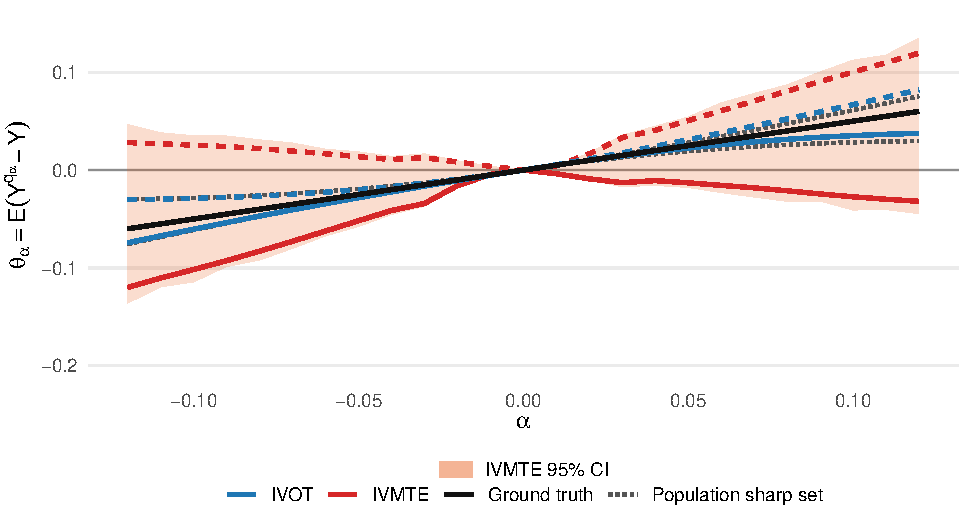
\includegraphics[width=\textwidth]{figures/prte_comparison_continuous_5000.pdf}
    \caption{Continuous-instrument IVOT and IVMTE identified sets for $\theta_\alpha = \mathbb{E}[Y^{q_\alpha}-Y]$ across policy shifts $\alpha \in [-0.12, 0.12]$ at $n=5{,}000$. Grey dotted curves: the population sharp identified set, computed in closed form. Black line: ground truth. Blue and red curves: estimated IVOT and IVMTE bounds (solid = lower, dashed = upper). Shaded ribbon: pointwise 95\% backward confidence interval for the IVMTE bounds.}
    \label{fig:synthetic_bounds}
\end{figure}

\paragraph{Discrete instrument.}
The discrete-instrument DGP uses $Z \sim \text{Bernoulli}(0.5)$ with two-point propensity score $\{0.25, 0.75\}$, to which the closed-form bounds of \cref{thm:discrete_lower_bound} apply, and a heterogeneous $\text{MTE}(u) = 0.48 + 0.18u$. The outcome support is $[0, 1.08]$ and the exact policy-effect truth is $\theta_\alpha = 0.57\alpha + 0.09\alpha^2$; both are derived in \cref{app:simulation}. \cref{fig:synthetic_bounds_discrete} shows the identified sets at $n = 5{,}000$ alongside the population sharp set. The truth falls inside the IVOT interval at all 25 grid points, and the IVOT interval is $2.4$--$3.6\times$ narrower than IVMTE throughout: at $\alpha = 0.05$ the IVOT interval is $[-0.001,\, 0.042]$ (width $0.043$) versus the IVMTE interval $[-0.051,\, 0.054]$ (width $0.105$). The gap between the two methods is enough to change the qualitative conclusion at large shifts: the estimated IVMTE identified set contains zero at every $\alpha$, whereas the estimated IVOT identified set excludes zero once $\alpha \geqslant 0.08$.

\begin{figure}[!htbp]
    \centering
    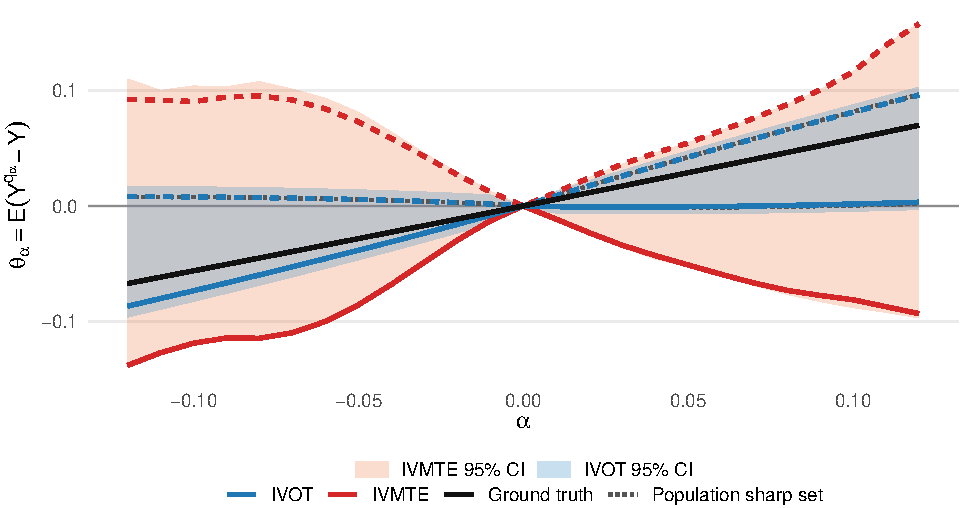
\includegraphics[width=\textwidth]{figures/prte_comparison_discrete.pdf}
    \caption{Discrete-instrument IVOT and IVMTE identified sets for $\theta_\alpha = \mathbb{E}[Y^{q_\alpha}-Y]$ across policy shifts $\alpha \in [-0.12, 0.12]$ at $n=5{,}000$. Grey dotted curves: the population sharp identified set, computed in closed form. Black line: ground truth. Blue and red curves: estimated IVOT and IVMTE bounds (solid = lower, dashed = upper). Shaded ribbons: pointwise 95\% confidence intervals for the bounds (blue = IVOT delta method, red = IVMTE backward CI).}
    \label{fig:synthetic_bounds_discrete}
\end{figure}

\paragraph{Discrete instrument with covariates.}
The third design adds five continuous covariates to a three-valued instrument, with $\text{MTE}(u,x)$ varying in both arguments, and is built so that \cref{asp:prop_gap} holds exactly with $c_{\text{gap}}=0.04$ and every component of the score is active on the reported window $\alpha\in[0.195,0.255]$, at $n=4{,}000$. As in the two designs above the comparison is against IVMTE in its nonparametric form, so the $u$-spline sieve is interacted with the covariates and the MTR is left unrestricted in shape as well as in level. \Cref{app:simulation} of \oalocation{} gives the DGP, the policy window, the comparison choices, and the numerical tables.

\cref{fig:synthetic_bounds_cov} shows the estimated IVOT interval tracking the population sharp set---closed form here up to the expectation over $X$---and containing the truth at all $11$ grid points, at $0.79$--$1.06$ times the sharp width. IVOT is narrower than IVMTE by $1.10$--$1.46\times$ at degree $3$ and $1.34$--$1.78\times$ at degree $7$, and the difference is qualitative: at $\alpha = 0.219$ the sharp set is $[0.019,\,0.134]$ and IVOT $[0.015,\,0.137]$, while IVMTE at degree $7$ returns $[-0.012,\,0.156]$. Both that interval and its pointwise 95\% backward confidence band contain zero throughout the policy-shift grid, so the moment relaxation loses the sign of the policy effect.

\begin{figure}[!htbp]
    \centering
    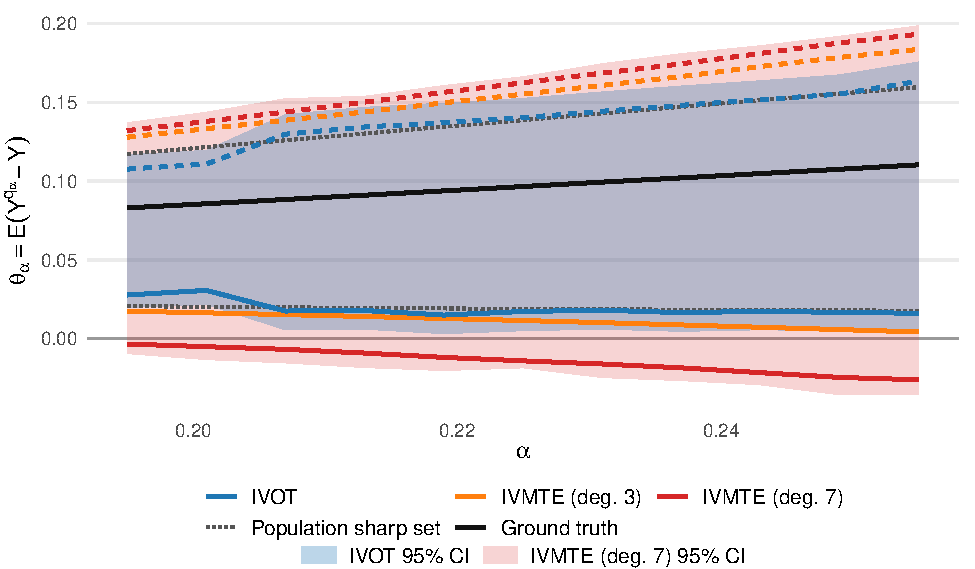
\includegraphics[width=\textwidth]{figures/prte_comparison_discrete_cov.pdf}
    \caption{Covariate design: IVOT and IVMTE identified sets for $\theta_\alpha = \mathbb{E}[Y^{q_\alpha}-Y]$ at $n=4{,}000$, with five continuous covariates and a three-valued instrument. Grey dotted curves: the population sharp identified set, computed in closed form. Black line: ground truth. Blue: IVOT (solid = lower, dashed = upper), with its pointwise 95\% interval shaded. Orange and red: IVMTE with the $u$-spline sieve interacted with the covariates, at degrees $3$ and $7$. The red shading is the pointwise 95\% backward bootstrap confidence band for the degree-$7$ IVMTE bounds. As in \cref{fig:bednet_bounds}, the richer sieve gives the wider bound.}
    \label{fig:synthetic_bounds_cov}
\end{figure}

The estimation theory of \cref{sec:est_inf} is tested separately by Monte Carlo. Over $400$ replications at each of five sample sizes from $1{,}000$ to $16{,}000$ the sampling standard deviation contracts at the parametric rate, the estimated standard errors closely match the Monte Carlo standard deviations at the larger sample sizes---their ratios rise to $1.00$ and $1.02$ for the two bounds---and the level-set recovery step returns the correct configuration in every replication once $n\geqslant8{,}000$. \Cref{app:simulation} of \oalocation{} gives the full Monte Carlo results.

\FloatBarrier
\subsection{Effect of Price Subsidies for Bed Nets}\label{sec:sim_bednet}

\paragraph{Background and setup.}
We apply our method to the bed net subsidy experiment of \citet{dupas2014subsidies}. The policy question is how the price of a bed net affects its usage, which is what a PRTE measures. For $n = 1{,}078$ Kenyan households the data contain the offered price as instrument $Z$ (17 values spanning 0--250 KSh, randomized across distribution points), purchase as treatment $W$, and one-year follow-up usage as outcome $Y$. We compare two fixed-price policies: the baseline assigns every household the reference price $z_0 = 150$ KSh, and for each $\alpha \in [0.05, 0.62]$ the alternative raises the purchase propensity from $\hat p(z_0)$ to $q_\alpha := \min(\hat{p}(z_0) + \alpha, 1)$. The target is $\text{PRTE}_\alpha = \mathbb{E}[Y^{q_\alpha} - Y^{p(z_0)}]/\alpha$; because both policies are constant in $Z$, the mean policy shift equals $\alpha$ exactly, so the denominator is the shift size rather than an estimated quantity. The baseline is the fixed-price policy $Y^{p(z_0)}$, not the observed $Y$ under randomized prices, and the grid is itself constructed from the first stage, its endpoint $\alpha_{\max}\approx 0.621$ being the estimated propensity at zero price minus the estimated baseline propensity. Because the instrument is discrete, the closed-form bounds of \cref{thm:discrete_lower_bound} apply directly to the numerator, after which we divide by $\alpha$. For IVMTE, we approximate the marginal treatment response (MTR) functions with degree-$10$ and degree-$20$ $u$-spline sieves on $[0,1]$. Full data, propensity-estimation, and policy-construction details are in \cref{app:simulation}.

\begin{figure}[!htbp]
    \centering
    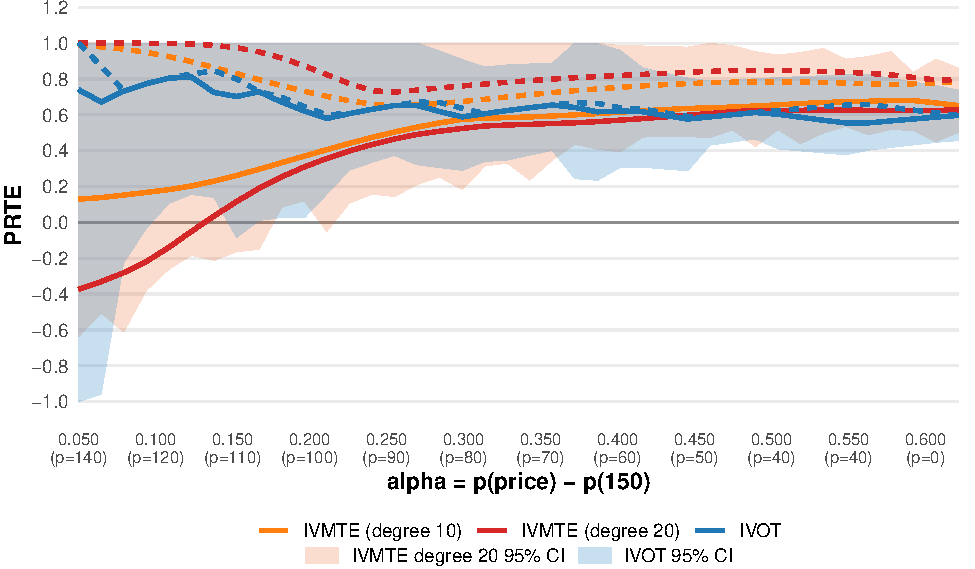
\includegraphics[width=\textwidth]{figures/prte_comparison_bednet.pdf}
    \caption{IVOT versus IVMTE identified sets for $\text{PRTE}_\alpha = \mathbb{E}[Y^{q_\alpha}-Y^{p(z_0)}]/\alpha$ on the bed net data from \citet{dupas2014subsidies}. IVMTE is shown for degree-$10$ (orange) and degree-$20$ (red) $u$-spline sieves, with solid curves the lower bounds and dashed the upper; degree~$20$ widens the bound, reflecting the more nonparametric MTR class. Shaded ribbons: pointwise 95\% confidence intervals for the estimated bounds (red = IVMTE deg.~$20$, blue = IVOT). IVOT substantially tightens the identified set and achieves near-point identification at several subsidy levels.}
    \label{fig:bednet_bounds}
\end{figure}

\paragraph{Results.}
\cref{fig:bednet_bounds} plots the IVOT and IVMTE identified sets for $\text{PRTE}_\alpha$ across subsidy levels. IVOT consistently yields a tighter identified set than IVMTE across the reported range of $\alpha$ and at both spline degrees. At the smallest subsidy ($\alpha = 0.05$), the IVOT interval is $3.3$ times narrower than IVMTE at degree $10$ and $5.3$ times narrower at degree $20$.

Both methods indicate a positive policy effect across most of the subsidy range---the IVOT lower bound is positive throughout, and the degree-$10$ IVMTE lower bound is positive for all $\alpha$, with the more conservative degree-$20$ lower bound turning positive once $\alpha \geqslant 0.14$. IVOT achieves near-point identification (width $< 0.05$) for the majority of $\alpha$ values. Those narrow identified sets do not translate one-for-one into narrower confidence intervals. \cref{app:simulation} gives more details and explanations for the wide confidence intervals.



\section{Conclusion}\label{sec:conclusion}
We connected the partial identification of PRTEs in IV models to OT: formulating it as a CCOT problem over the joint laws compatible with the observed data, we showed that the multidimensional optimization reduces analytically to one-dimensional OT problems with product costs, yielding closed-form sharp bounds and bypassing the numerical optimization that existing computational approaches require. In a companion note we replace threshold crossing by a conditional quantile representation of the selection equation and obtain sharp closed-form bounds for continuous and multi-valued treatments, under a rank-overlap condition in the strictly monotonic case and an algebraic condition on the instrument-induced latent intervals in the ordered-choice case. The estimation theory developed here is for binary treatments, delivering $\sqrt{n}$-consistency and asymptotic normality with discrete instruments under the stated regularity conditions, and nonparametric convergence rates with continuous ones.

The central insight, demonstrated theoretically and empirically, is that preserving full distributional information is tractable and valuable for tight partial identification: moment-relaxation approaches reduce the observed data to conditional expectations and can produce substantially wider bounds, whereas CCOT enforces compatibility with the entire observed distribution while keeping the optimization transparent. We expect this to extend beyond the IV setting studied here.


\paragraph{Acknowledgments.} Jose Blanchet gratefully acknowledges support from the U.S. Department of Defense through the Air Force Office of Scientific Research award FA9550-20-1-0397 and ONR award 1398311, as well as support from NSF grants 2229012, 2312204, and 2403007.
Vasilis Syrgkanis gratefully acknowledges support from NSF Award IIS-2337916, an Amazon Research Award, and a Google Research Award.




\bibliographystyle{plainnat}
\bibliography{ref}


\newpage
\appendix
% Main identification and inference proofs, algorithms, and score constructions.
\section{Proofs in \protect\NoCaseChange{\cref{sec:pid}}}\label{app:proofs_pid}

\subsection{Proof of Sharpness}

\begin{proof}[Proof of \cref{prop:sharpness}]
    \noindent\textbf{Direct direction.}
    Let $\tilde{\pi}$ be a probability measure on $\mathcal{Y}^2 \times [0,1] \times \mathcal{X}$ whose $(Y(w), U, X)$-marginals satisfy $(\tilde{\pi}_0,\tilde{\pi}_1) \in \Gamma(\mathbb{P}_{\text{obs}})$. By the constraints in~(\ref{eq:ot_formulation}), each $\tilde{\pi}_w$ is a probability measure on $\mathcal{Y} \times [0,1] \times \mathcal{X}$ satisfying:
    \begin{enumerate}
        \item[(C1)] $\displaystyle \int_0^{p(z,x)} \tilde{\pi}_1(\mathrm{d}y \mid u, x) \, \mathrm{d}u = H_{1,x}(p(z,x),\mathrm{d}y)$, for $\mathbb{P}_{\text{obs}}$-a.e.\ $(z,x)$;
        \item[(C2)] $\displaystyle \int_{p(z,x)}^{1} \tilde{\pi}_0(\mathrm{d}y \mid u, x) \, \mathrm{d}u = H_{0,x}(p(z,x),\mathrm{d}y)$, for $\mathbb{P}_{\text{obs}}$-a.e.\ $(z,x)$;
        \item[(C3)] $\tilde{\pi}_w(\mathrm{d}u, \mathrm{d}x) = \mathrm{d}u \, \mathbb{P}_{\text{obs}}(\mathrm{d}x)$ for $w \in \{0,1\}$.
    \end{enumerate}
    Since $\mathcal{Y}^2 \subseteq \mathbb{R}^2$ is a Polish space and the $(U, X)$-marginal of $\tilde{\pi}$ is $\mathrm{d}u \, \mathbb{P}_{\text{obs}}(\mathrm{d}x)$ by (C3) applied to either marginal, $\tilde{\pi}$ admits a regular conditional kernel $\tilde{\pi}(\mathrm{d}y_0, \mathrm{d}y_1 \mid u, x)$ for $(\mathrm{d}u \otimes \mathbb{P}_{\text{obs}}(\mathrm{d}x))$-a.e.\ $(u, x)$, whose $Y(0)$- and $Y(1)$-marginals recover $\tilde{\pi}_0(\mathrm{d}y_0 \mid u, x)$ and $\tilde{\pi}_1(\mathrm{d}y_1 \mid u, x)$ respectively.

    \medskip
    \noindent\textbf{Construction.}
    We construct the joint distribution $\mathbb{P}$ of $(Y(0), Y(1), U, X, Z, W)$ on the product space $\mathcal{Y}^2 \times [0,1] \times \mathcal{X} \times \mathcal{Z} \times \{0,1\}$ via the following disintegration:
    \begin{equation}\label{eq:sharp_construct}
        \mathbb{P}(\mathrm{d}y_0, \mathrm{d}y_1, \mathrm{d}u, \mathrm{d}x, \mathrm{d}z, \{w\})
        = \tilde{\pi}(\mathrm{d}y_0, \mathrm{d}y_1 \mid u, x) \, \mathrm{d}u \, \mathbb{P}_{\text{obs}}(\mathrm{d}z \mid x) \, \mathbb{P}_{\text{obs}}(\mathrm{d}x) \, \delta_{\indicator(u \leqslant p(z,x))}(\{w\}),
    \end{equation}
    where $\delta_{\indicator(u \leqslant p(z,x))}(\{w\})$ is the Dirac mass placing all weight on $w = \indicator(u \leqslant p(z,x))$, enforcing the threshold-crossing selection rule deterministically. Crucially, $(Y(0), Y(1))$ are drawn jointly from $\tilde{\pi}(\cdot \mid u, x)$, so the coupling prescribed by $\tilde{\pi}$ is preserved conditional on $(U, X)$; the independent coupling $\tilde{\pi}_0(\mathrm{d}y_0 \mid u, x) \, \tilde{\pi}_1(\mathrm{d}y_1 \mid u, x)$ is one feasible choice among many. The measure in~(\ref{eq:sharp_construct}) is well-defined because the kernels are measurable and all component measures are probability measures.

    \medskip
    \noindent\textbf{Proof of (i): joint marginal distribution.}
    We show that the $(Y(0), Y(1), U, X)$-marginal of $\mathbb{P}$ equals $\tilde{\pi}$. Marginalizing~(\ref{eq:sharp_construct}) over $(Z, W)$:
    \begin{align*}
        \mathbb{P}(\mathrm{d}y_0, \mathrm{d}y_1, \mathrm{d}u, \mathrm{d}x)
        &= \tilde{\pi}(\mathrm{d}y_0, \mathrm{d}y_1 \mid u, x) \, \mathrm{d}u \, \mathbb{P}_{\text{obs}}(\mathrm{d}x) \underbrace{\sum_{w \in \{0, 1\}} \int_{\mathcal{Z}} \delta_{\indicator(u \leqslant p(z,x))}(\{w\}) \, \mathbb{P}_{\text{obs}}(\mathrm{d}z \mid x)}_{=\, 1} \\
        &= \tilde{\pi}(\mathrm{d}y_0, \mathrm{d}y_1 \mid u, x) \, \mathrm{d}u \, \mathbb{P}_{\text{obs}}(\mathrm{d}x).
    \end{align*}
    By (C3) the $(U, X)$-marginal of $\tilde{\pi}$ is $\mathrm{d}u \, \mathbb{P}_{\text{obs}}(\mathrm{d}x)$, so the right-hand side equals
    \begin{equation*}
        \tilde{\pi}(\mathrm{d}y_0, \mathrm{d}y_1, \mathrm{d}u, \mathrm{d}x),
    \end{equation*}
    establishing (i).

    \medskip
    \noindent\textbf{Proof of (ii): structural assumptions.}
    We establish each part of \cref{asp:structure}.
    \begin{itemize}
        \item \textbf{Consistency.} Consistency holds trivially by setting the observed outcome to be $Y = W Y(1) + (1-W) Y(0)$.
        \item \textbf{Conditional instrumental exogeneity.} By~(\ref{eq:sharp_construct}), conditional on $X = x$, the variables $(Y(0), Y(1), U)$ are drawn from $\tilde{\pi}(\mathrm{d}y_0, \mathrm{d}y_1 \mid u, x) \, \mathrm{d}u$ and $Z$ is drawn independently from $\mathbb{P}_{\text{obs}}(\mathrm{d}z \mid x)$. These appear as independent factors in~(\ref{eq:sharp_construct}), so $Z \indep (Y(0), Y(1), U) \mid X$ under $\mathbb{P}$.
        \item \textbf{Threshold crossing.} The selection equation $W = \indicator(U \leqslant p(Z,X))$ holds $\mathbb{P}$-a.s.\ by the Dirac mass in~(\ref{eq:sharp_construct}). Moreover, (C3) gives $U \mid X \sim \mathrm{Unif}(0,1)$. Conditional instrumental exogeneity then yields $\mathbb P(W=1\mid Z=z,X=x)=p(z,x)$ for $\mathbb P_{Z,X}$-almost every $(z,x)$.
        \item \textbf{Common instrument support.} The construction preserves the observed conditional law $\mathbb P_{\mathrm{obs}}(\mathrm dz\mid x)$. Because the proposition assumes that $\mathbb P_{\mathrm{obs}}$ is generated by a model satisfying \cref{asp:structure}, its common-support property is inherited by the constructed model.
    \end{itemize}

    \medskip
    \noindent\textbf{Proof of (iii): observational equivalence.}
    We must show that the distribution of the observables $(Y, Z, X, W)$ induced by $\mathbb{P}$ coincides with $\mathbb{P}_{\text{obs}}$. Since the marginal of $(Z, X)$ under $\mathbb{P}$ equals $\mathbb{P}_{\text{obs}}(Z, X)$ by construction, it suffices to show that the conditional laws of $(Y, W)$ given $(Z, X)$ agree.

    Fix $(z, x)$ and consider the event $W = 1$. Under $\mathbb{P}$, marginalizing~(\ref{eq:sharp_construct}) over $(Y(0), Y(1))$ reduces the joint kernel to its $Y(1)$-marginal $\tilde{\pi}_1(\cdot \mid u, x)$; using $W = 1 \Leftrightarrow U \leqslant p(z,x)$ and $Y = Y(1)$ when $W = 1$,
    \begin{align*}
        \mathbb{P}(Y \in A, \, W = 1 \mid Z = z, X = x)
        &= \int_0^{p(z,x)} \tilde{\pi}_1(A \mid u, x) \, \mathrm{d}u.
    \end{align*}
    By constraint (C1), this equals $H_{1,x}(p(z,x),A)$, which is the observed conditional subdistribution $\mathbb{P}_{\text{obs}}(Y \in A, \, W = 1 \mid Z = z, X = x)$ for $\mathbb P_{Z,X}$-almost every $(z,x)$. Similarly, for $W = 0$ we have $Y = Y(0)$ and $U > p(z, x)$, so marginalizing over $(Y(0), Y(1))$ leaves the $Y(0)$-marginal $\tilde{\pi}_0$ and
    \begin{align*}
        \mathbb{P}(Y \in A, \, W = 0 \mid Z = z, X = x)
        &= \int_{p(z,x)}^{1} \tilde{\pi}_0(A \mid u, x) \, \mathrm{d}u,
    \end{align*}
    which equals $H_{0,x}(p(z,x),A)$ by constraint (C2), and hence equals the corresponding observed conditional subdistribution almost surely. Thus the conditional laws of $(Y, W) \mid (Z, X)$ under $\mathbb{P}$ and $\mathbb{P}_{\text{obs}}$ agree for both values of $W$, which proves (iii).

    \medskip
    \noindent\textbf{Converse direction.}
    Suppose $(Y(0), Y(1), U, X, Z, W)$ is a joint distribution satisfying (ii)--(iii), and let $\tilde{\pi}$ denote its $(Y(0), Y(1), U, X)$-marginal. Fix $w \in \{0, 1\}$. The $(U, X)$-marginal of $\tilde{\pi}_w$ equals the $(U, X)$-marginal of $\tilde{\pi}$; by \cref{asp:structure} (threshold crossing), $U \mid X \sim \mathrm{Unif}(0, 1)$ and $X$ has marginal $\mathbb{P}_{\text{obs}}(\mathrm{d}x)$ under (iii), so $\tilde{\pi}_w(\mathrm{d}u, \mathrm{d}x) = \mathrm{d}u \, \mathbb{P}_{\text{obs}}(\mathrm{d}x)$, establishing (C3). For (C1), using consistency and the selection rule $W = \indicator(U \leqslant p(Z, X))$ together with conditional instrumental exogeneity,
    \begin{align*}
        \mathbb{P}_{\text{obs}}(Y \in A, \, W = 1 \mid Z = z, X = x)
        &= \mathbb{P}(Y(1) \in A, \, U \leqslant p(z, x) \mid Z = z, X = x) \\
        &= \int_0^{p(z, x)} \tilde{\pi}_1(A \mid u, x) \, \mathrm{d}u,
    \end{align*}
    where the second equality uses $Z \indep (Y(1), U) \mid X$ and $U \mid X \sim \mathrm{Unif}(0, 1)$. Property (iii) identifies the left-hand side with the observational conditional distribution. By the propensity-score sufficiency argument preceding~(\ref{eq:canonical_submeasures}), its canonical propensity-indexed version is $H_{1,x}(p(z,x),A)$, yielding (C1). The argument for (C2) is symmetric. Therefore $(\tilde{\pi}_0,\tilde{\pi}_1) \in \Gamma(\mathbb{P}_{\text{obs}})$, completing the converse.
\end{proof}

% The following discrete-case covariate proof is retained (commented out) for
% future reference. The unified proof of \cref{thm:covariate_continuous_lower_bound}
% below now covers this case as a special instance (every LIV interval degenerate).
\iffalse
\subsection{Proof of \cref{thm:covariate_discrete_lower_bound}}

\begin{proof}[Proof of \cref{thm:covariate_discrete_lower_bound}]
We prove the sharp lower bound; the upper bound follows by an identical argument with the comonotonic coupling replacing the countermonotonic one and swapping $y_{\min}$ and $y_{\max}$ in the trivial bound term.

\medskip
\noindent\textbf{Disintegration over $X$.}
Recall that the $W=1$ side minimization problem~(\ref{eq:ot_formulation_1}) reads
\begin{equation*}
    \min_{\pi_1 \in \Gamma_1(\mathbb{P}_{\text{obs}})} \mathbb{E}_{\pi_1}[Y(1)\,\omega(X,U)],
\end{equation*}
where $\Gamma_1(\mathbb{P}_{\text{obs}})$ denotes the set of probability measures $\pi_1$ on $\mathcal{Y} \times [0,1] \times \mathcal{X}$ satisfying
\begin{align}
    &\int_0^{p(z,x)} \pi_1(\mathrm{d}y \mid u, x)\,\mathrm{d}u = \mathbb{P}_{\text{obs}}(\mathrm{d}y, W\!=\!1 \mid p(Z,X)\!=\!p(z,x), X\!=\!x), \quad \text{for } \mathbb{P}_{\text{obs}}\text{-a.e.\ } (z,x), \label{eq:pf_constraint1} \\
    &\pi_1(\mathrm{d}u, \mathrm{d}x) = \mathrm{d}u\;\mathbb{P}_{\text{obs}}(\mathrm{d}x). \label{eq:pf_constraint2}
\end{align}
The conditional distribution in RHS of (\ref{eq:pf_constraint1}) is well-defined because of \cref{asp:structure}.(4). By the marginal constraint~(\ref{eq:pf_constraint2}), we can disintegrate $\pi_1$ with respect to the $(U,X)$-marginal and write the objective as an iterated integral:
\begin{equation}\label{eq:pf_iterated}
    \mathbb{E}_{\pi_1}[Y(1)\,\omega(X,U)] = \mathbb{E}_{X}\left[\int_0^1 \left(\int_{\mathcal{Y}} y\;\pi_1(\mathrm{d}y \mid u, X)\right) \omega(X,u)\,\mathrm{d}u\right].
\end{equation}
The observational constraint~(\ref{eq:pf_constraint1}) couples the conditional kernel $\pi_1(\mathrm{d}y \mid u, x)$ across different values of $u$ only through the integral $\int_0^{p(z,x)} \pi_1(\mathrm{d}y \mid u, x)\,\mathrm{d}u$, which for a fixed $x$ involves only the kernel values at that same $x$. Therefore, the constraints decouple across $x$: the kernel $\pi_1(\cdot \mid \cdot, x)$ is constrained independently for $\mathbb{P}_{\text{obs}}$-a.e.\ $x$. Writing $B_Y=\max\{|y_{\min}|,|y_{\max}|\}$, every feasible conditional objective is dominated in absolute value by $B_Y\int_0^1|\omega(x,u)|\,\mathrm du$, whose expectation is finite by \cref{asp:target_weight}. We may therefore exchange the minimization and the outer expectation over $X$ by a standard measurable selection argument \citep[Proposition 7.50]{bertsekas1996stochastic}:
\begin{equation}\label{eq:pf_exchange}
    \min_{\pi_1 \in \Gamma_1(\mathbb{P}_{\text{obs}})} \mathbb{E}_{\pi_1}[Y(1)\,\omega(X,U)] = \mathbb{E}_{X}\left[\min_{\pi_{1,X} \in \Gamma_{1,X}} \int_0^1 \left(\int_{\mathcal{Y}} y\;\pi_{1,X}(\mathrm{d}y \mid u)\right) \omega(X,u)\,\mathrm{d}u\right],
\end{equation}
where $\Gamma_{1,X}$ denotes the set of probability kernels $\pi_{1,X}(\mathrm{d}y \mid u)$ on $\mathcal{Y} \times [0,1]$ satisfying the constraint~(\ref{eq:pf_constraint1}) with $x = X$ held fixed.

\medskip
\noindent\textbf{Decomposition into sub-interval problems.}
Fix $x \in \mathcal{X}$. Since $\mathcal{Z}$ is finite, the conditional propensity score $p(z,x)$ takes finitely many distinct values, which we order as $0 = p_0(x) \leqslant p_1(x) < \cdots < p_{K_x}(x) \leqslant p_{K_x+1}(x) = 1$. This partitions $[0,1]$ into $K_x + 1$ disjoint sub-intervals $I_i(x) = (p_i(x), p_{i+1}(x)]$ for $i = 0, \ldots, K_x$.

The inner integral in~(\ref{eq:pf_exchange}) decomposes additively:
\begin{equation}\label{eq:pf_decompose}
    \int_0^1 \left(\int_{\mathcal{Y}} y\;\pi_{1,x}(\mathrm{d}y \mid u)\right)\omega(x,u)\,\mathrm{d}u = \sum_{i=0}^{K_x} \int_{I_i(x)} \left(\int_{\mathcal{Y}} y\;\pi_{1,x}(\mathrm{d}y \mid u)\right)\omega(x,u)\,\mathrm{d}u.
\end{equation}

We now show that the constraints also decouple across these sub-intervals. The observational constraint~(\ref{eq:pf_constraint1}) at the $x$-slice reads: for every $j = 1, \ldots, K_x$,
\begin{equation}\label{eq:pf_obs_j}
    \int_0^{p_j(x)} \pi_{1,x}(\mathrm{d}y \mid u)\,\mathrm{d}u = \mathbb{P}_{\text{obs}}(\mathrm{d}y, W\!=\!1 \mid p(Z,x) = p_j(x), X = x).
\end{equation}
Telescoping: for $i = 0, \ldots, K_x - 1$, subtracting the constraint at $p_i(x)$ from that at $p_{i+1}(x)$ (with the convention that the left-hand side at $p_0(x) = 0$ is zero) yields
\begin{equation}\label{eq:pf_telescope}
   \begin{split}
        \int_{I_i(x)} \pi_{1,x}(\mathrm{d}y \mid u)\,\mathrm{d}u &= \mathbb{P}_{\text{obs}}(\mathrm{d}y, W\!=\!1 \mid p(Z,x)\!=\!p_{i+1}(x), X\!=\!x) \\
        &\quad\quad - \mathbb{P}_{\text{obs}}(\mathrm{d}y, W\!=\!1 \mid p(Z,x)\!=\!p_i(x), X\!=\!x).
   \end{split}
\end{equation}
Dividing both sides by $|I_i(x)| = p_{i+1}(x) - p_i(x) > 0$, we see that the constraint fixes the marginal distribution of $Y(1)$ conditional on $U \in I_i(x)$ and $X = x$ to be exactly the identified measure $\mu_{1, i \mid x}$ defined in the theorem statement. Since cumulative sums over the telescoped constraints recover the original system~(\ref{eq:pf_obs_j}), this transformation is invertible, and hence the two systems of constraints are equivalent.

Crucially, this constraint involves only the kernel $\pi_{1,x}(\mathrm{d}y \mid u)$ for $u \in I_i(x)$ and is independent of the kernel on any other sub-interval. Since the objective~(\ref{eq:pf_decompose}) is also additively separable, the conditional minimization problem at $X = x$ decomposes into $K_x + 1$ independent sub-problems.

\medskip
\noindent\textbf{Solving the sub-interval OT problems.}
For each $i = 0, \ldots, K_x - 1$, the $i$-th constrained sub-problem is:
\begin{equation}\label{eq:pf_sub_i}
    (p_{i+1}(x)-p_i(x))\min_{\gamma_i \in \Pi(\mu_{1, i \mid x},\, \nu_{i \mid x})} \int_{\mathcal{Y} \times I_i(x)} y \cdot \omega(x,u)\,\mathrm{d}\gamma_i(y,u),
\end{equation}
where $\nu_{i \mid x} = \mathrm{Unif}(p_i(x), p_{i+1}(x))$ is the (known) marginal of $U$ on $I_i(x)$. The set of feasible joint distributions of $(Y(1), U)$ on $\mathcal{Y} \times I_i(x)$ with the prescribed marginals is exactly the set of couplings $\Pi(\mu_{1, i \mid x}, \nu_{i \mid x})$.

Let $\rho_{i\mid x}$ be the pushforward of $\nu_{i\mid x}$ under $u\mapsto\omega(x,u)$. Pushing a coupling of $(Y,U)$ forward to $(Y,\omega(x,U))$, and conversely lifting any coupling of $(Y,\omega(x,U))$ through a regular conditional law of $U$ given $\omega(x,U)$, shows that the subproblem is equivalent to product-cost transport between $\mu_{1,i\mid x}$ and $\rho_{i\mid x}$. Let $Q_{Y, i \mid x}$ denote the quantile function of $\mu_{1, i \mid x}$ and $Q_{\omega, i \mid x}$ denote the quantile function of $\rho_{i\mid x}$. Then \cref{thm:1d_ot} gives
\begin{equation}\label{eq:pf_ot_sol}
    \min_{\gamma_i \in \Pi(\mu_{1, i \mid x},\, \nu_{i \mid x})} \int y \cdot \omega(x,u)\,\mathrm{d}\gamma_i = \int_0^1 Q_{Y, i \mid x}(t)\,Q_{\omega, i \mid x}(1-t)\,\mathrm{d}t.
\end{equation}
The interval-length prefactor already appears outside the probability-coupling problem in~(\ref{eq:pf_sub_i}); no second factor enters the coupling optimum.

\medskip
\noindent\textbf{The unconstrained interval.}
For the final interval $I_{K_x}(x) = (p_{K_x}(x), 1]$, no instrument value produces a propensity score exceeding $p_{K_x}(x)$, so the potential outcome $Y(1)$ is never observed for this subpopulation. The constraint~(\ref{eq:pf_obs_j}) does not restrict $\pi_{1,x}(\mathrm{d}y \mid u)$ for $u \in I_{K_x}(x)$, and the minimization is unconstrained. Because $y_{\min}$ and $y_{\max}$ are the extrema of the compact outcome domain, for each $u \in I_{K_x}(x)$ the pointwise minimum of the integrand $\int_{\mathcal{Y}} y\;\pi_{1,x}(\mathrm{d}y \mid u)\cdot\omega(x,u)$ is achieved by $\pi_{1,x}(\cdot \mid u) = \delta_{y_{\min}}$ when $\omega(x,u) \geqslant 0$ and by $\pi_{1,x}(\cdot \mid u) = \delta_{y_{\max}}$ when $\omega(x,u) < 0$:
\begin{equation}\label{eq:pf_trivial}
    \min \int_{I_{K_x}(x)} \left(\int_{\mathcal{Y}} y\;\pi_{1,x}(\mathrm{d}y \mid u)\right)\omega(x,u)\,\mathrm{d}u = \int_{p_{K_x}(x)}^1 \Big(y_{\min}\max\{0,\omega(x,u)\} + y_{\max}\min\{0,\omega(x,u)\}\Big)\mathrm{d}u.
\end{equation}

\medskip
\noindent\textbf{Aggregation over $X$.}
Combining (\ref{eq:pf_ot_sol}) and (\ref{eq:pf_trivial}) into~(\ref{eq:pf_exchange}), we obtain
\begin{align*}
    \underline{\theta}_{\omega,1} &= \mathbb{E}_{X}\Big[\sum_{i=0}^{K_X-1} (p_{i+1}(X) - p_i(X)) \int_0^1 Q_{Y, i \mid X}(t)\,Q_{\omega, i \mid X}(1-t)\,\mathrm{d}t \\
    &\quad\quad\quad\quad+ \int_{p_{K_X}(X)}^1 \Big(y_{\min}\max\{0,\omega(X,u)\} + y_{\max}\min\{0,\omega(X,u)\}\Big)\mathrm{d}u\Big].
\end{align*}
The outer expectation over $X$ is well-defined. Writing $B_Y=\max\{|y_{\min}|,|y_{\max}|\}$, the absolute value of the bracketed contribution is bounded by $B_Y\int_0^1|\omega(x,u)|\,\mathrm du$, whose expectation is finite by \cref{asp:target_weight}.

\medskip
\noindent\textbf{Sharpness.}
The bound is sharp because: (i) By \cref{prop:sharpness}, every feasible pair $(\pi_0, \pi_1) \in \Gamma(\mathbb{P}_{\text{obs}})$ corresponds to a valid data-generating process satisfying \cref{asp:structure}, so the infimum of $\theta_\omega$ over $\Gamma(\mathbb{P}_{\text{obs}})$ equals the infimum over all observationally equivalent structural models; and (ii) the infimum in each conditional sub-problem~(\ref{eq:pf_sub_i}) is attained by the countermonotonic coupling (which exists since $\mu_{1,i\mid x}$ and $\nu_{i\mid x}$ are Borel probability measures on $\mathbb{R}$), and the infimum in the unconstrained problem~(\ref{eq:pf_trivial}) is attained by the Dirac mass at $y_{\min}$ where $\omega(x,u) \geqslant 0$ and at $y_{\max}$ where $\omega(x,u) < 0$. By a measurable selection argument, these conditional optimizers can be assembled into a globally feasible $\pi_1^\star \in \Gamma_1(\mathbb{P}_{\text{obs}})$ that attains the global infimum.
\end{proof}
\fi

\subsection{Proof of \cref{thm:covariate_continuous_lower_bound}} \label{sec:cov_proof}

\begin{figure}[!htbp]
\centering
\begin{tikzpicture}[scale=1.0, font=\small]
  %% --- Layout (general instrument setting: $K=2$, order OT / LIV / OT / trivial) ---
  \def\W{12.0}    % full width (U = 1)
  \def\SH{1.10}   % main strip height
  \def\pOneL{2.5} % \underline{p}_1
  \def\pOneH{6.5} % \overline{p}_1
  \def\pTwo{9.0}  % p_2 — degenerate L_2 = \{p_2\}, marks the start of the trivial tail
  \def\qL{1.2}    % where omega begins descending
  \def\omY{2.20}  % omega baseline
  \def\omMax{1.80}% omega plateau height

  %% --- Main identification strip ---
  % G_0 = (0, \underline{p}_1): OT gap
  \fill[blue!18]    (0,0)        rectangle (\pOneL,\SH);
  % L_1 = [\underline{p}_1, \overline{p}_1]: non-degenerate LIV interval
  \fill[teal!18]    (\pOneL,0)   rectangle (\pOneH,\SH);
  % G_1 = (\overline{p}_1, p_2): OT gap
  \fill[blue!18]    (\pOneH,0)   rectangle (\pTwo,\SH);
  % Trivial tail (p_2, 1]
  \fill[orange!15]  (\pTwo,0)    rectangle (\W,\SH);
  \draw[thick]      (0,0)        rectangle (\W,\SH);
  % Vertical boundaries between regions
  \draw[thick, teal!55]   (\pOneL,0) -- (\pOneL,\SH);
  \draw[thick, blue!55]   (\pOneH,0) -- (\pOneH,\SH);
  % L_2 = \{p_2\}: degenerate LIV rendered as a thick teal line at the boundary to the trivial tail
  \draw[very thick, teal!70!black] (\pTwo,0) -- (\pTwo,\SH);

  % Region labels inside strip
  \node[blue!80!black,   font=\scriptsize\bfseries]  at (\pOneL/2,            0.72) {OT Gap};
  \node[blue!80!black,   font=\tiny]                 at (\pOneL/2,            0.30) {$G_0$};
  \node[teal!70!black,   font=\scriptsize\bfseries]  at ({(\pOneL+\pOneH)/2}, 0.72) {LIV Interval};
  \node[teal!70!black,   font=\tiny]                 at ({(\pOneL+\pOneH)/2}, 0.30) {$L_1$};
  \node[blue!80!black,   font=\scriptsize\bfseries]  at ({(\pOneH+\pTwo)/2},  0.72) {OT Gap};
  \node[blue!80!black,   font=\tiny]                 at ({(\pOneH+\pTwo)/2},  0.30) {$G_1$};
  \node[orange!80!black, font=\scriptsize\bfseries, align=center]
      at ({(\pTwo+\W)/2}, \SH/2) {Trivial\\[-1pt]Tail};

  % Degenerate LIV singleton label (above strip)
  \node[teal!55!black, font=\tiny, align=center]
      at (\pTwo, \SH+0.32) {degenerate\\[-1pt]$L_2=\{p_2\}$};

  %% --- U axis ---
  \draw[->,thick] (-0.3,-0.50) -- (\W+0.6,-0.50) node[right]{$U$};
  \draw (0,      -0.38) -- (0,      -0.60); \node[below,font=\scriptsize] at (0,      -0.60) {$0$};
  \draw (\pOneL, -0.38) -- (\pOneL, -0.60); \node[below,font=\scriptsize] at (\pOneL, -0.60) {$\underline{p}_1$};
  \draw (\pOneH, -0.38) -- (\pOneH, -0.60); \node[below,font=\scriptsize] at (\pOneH, -0.60) {$\overline{p}_1$};
  \draw (\pTwo,  -0.38) -- (\pTwo,  -0.60); \node[below,font=\scriptsize] at (\pTwo,  -0.60) {$p_2$};
  \draw (\W,     -0.38) -- (\W,     -0.60); \node[below,font=\scriptsize] at (\W,     -0.60) {$1$};

  %% --- Dashed vertical guides through all panels ---
  \draw[gray!40,dashed,thin] (\pOneL,-0.60) -- (\pOneL,{\omY+\omMax+0.25});
  \draw[gray!40,dashed,thin] (\pOneH,-0.60) -- (\pOneH,{\omY+\omMax+0.25});
  \draw[gray!40,dashed,thin] (\pTwo, -0.60) -- (\pTwo, {\omY+\omMax+0.25});

  %% --- Omega smooth-curve panel ---
  \draw[->,thick] (-0.3,\omY) -- (-0.3,{\omY+\omMax+0.55})
      node[above,font=\scriptsize]{$\omega(u)$};
  \draw[gray!30,thin] (0,\omY) -- (\W,\omY);      % zero baseline
  \node[left,font=\scriptsize,gray] at (-0.3,\omY) {$0$};

  % Smooth non-increasing omega curve
  \draw[thick, violet!80!black]
      (0, {\omY+\omMax}) -- (\qL, {\omY+\omMax})
      .. controls (2.0, {\omY+1.65}) and (\pOneL, {\omY+1.40}) ..
         (3.8, {\omY+1.05})
      .. controls (5.0, {\omY+0.80}) and (\pOneH, {\omY+0.55}) ..
         (7.3, {\omY+0.42})
      .. controls (8.2, {\omY+0.30}) and (\pTwo,  {\omY+0.20}) ..
         (10.0, {\omY+0.12})
      .. controls (11.0, {\omY+0.08}) and (11.5, {\omY+0.06}) ..
         (\W, {\omY+0.05});

  % LIV annotation: point-identified via derivative
  \node[font=\tiny,teal!65!black] at ({(\pOneL+\pOneH)/2},{\omY+1.50})
      {$\mathbb{E}[Y(1)\mid U\!=\!u]$ point-identified};

  %% --- Connecting arrows (strip to bound labels) ---
  \draw[->,dashed,blue!40]    (\pOneL/2,              0) -- (\pOneL/2,              -1.00);
  \draw[->,dashed,teal!50]    ({(\pOneL+\pOneH)/2},   0) -- ({(\pOneL+\pOneH)/2},   -1.00);
  \draw[->,dashed,blue!40]    ({(\pOneH+\pTwo)/2},    0) -- ({(\pOneH+\pTwo)/2},    -1.00);
  \draw[->,dashed,orange!55]  ({(\pTwo+\W)/2},        0) -- ({(\pTwo+\W)/2},        -1.00);

  %% --- Brief per-region bound labels ---
  \node[blue!75!black, font=\tiny, align=center]
      at (\pOneL/2, -1.38) {quantile\\pairing};
  \node[teal!70!black, font=\tiny, align=center]
      at ({(\pOneL+\pOneH)/2}, -1.38) {direct\\identification};
  \node[blue!75!black, font=\tiny, align=center]
      at ({(\pOneH+\pTwo)/2}, -1.38) {quantile\\pairing};
  \node[orange!80!black, font=\tiny, align=center]
      at ({(\pTwo+\W)/2}, -1.38) {assign $y_{\min}$};

  % plus signs between labels
  \node[font=\scriptsize] at ({(\pOneL/2 + (\pOneL+\pOneH)/2)/2},         -1.38) {$+$};
  \node[font=\scriptsize] at ({((\pOneL+\pOneH)/2 + (\pOneH+\pTwo)/2)/2}, -1.38) {$+$};
  \node[font=\scriptsize] at ({((\pOneH+\pTwo)/2 + (\pTwo+\W)/2)/2},      -1.38) {$+$};

  %% --- Global sharp lower bound formula ---
  \node[align=center, font=\scriptsize] at ({\W/2}, -2.30) {
    $
    \underline{\theta}_{\omega,1}
    \;=\; \displaystyle\sum_{k=0}^{K-1}(\underline{p}_{k+1}\!-\!\overline{p}_k)\!\int_0^1\! Q_{Y,k}(t)\,Q_{\omega,k}(1\!-\!t)\,\mathrm{d}t
    \;+\; \displaystyle\sum_{k=1}^{K}\!\int_{\underline{p}_k}^{\overline{p}_k}\!
      \tfrac{\mathrm{d}}{\mathrm{d}u}g_1^{\mathrm c}(u)
      \;\omega(u)\,\mathrm{d}u
    \;+\; \displaystyle\int_{\overline{p}_K}^{1}\!\bigl(y_{\min}[\omega]_+\!+y_{\max}[\omega]_-\bigr)\mathrm{d}u$
  };

\end{tikzpicture}
\caption{Decomposition of the unit interval $[0,1]$ for the sharp lower bound in the general instrument setting (\cref{thm:continuous_lower_bound}), illustrated with $K=2$ in the order OT / LIV / OT / trivial: the non-degenerate LIV interval $L_1 = [\underline{p}_1, \overline{p}_1]$ (teal strip) lies between two OT gaps, and the degenerate LIV singleton $L_2 = \{p_2\}$ (teal line) sits at the boundary of the trivial tail. \textbf{\color{blue!65}OT gaps} $G_0 = (0, \underline{p}_1)$ and $G_1 = (\overline{p}_1, p_2)$: only the aggregate distributions $\mu_{1,0}, \mu_{1,1}$ are identified, so the tight bound requires countermonotone quantile coupling. \textbf{\color{teal!65}LIV interval} $L_1$: the propensity score sweeps a full subinterval, so the standard LIV derivative point-identifies $\mathbb{E}[Y(1)\mid U=u]$ exactly; the singleton $L_2$ contributes a Lebesgue-null integral and drops out. \textbf{\color{orange!65}Trivial tail} $(p_2, 1]$: $Y(1)$ is never observed; the lower bound assigns $y_{\min}$ where $\omega(u)\geqslant 0$ and $y_{\max}$ where $\omega(u)<0$. Collapsing every LIV interval to a singleton recovers the discrete case (\cref{fig:decomposition}); taking $K=1$ with $\underline{p}_1<\overline{p}_1$ and no trailing singleton recovers the connected-continuous case.}
\label{fig:continuous_decomposition}
\end{figure}


\begin{proof}[Proof of \cref{thm:covariate_continuous_lower_bound}]
We prove the sharp lower bound; the upper bound follows by replacing the countermonotonic coupling with the comonotonic one and swapping $y_{\min}$ and $y_{\max}$ in the trivial bound term.

\medskip
\noindent\textbf{Disintegration over $X$.}
Recall that the $W=1$ side minimization problem~(\ref{eq:ot_formulation_1}) reads $\min_{\pi_1 \in \Gamma_1(\mathbb{P}_{\text{obs}})} \mathbb{E}_{\pi_1}[Y(1)\,\omega(X,U)]$, where $\Gamma_1(\mathbb{P}_{\text{obs}})$ is the set of probability measures on $\mathcal{Y} \times [0,1] \times \mathcal{X}$ satisfying
\begin{align}
    &\int_0^{p(z,x)} \pi_1(\mathrm{d}y \mid u, x)\,\mathrm{d}u = H_{1,x}(p(z,x),\mathrm{d}y),\ \mathbb{P}_{\text{obs}}\text{-a.e.\ } (z,x), \label{eq:pf_cts_constraint1} \\
    &\pi_1(\mathrm{d}u, \mathrm{d}x) = \mathrm{d}u\;\mathbb{P}_{\text{obs}}(\mathrm{d}x). \label{eq:pf_cts_constraint2}
\end{align}
The observational constraint~(\ref{eq:pf_cts_constraint1}) couples $\pi_1(\mathrm{d}y \mid u, x)$ across different $u$ only through the integral $\int_0^{p(z,x)} \pi_1(\mathrm{d}y \mid u, x)\,\mathrm{d}u$, which for fixed $x$ involves only the kernel values at that same $x$. Hence the constraints decouple across $x$. For every feasible $\pi_1$, disintegration with respect to the $(U,X)$-marginal~(\ref{eq:pf_cts_constraint2}) gives
\begin{equation}\label{eq:pf_cts_exchange}
    \mathbb{E}_{\pi_1}[Y(1)\,\omega(X,U)]
    =\mathbb E_X\left[\int_0^1\left(\int_{\mathcal Y}y\,\pi_{1,X}(\mathrm dy\mid u)\right)\omega(X,u)\,\mathrm du\right].
\end{equation}
The conditional kernel $\pi_{1,x}$ belongs to the conditional feasible set $\Gamma_{1,x}$ for $\mathbb P_X$-a.e.\ $x$. Writing $B_Y=\max\{|y_{\min}|,|y_{\max}|\}$, the absolute value of its conditional objective is bounded by $B_Y\int_0^1|\omega(x,u)|\,\mathrm du$, whose expectation is finite by \cref{asp:target_weight}. We derive a lower bound for every such conditional kernel and then attain the integrated bound with an explicit jointly measurable kernel.

\noindent\textit{Remark (notation).} $\Gamma_{1,x}$ is the conditional treated feasible class defined for $\mathbb P_X$-almost every $x$, with its members understood through their Lebesgue-almost-everywhere kernel values in $u$. In Theorem~\ref{thm:covariate_continuous_lower_bound}: For $\mathbb P_X$-almost every $x$, the observational constraint equivalently holds as $\int_0^p\pi_{1,x}(\mathrm dy\mid u)\,\mathrm du=H_{1,x}(p,\mathrm dy)$ for every $p\in p(\mathcal Z,x)$, using the canonical continuous version of $H_{1,x}$. $B_Y$ is a fixed, finite, nonnegative constant determined by $y_{\min}$ and $y_{\max}$. In Theorem~\ref{thm:covariate_continuous_lower_bound}: $B_Y=\max\{|y_{\min}|,|y_{\max}|\}$ bounds the absolute magnitude of feasible outcomes. In Theorem~\ref{thm:dml_normality}, Corollary~\ref{cor:continuous_primitive_rate}: $B_Y=y_{\max}-y_{\min}$ is the outcome range, used to bound differences between values in $[y_{\min},y_{\max}]$.


\medskip
\noindent\textbf{Maximal-interval decomposition for fixed $x$.}
Fix $x \in \mathcal{X}$. Under the standing compactness of $\mathcal Z$ and \cref{asp:continuity_p}, the map $z \mapsto p(z,x)$ is continuous on each connected component, so the image of each component is a closed interval (possibly degenerate). Merging overlaps and ordering from left to right, the conditional range admits the maximal-interval decomposition~(\ref{eq:range_decomposition_cov}),
\[
    p(\mathcal{Z}, x) \;=\; \bigcup_{k=1}^{K_x}[\underline{p}_k(x), \overline{p}_k(x)], \qquad 0 \leqslant \underline{p}_1(x) \leqslant \overline{p}_1(x) < \cdots < \underline{p}_{K_x}(x) \leqslant \overline{p}_{K_x}(x) \leqslant 1,
\]
with boundary conventions $\overline{p}_0(x) := 0$ and $\underline{p}_{K_x+1}(x) := 1$. Adopting the notation of \cref{subsubsec:continuous_iv}, these sets partition $[0,1]$ up to their Lebesgue-null endpoints into the conditional LIV intervals $L_k(x) = [\underline{p}_k(x), \overline{p}_k(x)]$ ($k=1,\dots,K_x$), the OT gaps $G_k(x) = (\overline{p}_k(x), \underline{p}_{k+1}(x))$ ($k=0,\dots,K_x-1$), and the trivial tail $(\overline{p}_{K_x}(x), 1]$. For fixed $x$, both $p\mapsto\int_0^p\pi_{1,x}(\mathrm dy\mid u)\,\mathrm du$ and the canonical map $p\mapsto H_{1,x}(p,\mathrm dy)$ are continuous in total variation. Because they agree for the conditional law of $P$-almost every $p$ by~(\ref{eq:pf_cts_constraint1}), they agree at every point of the conditional support. Hence the observational constraint at the $x$-slice reads, for every $p \in p(\mathcal{Z}, x)$,
\begin{equation}\label{eq:pf_cts_obs}
    \int_0^{p} \pi_{1,x}(\mathrm{d}y \mid u)\,\mathrm{d}u = H_{1,x}(p,\mathrm{d}y),
\end{equation}
where $H_{1,x}(0,\cdot)=0$.

\medskip
\noindent\textbf{The OT gaps $G_k(x)$.}
For each $k = 0,\dots,K_x-1$ such that $\overline p_k(x)<\underline p_{k+1}(x)$, differencing~(\ref{eq:pf_cts_obs}) at $p = \underline{p}_{k+1}(x)$ and at $p = \overline{p}_k(x)$ isolates the integral over the nonempty gap $G_k(x) = (\overline{p}_k(x), \underline{p}_{k+1}(x))$:
\begin{equation}\label{eq:pf_cts_gap_constraint}
    \int_{G_k(x)} \pi_{1,x}(\mathrm{d}y \mid u)\,\mathrm{d}u = (\underline{p}_{k+1}(x)-\overline{p}_k(x))\,\mu_{1,k\mid x}(\mathrm{d}y),
\end{equation}
where $\mu_{1,k\mid x}$ is the conditional gap-identified measure in~(\ref{eq:gap_identified_measure_cov}). Dividing by $|G_k(x)| = \underline{p}_{k+1}(x)-\overline{p}_k(x) > 0$, the marginal distribution of $Y(1)$ conditional on $U \in G_k(x)$ is fixed to $\mu_{1,k\mid x}$, while the $U$-marginal is $\nu_{k\mid x} := \mathrm{Unif}(G_k(x))$. The joint distribution of $(Y(1), U)$ over $G_k(x)$ is not otherwise pinned down, so the contribution of this gap to the inner minimization is a standard 1D optimal transport problem. Empty gaps are omitted and contribute zero:
\begin{equation}\label{eq:pf_cts_ot_sub}
    |G_k(x)|\min_{\gamma_k \in \Pi(\mu_{1,k\mid x},\, \nu_{k\mid x})} \int_{\mathcal{Y} \times G_k(x)} y \cdot \omega(x, u)\,\mathrm{d}\gamma_k(y, u).
\end{equation}

\noindent\textit{Remark (notation).} $\nu_{k\mid x}$ is the normalized Lebesgue probability law on $G_k(x)$, equivalently the law of $U$ conditional on $X=x$ and $U\in G_k(x)$, for almost every $x$ and $k=0,\ldots,K_x-1$ with $|G_k(x)|>0$.


\medskip
\noindent\textbf{The LIV intervals $L_k(x)$.}
Fix a non-degenerate $L_k(x)$ (with $\underline{p}_k(x) < \overline{p}_k(x)$) and the countable measure-determining class $\mathcal A:=\{\mathcal Y\cap(-\infty,r]:r\in\mathbb Q\}\cup\{\mathcal Y\}$. For every $A\in\mathcal A$, the constraint~(\ref{eq:pf_cts_obs}) gives the scalar identity
\[
H_{1,x}(p,A)=H_{1,x}(\underline p_k(x),A)+\int_{\underline p_k(x)}^p\pi_{1,x}(A\mid u)\,\mathrm du,
\qquad p\in L_k(x).
\]
Thus $p\mapsto H_{1,x}(p,A)$ is absolutely continuous on $L_k(x)$, and the scalar fundamental theorem of calculus yields
\begin{equation}\label{eq:pf_cts_deriv}
    \pi_{1,x}(A \mid u) = \frac{\partial}{\partial p}\bigg|_{p=u} H_{1,x}(p,A),
    \qquad A\in\mathcal A,\quad u\in L_k(x)\ \text{a.e.}
\end{equation}
The countable class $\mathcal A$ lets us pass from these scalar identities to a statement about the conditional law. For each fixed $A$, (\ref{eq:pf_cts_deriv}) holds outside an $A$-dependent Lebesgue-null set; countability permits us to remove their union and obtain one exceptional set valid for every $A\in\mathcal A$. Using all Borel subsets of $\mathcal Y$ directly would not justify this step, because an uncountable union of null sets need not be null. Since $\mathcal A$ nevertheless determines probability measures, (\ref{eq:pf_cts_deriv}) identifies the conditional distribution of $Y(1)$ given $(U,X)=(u,x)$ for almost every $u\in L_k(x)$. For the objective, set $m_{1,x}(u):=\int_{\mathcal Y}y\,\pi_{1,x}(\mathrm dy\mid u)$. Integrating~(\ref{eq:pf_cts_obs}) against the bounded scalar function $y$ gives
\[
g_1^{\mathrm c}(p,x)=g_1^{\mathrm c}(\underline p_k(x),x)+\int_{\underline p_k(x)}^p m_{1,x}(u)\,\mathrm du,
\qquad p\in L_k(x).
\]
Consequently, $g_1^{\mathrm c}(\cdot,x)$ is absolutely continuous on this LIV interval and $\partial_u g_1^{\mathrm c}(u,x)=m_{1,x}(u)$ almost everywhere. Every feasible kernel therefore has the same contribution:
\begin{equation}\label{eq:pf_cts_liv}
    \int_{\underline{p}_k(x)}^{\overline{p}_k(x)} \left(\int_{\mathcal{Y}} y\;\pi_{1,x}(\mathrm{d}y \mid u)\right)\omega(x, u)\,\mathrm{d}u
    = \int_{\underline{p}_k(x)}^{\overline{p}_k(x)} \frac{\partial}{\partial u}g_1^{\mathrm c}(u,x)\,\omega(x, u)\,\mathrm{d}u.
\end{equation}
Moreover, $|y\,\omega(x,u)|\leqslant B_Y|\omega(x,u)|$. By \cref{asp:target_weight}, $\int_0^1|\omega(x,u)|\,\mathrm du<\infty$ for $\mathbb P_X$-a.e.\ $x$, so the integral in~(\ref{eq:pf_cts_liv}) is well-defined. Degenerate $L_k(x)$ ($\underline{p}_k(x) = \overline{p}_k(x)$) contribute a Lebesgue-null integral and drop out.

\noindent\textit{Remark (notation).} The notation $m(X;\eta)$ denotes the binary lower-bound integrand, whereas bare $m$ in $u_m$ or $\tau_m$ denotes a grid index. In Lemma~\ref{lem:orthogonality_discrete}, Theorem~\ref{thm:dml_normality}: In the binary-outcome case, $m(X;\eta)$ is the displayed integrand with nuisance argument $\eta$; evaluating at $\eta_0$ gives the population target integrand. In Corollary~\ref{cor:continuous_primitive_rate}: $m$ is an integer grid index: $m=0,\ldots,M_g$ for $u_m=m/M_g$ and $m=1,\ldots,M_Q-1$ for the fitted quantiles at $\tau_m=m/M_Q$.


\medskip
\noindent\textbf{Compatibility of the region-wise constraints.}
We show that the region-wise constraints~(\ref{eq:pf_cts_gap_constraint}) and~(\ref{eq:pf_cts_deriv}) are jointly equivalent to the original constraint family~(\ref{eq:pf_cts_obs}). Fix $p \in p(\mathcal{Z}, x)$ and let $k^\star$ be the unique index with $p \in L_{k^\star}(x)$. Then
\begin{multline*}
    \int_0^p \pi_{1,x}(\mathrm{d}y\mid u)\,\mathrm{d}u \;=\; \sum_{k=0}^{k^\star-1}\underbrace{\int_{G_k(x)}\pi_{1,x}(\mathrm{d}y\mid u)\,\mathrm{d}u}_{\text{fixed by }(\ref{eq:pf_cts_gap_constraint})} \;+\; \sum_{k=1}^{k^\star-1}\underbrace{\int_{L_k(x)}\pi_{1,x}(\mathrm{d}y\mid u)\,\mathrm{d}u}_{\text{determined by }(\ref{eq:pf_cts_deriv})} \\
    \;+\; \underbrace{\int_{\underline{p}_{k^\star}(x)}^p\pi_{1,x}(\mathrm{d}y\mid u)\,\mathrm{d}u}_{\text{determined by }(\ref{eq:pf_cts_deriv})}.
\end{multline*}
For every $A\in\mathcal A$, the telescoping definition of $\mu_{1,k\mid x}$ in~(\ref{eq:gap_identified_measure_cov}) and the scalar fundamental theorem of calculus applied to~(\ref{eq:pf_cts_deriv}) show that this sum evaluated at $A$ equals $H_{1,x}(p,A)$. Since $\mathcal A$ determines finite measures, the sum equals $H_{1,x}(p,\mathrm dy)$, so~(\ref{eq:pf_cts_obs}) is satisfied. Conversely, the gap constraints~(\ref{eq:pf_cts_gap_constraint}) and the scalar LIV identities~(\ref{eq:pf_cts_deriv}) follow from~(\ref{eq:pf_cts_obs}). Hence the constraints on the gaps, LIV intervals, and trivial tail are decoupled, and the conditional objective decomposes across regions.

\medskip
\noindent\textbf{The trivial tail $(\overline{p}_{K_x}(x), 1]$.}
For $u > \overline{p}_{K_x}(x)$, no value of the instrument produces a propensity score exceeding $\overline{p}_{K_x}(x)$, so $Y(1)$ is never observed. The constraint family~(\ref{eq:pf_cts_obs}) imposes no restriction on $\pi_{1,x}(\mathrm{d}y \mid u)$ there. Because $y_{\min}$ and $y_{\max}$ are the extrema of the compact outcome domain, the pointwise minimum of $\int_{\mathcal{Y}} y\;\pi_{1,x}(\mathrm{d}y \mid u) \cdot \omega(x,u)$ is attained by $\pi_{1,x}(\cdot \mid u) = \delta_{y_{\min}}$ when $\omega(x,u) \geqslant 0$ and by $\delta_{y_{\max}}$ when $\omega(x,u) < 0$:
\begin{equation}\label{eq:pf_cts_trivial}
    \begin{split}
        \min \int_{\overline{p}_{K_x}(x)}^{1} & \left(\int_{\mathcal{Y}} y\;\pi_{1,x}(\mathrm{d}y \mid u)\right)\omega(x, u)\,\mathrm{d}u \\
        & = \int_{\overline{p}_{K_x}(x)}^{1} \Big( y_{\min}\max\{0,\omega(x,u)\} + y_{\max}\min\{0,\omega(x,u)\} \Big)\mathrm{d}u.
    \end{split}
\end{equation}

\medskip
\noindent\textbf{Solving each OT sub-problem.}
Fix a nonempty gap $G_k(x)$ and let $T_x(u)=\omega(x,u)$ and $\rho_{k\mid x}=(T_x)_{\#}\nu_{k\mid x}$. Pushing any $\gamma_k\in\Pi(\mu_{1,k\mid x},\nu_{k\mid x})$ forward under $(y,u)\mapsto(y,T_x(u))$ produces a coupling in $\Pi(\mu_{1,k\mid x},\rho_{k\mid x})$ with the same objective value. Conversely, disintegrate $\nu_{k\mid x}$ with respect to $T_x$ as a regular conditional law $\nu_{k\mid x}(\mathrm du\mid v)$. Any coupling of $(Y,V)$ with marginals $(\mu_{1,k\mid x},\rho_{k\mid x})$ lifts through this conditional law to a coupling of $(Y,U)$ with marginals $(\mu_{1,k\mid x},\nu_{k\mid x})$ and $V=T_x(U)$ almost surely. Thus the two infima coincide. Applying \cref{thm:1d_ot} to the product cost $y v$ gives
\begin{equation}\label{eq:pf_cts_ot_sol}
    |G_k(x)|\min_{\gamma_k \in \Pi(\mu_{1,k\mid x},\, \nu_{k\mid x})} \int y \cdot \omega(x,u)\,\mathrm{d}\gamma_k = (\underline{p}_{k+1}(x)-\overline{p}_k(x))\int_0^1 Q_{Y,k\mid x}(t)\,Q_{\omega,k\mid x}(1-t)\,\mathrm{d}t,
\end{equation}
where $Q_{Y,k\mid x}$ is the quantile function of $\mu_{1,k\mid x}$ and $Q_{\omega,k\mid x}$ is the quantile function of $\omega(x, U)$ for $U \sim \mathrm{Unif}(G_k(x))$. The prefactor $|G_k(x)| = \underline{p}_{k+1}(x)-\overline{p}_k(x)$ is simply $\mathbb{P}(U \in G_k(x))$: the coupling $\gamma_k$ is a probability measure, so the region's contribution to the objective carries its Lebesgue mass as a weight. Empty gaps are omitted and their terms are defined as zero.

\noindent\textit{Remark (notation).} $T_x:[0,1]\to\mathbb R$, $T_x(u)=\omega(x,u)$, is the target-weight map with the covariate argument fixed at $x$. $\rho_{k\mid x}=(T_x)_{\#}\mathrm{Unif}(G_k(x))$ is the population probability law of $\omega(x,U)$ for an auxiliary $U\sim\mathrm{Unif}(G_k(x))$, defined for fixed $x$ and $k=0,\ldots,K_x-1$ with $|G_k(x)|>0$.


\medskip
\noindent\textbf{Aggregation over $X$.}
Summing~(\ref{eq:pf_cts_ot_sol}) over $k = 0,\dots,K_x-1$, adding the LIV contribution~(\ref{eq:pf_cts_liv}) over $k = 1,\dots,K_x$, and adding the trivial tail~(\ref{eq:pf_cts_trivial}) shows through~(\ref{eq:pf_cts_exchange}) that every feasible $\pi_1$ satisfies
\begin{multline*}
    \mathbb E_{\pi_1}[Y(1)\omega(X,U)] \geqslant \mathbb{E}_{X}\Bigg[ \\
    \sum_{k=0}^{K_X-1}(\underline{p}_{k+1}(X)-\overline{p}_k(X))\int_0^1 Q_{Y,k\mid X}(t)\,Q_{\omega,k\mid X}(1-t)\,\mathrm{d}t \\
    + \sum_{k=1}^{K_X}\int_{\underline{p}_k(X)}^{\overline{p}_k(X)} \frac{\partial}{\partial u}g_1^{\mathrm c}(u,X)\,\omega(X, u)\,\mathrm{d}u \\
    + \int_{\overline{p}_{K_X}(X)}^{1}\Big(y_{\min}\max\{0,\omega(X,u)\} + y_{\max}\min\{0,\omega(X,u)\}\Big)\mathrm{d}u\Bigg].
\end{multline*}
The outer expectation is well-defined because the absolute value of the bracketed expression is bounded by $B_Y\int_0^1|\omega(x,u)|\,\mathrm du$, and this bound is integrable by \cref{asp:target_weight}.

\medskip
\noindent\textbf{Sharpness.}
We now construct an attaining kernel. On a nonempty gap $G_k(x)$, define
\begin{align*}
F_{\omega,k\mid x}(v) &:=\nu_{k\mid x}\{u:\omega(x,u)\leqslant v\} \\
R_{k,x}(u,s)
&:=F_{\omega,k\mid x}(\omega(x,u)-) \\
&\quad+s\Bigl[F_{\omega,k\mid x}(\omega(x,u))-F_{\omega,k\mid x}(\omega(x,u)-)\Bigr].
\end{align*}
For independent $U\sim\nu_{k\mid x}$ and $S\sim\mathrm{Unif}(0,1)$, the randomized probability integral transform gives $R_{k,x}(U,S)\sim\mathrm{Unif}(0,1)$ and $\omega(x,U)=Q_{\omega,k\mid x}(R_{k,x}(U,S))$ almost surely. Set, for $u\in G_k(x)$,
\begin{equation}\label{eq:pf_cts_rank_kernel}
\pi_{1,x}^\star(A\mid u)
:=\int_0^1\indicator\!\left\{Q_{Y,k\mid x}\bigl(1-R_{k,x}(u,s)\bigr)\in A\right\}\,\mathrm ds,
\qquad A\in\mathcal B(\mathcal Y).
\end{equation}
This kernel has interval-averaged $Y(1)$-marginal $\mu_{1,k\mid x}$ and attains~(\ref{eq:pf_cts_ot_sol}), including when the measurable weight has atoms or is nonmonotone in $u$. On every non-degenerate LIV interval, set $\pi_{1,x}^\star(\mathrm dy\mid u)=K_{1,x}(\mathrm dy\mid u)$ for the fixed compatible kernel used in~(\ref{eq:canonical_submeasures}). On the trivial tail, use $\delta_{y_{\min}}$ where $\omega(x,u)\geqslant0$ and $\delta_{y_{\max}}$ where $\omega(x,u)<0$; values on the finitely many region boundaries may be assigned arbitrarily.

\noindent\textit{Remark (notation).} $F_{\omega,k\mid x}$ is the population distribution function of the pushforward of $\nu_{k\mid x}$ under $u\mapsto\omega(x,u)$, using a jointly measurable version in $(x,v)$ for almost every $x$ and each nonempty gap indexed by $k=0,\ldots,K_x-1$. $R_{k,x}$ is a measurable map of $(u,s)\in G_k(x)\times[0,1]$ for almost every $x$ and each $k\in\{0,\ldots,K_x-1\}$ with $|G_k(x)|>0$, using the left limit of $F_{\omega,k\mid x}$ to distribute each weight atom across its rank interval. $\pi_{1,x}^\star$ is a jointly measurable population probability kernel for $Y(1)$ given $(X,U)=(x,u)$, defined for almost every $x$ and pasted across the nonempty gaps, non-degenerate LIV intervals and trivial tail, with arbitrary probability-law values at region boundaries.


The resulting kernel is jointly measurable. On each fixed instrument component $C$, continuity and common support identify the propensity extrema with the conditional essential extrema of $P$ given $(X,Z\in C)$, which are measurable in $x$. Finite ordering and merging give measurable interval endpoints. The conditional gap laws, their distribution functions, and their generalized inverses admit jointly measurable versions on the standard Borel outcome space. The map $F_{\omega,k\mid x}(v)$ is jointly measurable by integration of a jointly measurable indicator over the measurable gap, and its left limit is measurable as a supremum over rational arguments. Equation~(\ref{eq:pf_cts_rank_kernel}) and finite pasting then give a probability kernel in $(x,u)$. Its gap marginals satisfy~(\ref{eq:pf_cts_gap_constraint}), its LIV pieces satisfy~(\ref{eq:pf_cts_deriv}), and the compatibility argument above yields $\pi_1^\star\in\Gamma_1(\mathbb P_{\mathrm{obs}})$. It attains the displayed lower bound, so \cref{prop:sharpness} makes the bound sharp. Replacing $Q_{Y,k\mid x}(1-R_{k,x})$ by $Q_{Y,k\mid x}(R_{k,x})$ on each gap and swapping the two tail endpoints constructs the measurable upper-bound optimizer.
\end{proof}

\section{Estimation Procedure Details}\label{app:procedure_details}

This appendix collects the estimation procedures in full: the three algorithms described in prose in \cref{sec:est_inf} (\cref{alg:dml_continuous_outcome,alg:dml_binary_outcome,alg:continuous_instrument}) and their nuisance-estimation steps. The closed-form rewritings~(\ref{eq:target_discrete_iv}) and~(\ref{eq:continuous_simplified_target}) that these procedures start from are stated as \cref{prop:discrete_reduction,prop:J_specialization,prop:continuous_reduction} in \cref{sec:est_inf}; their derivations are purely algebraic and are given in \cref{oa:reductions} of \oalocation.

\subsection{Discrete Instrument, Continuous Outcome: Nuisance Estimation}\label{app:procedure_continuous_outcome}

\cref{alg:dml_continuous_outcome} states the estimation procedure, and the remainder of this subsection gives the nuisance-estimation steps in full.

\begin{algorithm}[h]
\caption{DML estimator: discrete instrument, continuous outcome}\label{alg:dml_continuous_outcome}
\begin{algorithmic}[1]
\STATE Split sample into $I_1$ (auxiliary) and $I_2$ (main).
\STATE \textbf{On $I_1$:} estimate propensity $\hat p(z,x)$, clip it to $[0,1]$, and set $\hat q(z,x) = \phi(z,x,\hat p(z,x))$.
\STATE \textbf{Using the covariates in $I_2$:} form $\bar p_2(z)=|I_2|^{-1}\sum_{i\in I_2}\hat p(z,X_i)$ and $\bar q_2(z)=|I_2|^{-1}\sum_{i\in I_2}\hat q(z,X_i)$. Assign structural-zero categories to $\widehat S_0$ as in Step~1 below and remove their baseline vertices. Connect two remaining labeled values when their distance is less than $c_{\mathrm{gap}}/2$ and take graph connected components to obtain and order the positive-baseline sets $\widehat S_k$ and the policy sets $\widehat T_{j,k}$.
\STATE \textbf{On $I_1$, given the recovered sets:} set $\hat p_0\equiv0$ and, for $k\geqslant1$, estimate $\hat p_k(x)=\widehat{\mathbb E}[W\mid Z\in\widehat S_k,X=x]$. Estimate the two conditional probabilities defining $\gamma_{\mathrm{full},k}(x)$ from their set indicators and subtract them; estimate $\hat\pi_k(x)$, $\hat\tau_{j,k}(x)$, $\hat\gamma_{j,k}(x)$, and $\hat\gamma_K(x)$ from the corresponding set indicators. Clip all estimated conditional probabilities to $[0,1]$ and $\hat\pi_k,\hat\tau_{j,k}$ further to $[c_\pi/2,1]$. Within each $\widehat T_{j,k}$, estimate the shares $\{\hat a_{j,k}(z,x):z\in\widehat T_{j,k}\}$ jointly with a simplex-valued multinomial learner, so they are nonnegative and sum to one, and set $\hat q_{j,k}(x)=\sum_{z\in\widehat T_{j,k}}\hat a_{j,k}(z,x)\hat q(z,x)$.
\STATE Estimate boundary quantiles $\hat\nu_{j,k}(x)$ via the moment-equation regression in Step~4 below and clip them to $[y_{\min},y_{\max}]$.
\STATE Estimate conditional expectations $\hat M_{j,k}^{\pm}(x)$, $\hat J_{j,k}^{\pm}(x)$, $\hat J_{\mathrm{full},k}^{\pm}(x)$ by flexible ML, omitting every minus-side object at the structural boundary $k=0$.
\STATE \textbf{On $I_2$:} compute orthogonal scores $\hat\psi^{\mathrm{prod}}_{\mathrm{full},k}, \hat\psi^{\mathrm{prod}}_{j,k}, \hat\psi_{\Delta_K}$ from \cref{app:scores_continuous}.
\STATE Return $\hat{\underline\theta}_{\omega,1}$ as in~(\ref{eq:estimator_dml}) and $\hat\sigma^2 = |I_2|^{-1}\sum_{i\in I_2}(\hat\psi(O_i;\hat\eta) - \hat{\underline\theta}_{\omega,1})^2$.
\end{algorithmic}
\end{algorithm}

Randomly partition the observed dataset of size $n$ into two disjoint sets: an auxiliary sample $I_1$ and a main estimation sample $I_2$, each of size $n/2$. We first estimate $p$ and $q$ on $I_1$, use the covariates in $I_2$ only to recover their finite level sets, and then fit all remaining nuisance functions on $I_1$ given those sets.
\begin{enumerate}
    \item \textbf{Propensity Scores:} Estimate the baseline propensity score $p(z,x)$ by regressing the treatment $W$ on covariates $X$ conditional on each $z \in \mathcal{Z}$. Clip $\hat p(z,x)$ to $[0,1]$, then compute $\hat{q}(z,x) = \phi(z, x, \hat{p}(z,x))$.
    \item \textbf{Level Sets:} Using all covariates in $I_2$, compute
    \[
        \bar p_2(z)=\frac1{|I_2|}\sum_{i\in I_2}\hat p(z,X_i),
        \qquad
        \bar q_2(z)=\frac1{|I_2|}\sum_{i\in I_2}\hat q(z,X_i).
    \]
    Choose a deterministic threshold $\rho_n\downarrow0$ such that $n^{1/4}\rho_n\to\infty$. Define $\widehat S_0=\{z:\bar p_2(z)\leqslant\rho_n\}$ and remove the corresponding baseline vertices from the clustering graph. Form an undirected graph from the remaining baseline vertices and all policy vertices. Connect two vertices when the corresponding scalar values among $\{\bar p_2(z),\bar q_2(z):z\in\mathcal Z\}$ differ by less than $c_{\mathrm{gap}}/2$, and define the estimated positive score levels as the graph's connected components. The baseline sets $\widehat S_k$, $k\geqslant1$, collect instruments whose remaining $(p,z)$ vertices share a component, ordered by their component averages. The policy sets $\widehat T_{j,k}$ collect instruments whose $(q,z)$ vertices share a component and are indexed by the baseline bin containing that component average, using the half-open bins for $k<K$ and the closed final bin for $k=K$.
    \item \textbf{Baseline Levels, Instrument Assignment, and Pooled Policy Levels:} Given the recovered sets, return to $I_1$. Set $\hat p_0(x)\equiv0$. For $k=1,\ldots,K$, estimate
    \[
        p_k(x)=\mathbb E[W\mid Z\in S_k,X=x],
        \qquad
        \pi_k(x)=\mathbb P_{\mathrm{obs}}(Z\in S_k\mid X=x)
    \]
    by regressing $W$ and $\indicator(Z\in\widehat S_k)$, respectively, on $X$; no $p_0$ or $\pi_0$ regression is fitted. For every nonempty $\widehat T_{j,k}$, estimate $\tau_{j,k}(x)=\mathbb P(Z\in T_{j,k}\mid X=x)$ and estimate the within-set assignment shares $a_{j,k}(z,x)=\mathbb P(Z=z\mid Z\in T_{j,k},X=x)$ jointly with a simplex-valued multinomial learner. Thus $\hat a_{j,k}(z,x)\geqslant0$ and $\sum_{z\in\widehat T_{j,k}}\hat a_{j,k}(z,x)=1$. Clip $\hat\pi_k$ and $\hat\tau_{j,k}$ to $[c_\pi/2,1]$. Form the pooled level by the plug-in identity
    \[
        q_{j,k}(x)=\mathbb E[q(Z,x)\mid Z\in T_{j,k},X=x]
    \]
    and its sample analog $\hat q_{j,k}(x)=\sum_{z\in\widehat T_{j,k}}\hat a_{j,k}(z,x)\hat q(z,x)$. At the population law, every $q(z,x)$ in $T_{j,k}$ equals $q_{j,k}(x)$, so pooling preserves the boundary while giving it a regular extension when estimated instrument-specific levels are not exactly tied. Estimate the two conditional probabilities defining $\gamma_{\mathrm{full},k}$ from their respective set indicators, clip each estimate to $[0,1]$, and subtract. Estimate $\gamma_{j,k}$ and the tail weight
    \[
        \gamma_K(x)\coloneqq\mathbb P_{\mathrm{obs}}\!\left(Z \in \bigcup_{j=1}^{l_K} T_{j,K} \mathrel{\Big|} X=x\right)
    \]
    from their set indicators and also clip them to $[0,1]$.
    \item \textbf{Conditional Quantiles:} Set the structural lower-boundary value $\nu_{0,k}(x)\equiv y_{\min}$. For $j=1,\ldots,l_k$, $\nu_{j,k}(x) = Q_{Y,k \mid x}(\kappa_{j,k}(x))$ is the $\kappa_{j,k}(x)$-quantile of the conditional distribution $\mu_{1,k \mid x}$, where $\mu_{1,k \mid x}$ is identified in (\ref{eq:gap_identified_measure_cov}).
    Applying the quantile characterization $\mathbb{P}_{\mu_{1,k \mid x}}(Y \leqslant \nu_{j,k}(x)) = \kappa_{j,k}(x) = \frac{q_{j,k}(x) - p_k(x)}{p_{k+1}(x) - p_k(x)}$ and expanding $\mathbb{P}_{\mu_{1,k \mid x}}$ in terms of the observed conditional distributions yields the following moment equation:
    \begin{align*}
    p_{k+1} (X)&\mathbb{E} [\indicator (Y\leqslant \nu _{j,k} (X))\mid X,Z\in S_{k+1}, W=1 ]\\
    &-p_{k} (X)\mathbb{E} [ \indicator  (Y\leqslant \nu _{j,k} (X))\mid X,Z\in S_{k}, W=1 ]-(q_{j,k} (X)-p_{k} (X)) =0.
\end{align*}
For $j=1,\ldots,l_k$, we estimate $\nu_{j,k}$ by
\begin{align*}
\nu_{j,k}( x) & =\arg\min_{\nu }\mathbb{E}\left[\Omega(Z,X, W)\max\{0,\nu ( X) -Y\} -( q_{j,k}( X) -p_{k}( X)) \nu ( X)\right],
\end{align*}
where
\[
\Omega(Z,X, W) = W \cdot \left(\frac{\indicator(Z\in S_{k+1} )}{\pi _{k+1}( X)} -\frac{ \indicator(Z\in S_{k} )}{\pi _{k}( X)}\right),
\]
    with the second term omitted when $k=0$. Clip each fitted $\hat\nu_{j,k}$ to $[y_{\min},y_{\max}]$. At $j=0$, $q_{0,k}\equiv p_k$ and $\kappa_{0,k}=0$, so the displayed moment equation does not point-identify a quantile: every value below the essential infimum solves it. The fixed convention $\nu_{0,k}=y_{\min}$ removes this nonidentified nuisance. Under the no-atom condition at $y_{\min}$ used for the continuous-outcome score, $M_{0,k}^{\pm}=0$ and the associated indicator residuals vanish, so the score is invariant to this boundary convention. By part~\textup{(ii)} of \cref{asp:prop_gap}, every nonempty policy set in a nonfinal bin has $q_{j,k}>p_k$ and therefore corresponds to a regular estimated threshold with $j\geqslant1$; the structural threshold $\nu_{0,k}$ is never estimated.
Then, we estimate the conditional expectations of the indicators within the moment constraints:
\begin{align*}
    M_{j,k}^{+}(X) &\coloneqq \mathbb{E}\left[\indicator(Y \leqslant \nu_{j,k}(X)) \mathrel{|} Z \in S_{k+1}, W=1,  X \right], \\
    M_{j,k}^{-}(X) &\coloneqq \mathbb{E}\left[\indicator(Y \leqslant \nu_{j,k}(X)) \mathrel{|} Z \in S_{k}, W=1,  X \right].
\end{align*}
The minus-side regression is estimated only for $k\geqslant1$; at $k=0$ it is omitted under the structural-boundary convention.

    \item \textbf{Estimate} $J_{j,k}(X)$ \textbf{and} $J_{\text{full},k}(X)$: We estimate $J_{j,k}(x)$ by
\begin{align*}
J_{j,k}^{+}(X) & =\mathbb{E}[ Y\indicator( \nu _{j,k}( X) < Y \leqslant \nu _{j+1,k}( X)) \mid X,Z\in S_{k+1} ,W=1],\\
J_{j,k}^{-}(X) & =\mathbb{E}[ Y\indicator( \nu _{j,k}( X) < Y \leqslant \nu _{j+1,k}( X)) \mid X,Z\in S_{k} ,W=1] ,\\
J_{j,k}(X) & = p_{k+1}( X)J_{j,k}^{+}(X) - p_{k}( X)J_{j,k}^{-}(X),
\end{align*}
and estimate $ J_{\text{full} ,k} (X) $ by
\begin{align*}
J_{\text{full} ,k}^{+} (X) & =\mathbb{E}[ Y\mid X,Z\in S_{k+1} ,W=1]  ,\\
J_{\text{full} ,k}^{-} (X) & =\mathbb{E}[ Y\mid X,Z\in S_{k} ,W=1] ,\\
J_{\text{full} ,k} (X) & = p_{k+1}( X)J_{\text{full} ,k}^{+} (X)-  p_{k}( X)J_{\text{full} ,k}^{-} (X).
\end{align*}
For $k=0$, the two minus-side regressions in these displays are omitted and their products with $p_0$ are set to zero.
\end{enumerate}

\noindent\textit{Remark (notation).} $J_{j,k}^{+}$ is the population treated conditional band-mean function at the true boundaries $\nu_{j,k}$ and $\nu_{j+1,k}$, indexed by $k=0,\ldots,K-1$ and $j=0,\ldots,l_k-1$, with conditioning on $Z\in S_{k+1}$, $W=1$, and $X=x$. $J_{j,k}^{-}(x)$ is the population truncated first moment $\mathbb E[Y\indicator(\nu_{j,k}(x)<Y\leqslant\nu_{j+1,k}(x))\mid X=x,Z\in S_k,W=1]$ for $k\in\{1,\ldots,K-1\}$ and $j\in\{0,\ldots,l_k-1\}$, using population quantile boundaries, with its $k=0$ value defined as zero solely for notational convenience and every corresponding minus-side score term omitted. $J_{\text{full},k}^{+}(x)$ is the population conditional mean $\mathbb E[Y\mid X=x,Z\in S_{k+1},W=1]$ for $k\in\{0,\ldots,K-1\}$. $J_{\text{full},k}^{-}(x)$ is the population conditional mean $\mathbb E[Y\mid X=x,Z\in S_k,W=1]$ for $k\in\{1,\ldots,K-1\}$, with its $k=0$ value defined as zero solely for notational convenience and every corresponding minus-side score term omitted.


In summary, the freely estimated nuisance functions are
\begin{multline*}
\eta(x) =  \bigl\{p( z,x) ,\, p_{k}( x) ,\, \pi _{k}( x),\, \tau_{j,k}(x),\, a_{j,k}(z,x),\, \gamma_{\text{full},k}(x),\, \gamma_{j,k}(x), \\
\gamma_K(x) ,\, \nu _{j,k}( x),\, M_{j,k}^{\pm}(x),\, J_{j,k}^{\pm}( x),\, J_{\text{full} ,k}^{\pm}(x)\bigr\}_{j,k}.
\end{multline*}
Here $\pi_k$ and every minus-side object are included only for $k\geqslant1$, while $\nu_{j,k}$ is estimated only for $j\geqslant1$; the boundary values given above are fixed.

The Neyman-orthogonal score for the target~(\ref{eq:target_discrete_iv}) is constructed by combining empirical influence functions for the conditional expectations $J_{j,k}^{\pm}(X)$ and $J_{\mathrm{full},k}^{\pm}(X)$ with pathwise derivatives arising from the quantile thresholds $\nu_{j,k}(X)$ and propensity score boundaries $p_k(X)$. In addition, the score must correct for the estimation of (i)~the conditional quantile indicators $M_{j,k}^{\pm}(X)$ via their Riesz representers, (ii)~the propensity scores $p_k(X)$ through IPW residuals, and (iii)~the alternative policy values $q_{j,k}(X)$ through the derivative $\frac{\partial \phi}{\partial p}$. The weighting regressions $\gamma(X)$ are handled by forming product scores using the chain rule for influence functions. The complete formulas for all score components---$\psi_{j,k}^J$, $\psi_{\mathrm{full},k}^J$, $\psi_{j,k}^{\mathrm{prod}}$, $\psi_{\mathrm{full},k}^{\mathrm{prod}}$, and $\psi_{\Delta_K}$---are given in \cref{app:scores_continuous}.

\noindent\textit{Remark (notation).} $\psi_{j,k}^{J}(O;\eta)$ is the continuous-outcome uncentered lower-bound score for $\mathbb E[J_{j,k}(X)]$, used for $0\leq k<K$ and $0\leq j<l_k$, with $R_{q,0,k}=R_{q,l_k+1,k}=0$, all minus-side terms omitted at $k=0$, and no standalone $+\nu_{0,k}$ term in $\alpha_{p_k}$ at $j=0$. $\psi_{\Delta_K}(O;\eta)$ is the uncentered lower-bound score for $\mathbb E[\Delta_K(X)]$ on the final bin $[p_K(X),1]$, with the same formula for continuous and binary outcomes and with the union taken over the actual policy levels $j=1,\ldots,l_K$, including a policy value equal to one.


\subsection{Discrete Instrument, Binary Outcome: Nuisance Estimation}\label{app:procedure_binary_outcome}

The closed-form reduction~(\ref{eq:binary_lower_bound}) is proved as part~(ii) of \cref{prop:J_specialization} in \cref{app:J_specialization} of \oalocation. \cref{alg:dml_binary_outcome} states the estimation procedure, and the remainder of this subsection gives the full nuisance-estimation steps.

\begin{algorithm}[h]
\caption{DML estimator: discrete instrument, binary outcome}\label{alg:dml_binary_outcome}
\begin{algorithmic}[1]
\STATE Split sample into $I_1$, $I_2$. Estimate $\hat p$ and $\hat q$ on $I_1$, and recover $\widehat S_k$, $\widehat T_{j,k}$ from $\{\bar p_2(z),\bar q_2(z)\}_{z\in\mathcal Z}$ using the $I_2$ covariates and the graph rule in \cref{alg:dml_continuous_outcome}.
\STATE \textbf{On $I_1$, given the recovered sets:} set $\hat p_0(x)=\hat P_{1,0}(x)=0$. For $k=1,\ldots,K$, estimate $\hat p_k(x)=\widehat{\mathbb E}[W\mid Z\in\widehat S_k,X=x]$, $\hat P_{1,k}(x)=\widehat{\mathbb E}[YW\mid Z\in\widehat S_k,X=x]$, and $\hat\pi_k(x)$. For every nonempty $\widehat T_{j,k}$, estimate $\hat\tau_{j,k}(x)$ and the within-set shares $\{\hat a_{j,k}(z,x):z\in\widehat T_{j,k}\}$ jointly with a simplex-valued multinomial learner, and form $\hat q_{j,k}(x)=\sum_{z\in\widehat T_{j,k}}\hat a_{j,k}(z,x)\hat q(z,x)$. Estimate the two conditional probabilities defining $\gamma_{\mathrm{full},k}$ from their set indicators and subtract them; estimate $\hat\gamma_{j,k},\hat\gamma_K$ from their set indicators. Clip all estimated conditional probabilities to $[0,1]$ and $\hat\pi_k,\hat\tau_{j,k}$ further to $[c_\pi/2,1]$.
\STATE Clip each $\hat P_{1,k}$ to $[0,1]$ and, for each $i$, sort $(\hat P_{1,1}(X_i),\dots,\hat P_{1,K}(X_i))$ to obtain $(\hat P^*_{1,1}(X_i),\dots,\hat P^*_{1,K}(X_i))$, retaining $\hat P^*_{1,0}(X_i)=0$. Set $\hat J_{\mathrm{full},k}=\hat P^*_{1,k+1}-\hat P^*_{1,k}$ and use the same rearranged $\hat P^*$ vector in every score plug-in and residual.
\STATE \textbf{On $I_2$:} compute orthogonal scores $\hat\psi^{\mathrm{prod}}, \hat\psi_{\Delta_K}$ from \cref{app:scores_discrete} and average to obtain $\hat{\underline\theta}_{\omega,1}$ as in~(\ref{eq:estimator_dml}).
\end{algorithmic}
\end{algorithm}

The procedure follows the same two-step sample-splitting strategy as the continuous outcome case, but with a simpler nuisance list: the conditional quantile estimation (Step~4 of the continuous-outcome procedure) and the indicator expectations $M_{j,k}^{\pm}$ are no longer needed. The full nuisance list, for all interval indices $k \in \{0, \dots, K\}$ and sub-interval indices $j \in \{0, \dots, l_k\}$, is
\begin{equation*}
    \eta(x) = \Big\{p(z,x),\; p_k(x),\; \pi_k(x),\; \tau_{j,k}(x),\; a_{j,k}(z,x),\; \gamma_{\text{full},k}(x),\; \gamma_{j,k}(x),\; \gamma_K(x),\; P_{1,k}(x)\Big\}_{j,k}.
\end{equation*}

\textbf{Step 1: Nuisance Estimation.}
\begin{enumerate}
    \item \textbf{Propensity Scores, Level Sets, and Assignment Probabilities:} Follow Steps~1--3 of \cref{app:procedure_continuous_outcome}: estimate $\hat p(z,x)$ and $\hat q(z,x)$ on $I_1$; construct $\widehat S_k,\widehat T_{j,k}$ from $\bar p_2,\bar q_2$ using the covariates in $I_2$; then, given those sets, fit $\hat p_k$, $\hat\pi_k$, $\hat\tau_{j,k}$, $\hat a_{j,k}$, the pooled $\hat q_{j,k}$, the two conditional probabilities entering $\hat\gamma_{\mathrm{full},k}$, and the probability nuisances $\hat\gamma_{j,k},\hat\gamma_K$ on $I_1$. Form $\hat\gamma_{\mathrm{full},k}$ by subtracting its two constituent probability estimates. Set $\hat p_0\equiv0$, fit no $\pi_0$, and clip all conditional probability estimates to $[0,1]$, with $\hat\pi_k,\hat\tau_{j,k}$ clipped further to $[c_\pi/2,1]$.
    \item \textbf{Conditional Joint Probability:} Set $\hat P_{1,0}(x)=0$. For $k=1,\ldots,K$, estimate $P_{1,k}(x) = \mathbb{E}[YW \mid Z \in S_k, X=x]$ on $I_1$ by regressing $YW$ on $X$ conditional on $Z \in \widehat{S}_k$, using any flexible machine learning method, and clip the fitted conditional probabilities to $[0,1]$.
    \item \textbf{Rearrangement:} Set the structural boundary value $\hat P_{1,0}(x)=\hat P_{1,0}^*(x)=0$. In the population, $P_{1,k}(X)$ is monotone non-decreasing in $k$ because $J_{\mathrm{full},k}(X)=P_{1,k+1}(X)-P_{1,k}(X)\geqslant0$. Because the $\hat P_{1,k}$ are fitted on different instrument subsets, finite-sample estimates need not preserve monotonicity. Clip them to $[0,1]$, sort only $(\hat P_{1,1}(X_i),\ldots,\hat P_{1,K}(X_i))$ to obtain $(\hat P^*_{1,1}(X_i),\ldots,\hat P^*_{1,K}(X_i))$, and retain the fixed zero boundary. Define $\hat J_{\mathrm{full},k}=\hat P^*_{1,k+1}-\hat P^*_{1,k}$ and use this same rearranged $\hat P^*$ vector in every score plug-in and residual; no separate gap projection is applied.
\end{enumerate}

The identification formulas allow a nonempty policy set to lie at $q_{j,k}=p_k$. For the displayed inference formulas, part~\textup{(ii)} of \cref{asp:prop_gap} excludes this collision in nonfinal bins, so the regular residual $R_{q,j,k}$ never represents the same boundary as the structural convention $q_{0,k}=p_k$.

\noindent\textit{Remark (notation).} $R_{q,j,k}(O)$ pools the propensity residuals of the instruments sharing one nonempty regular policy level, normalizing by the total level-set probability $\tau_{j,k}(X)$, while its structural integration-boundary indices satisfy $R_{q,0,k}=R_{q,l_k+1,k}\equiv0$. In Lemma~\ref{lem:orthogonality_discrete}, Theorem~\ref{thm:dml_normality}: For $k<K$, a nonempty regular policy level is distinct from $q_{0,k}=p_k$ under part~\textup{(ii)} of Assumption~\ref{asp:prop_gap}; multiple instruments may nevertheless share that regular policy level.


\textbf{Step 2: Neyman-Orthogonal Score Construction.} The target functional for the lower bound is $\underline{\theta}_{\omega,1} = \mathbb{E}[m(X; \eta)]$, where
\begin{equation*}
    m(X; \eta) = \sum_{k=0}^{K-1}\bigg(\gamma_{\text{full},k}(X)\, J_{\text{full},k}(X) + \sum_{j=1}^{l_k} \gamma_{j,k}(X)\, h_{j,k}^{-}(X)\bigg) + \Delta_K(X),
\end{equation*}
and the Neyman-orthogonal score takes the aggregated form
\begin{align}\label{eq:binary_score}
    \psi(O; \eta) &= \sum_{k=0}^{K-1}\bigg(\psi_{\text{full},k}^{\text{prod}}(O; \eta) + \sum_{j=1}^{l_k} \psi_{j,k}^{\text{prod}}(O; \eta)\bigg) + \psi_{\Delta_K}(O; \eta).
\end{align}
The construction of each component score proceeds by computing the pathwise derivatives of $h_{j,k}^{-}(X)$ with respect to $P_{1,k}(X)$, $p_k(X)$, and $q_{j,k}(X)$, and combining them with standard IPW residuals. Because $h_{j,k}^{-}$ involves a $\max$ operator, the pathwise derivatives depend on active-set, boundary, and dominance indicators that track which constraint binds in the $\max$. The product scores account for the estimation of $\gamma(X)$ via the chain rule for influence functions, and the trivial-bound score $\psi_{\Delta_K}$ is identical to the continuous-outcome case. The complete formulas are given in \cref{app:scores_discrete}. Averaging the plug-in scores over $I_2$ yields the estimator previewed in~(\ref{eq:estimator_dml}); the upper-bound score is derived similarly.

\noindent\textit{Remark (notation).} $\psi_{j,k}^{\text{prod}}(O;\eta)$ is the uncentered lower-bound fractional-interval product score for $0\leq k<K$ and $1\leq j\leq l_k$, using the conditional union-indicator residual $\indicator(Z\in\bigcup_{l=j}^{l_k}T_{l,k})-\gamma_{j,k}(X)$. In Lemma~\ref{lem:orthogonality_discrete}, Theorem~\ref{thm:dml_normality}: In the continuous-outcome case, $\psi_{j,k}^{\text{prod}}=\gamma_{j,k}\psi_{j-1,k}^{J}+J_{j-1,k}(\indicator(Z\in\bigcup_{l=j}^{l_k}T_{l,k})-\gamma_{j,k})$; in the binary-outcome case, $\psi_{j,k}^{\text{prod}}=\gamma_{j,k}\psi_{j,k}^{h}+h_{j,k}^{-}(\indicator(Z\in\bigcup_{l=j}^{l_k}T_{l,k})-\gamma_{j,k})$, with covariate and observation arguments as in the defining displays. $\psi_{\text{full},k}^{\text{prod}}(O;\eta)$ is the uncentered lower-bound product score for $\mathbb E[\gamma_{\text{full},k}(X)J_{\text{full},k}(X)]$, for $0\leq k<K$, using the full-interval component score appropriate to the outcome setting and the difference of policy and baseline higher-bin indicators.


\subsection{Continuous Instrument: Localized $g_1$ and Boundary Quantile Estimation}\label{app:procedure_continuous_instrument}

We give the details behind \cref{alg:continuous_instrument}. Randomly partition the data into a propensity sample $I_0$, a nuisance sample $I_1$, and an evaluation sample $I_2$, with $|I_j|/n\to\rho_j\in(0,1)$ for $j=0,1,2$. Estimating $p$ on $I_0$ makes every localization rule used on $I_1$ fixed conditional on $I_0$. The selected observations are therefore conditionally i.i.d. Cross-fitting repeats the construction over several partitions and averages the resulting scores.

\paragraph{Propensity scores, support, and policy.} On $I_0$, regress $W$ on $(Z,X)$ and clip the fitted values to $[0,1]$. Set $\hat q(z,x)=\phi(z,x,\hat p(z,x))$ and compute
    \begin{equation*}
        \hat{\underline p}(x)=\inf_{z\in\mathcal Z}\hat p(z,x),\qquad
        \hat{\overline p}(x)=\sup_{z\in\mathcal Z}\hat p(z,x),\qquad
        \hat q^{\mathrm{tr}}(z,x)=\min\{\hat{\overline p}(x),\max\{\hat{\underline p}(x),\hat q(z,x)\}\}.
    \end{equation*}

\paragraph{Conditional expectation $g_1$ via localized local-linear learning.} The target evaluates $g_1(u,x)=\mathbb E[YW\mid P=u,X=x]$ at the boundaries of the conditional support. A local-constant regression generally has first-order boundary bias. We instead use a local-linear fit in the scalar index and allow flexible learners in $x$, following the same localization principle as local-polynomial DR-learning \citep{kennedy2023towards} and generalized random forests \citep{athey2019generalized}.

Let $K_{h_n}(t)=K(t/h_n)/h_n$, set $\hat P_i=\hat p(Z_i,X_i)$, and take a grid $u_m=m/M_g$, $m=0,\ldots,M_g$. At each grid point, Step~3 of \cref{alg:continuous_instrument} fits functions $(\hat g_1(u_m,\cdot),\hat\beta_m)$ on $I_1$ by
    \begin{equation*}
        (\hat g_1(u_m,\cdot),\hat\beta_m)
        \in\arg\min_{g,\beta\in\mathcal F_n}
        \sum_{i\in I_1}K_{h_n}(\hat P_i-u_m)
        \left[ Y_iW_i-g(X_i)-\beta(X_i)(\hat P_i-u_m)\right]^2.
    \end{equation*}
Here $\mathcal F_n$ is a user-chosen class of functions of $x$. With a linear class, the display is weighted least squares on the augmented design $(1,x,\hat P_i-u_m,(\hat P_i-u_m)x)$. The fitted intercept $\hat g_1(u_m,x)$ estimates $g_1(u_m,x)$. Define $\hat g_1(u,x)$ between grid points by linear interpolation, and then clip it to the known range of $YW$. For $u\in[u_m,u_{m+1}]$,
    \begin{equation*}
        \hat g_1(u,x)=\hat g_1(u_m,x)
        +\frac{u-u_m}{u_{m+1}-u_m}\bigl(\hat g_1(u_{m+1},x)-\hat g_1(u_m,x)\bigr).
    \end{equation*}
Condition (L2) of \cref{asp:continuous_learners} controls its prediction error only at the two estimated arguments used by the target.

\noindent\textit{Remark (notation).} $M_g$ is a fixed positive integer tuning choice for the regression grid at each sample size, giving spacing $M_g^{-1}$ and $M_g+1$ grid points $u_m$, $m=0,\ldots,M_g$. $u_m=m/M_g$ for $m=0,\ldots,M_g$ is the fixed regression index grid spanning $[0,1]$, including both endpoints. $\mathcal F_n$ is a user-chosen, potentially $n$-dependent class of real-valued functions of $x$, used for both the intercept function $g$ and the slope function $\beta$ in each local-linear fit.


\paragraph{Treated boundary law.} Equation~(\ref{eq:boundary_treated_law}) shows that the required distribution is the normalized canonical treated submeasure at $P=\underline{p}(X)$, equivalently the one-sided boundary limit of the treated outcome law. Choose $\delta_n\to0$ and form
    \begin{equation*}
        \mathcal I_{\delta,1}
        =\{i\in I_1:W_i=1,\ \hat P_i\le \hat{\underline p}(X_i)+\delta_n\}.
    \end{equation*}
Conditional on $I_0$, this is an i.i.d.\ selected sample. On the quantile grid $\tau_m=m/M_Q$, $m=1,\ldots,M_Q-1$, estimate the conditional quantiles of $Y$ given $X$ on this sample by check-function regression over a function class $\mathcal F_Q$,
    \begin{equation}\label{eq:boundary_quantile_regression}
        \widetilde Q(\tau_m\mid\cdot)
        \in\arg\min_{f\in\mathcal F_Q}\sum_{i\in\mathcal I_{\delta,1}}
        \rho_{\tau_m}\bigl(Y_i-f(X_i)\bigr),
        \qquad
        \rho_\tau(u)=u\bigl(\tau-\indicator(u<0)\bigr).
    \end{equation}
When there are no covariates, $\mathcal F_Q$ is the set of constants and~(\ref{eq:boundary_quantile_regression}) returns the empirical $\tau_m$-quantile of $\{Y_i\}_{i\in\mathcal I_{\delta,1}}$. When $X$ has finite support and $\mathcal F_Q$ is saturated in $X$, the same optimization decomposes by covariate stratum and returns the empirical quantile within each stratum. With general covariates, fit the conditional quantiles by~(\ref{eq:boundary_quantile_regression}) over $\mathcal F_Q$. Clip the fitted quantiles to $[y_{\min},y_{\max}]$, monotonically rearrange them---that is, sort $\widetilde Q(\tau_1\mid x),\ldots,\widetilde Q(\tau_{M_Q-1}\mid x)$ in increasing order for each $x$---to prevent quantile crossing, and interpolate linearly in $\tau$ between adjacent grid levels. The endpoint values at $\tau=0,1$ may be set either to $y_{\min},y_{\max}$ or to the smallest and largest fitted values; the two conventions differ by $O(M_Q^{-1})$ in the discretized integral below, and neither affects the population Lebesgue integrals. Denote the resulting law and quantile function by $\hat\mu_{1,\underline p\mid x}$ and $\widehat Q_{1,\underline p\mid x}$.

\noindent\textit{Remark (notation).} $\tau_m=m/M_Q$ for $m=1,\ldots,M_Q-1$ denotes the interior quantile grid; the interpolation endpoint levels $0$ and $1$ are separate from these indexed grid points. $\mathcal F_Q$ is the chosen class of real-valued functions of $x$ over which the boundary conditional quantile check-function regression is minimized; with no covariates it is the class of constants. $\widetilde Q$ is the raw interior-grid check-regression fit on the treated localized sample from $I_1$, whose selection rule is determined by the first stage on $I_0$, before clipping, rearrangement, and interpolation. $\rho_\tau(u)=u(\tau-\indicator(u<0))$ is the check loss for $u\in\mathbb R$ at the quantile levels $\tau=\tau_m=m/M_Q$, $m=1,\ldots,M_Q-1$, used in the boundary quantile regression.


\paragraph{Target Evaluation.} Using the main evaluation sample $I_2$, we evaluate the empirical analog of the simplified target functional (\ref{eq:continuous_simplified_target}) by plugging in the nuisance estimators from $I_0$ and $I_1$. For each observation $i \in I_2$, we compute the three components:

    The first term (quantile tail integral) is evaluated over the estimated limits:
    \begin{equation*}
        \hat\psi_1(O_i)=-\int_{\min\{\hat{\underline p}(X_i),\,\hat q(Z_i,X_i)\}}^{\hat{\underline p}(X_i)}
        \widehat Q_{1,\underline p\mid X_i}\!\left(\frac{v}{\hat{\underline p}(X_i)}\right)\,\mathrm dv,
    \end{equation*}
with value zero when $\hat{\underline p}(X_i)=0$. The substitution $v=\hat{\underline p}(X_i)\,s$ removes the observation-specific integration limits and turns this into a lookup in the cumulative quantile integral. Writing
    \begin{equation*}
        \widehat C(\tau\mid x)\coloneqq\int_0^\tau\widehat Q_{1,\underline p\mid x}(s)\,\mathrm ds,
        \qquad
        \hat\tau_i\coloneqq\min\!\left\{1,\hat q(Z_i,X_i)/\hat{\underline p}(X_i)\right\}
        \quad\text{when }\hat{\underline p}(X_i)>0,
    \end{equation*}
we obtain, for the lower and upper bounds respectively,
    \begin{equation*}
        \hat\psi_1(O_i)=-\hat{\underline p}(X_i)\bigl[\widehat C(1\mid X_i)-\widehat C(\hat\tau_i\mid X_i)\bigr],
        \qquad
        \hat\psi_1^{\,+}(O_i)=-\hat{\underline p}(X_i)\,\widehat C(1-\hat\tau_i\mid X_i).
    \end{equation*}
When $\hat{\underline p}(X_i)=0$, both first-term contributions are set to zero without evaluating $\hat\tau_i$. Because $\widehat Q_{1,\underline p\mid x}$ is piecewise linear on the $\tau$ grid, the trapezoid rule computes $\widehat C(\tau_m\mid x)$ exactly; off-grid values of $\hat\tau_i$ are obtained by interpolating between adjacent $\widehat C(\tau_m\mid x)$, which contributes to the $M_Q^{-1}$ grid term of \cref{cor:continuous_primitive_rate}. When $\hat{\underline p}(X_i)>0$ and $\hat q(Z_i,X_i)\ge\hat{\underline p}(X_i)$, the OT region is empty and $\hat\tau_i=1$.

\noindent\textit{Remark (notation).} $\widehat C(\tau\mid x)=\int_0^\tau\widehat Q_{1,\underline p\mid x}(s)\,\mathrm ds$ for $\tau\in[0,1]$ and $x\in\mathcal X$, with grid values computed exactly by the trapezoid rule and off-grid evaluation implemented by linear interpolation of adjacent grid values. For $i\in I_2$ with $\hat{\underline p}(X_i)>0$, $\hat\tau_i=\min\{1,\hat q(Z_i,X_i)/\hat{\underline p}(X_i)\}\in[0,1]$ is the normalized boundary-integration cutoff; when $\hat{\underline p}(X_i)=0$ it is not evaluated, and when $\hat q(Z_i,X_i)\geqslant\hat{\underline p}(X_i)>0$ it equals one.


    The second term evaluates the nonparametric regression $\hat{g}_1$ at the truncated limits:
    \begin{equation*}
        \hat\psi_2(O_i)=\hat g_1(\hat q^{\mathrm{tr}}(Z_i,X_i),X_i)-\hat g_1(\hat P_i,X_i).
    \end{equation*}

    The third term (trivial bound) is the straightforward threshold excess:
    \begin{equation*}
        \hat\psi_3(O_i)=y_{\min}\max\{0,\hat q(Z_i,X_i)-\hat{\overline p}(X_i)\}.
    \end{equation*}
    Averaging these three components over $I_2$ yields the estimator previewed in~(\ref{eq:estimator_continuous_instrument}).


\subsubsection{The Concrete Estimator}\label{app:continuous_concrete}

\paragraph{A Concrete Estimation Procedure.} We now provide one nuisance-estimation method. On $I_0$ we regress $W$ on $(Z,X)$; on $I_1$ we estimate $g_1$ by boundary-adaptive local-linear smoothing in the scalar index $P$ combined with a flexible regression in $X$, and we estimate the treated boundary law by conditional quantile regression on the treated observations whose estimated propensity lies within $\delta_n$ of the estimated lower boundary. \cref{alg:continuous_instrument} states the procedure; the kernel $K_{h_n}(t)=K(t/h_n)/h_n$, the function classes $\mathcal F_n$ and $\mathcal F_Q$, and the interpolation conventions are described in \cref{app:procedure_continuous_instrument}.

\begin{algorithm}[!ht]
\caption{Estimator: continuous instrument}\label{alg:continuous_instrument}
\begin{algorithmic}[1]
\STATE Split the sample into $I_0, I_1, I_2$. Fix a bandwidth $h_n$, a localization window $\delta_n$, and the grids $u_m=m/M_g$ ($m=0,\ldots,M_g$) and $\tau_m=m/M_Q$ ($m=1,\ldots,M_Q-1$).
\STATE \textbf{On $I_0$:} regress $W$ on $(Z,X)$ and clip the fitted values to $[0,1]$ to obtain $\hat p$; set $\hat q(z,x)=\phi(z,x,\hat p(z,x))$, $\hat{\underline p}(x)=\inf_z\hat p(z,x)$, $\hat{\overline p}(x)=\sup_z\hat p(z,x)$, and $\hat q^{\mathrm{tr}}(z,x)=\min\{\hat{\overline p}(x),\max\{\hat{\underline p}(x),\hat q(z,x)\}\}$. Write $\hat P_i=\hat p(Z_i,X_i)$.
\STATE \textbf{On $I_1$:} at each $u_m$, fit the local-linear-in-index regression
    \[
    (\hat g_1(u_m,\cdot),\hat\beta_m)\in\arg\min_{g,\beta\in\mathcal F_n}\sum_{i\in I_1}K_{h_n}(\hat P_i-u_m)\left[Y_iW_i-g(X_i)-\beta(X_i)(\hat P_i-u_m)\right]^2,
    \]
    interpolate the fitted values $\hat g_1(u_m,x)$ linearly in $u$, and clip to the range of $YW$.
\STATE Form the treated localized sample $\mathcal I_{\delta,1}=\{i\in I_1:W_i=1,\ \hat P_i\leqslant\hat{\underline p}(X_i)+\delta_n\}$. If it is empty, set $\widetilde Q(\tau_m\mid x)=y_{\min}$ for every $(m,x)$. Otherwise, at each $\tau_m$, fit the check-function regression
    \[
    \widetilde Q(\tau_m\mid\cdot)\in\arg\min_{f\in\mathcal F_Q}\sum_{i\in\mathcal I_{\delta,1}}\rho_{\tau_m}\big(Y_i-f(X_i)\big),
    \qquad \rho_\tau(u)=u\big(\tau-\indicator(u<0)\big),
    \]
    Clip the fitted values to $[y_{\min},y_{\max}]$, sort them across $m$ to remove quantile crossing, and interpolate linearly in $\tau$, using the endpoint convention of \cref{app:procedure_continuous_instrument} at $\tau\in\{0,1\}$, to obtain $\widehat Q_{1,\underline p\mid x}$.
\STATE \textbf{On $I_2$:} with $\widehat C(\tau\mid x)=\int_0^\tau\widehat Q_{1,\underline p\mid x}(s)\,\mathrm ds$ evaluated by the trapezoid rule on the $\tau$ grid, set $\hat\tau_i=\min\{1,\hat q(Z_i,X_i)/\hat{\underline p}(X_i)\}$ whenever $\hat{\underline p}(X_i)>0$, and then set
    \begin{align*}
    \hat\psi_1(O_i)&=-\hat{\underline p}(X_i)\big[\widehat C(1\mid X_i)-\widehat C(\hat\tau_i\mid X_i)\big],\\
    \hat\psi_2(O_i)&=\hat g_1\big(\hat q^{\mathrm{tr}}(Z_i,X_i),X_i\big)-\hat g_1\big(\hat P_i,X_i\big),\\
    \hat\psi_3(O_i)&=y_{\min}\big(\hat q(Z_i,X_i)-\hat{\overline p}(X_i)\big)_+,
    \end{align*}
    When $\hat{\underline p}(X_i)=0$, set $\hat\psi_1(O_i)=0$ without evaluating $\hat\tau_i$. Average as in~(\ref{eq:estimator_continuous_instrument}). For the upper bound, use the same zero branch; otherwise replace $\hat\psi_1(O_i)$ by $-\hat{\underline p}(X_i)\widehat C(1-\hat\tau_i\mid X_i)$ and $y_{\min}$ by $y_{\max}$.
\end{algorithmic}
\end{algorithm}

\noindent\textit{Remark.} Off-grid evaluations of $\widehat C(\tau\mid x)$ use linear interpolation between adjacent cumulative-integral values on $\{0,\tau_1,\ldots,\tau_{M_Q-1},1\}$, whose values are computed by the trapezoid rule.


\cref{thm:continuous_rate} applies to this construction when its learners deliver the three losses in \cref{asp:continuous_rates}. \cref{app:continuous_learner_conditions} of \oalocation\ states the learner conditions (\cref{asp:continuous_learners}), relates those learner errors to the target rate in \cref{cor:continuous_primitive_rate}, and remarks on series learners that could meet the individual requirements.

\paragraph{Full PRTE bound.} The displayed estimator concerns the treated component because the main identification results use that component as their running case. For the untreated component, define the reversed system
\[
    W^0=1-W,\qquad P^0=1-P,\qquad q^0=1-q,\qquad U^0=1-U.
\]
Its policy weight satisfies $\omega^0(x,v)=-\omega(x,1-v)$, so its treated-component target is
\[
    \vartheta_0\coloneqq\mathbb E[Y(0)\omega^0(X,U^0)]
    =-\theta_{\omega,0}.
\]
Apply the same construction to obtain $[\hat{\underline\vartheta}_0,\hat{\overline\vartheta}_0]$. The full target is $\theta_\omega=\theta_{\omega,1}+\vartheta_0$, and its estimated sharp interval is therefore
\[
    [\hat{\underline\theta}_{\omega,1}+\hat{\underline\vartheta}_0,\ 
      \hat{\overline\theta}_{\omega,1}+\hat{\overline\vartheta}_0].
\]
This is equivalent to $[\hat{\underline\theta}_{\omega,1}-\hat{\overline\theta}_{\omega,0},\hat{\overline\theta}_{\omega,1}-\hat{\underline\theta}_{\omega,0}]$. Its two bounds converge at the maximum of the corresponding componentwise rates; \cref{cor:continuous_primitive_rate} applies to the untreated component under the analogous learner conditions for the reversed system.


\section{Orthogonal Score Constructions}\label{app:scores}

This section presents the detailed Neyman-orthogonal score formulas for the estimation procedures described in \cref{sec:est_inf}.

\subsection{Continuous Outcome Score Components}\label{app:scores_continuous}

We provide the complete lower-bound score components for the continuous-outcome setting of \cref{subsubsec:continuous_outcome}. Recall the target functional:
\begin{align*}
    \underline{\theta}_{\omega,1} = \mathbb{E}\Bigg[\sum_{k=0}^{K-1}\bigg(\gamma_{\text{full},k}(X) J_{\text{full},k}(X) + \sum_{j=1}^{l_k} \gamma_{j,k}(X) J_{j-1,k}(X)\bigg) + \Delta_K(X) \Bigg].
\end{align*}

\paragraph{Influence-function residuals.} The scaled influence-function residuals used to debias the conditional-expectation terms, evaluated at an observation $O = (X, Z, W, Y)$, are:
\begin{align*}
    IF_{J^+}(O) &= \frac{1}{\pi_{k+1}(X)} \indicator(Z \in S_{k+1}) W \Big( Y \indicator(\nu_{j,k}(X) < Y \leqslant \nu_{j+1,k}(X)) - J_{j,k}^+(X) \Big) \\
    IF_{M_{j,k}^+}(O) &= \frac{1}{\pi_{k+1}(X)} \indicator(Z \in S_{k+1}) W \Big( \indicator(Y \leqslant \nu_{j,k}(X)) - M_{j,k}^+(X) \Big),
\end{align*}
with $IF_{J^-}$ and $IF_{M_{j,k}^-}$ defined analogously over $S_k$ when $k\geqslant1$. When $k=0$, $p_0\equiv0$ is a structural boundary: all minus-side conditional expectations and residuals are omitted and are defined as zero solely for notational convenience. In particular, the score never divides by $\pi_0(X)$.

\noindent\textit{Remark (notation).} $IF_{J^+}$ denotes the plus-side observation-level residual component indexed implicitly by $k\in\{0,\ldots,K-1\}$ and $j\in\{0,\ldots,l_k-1\}$, evaluated with the nuisance functions supplied to the continuous-outcome score. $IF_{J^-}$ denotes the minus-side observation-level residual component indexed implicitly by $k\in\{0,\ldots,K-1\}$ and $j\in\{0,\ldots,l_k-1\}$, evaluated with the nuisance functions supplied to the continuous-outcome score, with its structural $k=0$ component identically zero. $IF_{M_{j,k}^+}$ is the observation-level residual indexed by $k=0,\ldots,K-1$ and boundary index $j=0,\ldots,l_k$. In Lemma~\ref{lem:orthogonality_discrete}, Theorem~\ref{thm:dml_normality}: In the continuous-outcome part, the no-atom condition at $y_{\min}$ makes the true residual $IF_{M_{0,k}^+}$ vanish almost surely. $IF_{M_{j,k}^-}$ is the observation-level residual indexed by $k=0,\ldots,K-1$ and boundary index $j=0,\ldots,l_k$, with the structural zero convention at $k=0$. In Lemma~\ref{lem:orthogonality_discrete}, Theorem~\ref{thm:dml_normality}: In the continuous-outcome part, the no-atom condition at $y_{\min}$ makes the true residual $IF_{M_{0,k}^-}$ vanish almost surely.


\paragraph{Riesz representers.} Because $p_k(X)$ and $p_{k+1}(X)$ act as structural interval boundaries, the augmented functional yields non-zero derivatives with respect to these parameters. The exact Riesz representers for the marginal probabilities are:
\begin{align*}
    \alpha_{p_k}(X) &= -J_{j,k}^-(X) - \nu_{j,k}(X)M_{j,k}^-(X) + \nu_{j+1,k}(X)M_{j+1,k}^-(X) \\
    &\quad + \indicator(j\geqslant1)\nu_{j,k}(X) - \nu_{j+1,k}(X), \\
    \alpha_{p_{k+1}}(X) &= J_{j,k}^+(X) + \nu_{j,k}(X)M_{j,k}^+(X) - \nu_{j+1,k}(X)M_{j+1,k}^+(X).
\end{align*}
The first expression applies to $k\geqslant1$; the $p_0$ correction is omitted because $p_0$ is known. The indicator is essential at the lower index: $q_{0,k}\equiv p_k$, so $q_{0,k}-p_k\equiv0$ has zero derivative with respect to $p_k$. Thus the representer for the score component actually used at $j=0$ contains no standalone $+\nu_{0,k}$ term.

\paragraph{Pooled policy-level residuals.} For every nonempty alternative-policy level set, define
\begin{equation*}
    R_{q,j,k}(O)
    \coloneqq
    \frac{1}{\tau_{j,k}(X)}
    \sum_{z\in T_{j,k}}
    \frac{\partial\phi}{\partial p}(z,X,p(z,X))\,
    \indicator(Z=z)\bigl(W-p(z,X)\bigr).
\end{equation*}
Set $R_{q,0,k}=R_{q,l_k+1,k}\equiv0$ for the structural integration boundaries. The normalization treats a tied policy value as one boundary; summing category-specific inverse-probability residuals without this normalization would count the same boundary once for every instrument in $T_{j,k}$. Multiple instruments may still share a regular policy level. Part~\textup{(ii)} of \cref{asp:prop_gap} only prevents such a nonempty policy level from coinciding with the structural left boundary $q_{0,k}=p_k$ when $k<K$.

\paragraph{Score for $\mathbb E[J_{j,k}(X)]$.} Aggregating the expectation residuals and the structural parameter influences, the complete uncentered orthogonal score for the integral component $J_{j,k}(X)$ is:
\begin{align*}
    \psi_{j,k}^J(O; \eta) &= J_{j,k}(X) + IF_{J^+}(O) - IF_{J^-}(O) \\
    &\quad + \nu_{j,k}(X) \Big( p_{k+1}(X)M_{j,k}^+(X) - p_k(X)M_{j,k}^-(X) - (q_{j,k}(X) - p_k(X)) \\
    &\quad \quad \quad \quad \quad \quad + IF_{M_{j,k}^+}(O) - IF_{M_{j,k}^-}(O) \Big) \\
    &\quad - \nu_{j+1,k}(X) \Big( p_{k+1}(X)M_{j+1,k}^+(X) - p_k(X)M_{j+1,k}^-(X) - (q_{j+1,k}(X) - p_k(X)) \\
    &\quad \quad \quad \quad \quad \quad + IF_{M_{j+1,k}^+}(O) - IF_{M_{j+1,k}^-}(O) \Big) \\
    &\quad + \alpha_{p_k}(X) \frac{1}{\pi_k(X)} \indicator(Z \in S_k) \big(W - p_k(X)\big) \\
    &\quad + \alpha_{p_{k+1}}(X) \frac{1}{\pi_{k+1}(X)} \indicator(Z \in S_{k+1}) \big(W - p_{k+1}(X)\big) \\
    &\quad - \nu_{j,k}(X) R_{q,j,k}(O) \\
    &\quad + \nu_{j+1,k}(X) R_{q,j+1,k}(O).
\end{align*}

\paragraph{Score for $\mathbb E[J_{\mathrm{full},k}(X)]$.} The analogous score for the full-interval component omits the quantile-constraint terms:
\begin{align*}
    \psi_{\text{full},k}^J(O; \eta) &= J_{\text{full},k}(X) \\
    &\quad + \frac{1}{\pi_{k+1}(X)} \indicator(Z \in S_{k+1}) W \Big( Y - J_{\text{full},k}^+(X) \Big) \\
    &\quad - \frac{1}{\pi_k(X)} \indicator(Z \in S_k) W \Big( Y - J_{\text{full},k}^-(X) \Big) \\
    &\quad + J_{\text{full},k}^+(X) \frac{1}{\pi_{k+1}(X)} \indicator(Z \in S_{k+1}) \big(W - p_{k+1}(X)\big) \\
    &\quad - J_{\text{full},k}^-(X) \frac{1}{\pi_k(X)} \indicator(Z \in S_k) \big(W - p_k(X)\big).
\end{align*}

\noindent\textit{Remark (notation).} $\psi_{\text{full},k}^{J}(O;\eta)$ is the uncentered full-interval component score for $\mathbb E[J_{\text{full},k}(X)]$, for $0\leq k<K$, with no quantile-constraint correction and with structural-zero rather than conditional-regression terms at $k=0$. In Lemma~\ref{lem:orthogonality_discrete}, Theorem~\ref{thm:dml_normality}: In the continuous-outcome case, use the displayed treated-outcome and propensity residual corrections, omitting all minus-side terms at $k=0$; in the binary-outcome case, use $\psi_{\text{full},k}^{J}=J_{\text{full},k}+R_{P,k+1}-R_{P,k}$ with $R_{P,0}=0$.


Every minus-side term in the two preceding score displays, including the $p_k$ boundary correction, is omitted when $k=0$, according to the structural-boundary convention above.

\paragraph{Product scores.} To account for the estimation of the weighting regressions $\gamma(X)$, we construct the orthogonal product scores using the chain rule for influence functions. The uncentered product score for the fractional interval component is:
\begin{align*}
    \psi_{j,k}^{\text{prod}}(O; \eta) &= \gamma_{j,k}(X) \psi_{j-1,k}^J(O; \eta) + J_{j-1,k}(X) \left( \indicator\Big(Z \in \bigcup_{l=j}^{l_k} T_{l,k}\Big) - \gamma_{j,k}(X) \right),
\end{align*}
and similarly for the full interval component:
\begin{align*}
    \psi_{\text{full},k}^{\text{prod}}(O; \eta) &= \gamma_{\text{full},k}(X) \psi_{\text{full},k}^J(O; \eta) \\
    &\quad + J_{\text{full},k}(X) \left( \indicator\Big(Z \in \bigcup_{m=k+1}^K \bigcup_{l=0}^{l_m} T_{l,m}\Big) - \indicator\Big(Z \in \bigcup_{m=k+1}^K S_m\Big) - \gamma_{\text{full},k}(X) \right).
\end{align*}

\paragraph{Trivial bound score.} The uncentered orthogonal score for the trivial bound component on the final interval, $\Delta_K(X)$, is:
\begin{align*}
    \psi_{\Delta_K}(O; \eta) &= y_{\min} \indicator\Big(Z \in \bigcup_{j=1}^{l_K} T_{j,K}\Big) \big( q(Z,X) - p_K(X) \big) \\
    &\quad + y_{\min} \indicator\Big(Z \in \bigcup_{j=1}^{l_K} T_{j,K}\Big) \frac{\partial \phi}{\partial p}(Z,X, p(Z,X)) \big( W - p(Z,X) \big) \\
    &\quad - y_{\min} \gamma_K(X) \frac{1}{\pi_K(X)} \indicator(Z \in S_K) \big( W - p_K(X) \big).
\end{align*}


\subsection{Binary Outcome Score Components}\label{app:scores_discrete}

We provide the complete score components for the binary outcome setting of \cref{subsubsec:discrete_outcome}. For $k\geqslant1$, the standard IPW residuals for $P_{1,k}(X)$ and $p_k(X)$ are:
\begin{align*}
    R_{P,k}(O) &= \frac{\indicator(Z \in S_k)}{\pi_k(X)} \big(YW - P_{1,k}(X)\big), \\
    R_{p,k}(O) &= \frac{\indicator(Z \in S_k)}{\pi_k(X)} \big(W - p_k(X)\big).
\end{align*}
At the known structural boundary, set $R_{P,0}=R_{p,0}\equiv0$; neither residual involves $\pi_0$ or a conditional regression on $S_0$.
The key pathwise derivative of $m$ with respect to $J_{\text{full},k}(X)$ is:
\begin{equation*}
    \frac{\partial m}{\partial J_{\text{full},k}}(X) = \gamma_{\text{full},k}(X) + \sum_{j=1}^{l_k} \gamma_{j,k}(X)\, \indicator\!\big(q_{j-1,k}(X) < p_{k+1}(X) - J_{\text{full},k}(X) < q_{j,k}(X)\big),
\end{equation*}
which equals the weight function evaluated at the lower integration boundary. This has a natural interpretation: an infinitesimal increase in $J_{\text{full},k}$ extends the integration region $[p_{k+1} - J_{\text{full},k},\, p_{k+1}]$ to the left, and the marginal contribution is precisely $\omega$ at the boundary.

\noindent\textit{Remark (notation).} $R_{P,k}(O)$ is the binary-outcome treated-success IPW residual for observed positive-propensity levels $1\leqslant k\leqslant K$, with $R_{P,0}\equiv0$ at the fixed structural boundary, without evaluating $\pi_0$ or a conditional regression on $S_0$.


\paragraph{Auxiliary indicators.} To state the orthogonal score for $\mathbb{E}[h_{j,k}^{-}(X)]$, we introduce the following notation. Let
\begin{equation*}
    I_{j,k}^{-}(X) \coloneqq \indicator\!\big(q_{j,k}(X) > \max(q_{j-1,k}(X),\, p_{k+1}(X) - J_{\text{full},k}(X))\big)
\end{equation*}
be the active set indicator for $h_{j,k}^{-}$, i.e., $I_{j,k}^{-} = \indicator(h_{j,k}^{-} > 0)$. Define the boundary indicator
\begin{equation*}
    D_{j,k}^{-}(X) \coloneqq \indicator\!\big(q_{j-1,k}(X) < p_{k+1}(X) - J_{\text{full},k}(X) < q_{j,k}(X)\big),
\end{equation*}
which equals one precisely when the lower integration boundary $p_{k+1} - J_{\text{full},k}$ falls strictly inside the sub-interval $(q_{j-1,k}, q_{j,k})$, and the dominance indicator
\begin{equation*}
    E_{j,k}^{-}(X) \coloneqq \indicator\!\big(q_{j-1,k}(X) > p_{k+1}(X) - J_{\text{full},k}(X)\big),
\end{equation*}
which equals one when the inner $\max$ in $h_{j,k}^{-}$ selects $q_{j-1,k}$. The two terms on the right partition the active set: $I_{j,k}^{-} = D_{j,k}^{-} + E_{j,k}^{-} \cdot \indicator(q_{j,k} > q_{j-1,k})$ (the two indicators are mutually exclusive).

\noindent\textit{Remark (notation).} $I_{j,k}^{-}(x)=\indicator\!\big(q_{j,k}(x)>\max\{q_{j-1,k}(x),p_{k+1}(x)-J_{\mathrm{full},k}(x)\}\big)=\indicator(h_{j,k}^{-}(x)>0)$ is the binary-score active-set indicator for $k=0,\ldots,K-1$ and $j=1,\ldots,l_k$, with $q_{0,k}(x)=p_k(x)$. $D_{j,k}^{-}(x)=\indicator\!\big(q_{j-1,k}(x)<p_{k+1}(x)-J_{\mathrm{full},k}(x)<q_{j,k}(x)\big)$ is the binary-score boundary indicator for $k=0,\ldots,K-1$ and $j=1,\ldots,l_k$, with $q_{0,k}(x)=p_k(x)$; it is zero when the integration boundary equals either sub-interval endpoint. $E_{j,k}^{-}(x)=\indicator\!\big(q_{j-1,k}(x)>p_{k+1}(x)-J_{\mathrm{full},k}(x)\big)$ is the binary-score dominance indicator for $k=0,\ldots,K-1$ and $j=1,\ldots,l_k$, with $q_{0,k}(x)=p_k(x)$; its strict inequality assigns zero at equality.


\paragraph{Pathwise derivatives.} The pathwise derivatives of $h_{j,k}^{-}$ with respect to the nuisance parameters are as follows. Since $h_{j,k}^{-}$ depends on $P_{1,m}$ only through $J_{\text{full},k} = P_{1,k+1} - P_{1,k}$:
\begin{equation*}
    \alpha_{P,k+1}^{(j,k)}(X) = D_{j,k}^{-}(X), \qquad \alpha_{P,k}^{(j,k)}(X) = -D_{j,k}^{-}(X), \qquad \alpha_{P,m}^{(j,k)} = 0 \;\text{for } m \notin \{k, k{+}1\}.
\end{equation*}
For the propensity scores, $p_{k+1}$ enters $h_{j,k}^{-}$ directly through the boundary $p_{k+1} - J_{\text{full},k}$, and $p_k$ enters only when $j = 1$ (since $q_{0,k} = p_k$):
\begin{equation*}
    \alpha_{p,k+1}^{(j,k)}(X) = -D_{j,k}^{-}(X), \qquad
    \alpha_{p,k}^{(j,k)}(X) = \begin{cases} -E_{1,k}^{-}(X)\, I_{1,k}^{-}(X) & \text{if } j = 1, \\ 0 & \text{if } j \geqslant 2. \end{cases}
\end{equation*}

\noindent\textit{Remark (notation).} $\alpha_{P,k+1}^{(j,k)}(x)$ is the coefficient of a perturbation of $P_{1,k+1}(x)$ in the binary component $h_{j,k}^{-}(x)$, indexed by $k=0,\ldots,K-1$ and $j=1,\ldots,l_k$, holding the propensity and alternative-policy levels and $P_{1,k}$ fixed. $\alpha_{p,k+1}^{(j,k)}(x)$ is the direct upper-propensity coefficient for the binary score component $h_{j,k}^{-}$, indexed by $k=0,\ldots,K-1$ and $j=1,\ldots,l_k$, holding $P_{1,k}$, $P_{1,k+1}$, and the alternative-policy levels fixed. $\alpha_{p,k}^{(j,k)}(x)$ denotes the direct lower-propensity coefficient in the binary score for $h_{j,k}^{-}$, indexed by $k=0,\ldots,K-1$ and $j=1,\ldots,l_k$, holding the success regressions and alternative-policy levels fixed; at $k=0$ its residual correction is omitted because $p_0\equiv0$ is known.


\paragraph{Score for $h_{j,k}^{-}(X)$.} The complete orthogonal score for $\mathbb{E}[h_{j,k}^{-}(X)]$ is:
\begin{align*}
    \psi_{j,k}^{h}(O; \eta) &= h_{j,k}^{-}(X) + D_{j,k}^{-}(X)\,\big(R_{P,k+1}(O) - R_{P,k}(O)\big) \\
    &\quad + \alpha_{p,k+1}^{(j,k)}(X)\, R_{p,k+1}(O) + \alpha_{p,k}^{(j,k)}(X)\, R_{p,k}(O) \\
    &\quad + I_{j,k}^{-}(X) R_{q,j,k}(O) \\
    &\quad - E_{j,k}^{-}(X)\, I_{j,k}^{-}(X) R_{q,j-1,k}(O).
\end{align*}
The third line corrects for the estimation of the upper boundary $q_{j,k}$ through instruments in $T_{j,k}$, and the fourth line corrects for the lower boundary $q_{j-1,k}$ through instruments in $T_{j-1,k}$; the latter matters only when $q_{j-1,k}$ dominates $p_{k+1} - J_{\text{full},k}$ in the inner $\max$ (i.e., $E_{j,k}^{-} = 1$). When $j = 1$, the lower boundary $q_{0,k} = p_k$ does not depend on individual instruments, so the fourth line vanishes and its correction is absorbed into $\alpha_{p,k}^{(1,k)}$.

\noindent\textit{Remark (notation).} $R_{p,k}(O)$ is the baseline propensity IPW residual for observed positive-propensity levels $1\leqslant k\leqslant K$, with $R_{p,0}\equiv0$ at the fixed structural boundary $p_0\equiv0$, without evaluating $\pi_0$ or a conditional regression on $S_0$. $\psi_{j,k}^{h}(O;\eta)$ is the uncentered binary-outcome score for $\mathbb E[h_{j,k}^{-}(X)]$, indexed by $0\leq k<K$ and $1\leq j\leq l_k$, with $R_{P,0}=R_{p,0}=0$ and $R_{q,0,k}=0$, so the lower-policy-boundary correction vanishes at $j=1$ and its propensity correction is included in $\alpha_{p,k}^{(1,k)}$.


\paragraph{Product scores.} The product score for the fractional interval component is:
\begin{align*}
    \psi_{j,k}^{\text{prod}}(O; \eta) &= \gamma_{j,k}(X)\, \psi_{j,k}^{h}(O; \eta) + h_{j,k}^{-}(X) \left(\indicator\Big(Z \in \bigcup_{l=j}^{l_k} T_{l,k}\Big) - \gamma_{j,k}(X)\right).
\end{align*}
For the full-interval component, the orthogonal score for $J_{\text{full},k}(X) = P_{1,k+1}(X) - P_{1,k}(X)$ is simply $\psi_{\text{full},k}^{J}(O; \eta) = J_{\text{full},k}(X) + R_{P,k+1}(O) - R_{P,k}(O)$, and the full-interval product score is:
\begin{align*}
    \psi_{\text{full},k}^{\text{prod}}(O; \eta) &= \gamma_{\text{full},k}(X)\,\psi_{\text{full},k}^{J}(O; \eta) \\
    &\quad + J_{\text{full},k}(X)\left(\indicator\Big(Z \in \bigcup_{m=k+1}^{K} \bigcup_{l=0}^{l_m} T_{l,m}\Big) - \indicator\Big(Z \in \bigcup_{m=k+1}^{K} S_m\Big) - \gamma_{\text{full},k}(X)\right).
\end{align*}
The trivial bound score $\psi_{\Delta_K}(O; \eta)$ is identical to the continuous outcome case (see \cref{app:scores_continuous}), since $\Delta_K(X)$ does not involve the quantile structure.


\section{Proofs in \protect\NoCaseChange{\cref{sec:est_inf}}}\label{app:proofs_est_inf}

\subsection{Discrete Instrument}

Both parts of \cref{thm:dml_normality} rest on the following two properties of the corresponding score. Both follow from term-by-term differentiation of the score formulas in \cref{app:scores}, which we carry out in \cref{oa:orthogonality} of \oalocation; the argument is self-contained there and is used nowhere else.

\begin{lemma}[Moment Condition and Neyman Orthogonality]\label{lem:orthogonality_discrete}
    Let $\eta_0$ denote the vector of true nuisance parameter values, let $\theta_0 = \underline{\theta}_{\omega,1}$, and let $\mathcal{T}$ be the set of nuisance directions $\delta$ such that $\eta_0 + t\,\delta$ is an admissible nuisance value for all $t$ in a neighborhood of $0$.
    \begin{enumerate}
        \item[\textup{(i)}] Under the hypotheses of \cref{thm:dml_normality}\textup{(i)}, the continuous-outcome score $\psi$ assembled in \cref{app:scores_continuous} satisfies
        \[
            \mathbb{E}[\psi(O;\eta_0)] = \theta_0
            \qquad\text{and}\qquad
            \frac{\mathrm{d}}{\mathrm{d}t}\,\mathbb{E}\bigl[\psi(O;\eta_0 + t\,\delta)\bigr]\Big|_{t=0} = 0
            \quad\text{for every } \delta \in \mathcal{T},
        \]
        where $\theta_0$ is the target~(\ref{eq:target_discrete_iv}).
        \item[\textup{(ii)}] Under the hypotheses of \cref{thm:dml_normality}\textup{(ii)}, the same two properties hold for the binary-outcome score~(\ref{eq:binary_score}), with $\theta_0$ the target~(\ref{eq:binary_lower_bound}).
    \end{enumerate}

\emph{Additional condition.} $K\geqslant1$.
\end{lemma}

\noindent\textit{Remark (notation).} $\eta_0$ is the vector of population nuisance values for the applicable score, including its known structural-boundary conventions, distinct from the fitted vector $\hat\eta$. In Lemma~\ref{lem:orthogonality_discrete}, Theorem~\ref{thm:dml_normality}: In part~\textup{(i)}, $\eta_0$ supplies the true nuisances for the continuous-outcome score, including boundary quantiles and conditional indicator and treated-outcome regressions; in part~\textup{(ii)}, it supplies the binary-outcome nuisances $p_k$, $P_{1,k}$, $\pi_k$, $\tau_{j,k}$, $a_{j,k}$, $\gamma_{\mathrm{full},k}$, $\gamma_{j,k}$, and $\gamma_K$. $\mathcal T$ consists of directions in the nuisance function space for which $\eta_0+t\delta$ remains admissible for every $t$ in a neighborhood of zero; these preserve fixed structural components and satisfy $\sum_{z\in T_{j,k}}\delta a_z(X)=0$ for each within-set share vector.


\begin{proof}[Proof of \cref{thm:dml_normality}\textup{(i)}]
Let $\eta_0$ denote the vector of true nuisance parameter values and $\hat{\eta}$ the estimates trained on the auxiliary sample~$I_1$. Write $\theta_0 = \underline{\theta}_{\omega,1}$ for the true parameter value. Recall the target functional:
\begin{equation*}
    \theta_0 = \mathbb{E}\Bigg[\sum_{k=0}^{K-1}\bigg(\gamma_{\mathrm{full},k}(X)\,J_{\mathrm{full},k}(X) + \sum_{j=1}^{l_k} \gamma_{j,k}(X)\,J_{j-1,k}(X)\bigg) + \Delta_K(X)\Bigg],
\end{equation*}
and the total Neyman-orthogonal score:
\begin{equation*}
    \psi(O;\eta) = \sum_{k=0}^{K-1}\Bigl(\psi_{\mathrm{full},k}^{\mathrm{prod}}(O;\eta) + \sum_{j=1}^{l_k}\psi_{j,k}^{\mathrm{prod}}(O;\eta)\Bigr) + \psi_{\Delta_K}(O;\eta),
\end{equation*}
where each product score debiases the corresponding term in the target and all components are given in \cref{app:scores_continuous}. By \cref{lem:orthogonality_discrete}\textup{(i)}, $\psi$ has mean $\theta_0$ at $\eta_0$ and is Neyman orthogonal there; what remains is the standard DML convergence argument with sample splitting.

\medskip
\noindent\textbf{Exact recovery of the level sets.}
For each $z$, let $m_p(z)=\mathbb E[p(z,X)]$, $m_q(z)=\mathbb E[q(z,X)]$, and define the training-sample conditional means $\hat m_p(z)=\mathbb E[\hat p(z,X)\mid I_1]$ and $\hat m_q(z)=\mathbb E[\hat q(z,X)\mid I_1]$. Conditional on $I_1$, the covariates $\{X_i:i\in I_2\}$ are i.i.d., while $\hat p,\hat q$ are fixed and bounded. Hence, because $\mathcal Z$ is finite,
\[
    \max_{z\in\mathcal Z}|\bar p_2(z)-\hat m_p(z)|=O_P(n^{-1/2}),
    \qquad
    \max_{z\in\mathcal Z}|\bar q_2(z)-\hat m_q(z)|=O_P(n^{-1/2})
\]
by conditional Chebyshev. Moreover,
\[
    |\hat m_p(z)-m_p(z)|
    \le \|\hat p(z,\cdot)-p(z,\cdot)\|_{L_2},
    \qquad
    |\hat m_q(z)-m_q(z)|
    \le C_\phi\|\hat p(z,\cdot)-p(z,\cdot)\|_{L_2},
\]
where $C_\phi<\infty$ follows from the uniformly bounded derivative in \cref{asp:phi_smooth}. Because $p(z,x)\in[0,1]$, clipping $\hat p$ to $[0,1]$ cannot increase its $L_2$ error; the stated range of $\phi$ then keeps $\hat q=\phi(z,x,\hat p)$ in $[0,1]$. The pre-recovery first-stage rate stated in the theorem and finite $\mathcal Z$ therefore give uniform convergence of $(\bar p_2,\bar q_2)$ to $(m_p,m_q)$ at rate $o_P(n^{-1/4})$.

For $z\in S_0$, $\bar p_2(z)=o_P(n^{-1/4})=o_P(\rho_n)$; for each remaining baseline category, $m_p(z)>0$ and $\rho_n\to0$. Thus $\widehat S_0=S_0$ with probability approaching one. After removing those baseline vertices, the equality classes and their ordering are invariant in $x$ under part~\textup{(i)} of \cref{asp:prop_gap}; equal score functions have equal marginal means, whereas two distinct ordered score functions have marginal means separated by more than $c_{\mathrm{gap}}$. With probability approaching one, vertices from the same population level are consequently connected by an edge of the $c_{\mathrm{gap}}/2$ graph, and vertices from distinct levels have no edge between them. Its connected components and their order recover exactly $\widehat S_k=S_k$ and $\widehat T_{j,k}=T_{j,k}$.

Let $\mathcal E_n$ denote this exact-recovery event and let the oracle estimator use the true level sets while otherwise applying the same two-fold procedure. On $\mathcal E_n$, every remaining nuisance fit, evaluation score, point estimate, and variance estimate agrees exactly with its oracle counterpart. In particular, the root-$n$ difference between the feasible and oracle point estimators is exactly zero on $\mathcal E_n$. Although the feasible estimator used all $I_2$ covariates in the finite classification step, this exact equality and $\mathbb P(\mathcal E_n^c)\to0$ make all feasible statistics asymptotically equivalent to their oracle versions. We may therefore prove the remaining claims for the oracle estimator, whose non-set nuisances are trained on $I_1$ and evaluated on $I_2$.

\noindent\textit{Remark (notation).} $\mathcal E_n$ is the event of simultaneous exact recovery of all baseline and policy level sets with their population ordering and bin indices, including $\widehat S_0=S_0$, by the procedure using first-stage fits on $I_1$ and their averages over $\{X_i:i\in I_2\}$.


\medskip
\noindent\textbf{Second-order remainder bound.}
Let $r_{\mathrm{reg},n}$ be the largest $L_2$ error among the finitely many fitted outcome regressions, propensity regressions, pooled policy levels, and boundary quantiles, and let $r_{\mathrm{wt},n}$ be the largest $L_2$ error among $\pi_k,\tau_{j,k},a_{j,k},\gamma_{j,k},\gamma_{\mathrm{full},k}$, and $\gamma_K$. Conditioning on $I_1$ and expanding the full score expectation gives four remainder types: regression error times an IPW-denominator error; a product-score error $(\hat\gamma-\gamma)(\hat J-J)$; the simplex pooling product $\sum_z(\hat a_z-a_z)(\hat q_z-q_{j,k})$; and Taylor remainders from $\phi$ and the conditional CDFs at the estimated quantile boundaries. Consequently,
\begin{equation}\label{eq:pf_dml_bias}
    \big|\mathbb{E}[\psi(O;\hat{\eta})\mid I_1] - \theta_0\big|
    \leqslant C\bigl(r_{\mathrm{reg},n}^2+r_{\mathrm{reg},n}r_{\mathrm{wt},n}\bigr).
\end{equation}
The clipped IPW denominators make reciprocal errors Lipschitz. To control a quantile-boundary remainder, let $e_{j,k}(X)=\hat\nu_{j,k}(X)-\nu_{j,k}(X)$ and let $\delta_\nu>0$ be the fixed radius of the neighborhood in the local bounded-density condition. On $\{|e_{j,k}|\leqslant\delta_\nu\}$, the integral bound above is at most $C e_{j,k}^2$. Because both quantiles are in $[y_{\min},y_{\max}]$, the remainder is bounded by $B_Y=y_{\max}-y_{\min}$ on the complementary event, whose probability is at most $\delta_\nu^{-2}\|e_{j,k}\|_{L_2}^2$. Hence its expectation is $O(\|e_{j,k}\|_{L_2}^2)$. The uniformly Lipschitz derivative of $\phi$ gives the corresponding quadratic policy remainder. Since $r_{\mathrm{reg},n},r_{\mathrm{wt},n}=o_P(n^{-1/4})$, the right-hand side of~(\ref{eq:pf_dml_bias}) is $o_P(n^{-1/2})$.

\noindent\textit{Remark (notation).} $r_{\mathrm{reg},n}$ is the maximum population $L_2$ error of the fitted outcome regressions, propensity regressions, pooled policy levels, and boundary quantiles, with integration over the marginal law of $X$ while holding the fitted functions fixed. In Theorem~\ref{thm:dml_normality}: In the continuous-outcome proof, the errors are those of the oracle nuisance fits trained on $I_1$ using the population level sets; hence their magnitudes are fixed conditional on $I_1$ and satisfy $r_{\mathrm{reg},n}=o_P(n^{-1/4})$. $r_{\mathrm{wt},n}$ is the maximum of the componentwise $L_2(\mathbb P_{\mathrm{obs}}(\mathrm{d}x))$ errors of the fitted weights $\hat\pi_k,\hat\tau_{j,k},\hat a_{j,k}(z,\cdot),\hat\gamma_{j,k},\hat\gamma_{\mathrm{full},k},\hat\gamma_K$ relative to their population counterparts, over the finitely many fitted indices and instrument categories.


\medskip
\noindent\textbf{Asymptotic normality.}
For the oracle estimator, the sample-splitting construction makes $\hat{\eta}$ (trained on $I_1$) independent of $\{O_i\}_{i \in I_2}$. Decompose:
\begin{equation}\label{eq:pf_dml_decomp}
    \sqrt{n/2}\,\bigl(\hat{\underline{\theta}}_{\omega,1} - \theta_0\bigr) = \underbrace{\frac{1}{\sqrt{n/2}}\sum_{i \in I_2}\bigl(\psi(O_i;\eta_0) - \theta_0\bigr)}_{\mathrm{(I)}} + \underbrace{\frac{1}{\sqrt{n/2}}\sum_{i \in I_2}\bigl(\psi(O_i;\hat{\eta}) - \psi(O_i;\eta_0)\bigr)}_{\mathrm{(II)}}.
\end{equation}
For term~(I): the summands are i.i.d.\ with mean zero and finite variance $\sigma^2 = \mathrm{Var}(\psi(O;\eta_0))$. Finiteness follows from the compact outcome domain, \cref{asp:overlap} (bounded IPW weights), and boundedness of $\omega$ and $\frac{\partial\phi}{\partial p}$. By the Lindeberg--L\'{e}vy central limit theorem, $\mathrm{(I)} \xrightarrow{d} \mathcal{N}(0,\sigma^2)$.

For term~(II): condition on $I_1$ (which fixes $\hat{\eta}$) and write
\[
    \mathrm{(II)} = \sqrt{n/2}\cdot B_n + \frac{1}{\sqrt{n/2}}\sum_{i \in I_2}\epsilon_i,
\]
where $B_n = \mathbb{E}[\psi(O;\hat{\eta}) - \psi(O;\eta_0) \mid I_1] = \mathbb{E}[\psi(O;\hat{\eta})] - \theta_0$ and $\epsilon_i = \bigl(\psi(O_i;\hat{\eta}) - \psi(O_i;\eta_0)\bigr) - B_n$ are conditionally i.i.d.\ zero-mean random variables. By~(\ref{eq:pf_dml_bias}), $\sqrt{n/2}\,|B_n| = O_P\bigl(\sqrt{n}\,\|\hat{\eta} - \eta_0\|_{L_2}^2\bigr) = o_P(1)$. For the centered empirical term, the conditional variance satisfies
\[
    \mathrm{Var}(\epsilon_1 \mid I_1) \leqslant \mathbb{E}\bigl[(\psi(O;\hat{\eta}) - \psi(O;\eta_0))^2 \mid I_1\bigr].
\]
The score $\psi(O;\eta)$ is Lipschitz in the smooth nuisance components (conditional expectations, propensity scores, instrument probabilities) under \cref{asp:overlap}. For the non-smooth indicator terms, $|\indicator(\hat{\nu}_{j,k} \leqslant Y) - \indicator(\nu_{j,k}^0 \leqslant Y)|$ is nonzero only when $Y$ lies between the two boundaries. On $\{|e_{j,k}|\leqslant\delta_\nu\}$, the local density bound makes this probability at most $C|e_{j,k}|$; on the complement it is at most one, and Markov's inequality bounds the probability of that complement by $\delta_\nu^{-2}\|e_{j,k}\|_{L_2}^2$. Thus each indicator difference converges to zero in $L_2$ whenever $\|e_{j,k}\|_{L_2}=o_P(1)$. Together with the smooth-component rates, this gives $\mathrm{Var}(\epsilon_1 \mid I_1)=o_P(1)$, and $\frac{1}{\sqrt{n/2}}\sum_{i \in I_2}\epsilon_i=o_P(1)$ by Chebyshev's inequality. Combining, $\mathrm{(II)}=o_P(1)$.

By Slutsky's theorem applied to~(\ref{eq:pf_dml_decomp}), we conclude
\[
    \sqrt{n/2}\,\bigl(\hat{\underline{\theta}}_{\omega,1} - \underline{\theta}_{\omega,1}\bigr) \xrightarrow{d} \mathcal{N}(0,\,\sigma^2).
\]

\medskip
\noindent\textbf{Consistency of the variance estimator.}
For the oracle estimator, conditional on $I_1$, the evaluation observations are i.i.d.\ and $\hat\eta$ is fixed. The preceding $L_2$ score-convergence argument gives $\|\psi(\cdot;\hat\eta)-\psi(\cdot;\eta_0)\|_{L_2}=o_P(1)$. A conditional law of large numbers for the squared, centered scores, followed by this $L_2$ convergence and $\hat{\underline\theta}_{\omega,1}\xrightarrow{P}\theta_0$, therefore gives $\hat{\sigma}^2 = \frac{1}{|I_2|}\sum_{i \in I_2}\bigl(\hat{\psi}(O_i;\hat{\eta}) - \hat{\underline{\theta}}_{\omega,1}\bigr)^2 \xrightarrow{P} \sigma^2$. Exact equality on $\mathcal E_n$ transfers both conclusions to the feasible estimator and variance estimate.
\end{proof}

\begin{proof}[Proof of \cref{thm:dml_normality}\textup{(ii)}]
Let $\eta_0$ denote the true nuisance parameter values and $\hat{\eta}$ the estimates trained on $I_1$. Write $\theta_0 = \underline{\theta}_{\omega,1}$. Recall the target functional (\ref{eq:binary_lower_bound}) and the orthogonal score (\ref{eq:binary_score}), which decomposes as $\psi = \sum_{k}(\psi_{\mathrm{full},k}^{\mathrm{prod}} + \sum_{j}\psi_{j,k}^{\mathrm{prod}}) + \psi_{\Delta_K}$. By \cref{lem:orthogonality_discrete}\textup{(ii)}, this score has mean $\theta_0$ at $\eta_0$ and is Neyman orthogonal there; what remains is the standard DML convergence argument.

\medskip
\noindent\textbf{Exact recovery of the level sets.}
The conditional concentration, graph-separation, and oracle-equivalence argument in the continuous-outcome proof applies without change. Thus $\mathbb P(\mathcal E_n)\to1$, and on $\mathcal E_n$ the feasible binary estimator equals the oracle estimator that uses $(S_k,T_{j,k})$ and fits all non-set nuisances on $I_1$. We prove the remaining claims for that oracle estimator.

\medskip
\noindent\textbf{Rearrangement.}
The true values satisfy $0=P_{1,0}(x) \leqslant \cdots \leqslant P_{1,K}(x)$ for all $x$ because $J_{\mathrm{full},k}(x) \geqslant 0$. After clipping $\hat P_{1,k}$ to $[0,1]$, sort only $(\hat P_{1,1},\ldots,\hat P_{1,K})$ and retain the fixed boundary $\hat P_{1,0}^*=0$. By the classical rearrangement inequality, for each $x$ the sorted nonboundary vector is at least as close in aggregate squared error to the true monotone nonboundary vector as the original vector:
\[
    \sum_{k=1}^{K} \bigl|\hat{P}_{1,k}^*(x) - P_{1,k}(x)\bigr|^2 \leqslant \sum_{k=1}^{K} \bigl|\hat{P}_{1,k}(x) - P_{1,k}(x)\bigr|^2 \quad \text{for all } x.
\]
After integrating over $x$, this aggregate inequality and fixed $K$ imply $\|\hat{P}_{1,k}^* - P_{1,k}\|_{L_2}=o_P(n^{-1/4})$ for every $k$; no componentwise contraction claim is needed. Defining $\hat J_{\mathrm{full},k}=\hat P_{1,k+1}^*-\hat P_{1,k}^*$ then gives
\[
\|\hat J_{\mathrm{full},k}-J_{\mathrm{full},k}\|_{L_2}
\leqslant \|\hat P^*_{1,k+1}-P_{1,k+1}\|_{L_2}+\|\hat P^*_{1,k}-P_{1,k}\|_{L_2}
=o_P(n^{-1/4}).
\]
Therefore, rearrangement and clipping preserve all stated convergence rates while keeping each gap coherent with the single $\hat P^*$ vector used in the score.

\medskip
\noindent\textbf{Second-order remainder bound.}
For the oracle estimator, define the conditional score bias
\[
    B_n=\mathbb E[\psi(O;\hat\eta)-\psi(O;\eta_0)\mid I_1].
\]
This is the relevant DML remainder; expanding only the plug-in target $m(X;\eta)$ would omit the estimated residual corrections. Let $e_n(X)$ be the maximum absolute error among the finitely many affine arguments of the maxima in $h_{j,k}^-$, and set $c_*=\min\{c_h,c_{\mathrm{gap}}\}$. The nuisance-rate assumption gives $\|e_n\|_{L_2}=o_P(n^{-1/4})$. The separations in \cref{asp:prop_gap} and \cref{asp:discrete_outcome_gap} control the active branches. At $k=0,j=1$, the latter assumption gives $p_1-J_{\mathrm{full},0}\geqslant c_h$ and $|p_1-J_{\mathrm{full},0}-q_{1,0}|\geqslant c_h$, covering the structural zero. Thus a wrong active branch can occur only on $A_n=\{e_n\geqslant c_*/2\}$. Hence
\[
    \mathbb P(A_n)\leqslant 4c_*^{-2}\|e_n\|_{L_2}^2=o_P(n^{-1/2}),
    \qquad
    \mathbb E[e_n\indicator(A_n)]\leqslant 2c_*^{-1}\|e_n\|_{L_2}^2=o_P(n^{-1/2}).
\]
Thus branch-selection contributes $o_P(n^{-1/2})$ to $B_n$. Let $r_{\mathrm{core},n}$ be the largest $L_2$ error among the finitely many $P_{1,k}$, $p_k$, instrument-specific $p(z,\cdot)$, and pooled $q_{j,k}$ nuisances, and let $r_{\mathrm{wt},n}$ be the largest error among $\pi_k,\tau_{j,k},a_{j,k},\gamma_{j,k},\gamma_{\mathrm{full},k}$, and $\gamma_K$. On $A_n^c$, the active indicators are fixed at their population branches. Expanding the conditional expectation of the full score and using the cancellations above leaves only: a Riesz-coefficient error times a residual-mean error; an IPW-denominator error times a regression error; a product-score error $(\hat\gamma-\gamma)(\hat h-h)$ or $(\hat\gamma-\gamma)(\hat J_{\mathrm{full}}-J_{\mathrm{full}})$; the simplex pooling product $\sum_z(\hat a_z-a_z)(\hat q_z-q_{j,k})$; and the quadratic Taylor remainder of $\phi$. Therefore, for a fixed $C$,
\[
    |B_n|
    \le C\bigl(r_{\mathrm{core},n}^2+r_{\mathrm{core},n}r_{\mathrm{wt},n}\bigr)
       +C\,\mathbb E[e_n\indicator(A_n)]
    =o_P(n^{-1/2}).
\]
The clipping of $\hat\pi_k,\hat\tau_{j,k}$ makes the reciprocal maps uniformly Lipschitz, and the simplex restriction removes a standalone first-order share error. The same grouped expansion without taking its conditional mean gives $\|\psi(\cdot;\hat\eta)-\psi(\cdot;\eta_0)\|_{L_2}=o_P(1)$; on $A_n$ this follows from bounded clipped scores and $\mathbb P(A_n)=o_P(n^{-1/2})$. Conditional Chebyshev therefore makes the centered evaluation-sample fluctuation of the score difference $o_P(1)$ after root-$n$ scaling.

\noindent\textit{Remark (notation).} $r_{\mathrm{core},n}$ is the maximum of the $L_2(\mathbb P_X)$ norms of fitted-minus-population errors for the finitely many $P_{1,k}$, $p_k$, instrument-specific $p(z,\cdot)$, and pooled $q_{j,k}$ nuisances used by the binary oracle score, with the fitted $P_{1,k}$ taken after clipping and rearrangement and the structural zero boundaries retained.


\medskip
\noindent\textbf{Asymptotic normality.}
By the standard DML argument \citep{chernozhukov2018double}, the moment condition, Neyman orthogonality, and the $o_P(n^{-1/2})$ remainder bound together imply:
\[
    \sqrt{n/2}\,(\hat{\underline{\theta}}_{\omega,1} - \theta_0) = \frac{1}{\sqrt{n/2}}\sum_{i \in I_2}\bigl(\psi(O_i;\eta_0) - \theta_0\bigr) + o_P(1) \xrightarrow{d} \mathcal{N}(0,\,\sigma^2),
\]
where $\sigma^2 = \mathrm{Var}(\psi(O;\eta_0))$.

\medskip
\noindent\textbf{Consistency of the variance estimator.}
For the oracle estimator, conditional on $I_1$, the evaluation observations are i.i.d.\ and the fitted score is fixed. The gap condition makes the active branch locally constant with probability approaching one, and the preceding rate argument gives $\|\psi(\cdot;\hat\eta)-\psi(\cdot;\eta_0)\|_{L_2}=o_P(1)$. A conditional law of large numbers for the squared, centered scores, followed by this $L_2$ convergence and consistency of the point estimator, gives $\hat{\sigma}^2 \xrightarrow{P} \sigma^2$. Exact equality on $\mathcal E_n$ transfers the point-estimator and variance conclusions to the feasible binary procedure.
\end{proof}



\iffalse
\subsubsection{Upper Bound Score for Discrete Outcome}\label{app:upper_bound_discrete}

We derive the Neyman-orthogonal score for the upper bound $\overline{\theta}_{\omega,1}$ in the discrete outcome setting. The target functional is $\overline{\theta}_{\omega,1} = \mathbb{E}[\bar{m}(X;\eta)]$, where:
\begin{equation*}
    \bar{m}(X;\eta) = \sum_{k=0}^{K-1}\bigg(\gamma_{\mathrm{full},k}(X)\,J_{\mathrm{full},k}(X) + \sum_{j=1}^{l_k}\gamma_{j,k}(X)\,h_{j,k}^+(X)\bigg) + \bar{\Delta}_K(X),
\end{equation*}
with $h_{j,k}^+(X) = \min\!\big(q_{j,k}(X) - q_{j-1,k}(X),\;\max\!\big(0,\;p_k(X) + J_{\mathrm{full},k}(X) - q_{j-1,k}(X)\big)\big)$ and $\bar{\Delta}_K(X) = y_{\max}\,\mathbb{E}_{\mathrm{obs}}[\indicator(Z \in \bigcup_{j=1}^{l_K} T_{j,K})(q(Z,X) - p_K(X)) \mid X]$.

\paragraph{Pathwise derivatives.} The key difference from the lower bound is that the upper bound integrates over $[p_k,\,p_k + J_{\mathrm{full},k}]$ rather than $[p_{k+1} - J_{\mathrm{full},k},\,p_{k+1}]$. The derivative of $\bar{m}$ with respect to $J_{\mathrm{full},k}$ is:
\begin{equation*}
    \frac{\partial \bar{m}}{\partial J_{\mathrm{full},k}}(X) = \gamma_{\mathrm{full},k}(X) + \sum_{j=1}^{l_k}\gamma_{j,k}(X)\,\indicator\!\big(q_{j-1,k}(X) < p_k(X) + J_{\mathrm{full},k}(X) < q_{j,k}(X)\big) = \omega\!\big(X,\,p_k(X) + J_{\mathrm{full},k}(X)\big),
\end{equation*}
which equals $\omega$ evaluated at the upper integration boundary. Define the upper-bound active set indicator:
\begin{equation*}
    I_{j,k}^+(X) \coloneqq \indicator\!\big(q_{j,k}(X) \leqslant p_k(X) + J_{\mathrm{full},k}(X)\big).
\end{equation*}
Since $J_{\mathrm{full},k} = P_{1,k+1} - P_{1,k}$, the Riesz representer for $P_{1,m}$ is:
\begin{equation*}
    \bar{\alpha}_{P,m}(X) = \frac{\partial \bar{m}}{\partial J_{\mathrm{full},m-1}}(X) - \frac{\partial \bar{m}}{\partial J_{\mathrm{full},m}}(X) = \omega\!\big(X,\,p_{m-1}(X) + J_{\mathrm{full},m-1}(X)\big) - \omega\!\big(X,\,p_m(X) + J_{\mathrm{full},m}(X)\big),
\end{equation*}
with boundary conventions $\frac{\partial \bar{m}}{\partial J_{\mathrm{full},-1}} = 0$ and $\frac{\partial \bar{m}}{\partial J_{\mathrm{full},K}} = 0$.

For $p_k(X)$, the derivative structure differs from the lower bound because $p_k$ now enters $h_{j,k}^+$ directly (through $p_k + J_{\mathrm{full},k}$) rather than through the adjacent interval. The direct boundary effect contributes:
\begin{equation*}
    \frac{\partial}{\partial p_k}\sum_{j=1}^{l_k}\gamma_{j,k}\,h_{j,k}^+ = \sum_{j=1}^{l_k}\gamma_{j,k}\,\indicator\!\big(q_{j-1,k} < p_k + J_{\mathrm{full},k} < q_{j,k}\big) = \omega(X, p_k + J_{\mathrm{full},k}) - \gamma_{\mathrm{full},k}(X).
\end{equation*}
Adding the $\phi$-mediated policy effects, the full derivative is:
\begin{equation*}
    \bar{\alpha}_{p,k}(X) = \omega(X,p_k + J_{\mathrm{full},k}) - \gamma_{\mathrm{full},k}(X) + \sum_{\substack{i=0,\ldots,K-1 \\ j:\,T_{j,i}\cap S_k \neq \emptyset}} \gamma_{j,i}(X)\,\bar{I}_{j,i}(X)\,
    \frac{1}{\tau_{j,i}(X)}\sum_{z\in T_{j,i}\cap S_k}\pi(z,X)\frac{\partial\phi}{\partial p}\big(z,X,p_k(X)\big),
\end{equation*}
Here $\bar{I}_{j,i}(X)$ accounts for the derivative of $h_{j,i}^+$ with respect to $q_{j,i}$ (equal to $\indicator(q_{j,i} \leqslant p_i + J_{\mathrm{full},i})$) and with respect to $q_{j-1,i}$ (contributing $-\indicator(q_{j-1,i} < p_i + J_{\mathrm{full},i})$ when instruments in $S_k$ map to $q_{j-1,i}$).

\paragraph{Orthogonal score for $h_{j,k}^+$.} The uncentered orthogonal score for $\mathbb{E}[h_{j,k}^+(X)]$ is:
\begin{align*}
    \bar{\psi}_{j,k}^h(O;\eta) &= h_{j,k}^+(X) + \bar{\alpha}_{P,k+1}^{(j,k)}(X)\,R_{P,k+1}(O) + \bar{\alpha}_{P,k}^{(j,k)}(X)\,R_{P,k}(O) \\
    &\quad + \bar{\alpha}_{p,k}^{(j,k)}(X)\,R_{p,k}(O) \\
    &\quad + I_{j,k}^+(X)R_{q,j,k}(O) \\
    &\quad - \indicator\!\big(q_{j-1,k} < p_k + J_{\mathrm{full},k}\big)R_{q,j-1,k}(O),
\end{align*}
where $\bar{\alpha}_{P,m}^{(j,k)}$ and $\bar{\alpha}_{p,k}^{(j,k)}$ denote the pathwise derivatives of $h_{j,k}^+$ (rather than the full $\bar{m}$) with respect to $P_{1,m}$ and $p_k$. Specifically:
\begin{align*}
    \bar{\alpha}_{P,k+1}^{(j,k)} &= \indicator(q_{j-1,k} < p_k + J_{\mathrm{full},k} < q_{j,k}), \\
    \bar{\alpha}_{P,k}^{(j,k)} &= -\indicator(q_{j-1,k} < p_k + J_{\mathrm{full},k} < q_{j,k}), \\
    \bar{\alpha}_{p,k}^{(j,k)} &= \indicator(q_{j-1,k} < p_k + J_{\mathrm{full},k} < q_{j,k}).
\end{align*}
Note that $\bar{\alpha}_{P,k+1}^{(j,k)} = \bar{\alpha}_{p,k}^{(j,k)}$ because $p_k$ and $J_{\mathrm{full},k} = P_{1,k+1} - P_{1,k}$ enter $h_{j,k}^+$ additively through $p_k + J_{\mathrm{full},k}$.

The product scores and trivial bound score $\bar{\psi}_{\bar{\Delta}_K}$ follow the same structure as the lower bound:
\begin{align*}
    \bar{\psi}_{j,k}^{\mathrm{prod}}(O;\eta) &= \gamma_{j,k}(X)\,\bar{\psi}_{j,k}^h(O;\eta) + h_{j,k}^+(X)\left(\indicator\Big(Z \in \bigcup_{l=j}^{l_k}T_{l,k}\Big) - \gamma_{j,k}(X)\right), \\
    \bar{\psi}_{\mathrm{full},k}^{\mathrm{prod}}(O;\eta) &= \gamma_{\mathrm{full},k}(X)\,\bar{\psi}_{\mathrm{full},k}^J(O;\eta) + J_{\mathrm{full},k}(X)\left(\indicator\Big(Z \in \bigcup_{m=k+1}^K\bigcup_{l=0}^{l_m}T_{l,m}\Big) - \indicator\Big(Z \in \bigcup_{m=k+1}^K S_m\Big) - \gamma_{\mathrm{full},k}(X)\right),
\end{align*}
where $\bar{\psi}_{\mathrm{full},k}^J(O;\eta) = J_{\mathrm{full},k}(X) + R_{P,k+1}(O) - R_{P,k}(O)$ is the orthogonal score for $\mathbb{E}[J_{\mathrm{full},k}(X)]$. The trivial bound score is:
\begin{align*}
    \bar{\psi}_{\bar{\Delta}_K}(O;\eta) &= y_{\max}\,\indicator\Big(Z \in \bigcup_{j=1}^{l_K}T_{j,K}\Big)\big(q(Z,X) - p_K(X)\big) \\
    &\quad + y_{\max}\,\indicator\Big(Z \in \bigcup_{j=1}^{l_K}T_{j,K}\Big)\frac{\partial\phi}{\partial p}(Z,X,p(Z,X))\big(W - p(Z,X)\big) \\
    &\quad - y_{\max}\,\gamma_K(X)\,\frac{1}{\pi_K(X)}\,\indicator(Z \in S_K)\big(W - p_K(X)\big).
\end{align*}
The complete upper bound score is:
\begin{equation*}
    \bar{\psi}(O;\eta) = \sum_{k=0}^{K-1}\Big(\bar{\psi}_{\mathrm{full},k}^{\mathrm{prod}}(O;\eta) + \sum_{j=1}^{l_k}\bar{\psi}_{j,k}^{\mathrm{prod}}(O;\eta)\Big) + \bar{\psi}_{\bar{\Delta}_K}(O;\eta).
\end{equation*}
The asymptotic normality of $\hat{\overline{\theta}}_{\omega,1} = \frac{1}{|I_2|}\sum_{i \in I_2}\hat{\bar{\psi}}(O_i;\hat{\eta})$ follows by the same argument as in the proof of \cref{thm:dml_normality}\textup{(ii)}, with $\omega(X,p_k+J_{\mathrm{full},k})$ replacing $\omega(X,p_{k+1}-J_{\mathrm{full},k})$ in all pathwise derivative calculations.
\fi 



\subsection{Continuous Instrument}

\begin{proof}[Proof of \cref{thm:continuous_rate}]

Let $\psi=\psi_1+\psi_2+\psi_3$, where
\begin{align*}
    \psi_1(O)&=-\int_{\min\{\underline{p}(X),\,q(Z,X)\}}^{\underline{p}(X)}Q_{1,\underline p\mid X}\!\left(\frac{v}{\underline{p}(X)}\right)\,\mathrm dv,\\
    \psi_2(O)&=g_1(q^{\mathrm{tr}}(Z,X),X)-g_1(P,X),\\
    \psi_3(O)&=y_{\min}(q(Z,X)-\overline{p}(X))_+.
\end{align*}
The first term is zero when $\underline{p}(X)=0$. Let the estimated components be
\begin{align*}
    \hat\psi_1(O)&=-\int_{\min\{\hat{\underline p}(X),\,\hat q(Z,X)\}}^{\hat{\underline p}(X)}\widehat Q_{1,\underline p\mid X}\!\left(\frac{v}{\hat{\underline p}(X)}\right)\,\mathrm dv,\\
    \hat\psi_2(O)&=\hat g_1(\hat q^{\mathrm{tr}}(Z,X),X)-\hat g_1(\hat P,X),\\
    \hat\psi_3(O)&=y_{\min}(\hat q(Z,X)-\hat{\overline p}(X))_+,
\end{align*}
again setting the first term to zero when $\hat{\underline p}(X)=0$.

\medskip
Conditional on $I_0\cup I_1$, the function $\hat\psi$ is fixed and bounded because every nuisance estimate is clipped to its known support. Hence
\[
    \hat{\underline\theta}_{\omega,1}-\underline\theta_{\omega,1}
    =(\mathbb P_{I_2}-\mathbb P)\hat\psi
      +\mathbb P(\hat\psi-\psi),
\]
where the first term is $O_P(|I_2|^{-1/2})=O_P(n^{-1/2})$ by conditional Chebyshev and the split-proportion condition. It remains to bound $\mathbb E[|\hat\psi_j-\psi_j|\mid I_0,I_1]$.

\medskip
Part~(1) of \cref{asp:continuous_rates} directly controls the endpoint $\hat{\underline p}$, the lower integration limit $\min\{\hat{\underline p},\hat q\}$, and the positive-part tail appearing in $\hat\psi_3$.

\medskip
Because $\hat\psi_3-\psi_3=y_{\min}\bigl[(\hat q(Z,X)-\hat{\overline p}(X))_+-(q(Z,X)-\overline{p}(X))_+\bigr]$, Part~(1) gives
\[
    \mathbb E[|\hat\psi_3-\psi_3|\mid I_0,I_1]=O_P(r_{e,n}).
\]

\medskip
The two summands in $\hat\psi_2$ are evaluated at $\hat q^{\mathrm{tr}}(Z,X)$ and $\hat P$. Therefore \cref{asp:continuous_rates}(2) directly gives
\[
    \mathbb E[|\hat\psi_2-\psi_2|\mid I_0,I_1]
    =O_P(r_{g,n}).
\]

\medskip
For a bounded function $Q$ define
\[
    T(A,D,Q)=
    \begin{cases}
      A\displaystyle\int_{D/A}^{1}Q(t)\,\mathrm dt,&A>0,\\
      0,&A=0,
    \end{cases}
    \qquad 0\le D\le A\le1.
\]
If $\|Q\|_\infty\le C_Y$, a change of variables shows
\begin{equation}\label{eq:tail_functional_lipschitz}
    |T(A',D',Q)-T(A,D,Q)|\le C_Y\bigl(2|A'-A|+|D'-D|\bigr).
\end{equation}
This bound remains valid when either $A$ or $A'$ is zero and avoids any lower bound on $\underline{p}(X)$. Apply (\ref{eq:tail_functional_lipschitz}) with $Q=\widehat Q_{1,\underline p\mid X}$, then use the one-dimensional identity
\[
    W_1(\hat\mu_{1,\underline p\mid X},\mu_{1,\underline p\mid X})
    =\int_0^1|\widehat Q_{1,\underline p\mid X}(t)-Q_{1,\underline p\mid X}(t)|\,\mathrm dt.
\]
It follows that
\begin{align*}
    \mathbb E[|\hat\psi_1-\psi_1|\mid I_0,I_1]
    &\le O_P(r_{e,n})
      +\mathbb E_X\!\left[\underline{p}(X)W_1(\hat\mu_{1,\underline p\mid X},\mu_{1,\underline p\mid X})\mid I_0,I_1\right]\\
    &=O_P(r_{e,n}+r_{\mu,n}).
\end{align*}

Combining the three component bounds with the evaluation-sample term proves
\[
    |\hat{\underline\theta}_{\omega,1}-\underline\theta_{\omega,1}|
    =O_P(n^{-1/2}+r_{e,n}+r_{g,n}+r_{\mu,n}).
\]

\end{proof}


% ---------------------------------------------------------------------------
% Online Appendix. Section numbers restart with the prefix O so that they match
% the separate Online Appendix document of the Econometrica submission and so
% that a \cref{} into this material reads the same in both trees.
% ---------------------------------------------------------------------------
\newpage
\setcounter{section}{0}
\renewcommand{\thesection}{O\arabic{section}}
% Keep hyperref destinations distinct from the preceding A-, B-, ... appendices.
\renewcommand{\theHsection}{O\arabic{section}}
\begin{center}
    {\Large\bfseries Online Appendix}
\end{center}
% ====================================================================
% ONLINE APPENDIX
%
% Reference material and technical details: the notation table, worked
% illustrative examples, the algebraic derivations behind the closed-form
% rewritings, the term-by-term Neyman-orthogonality calculations, the rate and
% learner conditions for one concrete continuous-instrument construction
% (with informal remarks on series learners that could meet them), and
% the experimental designs and supporting numerical results.
%
% Everything needed to state, understand, and implement the estimators
% -- the main identification and inference proofs, the three algorithms, the
% nuisance-estimation steps, and the complete orthogonal score formulas --
% stays in \supplocation.
%
% Shared verbatim by "Paper Draft" and "Econometrica Submission".
% ====================================================================

\section{Notation}\label{sec:notation}
% \section{Notation} is supplied by sections/online_appendix.tex, which
% \input{}s this file. That holds in BOTH trees, so this file is shared
% byte-for-byte; do not add a \section here or the heading will be duplicated.
{
% The description column is sized relative to \textwidth so the table fits both
% the wider article layout of "Paper Draft" and the 6in econsocart text block.
% The 5.6cm allowance covers the widest symbol in column 1 plus intercolumn glue.
\begin{longtable}{lp{\dimexpr\textwidth-5.6cm\relax}}
\caption{Important Variables and Mathematical Symbols}
\label{tab:symbols} \\

% --- HEADER FOR THE VERY FIRST PAGE ---
\hline
\textbf{Symbol} & \textbf{Description} \\
\hline
\endfirsthead

% --- HEADER FOR ALL SUBSEQUENT PAGES ---
\multicolumn{2}{c}%
{{\bfseries \tablename\ \thetable{} -- continued from previous page}} \\
\hline
\textbf{Symbol} & \textbf{Description} \\
\hline
\endhead

% --- FOOTER FOR ALL PAGES EXCEPT THE LAST ---
\hline \multicolumn{2}{r}{{Continued on next page}} \\
\endfoot

% --- FOOTER FOR THE VERY LAST PAGE ---
\hline
\endlastfoot

% --- TABLE CONTENTS ---
$W$ & Treatment variable (binary, discrete, or continuous), taking values in $\mathcal{W}$ \\
$Z$ & Instrumental variable, taking values in $\mathcal{Z}$ \\
$X$ & Covariates, taking values in $\mathcal{X}$ \\
$Y$ & Observed outcome variable, taking values in $\mathcal{Y}$ \\
$Y(w)$ & Potential outcome under counterfactual treatment $W=w$ \\
$U$ & Unobserved latent heterogeneity (resistance type), normalized to $U\mid X \sim \text{Unif}(0,1)$ \\
$p(Z,X)$ & Baseline conditional propensity score or threshold function, $\mathbb{P}(W=1\mid Z,X)$ \\
$q(Z,X)$ & Counterfactual policy propensity score \\
$\omega(x,u)$ & Policy-specific weight function for the target parameter \\
$\theta_{\omega}$ & Target causal estimand (e.g., Policy-Relevant Treatment Effect) \\
$\underline{\theta}_{\omega,1}, \overline{\theta}_{\omega,1}$ & Sharp lower and upper bounds for the $W=1$ component of the target parameter \\
$y_{\min}, y_{\max}$ & Lower and upper logical/support bounds of the potential outcome \\
$\pi_w$ & Structural joint distribution (probability measure) of $(Y(w), U, X)$ \\
$\mathcal{R}_w(p)$ & Latent region selected into arm $w$ at propensity $p$: $\mathcal{R}_1(p)=(0,p]$, $\mathcal{R}_0(p)=(p,1]$ \\
$\mathbb{P}_{\text{obs}}$ & The true observed joint distribution of the data $(Y, W, Z, X)$ \\
$H_{w,x}(p,\cdot)$ & Canonical observed sub-measure $\mathbb{P}_{\text{obs}}(Y\in\cdot\,,W=w\mid P=p,X=x)$; written $H_w$ without covariates \\
$g_1^{\mathrm{c}}(p,x)$ & Canonical treated regression $\int_{\mathcal{Y}} y\,H_{1,x}(p,\mathrm{d}y)=\mathbb{E}_{\text{obs}}[YW\mid P=p,X=x]$; written $g_1$ in \cref{sec:est_inf} \\
$p_k$ & $k$-th smallest unique positive value in the range of $p(z)$ or $p(z,x)$ for $k\geqslant1$; $p_0:=0$ is the structural boundary \\
$I_i, I_i(x)$ & A disjoint sub-interval $(p_i, p_{i+1}]$ of the latent variable space for $U$ \\
$\mu_{1,i}$ & Identified conditional probability measure of $Y(1)$ on the interval $I_i$ \\
$Q_{Y,i}(t)$ & Quantile function of the identified conditional distribution $\mu_{1,i}$ \\
$Q_{\omega,i}(t)$ & Quantile function of the random variable $\omega(U)$ when $U \sim \operatorname{Unif}(p_i, p_{i+1})$ \\
$\underline{p}(x), \overline{p}(x)$ & Conditional lower and upper endpoints of the connected propensity-score support, $\inf_z p(z,x)$ and $\sup_z p(z,x)$ \\
$q^{\mathrm{tr}}(z,x)$ & Policy propensity truncated to the identified support, $\min\{\overline{p}(x),\max\{\underline{p}(x),q(z,x)\}\}$ \\
$\mu_{1,\underline{p}\mid x}, Q_{1,\underline{p}\mid x}$ & Treated outcome law at the lower propensity boundary $\underline{p}(x)$ and its quantile function \\
$\underline{p}_k(x), \overline{p}_k(x)$ & Endpoints of the $k$-th connected component of the conditional propensity-score range \\
$L_k(x), G_k(x)$ & $k$-th identified LIV interval and adjacent OT gap in the general continuous-IV decomposition \\
$\mu_{1,k\mid x}$ & Identified conditional probability measure of $Y(1)$ on the gap $G_k(x)$ \\
$q_{j,i}(x)$ & $j$-th smallest alternative-policy value in $[p_i(x),p_{i+1}(x))$, with the final bin closed at $1$ \\
$S_k$ & Baseline instrument level set, $\{z \in \mathcal{Z} : p(z,x) = p_k(x)\}$ \\
$T_{j,k}$ & Alternative instrument level set, $\{z \in \mathcal{Z} : q(z,x) = q_{j,k}(x)\}$ \\
$\tau_{j,k}(x)$ & Conditional probability $\mathbb P(Z\in T_{j,k}\mid X=x)$ of an alternative-policy level set \\
$a_{j,k}(z,x)$ & Conditional assignment share $\mathbb P(Z=z\mid Z\in T_{j,k},X=x)$ within an alternative-policy level set \\
$c_{\text{gap}}$ & Minimal gap separating true propensity score levels \\
$\kappa_{j,i}(x)$ & Relative quantile position within the $i$-th baseline interval, $\frac{q_{j,i}(x)-p_i(x)}{p_{i+1}(x)-p_i(x)}$ \\
$\nu_{j,i}(x)$ & Conditional quantile function of the outcome evaluated at $\kappa_{j,i}(x)$ \\
$\gamma_{\text{full},i}(X), \gamma_{j,i}(X), \gamma_K(X)$ & Weights attached to instruments spanning or terminating within specific intervals; $\gamma_{j,i},\gamma_K\in[0,1]$ are conditional probabilities, whereas $\gamma_{\text{full},i}\in[-1,1]$ differences two of them \\
$J_{\text{full},i}(X), J_{j,i}(X)$ & Conditional expectations/integrals of the outcome within specific quantile bounds \\
$\psi$ & Neyman-orthogonal score function used for Double Machine Learning estimation \\
$R_{q,j,k}$ & Pooled influence residual for the common policy level $q_{j,k}$ \\
$I_1, I_2$ (samples) & Auxiliary (nuisance) and main estimation samples for the discrete-instrument DML split; the continuous-instrument estimator adds a propensity sample $I_0$. Not to be confused with the latent sub-intervals $I_i$ above \\
$K(\cdot), h_n$ & One-dimensional kernel function and bandwidth sequence used for localized machine learning \\
$\mathcal{F}_n$ & Machine learning hypothesis class \\
$r_{p,n}$ & Sup-norm convergence rate for the estimated propensity score \\
$r_{g,n}, r_{\mu,n}$ & Targeted rates for the continuous-instrument regression evaluations and treated boundary law \\
$r_{g,\mathrm{loc},n}, r_{Q,n}$ & Learner-level $L_1$ rates for the localized evaluation of $\hat g_1$ and for the boundary quantile grid fit \\
$\delta_n, M_g, M_Q$ & Boundary-localization bandwidth, regression grid size, and quantile grid size \\
$F_{W\mid Z,X}^{-1}$ & Conditional quantile function of the treatment $W$ (structural equation for continuous $W$) \\
$\mathcal{U}_{\text{id}}(x,w)$ & Identifiable region (union of supports of $U$) for the continuous/multi-valued treatment \\
$I_{x,w}(z)$ & Interval support of the latent variable for a multi-valued treatment \\
$J_{x,w}(z)$ & Isolated, disjoint sub-region of $I_{x,w}(z)$ derived from the inclusion DAG \\
$P_{1,k}(X)$ & Conditional expectation $\mathbb{E}_{\text{obs}}[YW \mid Z \in S_k, X]$ in the discrete outcome case; in the binary case, $J_{\text{full},k}(X) = P_{1,k+1}(X) - P_{1,k}(X)$ \\
$h_{j,k}^{-}(X),\, h_{j,k}^{+}(X)$ & Binary-specialized integrals for the lower and upper bounds in the discrete outcome case \\
\end{longtable}}


\section{Worked Examples}\label{oa:examples}

This section works through two examples that illustrate the identification results of \cref{sec:pid}: a binary-instrument calculation that makes the three-part decomposition behind \cref{thm:discrete_lower_bound} explicit, and a comparison quantifying how much wider the moment-relaxation bounds can be.

\subsection{Illustrative Example for \cref{thm:discrete_lower_bound}}

\begin{example}\label{ex:discrete_bd}
    Consider a binary instrument with $\mathbb{P}(Z=1)=1/2$ and a constant propensity score $p(0) = p(1) = 1/2$. Let the target weight function be $\omega(u) = \mathbb{E}[\indicator(u \in (0, q_1(Z)))]$, where $q_1(0) = 1/4$ and $q_1(1) = 3/4$.

    Simple calculation gives the explicit piecewise form of the weight function:
    \begin{align*}
        \omega(u) =
        \begin{cases}
            1, & \text{if } u \in (0, 1/4] \\
            1/2, & \text{if } u \in (1/4, 3/4] \\
            0, & \text{if } u \in (3/4, 1]
        \end{cases}
    \end{align*}
    Because the propensity score is constant $1/2$, the data identifies a single constrained interval $I_0 = (0, 1/2]$ where $Y(1)$ is observed (corresponding to $W=1$), and an unconstrained interval $I_1 = (1/2, 1]$ where $Y(1)$ is entirely unobserved.

    Plugging this into our closed-form optimal transport solution, the sharp lower bound elegantly decomposes into three distinct economic components. On $I_0$, the optimal coupling pairs the highest weights in $\omega(u)$ with the lowest quantiles of the observed outcome distribution $Y \mid W=1$. For the unconstrained interval $I_1$, because $\omega(u) \geqslant 0$ here, the optimal solution trivially assigns the logical minimum $y_{\min}$.

    Evaluating the integral exactly yields:
    \begin{align}\label{eq:example_bound}
        \underline{\theta}_{\omega, 1}
        &= \int_0^{1/2} Q_{Y \mid W=1}(2u) \omega(u) \, \mathrm{d}u + \int_{1/2}^1 y_{\min} \omega(u) \, \mathrm{d}u \nonumber \\
        &= \underbrace{\frac{1}{4} \mathbb{E}[Y \mid W=1]}_{\text{Identifiable Mean}} \ + \ \underbrace{\frac{1}{8} \text{CVaR}_{0.5}(Y \mid W=1)}_{\text{Optimal Transport (CVaR)}} \ + \ \underbrace{\frac{1}{8} y_{\min}}_{\text{Trivial Lower Bound}}
    \end{align}
    where $\text{CVaR}_{\alpha}(Y) = \frac{1}{\alpha} \int_0^\alpha Q_Y(s) \, \mathrm{d}s$ is the lower-tail Conditional Value at Risk. The integral allocates exactly probability $\alpha$ to the tail, including the appropriate fraction of any atom at its cutoff.

    This decomposition also makes precise what is lost under moment relaxation. Moment relaxation enforces only the first moment over the entire observed interval: $\mathbb{E}[m_1(U) \mid U \in (0, 1/2)] = \mathbb{E}[Y \mid W=1]$.

    To minimize the objective, their linear program evaluates:
    \begin{align*}
        \min_{m_1} \left( \frac{1}{4} \mathbb{E}[Y \mid W=1] + \frac{1}{2} \int_0^{1/4} m_1(u) \, \mathrm{d}u \right) + \frac{1}{8} y_{\min}
    \end{align*}
    subject to the moment constraint and the box restriction $y_{\min}\leqslant m_1(u)\leqslant y_{\max}$. Writing $E_1=\mathbb E[Y\mid W=1]$, these restrictions imply
    \[
        \min_{m_1}\int_0^{1/4}m_1(u)\,\mathrm du
        =\max\!\left\{\frac14y_{\min},\,\frac12E_1-\frac14y_{\max}\right\}.
    \]
    Hence the moment-relaxation lower bound is
    \[
        \frac14E_1+\frac12\max\!\left\{\frac14y_{\min},\,\frac12E_1-\frac14y_{\max}\right\}+\frac18y_{\min}.
    \]
    This is weakly below the CCOT lower bound because the lower-half average obeys $\mathrm{CVaR}_{0.5}(Y\mid W=1)\geqslant\max\{y_{\min},2E_1-y_{\max}\}$. The inequality can be strict, but need not be: if $y_{\min}=0$, $y_{\max}=1$, and $Y\mid W=1\equiv1$, both methods give $3/8$. CCOT tightens the relaxation precisely when the observed distribution contains tail information not already implied by the mean and support restrictions.

    We further remark that a decomposition similar to (\ref{eq:example_bound}) exists in general (see \cref{sec:est_inf} for details), and \cref{fig:decomposition} illustrates the three identification regions that compose the bound.
\end{example}

\subsection{Comparison with Moment Relaxation Approach}

\begin{example}[Comparison with Moment Relaxation Approach] \label{exp:loose_bd}
    Suppose there are no covariates and the weight function is $\omega(u) = \indicator(u \in (1/4, 1/2))$. Our target parameter simplifies to:
    \begin{equation*}
        \mathbb{E}[(Y(1) - Y(0)) \indicator(U \in (1/4, 1/2))].
    \end{equation*}
    Consider a data-generating process with a binary instrument $Z \in \{0,1\}$, propensity scores $p(0) = 1/4$ and $p(1) = 3/4$, and the observed outcome is constantly zero, $Y(w) = 0$ almost surely for $w \in \{0,1\}$.

    Under our CCOT formulation, this parameter is point-identified and its value is exactly $0$. Because the conditional distribution of the observed outcome is a Dirac measure at zero, $\mathbb{P}(Y \in \cdot \mid W=1, Z=z) = \delta_0(\cdot)$ for each $z$, the observational constraint forces $\pi_{1}(\cdot \mid u) = \delta_0$ for almost all $u \in (0, 3/4)$. Similarly, $\mathbb{P}(Y \in \cdot \mid W=0, Z=z) = \delta_0(\cdot)$ forces $\pi_0(\cdot \mid u) = \delta_0$ for almost all $u \in (1/4, 1)$. Since $\omega$ is supported on $(1/4, 1/2) \subset (0, 3/4) \cap (1/4, 1)$, both $Y(1)$ and $Y(0)$ are point-identified on the support of $\omega$, and the target is sharply $0$.

    In contrast, \citet{magne2018using} relax the distributional constraints into moment constraints on the MTR, defined as $m_w(u) = \mathbb{E}[Y(w) \mid U=u]$. Under their framework, the data restrict the MTR only through its conditional expectation:
    \begin{align*}
        \frac{1}{p(z)} \int_{0}^{p(z)} m_1(u) \, \mathrm{d}u &= \mathbb{E}[Y \mid W=1, Z=z] = 0, \\
        \frac{1}{1-p(z)} \int_{p(z)}^{1} m_0(u) \, \mathrm{d}u &= \mathbb{E}[Y \mid W=0, Z=z] = 0.
    \end{align*}
    Evaluating at $z=0$ and $z=1$ gives the four constraints
    \begin{equation*}
        \int_{0}^{1/4} m_1 = \int_{0}^{3/4} m_1 = 0, \qquad \int_{1/4}^{1} m_0 = \int_{3/4}^{1} m_0 = 0,
    \end{equation*}
    or equivalently, after differencing,
    \begin{equation*}
        \int_{0}^{1/4} m_1 = 0, \quad \int_{1/4}^{3/4} m_1 = 0, \qquad \int_{3/4}^{1} m_0 = 0, \quad \int_{1/4}^{3/4} m_0 = 0.
    \end{equation*}
    Their method bounds the target parameter by solving:
    \begin{equation*}
        \begin{split}
            \max_{m_0,m_1 \in \mathcal{M}} / \min_{m_0,m_1 \in \mathcal{M}} \quad & \int_{1/4}^{1/2} (m_1(u) - m_0(u)) \, \mathrm{d}u \\
            \text{s.t.} \quad & \int_{0}^{1/4} m_1 = \int_{1/4}^{3/4} m_1 = 0, \quad \int_{3/4}^{1} m_0 = \int_{1/4}^{3/4} m_0 = 0.
        \end{split}
    \end{equation*}

    If the function class $\mathcal{M}$ is sufficiently rich, this relaxation discards the point-mass nature of the outcome and yields unnecessarily wide bounds. The moment constraints only pin the {integral} of each MTR over $(1/4, 3/4)$ to zero, but leave the {shape} within this interval unrestricted. An adversarial optimizer exploits this by setting $m_1(u) = M$ on $(1/4, 1/2)$ and $m_1(u) = -M$ on $(1/2, 3/4)$, leaving $m_1 \equiv 0$ on $(0,1/4)$; this satisfies every constraint above yet contributes $M/4$ to the objective. Applying the symmetric construction to $m_0$ yields a total upper bound of $M/2$ instead of $0$. Across the family of known outcome bounds $[-M,M]$, the resulting moment bounds $[-M/2, \, M/2]$ grow with $M$, while the distributional sharp value remains $0$. By strictly enforcing the full distributional constraint, the CCOT approach eliminates these mathematically feasible but structurally impossible counterfactuals. \cref{fig:example3_1} illustrates this gap numerically.
    \begin{figure}
        \centering
        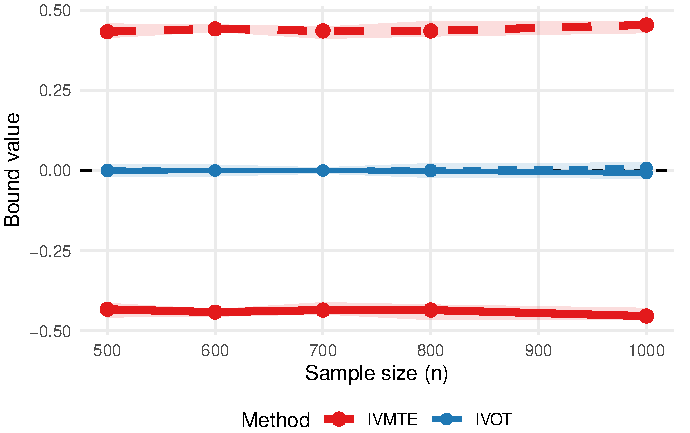
\includegraphics[width=0.75\linewidth]{figures/example3_1_bounds.pdf}
        \caption{Bounds of the moment relaxation approach and the CCOT approach by different sample sizes. Each data point is an average of 20 runs. In the experiment $M=1$, i.e., $y_{\max}=1, y_{\min}=-1$. }
        \label{fig:example3_1}
    \end{figure}
\end{example}

\section{Proofs of the Reduction Propositions}\label{oa:reductions}

This section proves the three closed-form rewritings on which the estimation procedures of \cref{sec:est_inf} are built. Each is an algebraic reduction of an expression already displayed in the main text, and none of the arguments below is used anywhere else.

\subsection{Proof of \cref{prop:discrete_reduction}}\label{app:closed_form_rewriting}

The nuisance components $\gamma_{\text{full},k}, \gamma_{j,k}, \gamma_K, J_{\text{full},k}, J_{j,k}, \Delta_K$ and the relative threshold $\kappa_{j,k}$ are defined in \cref{sec:est_inf} immediately preceding \cref{prop:discrete_reduction}; we refer to those formulas throughout this proof.

\begin{proof}[Proof of \cref{prop:discrete_reduction}]
    By \cref{thm:covariate_continuous_lower_bound} specialized to a finite instrument (every conditional LIV interval degenerate), it suffices to rewrite the conditional integral $\int_0^1 Q_{Y,k\mid X}(u)\,Q_{\omega,k\mid X}(1-u)\,\mathrm{d}u$ as an observable finite weighted sum. Fix $X$. On each baseline interval $(p_k(X), p_{k+1}(X))$ the weight function $\omega(X,u)$ is a non-increasing step function. On the sub-interval $(q_{j-1,k}(X),q_{j,k}(X))$, $j=1,\ldots,l_k$, exactly the current-bin instruments in $\bigcup_{l=j}^{l_k}T_{l,k}$ and all instruments whose alternative propensity lies in a strictly higher bin contribute to the first probability in $\omega$, whereas baseline propensities in strictly higher bins contribute to the second. Thus, up to the irrelevant boundary values,
    \begin{multline*}
        \omega(X,u) = \mathbb{P}_{\text{obs}}\!\left(Z \in \bigcup_{l=j}^{l_k} T_{l,k} \mathrel{\big|} X\right) + \mathbb{P}_{\text{obs}}\!\left(Z \in \bigcup_{i=k+1}^K \bigcup_{l=0}^{l_i} T_{l,i} \mathrel{\big|} X\right) \\
        - \mathbb{P}_{\text{obs}}\!\left(Z \in \bigcup_{i=k+1}^K S_i \mathrel{\big|} X\right),\quad u\in(q_{j-1,k},q_{j,k}).
    \end{multline*}
    Regrouping, the step-function value on the relevant slice is $\gamma_{\text{full},k}(X)+\gamma_{j,k}(X)$: the first term acts on the entire baseline interval and the second is the additional current-bin mass. Multiplying by $Q_{Y,k\mid X}$ and summing the nested current-bin contributions over the normalized sub-intervals yields
    \begin{multline*}
        (p_{k+1}(X) - p_k(X)) \int_0^1 Q_{Y,k\mid X}(u)\,Q_{\omega,k\mid X}(1-u)\,\mathrm{d}u \\
        = \gamma_{\text{full},k}(X)\, J_{\text{full},k}(X) + \sum_{j=1}^{l_k}\gamma_{j,k}(X)\, J_{j-1,k}(X),
    \end{multline*}
    where we used
    \begin{equation*}
        J_{\text{full},k}(X) = (p_{k+1}(X)-p_k(X))\,\mathbb{E}_{\mu_{1,k\mid X}}[Y] = (p_{k+1}(X)-p_k(X))\int_0^1 Q_{Y,k\mid X}(u)\,\mathrm{d}u
    \end{equation*}
    and the definition of $J_{j-1,k}$.

    The trivial-bound term on the tail $(p_K(X), 1]$ simplifies for the PRTE weight: since $\omega(X,u) = \mathbb{P}_{\text{obs}}(u < q(Z,X) \mid X) \geqslant 0$ for $u > p_K(X)$, we have $\int_{p_K(X)}^1 (y_{\min}\max\{0,\omega\} + y_{\max}\min\{0,\omega\})\,\mathrm{d}u = y_{\min}\int_{p_K(X)}^1 \omega(X,u)\,\mathrm{d}u$, which equals $\Delta_K(X)$ by Fubini. Taking the outer expectation over $X$ and summing over $k$ yields~(\ref{eq:target_discrete_iv}).

    The corresponding representation for the upper bound is obtained by the symmetric argument with $Q_{\omega,k\mid X}(1-t)$ replaced by $Q_{\omega,k\mid X}(t)$ in the OT term and $y_{\min}, y_{\max}$ swapped in the tail.
\end{proof}

\subsection{Proof of \cref{prop:J_specialization}}\label{app:J_specialization}

\begin{proof}[Proof of part (i).] Fix $k$ and $j \in \{0,\dots,l_k-1\}$. By the change of variables $u = F_{\mu_{1,k\mid X}}(y)$, continuity of $\mu_{1,k\mid X}$ at $\nu_{j,k}(X)$ and $\nu_{j+1,k}(X)$ gives $F_{\mu_{1,k\mid X}}(\nu_{j,k}(X)) = \kappa_{j,k}(X)$ and $F_{\mu_{1,k\mid X}}(\nu_{j+1,k}(X)) = \kappa_{j+1,k}(X)$ almost surely. Therefore,
\begin{align*}
    \int_{\kappa_{j,k}(X)}^{\kappa_{j+1,k}(X)} Q_{Y,k\mid X}(u)\,\mathrm{d}u &= \int_{\nu_{j,k}(X)}^{\nu_{j+1,k}(X)} y\, \mathrm{d}F_{\mu_{1,k\mid X}}(y) \\
    &= \mathbb{E}_{\mu_{1,k\mid X}}\!\big[Y\,\indicator\!\big(\nu_{j,k}(X) < Y \leqslant \nu_{j+1,k}(X)\big)\big],
\end{align*}
where the second equality uses the continuity of $\mu_{1,k\mid X}$ at the two boundary points to include/exclude boundary atoms without ambiguity. Multiplying by $p_{k+1}(X)-p_k(X)$ yields~(\ref{eq:J_cexpectation}).
\end{proof}

\begin{proof}[Proof of part (ii).] Suppose $Y \in \{0,1\}$. Let $\theta_k(X) \coloneqq \mathbb{E}_{\mu_{1,k\mid X}}[Y]$ denote the complier success probability on the $k$-th interval. By the definition of the identified complier measure \citep[cf.][]{angrist1995identification}, $(p_{k+1}(X)-p_k(X))\,\theta_k(X) = \mathbb{E}_{\text{obs}}[YW \mid Z \in S_{k+1}, X] - \mathbb{E}_{\text{obs}}[YW \mid Z \in S_k, X] = P_{1,k+1}(X) - P_{1,k}(X)$, so $J_{\text{full},k}(X) = P_{1,k+1}(X) - P_{1,k}(X)$.

Since $Y \in \{0,1\}$, the conditional quantile function is the step function $Q_{Y,k\mid X}(u) = \indicator(u \geqslant 1 - \theta_k(X))$. Equivalently, $Q_{Y,k\mid X}(u) = 1$ iff $u(p_{k+1}(X) - p_k(X)) + p_k(X) \geqslant p_{k+1}(X) - J_{\text{full},k}(X)$, i.e., the corresponding propensity value $v = p_k(X) + u(p_{k+1}(X)-p_k(X))$ lies in the interval $[p_{k+1}(X) - J_{\text{full},k}(X),\, p_{k+1}(X)]$. Writing $J_{j-1,k}(X)$ as a length in the original propensity scale, it equals the length of the intersection of $[q_{j-1,k}(X), q_{j,k}(X)]$ with $[p_{k+1}(X) - J_{\text{full},k}(X),\, p_{k+1}(X)]$:
\begin{equation*}
    J_{j-1,k}(X) = \max\!\Big(0,\; q_{j,k}(X) - \max\!\big(q_{j-1,k}(X),\; p_{k+1}(X) - J_{\text{full},k}(X)\big)\Big) = h_{j,k}^{-}(X).
\end{equation*}
Substituting into~(\ref{eq:target_discrete_iv}) yields~(\ref{eq:binary_lower_bound}).
\end{proof}

\subsection{Proof of \cref{prop:continuous_reduction}}\label{app:procedure_fubini}

\begin{proof}[Proof of \cref{prop:continuous_reduction}]
    Because $\mathcal{Z}$ is compact and connected and $z \mapsto p(z,X)$ is continuous by \cref{asp:continuity_p}, its image is a closed interval for almost every $X$, so \cref{thm:covariate_continuous_lower_bound} specializes with $K_X = 1$ and conditional LIV interval $[\underline{p}(X),\overline{p}(X)]$. We derive the three terms of~(\ref{eq:continuous_simplified_target}) in turn. Substituting the explicit form of the weight function,
    \begin{equation*}
        \omega(x,u) = \mathbb{E}_{Z \mid X}[\indicator (u \leqslant q(Z,X)) - \indicator (u \leqslant p(Z,X)) \mid X=x],
    \end{equation*}
    and applying Fubini's theorem to swap the order of integration, we handle each term separately.

    \textbf{First term (quantile integral on the gap $(0,\underline{p}(X))$).} For $\underline{p}(X)>0$, substitute the weight function, swap expectations, and use the change of variables $v=\underline{p}(X)u$. Because $P\ge \underline{p}(X)$ conditional on $X$, the baseline indicator equals one throughout this gap. Thus
    \begin{align*}
        \mathbb{E}_{X}&\!\left[ \underline{p}(X)\int_{0}^{1} Q_{1,\underline p\mid X}(u)\omega(X, \underline{p}(X)u)\, \mathrm{d}u \right] \\
        &= \mathbb{E}_{Z,X}\!\left[ \underline{p}(X)\int_{0}^{1} Q_{1,\underline p\mid X}(u)\big(\indicator (\underline{p}(X)u \leqslant q(Z,X)) - 1\big)\, \mathrm{d}u \right] \\
        &= -\mathbb{E}_{Z,X}\!\left[ \int_{\min\{\underline{p}(X),\,q(Z,X)\}}^{\underline{p}(X)} Q_{1,\underline p\mid X}\!\left({v}/{\underline{p}(X)}\right)\, \mathrm{d}v \right].
    \end{align*}
    Both sides are zero when $\underline{p}(X)=0$, which justifies the convention in the proposition.

    \textbf{Second term ($g_1$ difference on the LIV interval).} The structural integral representation gives $g_1(u,x)=\int_0^u\mathbb E[Y(1)\mid U=s,X=x]\,\mathrm ds$, so $g_1(\cdot,x)$ is absolutely continuous. Hence, for any $r\in[0,1]$,
    \[
        \int_{\underline{p}(X)}^{\overline{p}(X)} \partial_u g_1(u,X)\indicator(u\le r)\,\mathrm du
        =g_1\!\left(\min\{\overline{p}(X),\max\{\underline{p}(X),r\}\},X\right)-g_1(\underline{p}(X),X).
    \]
    Applying this identity first with $r=q(Z,X)$ and then with $r=P$ is essential when $q(Z,X)<\underline{p}(X)$. Since $P\in[\underline{p}(X),\overline{p}(X)]$, the two lower-endpoint terms cancel and give
    \begin{align*}
       \mathbb{E}_{X}\!\left[ \int_{\underline{p}(X)}^{\overline{p}(X)} \frac{\partial g_1(u, X)}{\partial u} \omega(X,u)\, \mathrm{d}u \right]
        &= \mathbb{E}_{Z,X}\!\left[g_1\big(q^{\mathrm{tr}}(Z,X),X\big)-g_1\big(P,X\big)\right].
    \end{align*}

    \textbf{Third term (trivial bound on $(\overline{p}(X),1]$).} Since $P\le \overline{p}(X)$, the baseline indicator vanishes on this tail and $\omega(X,u)=\mathbb P(u\le q(Z,X)\mid X)\ge0$. Therefore
    \begin{align*}
        y_{\min} \mathbb{E}_{X}\!\left[\int_{\overline{p}(X)}^{1} \omega(X,u)\, \mathrm{d}u\right]
        =y_{\min}\mathbb E_{Z,X}\!\left[(q(Z,X)-\overline{p}(X))_+\right].
    \end{align*}
    Aggregating the three components yields~(\ref{eq:continuous_simplified_target}). The upper-bound representation replaces the countermonotonic boundary coupling by the comonotonic coupling and swaps $y_{\min}$ for $y_{\max}$ in the trivial tail.
\end{proof}

\section{Moment Condition and Neyman Orthogonality of the Discrete-Instrument Scores}\label{oa:orthogonality}

This section proves \cref{lem:orthogonality_discrete}. Both parts are term-by-term calculations that repeatedly apply the tower property to inverse-probability-weighted residuals with zero conditional mean.

Throughout, $\eta_0$ denotes the vector of true nuisance parameter values and $\theta_0 = \underline{\theta}_{\omega,1}$ the true parameter value. For a functional $\Phi(\eta)$ and a perturbation direction $\delta$ in the same function space as $\eta$, we write $\partial_\delta \Phi(\eta) \coloneqq \frac{\mathrm{d}}{\mathrm{d}t}\Phi(\eta + t\,\delta)\big|_{t=0}$ for the Gateaux (directional) derivative; when the perturbation is along a single nuisance component $\eta_\alpha$, we write $\partial_{\eta_\alpha}$ for brevity.

\subsection{Continuous Outcome}\label{oa:orthogonality_continuous}

Recall the target functional:
\begin{equation}\label{eq:pf_target_recall}
    \theta_0 = \mathbb{E}\Bigg[\sum_{k=0}^{K-1}\bigg(\gamma_{\mathrm{full},k}(X)\,J_{\mathrm{full},k}(X) + \sum_{j=1}^{l_k} \gamma_{j,k}(X)\,J_{j-1,k}(X)\bigg) + \Delta_K(X)\Bigg],
\end{equation}
and the total Neyman-orthogonal score assembled from the components of \cref{app:scores_continuous}:
\begin{equation}\label{eq:pf_total_score}
    \psi(O;\eta) = \sum_{k=0}^{K-1}\Bigl(\psi_{\mathrm{full},k}^{\mathrm{prod}}(O;\eta) + \sum_{j=1}^{l_k}\psi_{j,k}^{\mathrm{prod}}(O;\eta)\Bigr) + \psi_{\Delta_K}(O;\eta),
\end{equation}
where each product score debiases the corresponding term in the target. Specifically, $\psi_{j,k}^J(O;\eta)$ is the uncentered orthogonal score for the conditional integral component $\mathbb{E}[J_{j,k}(X)]$, and the product score for $\mathbb{E}[\gamma_{j,k}(X)\,J_{j-1,k}(X)]$ is:
\begin{equation}\label{eq:pf_prod_score_recall}
    \psi_{j,k}^{\mathrm{prod}}(O;\eta) = \gamma_{j,k}(X)\,\psi_{j-1,k}^J(O;\eta) + J_{j-1,k}(X)\Bigl(\indicator\bigl(Z \in {\textstyle\bigcup_{l=j}^{l_k}} T_{l,k}\bigr) - \gamma_{j,k}(X)\Bigr),
\end{equation}
and symmetrically for $\psi_{\mathrm{full},k}^{\mathrm{prod}}(O;\eta)$.

\begin{proof}[Proof of \cref{lem:orthogonality_discrete}\textup{(i)}]
\medskip
\noindent\textbf{Moment condition.}
We show $\mathbb{E}[\psi(O;\eta_0)] = \theta_0$. All influence function correction terms in the score are inverse-probability-weighted residuals of the general form
\[
    \frac{\indicator(Z \in S_k)}{\pi_k(X)}\,W\bigl(g(Y,X) - \mathbb{E}[g(Y,X) \mid X, Z \in S_k, W\!=\!1]\bigr).
\]
By the tower property, conditioning first on $(X,Z)$: when $Z \in S_k$, we have $p(Z,X) = p_k(X)$, so $\mathbb{E}[W \mid X, Z \in S_k] = p_k(X)$. It follows that
\[
    \mathbb{E}\Big[\frac{\indicator(Z \in S_k)}{\pi_k(X)}\,W\bigl(g - \mathbb{E}[g \mid X, S_k, W\!=\!1]\bigr)\Big] = \mathbb{E}\Big[\frac{\indicator(Z \in S_k)}{\pi_k(X)}\,p_k(X)\cdot 0\Big] = 0.
\]
Applying this identity to each correction term, $\mathbb{E}[IF_{J^\pm}(O)] = 0$ and $\mathbb{E}[IF_{M_{j,k}^\pm}(O)] = 0$ at $\eta_0$. The quantile correction term in $\psi_{j,k}^J$ contains the factor $p_{k+1}(X)M_{j,k}^+(X) - p_k(X)M_{j,k}^-(X) - (q_{j,k}(X) - p_k(X))$, which vanishes at $\eta_0$ by the conditional moment equation
\begin{equation}\label{eq:pf_quantile_moment_dml}
    \begin{split}
        &p_{k+1}(X)\,\mathbb{E}[\indicator(Y \leqslant \nu_{j,k}(X)) \mid X, S_{k+1}, W\!=\!1]\\
        & \quad\quad \quad \quad - p_k(X)\,\mathbb{E}[\indicator(Y \leqslant \nu_{j,k}(X)) \mid X, S_k, W\!=\!1] - (q_{j,k}(X) - p_k(X)) = 0
    \end{split}
\end{equation}
which defines $\nu_{j,k}$ for $j\geqslant1$; the boundary value $\nu_{0,k}=y_{\min}$ is fixed. The propensity score correction terms $\frac{\indicator(Z \in S_k)}{\pi_k(X)}(W - p_k(X))$ and the pooled policy-level residuals $R_{q,j,k}$ likewise have zero mean by the same tower-property argument. Consequently,
\begin{align*}
    \mathbb{E}[\psi_{j,k}^J(O;\eta_0)] &= \mathbb{E}[J_{j,k}(X)], & \mathbb{E}[\psi_{\mathrm{full},k}^J(O;\eta_0)] &= \mathbb{E}[J_{\mathrm{full},k}(X)].
\end{align*}
For the product scores, substituting~(\ref{eq:pf_prod_score_recall}) and using $\mathbb{E}[\indicator(Z \in \bigcup_{l=j}^{l_k} T_{l,k}) - \gamma_{j,k}(X)] = 0$:
\begin{align*}
    \mathbb{E}[\psi_{j,k}^{\mathrm{prod}}(O;\eta_0)] &= \mathbb{E}\bigl[\gamma_{j,k}(X)\,\underbrace{\mathbb{E}[\psi_{j-1,k}^J(O;\eta_0) \mid X]}_{= J_{j-1,k}(X)}\bigr] + \mathbb{E}\bigl[J_{j-1,k}(X)\,\underbrace{\mathbb{E}[\indicator(\cdots) - \gamma_{j,k}(X) \mid X]}_{= 0}\bigr] \\
    &= \mathbb{E}[\gamma_{j,k}(X)\,J_{j-1,k}(X)],
\end{align*}
and symmetrically $\mathbb{E}[\psi_{\mathrm{full},k}^{\mathrm{prod}}(O;\eta_0)] = \mathbb{E}[\gamma_{\mathrm{full},k}(X)\,J_{\mathrm{full},k}(X)]$. The same reasoning yields $\mathbb{E}[\psi_{\Delta_K}(O;\eta_0)] = \mathbb{E}[\Delta_K(X)]$. Summing over all components and comparing with~(\ref{eq:pf_target_recall}) gives $\mathbb{E}[\psi(O;\eta_0)] = \theta_0$.

\medskip
\noindent\textbf{Neyman orthogonality of $\psi_{j,k}^J$.}
We show that the Gateaux derivative $\partial_t\,\mathbb{E}[\psi_{j,k}^J(O;\eta_0 + t\,\delta)]|_{t=0}$ vanishes for all perturbation directions~$\delta$. We group the nuisance parameters by type and check orthogonality with respect to each group.

\textbf{Conditional expectations $(J_{j,k}^\pm, M_{j,k}^\pm)$.}
Consider a perturbation $J_{j,k}^+(X) \to J_{j,k}^+(X) + t\,\delta J^+(X)$. The plug-in term $J_{j,k} = p_{k+1}\,J_{j,k}^+ - p_k\,J_{j,k}^-$ contributes $+\mathbb{E}[p_{k+1}(X)\,\delta J^+(X)]$, while the IPW correction $IF_{J^+}$ contributes $-\mathbb{E}\bigl[\frac{\indicator(Z \in S_{k+1})}{\pi_{k+1}(X)}\,p_{k+1}(X)\,\delta J^+(X)\bigr]$. These cancel because
\[
    \mathbb{E}\!\left[\frac{\indicator(Z \in S_{k+1})}{\pi_{k+1}(X)} \mathrel{\bigg|} X\right] = \frac{\mathbb{P}(Z \in S_{k+1} \mid X)}{\pi_{k+1}(X)} = 1.
\]
For $J_{j,k}^-$ the plug-in derivative is $-p_k\delta J^-$, while differentiating $-IF_{J^-}$ gives $+p_k\delta J^-$. For $M_{j,k}^+$, the plug-in part of the quantile moment gives $\nu_{j,k}p_{k+1}\delta M^+$ and differentiating $\nu_{j,k}IF_{M_{j,k}^+}$ gives its negative; the minus-side and $j+1$ terms cancel in the same way, with their displayed signs. Thus every conditional-expectation direction cancels explicitly.

\textbf{Instrument assignment probabilities $(\pi_k, \pi_{k+1})$.}
Perturbing $\pi_{k+1}(X) \to \pi_{k+1}(X) + t\,\delta\pi(X)$ introduces a factor $-\delta\pi(X)/\pi_{k+1}(X)^2$ in the IPW terms. For any such IPW term $\indicator(Z \in S_{k+1})\,\pi_{k+1}(X)^{-1}\,W\,(g(O) - \bar{g}(X))$, the first-order contribution is
\[
    -\mathbb{E}\!\left[\frac{\indicator(Z \in S_{k+1})}{\pi_{k+1}(X)^2}\,\delta\pi(X)\,W\,(g(O) - \bar{g}(X))\right].
\]
Conditioning on $(X,Z)$ with $Z \in S_{k+1}$, we have $\mathbb{E}[W(g(O) - \bar{g}(X)) \mid X, Z \in S_{k+1}] = p_{k+1}(X) \cdot 0 = 0$ at $\eta_0$, so the Gateaux derivative vanishes. The argument for $\delta\pi_k$ is identical when $k\geqslant1$; there is no $\pi_0$ direction.

\textbf{Propensity scores $(p_k, p_{k+1})$.}
For $k\geqslant1$, a perturbation $p_k(X) \to p_k(X) + t\,\delta p_k(X)$ generates first-order contributions from three sources (all multiplied by $\delta p_k(X)$ inside $\mathbb{E}[\cdot]$). There is no such direction at $k=0$ because $p_0\equiv0$ is fixed:
\begin{enumerate}
    \item[(i)] The plug-in term $J_{j,k} = p_{k+1}\,J_{j,k}^+ - p_k\,J_{j,k}^-$, contributing $-J_{j,k}^-(X)$;
    \item[(ii)] The quantile correction terms $\nu_{j,k}(\cdots) - \nu_{j+1,k}(\cdots)$, contributing $\nu_{j,k}(X)(\indicator(j\geqslant1) - M_{j,k}^-(X)) - \nu_{j+1,k}(X)(1 - M_{j+1,k}^-(X))$. At $j=0$, the first constant is absent because $q_{0,k}-p_k\equiv0$;
    \item[(iii)] The Riesz representer correction $\alpha_{p_k}(X)\frac{\indicator(Z \in S_k)}{\pi_k(X)}(W - p_k(X))$, contributing $-\alpha_{p_k}(X)$.
\end{enumerate}
Substituting the definition
\[
    \alpha_{p_k} = -J_{j,k}^- - \nu_{j,k}\,M_{j,k}^- + \nu_{j+1,k}\,M_{j+1,k}^- + \indicator(j\geqslant1)\nu_{j,k} - \nu_{j+1,k}
\]
and collecting terms:
\begin{align*}
    &\bigl(-J_{j,k}^-\bigr) + \bigl(\indicator(j\geqslant1)\nu_{j,k} - \nu_{j,k}\,M_{j,k}^- - \nu_{j+1,k} + \nu_{j+1,k}\,M_{j+1,k}^-\bigr) \\
    &\quad - \bigl(-J_{j,k}^- - \nu_{j,k}\,M_{j,k}^- + \nu_{j+1,k}\,M_{j+1,k}^- + \indicator(j\geqslant1)\nu_{j,k} - \nu_{j+1,k}\bigr) = 0.
\end{align*}
The calculation for $\delta p_{k+1}$, using $\alpha_{p_{k+1}} = J_{j,k}^+ + \nu_{j,k}\,M_{j,k}^+ - \nu_{j+1,k}\,M_{j+1,k}^+$, is identical.

\textbf{Quantile thresholds $(\nu_{j,k}, \nu_{j+1,k})$.}
A perturbation is considered only for estimated thresholds. In particular, $\nu_{0,k}=y_{\min}$ is fixed and has no nuisance direction.
A perturbation $\nu_{j,k}(X) \to \nu_{j,k}(X) + t\,\delta\nu(X)$ affects the score through two channels.

\textbf{Channel~(a): indicator boundaries.} The indicator $\indicator(\nu_{j,k}(X) \leqslant Y)$ appears inside $IF_{J^\pm}$ and $IF_{M_{j,k}^\pm}$. For a generic relevant conditional law $F$ and $a_t=\nu+t\,\delta\nu$, the combined boundary change from the truncated first-moment correction and its quantile-moment correction is, up to its orientation,
\[
    \int_{\nu}^{a_t}(a_t-y)\,\mathrm{d}F(y).
\]
If the density of $F$ is bounded by $C$ in the stated neighborhood, then
\[
    \left|\int_{\nu}^{a_t}(a_t-y)\,\mathrm{d}F(y)\right|
    \leqslant C|a_t-\nu|^2.
\]
The oriented-integral convention covers $a_t<\nu$. Applying this bound to the plus and minus conditional laws shows that the combined boundary contribution is $O(t^2\delta\nu^2)$ and therefore has derivative zero at $t=0$.

\textbf{Channel~(b): explicit multiplicative factor.} The term $\nu_{j,k}(X)\bigl(p_{k+1} M_{j,k}^+ - p_k M_{j,k}^- - (q_{j,k} - p_k)\bigr)$ contributes $\delta\nu(X)$ times the conditional moment equation~(\ref{eq:pf_quantile_moment_dml}), which vanishes at $\eta_0$. The dependence of $\alpha_{p_k}$ and $\alpha_{p_{k+1}}$ on $\nu_{j,k}$ is absorbed by the zero-mean residuals: for any $L_2$ function $h(X)$,
\[
    \mathbb{E}\!\left[h(X)\,\frac{\indicator(Z \in S_k)}{\pi_k(X)}\bigl(W - p_k(X)\bigr)\right] = \mathbb{E}\!\left[h(X)\,\frac{\pi_k(X)}{\pi_k(X)}\cdot 0\right] = 0.
\]
The local density bound gives the quadratic control above. The treatment of $\delta\nu_{j+1,k}$ is symmetric.

\textbf{Alternative policy propensity $(q_{j,k})$.}
For $j\geqslant1$, use the pooled representation $q_{j,k}(X)=\mathbb E[q(Z,X)\mid Z\in T_{j,k},X]$. At the population law, all the instrument-specific policy propensities in $T_{j,k}$ equal this common value. Consequently, perturbations of the conditional instrument probabilities have no first-order effect on the pooled value, while perturbing the propensity functions induces
\[
    \delta q_{j,k}(X)
    =\frac{1}{\tau_{j,k}(X)}
      \sum_{z\in T_{j,k}}\pi(z,X)
      \frac{\partial\phi}{\partial p}(z,X,p(z,X))\,\delta p(z,X).
\]
At $j=0$, $T_{0,k}=\emptyset$ and the boundary $q_{0,k}=p_k$ is handled by the corrected $p_k$ representer above. For $j\geqslant1$, the first-order contributions are:
\begin{align*}
    \text{from quantile correction}&: \quad -\mathbb{E}\bigl[\nu_{j,k}(X)\,\delta q_{j,k}(X)\bigr], \\
    \text{from differentiating the policy residual}&: \quad +\mathbb{E}\bigl[\nu_{j,k}(X)\,\delta q_{j,k}(X)\bigr].
\end{align*}
The pooled correction itself has mean zero at the truth. Differentiating its residuals gives
\[
    \partial_t\mathbb E[-\nu_{j,k}(X)R_{q,j,k}(O)]\big|_{t=0}
    =\mathbb E[\nu_{j,k}(X)\,\delta q_{j,k}(X)],
\]
because $\mathbb E[\indicator(Z=z)\mid X]=\pi(z,X)$. Derivatives of the coefficients multiply zero-mean residuals and therefore vanish. The two displayed contributions cancel, and the treatment of $q_{j+1,k}$ is symmetric.

The simplex restriction is essential for the preceding pooled representation. Along a within-set share perturbation $a_{j,k}(z,X)\mapsto a_{j,k}(z,X)+t\,\delta a_z(X)$, admissible directions satisfy $\sum_{z\in T_{j,k}}\delta a_z(X)=0$. Since $q(z,X)=q_{j,k}(X)$ for every $z\in T_{j,k}$ at the population law,
\[
    \partial_t\sum_{z\in T_{j,k}}(a_{j,k}(z,X)+t\,\delta a_z(X))q(z,X)\Big|_{t=0}
    =q_{j,k}(X)\sum_{z\in T_{j,k}}\delta a_z(X)=0.
\]
With estimated instrument-specific policy values, the remaining share term is $\sum_z(\hat a_z-a_z)(\hat q(z,X)-q_{j,k}(X))$, a product of two nuisance errors. A perturbation of $\tau_{j,k}$ affects only the factor $1/\tau_{j,k}$ in $R_{q,j,k}$; its derivative multiplies the conditionally mean-zero numerator $\sum_{z\in T_{j,k}}\phi_p(z,X,p(z,X))\indicator(Z=z)(W-p(z,X))$ and is therefore zero at the truth.

This establishes orthogonality for $\psi_{j,k}^J$.

\medskip
\noindent\textbf{Neyman orthogonality of the remaining components.}
For $\psi_{\mathrm{full},k}^J$, a perturbation of $J_{\mathrm{full},k}^+$ contributes $p_{k+1}\delta J^+$ through the plug-in and $-p_{k+1}\delta J^+$ through its outcome residual. A perturbation of $p_{k+1}$ contributes $J_{\mathrm{full},k}^+\delta p_{k+1}$ through the plug-in and its negative through the propensity residual. The minus-side terms cancel identically when $k\geqslant1$, and denominator perturbations in $\pi_k,\pi_{k+1}$ multiply conditionally mean-zero residuals. Hence $\psi_{\mathrm{full},k}^J$ is orthogonal in every nuisance direction.

For the product scores, we invoke the chain rule for influence functions. The preceding cancellations hold conditionally on $X$: at $\eta_0$, $\mathbb E[\psi_{j-1,k}^J(O;\eta_0)\mid X]=J_{j-1,k}(X)$, and the Gateaux derivative of this conditional moment is zero in every nuisance direction already considered. Moreover, $\indicator(Z \in \bigcup_{l=j}^{l_k} T_{l,k}) - \gamma_{j,k}(X)$ is the conditional influence function for $\gamma_{j,k}(X) = \mathbb{P}(Z \in \bigcup_{l=j}^{l_k} T_{l,k} \mid X)$. Therefore, the product score~(\ref{eq:pf_prod_score_recall})
\[
    \psi_{j,k}^{\mathrm{prod}} = \gamma_{j,k}(X)\,\psi_{j-1,k}^J(O;\eta) + J_{j-1,k}(X)\bigl(\indicator(Z \in {\textstyle\bigcup_{l=j}^{l_k}} T_{l,k}) - \gamma_{j,k}(X)\bigr)
\]
is orthogonal for the product functional $\mathbb{E}[\gamma_{j,k}(X)\,J_{j-1,k}(X)]$. We treat the two groups of nuisance directions separately. First, let $\eta_\alpha$ be any component other than $\gamma_{j,k}$. Then $\gamma_{j,k}$ and the indicator residual do not vary, so
\begin{multline*}
    \partial_{\eta_\alpha}\mathbb{E}[\psi_{j,k}^{\mathrm{prod}}] = \mathbb{E}\bigl[\gamma_{j,k}(X)\,\underbrace{\partial_{\eta_\alpha}\mathbb{E}[\psi_{j-1,k}^J \mid X]}_{=\,0}\bigr] \\
    + \mathbb{E}\bigl[\partial_{\eta_\alpha}J_{j-1,k}(X)\,\underbrace{\mathbb{E}[\indicator(\cdots) - \gamma_{j,k}(X) \mid X]}_{=\,0}\bigr] = 0,
\end{multline*}
where the first expectation vanishes by the conditional orthogonality just established. Second, for the direction $\gamma_{j,k} \mapsto \gamma_{j,k} + t\,\delta\gamma$, the derivative contributions of the explicit prefactor and the residual cancel:
\[
    \partial_t\,\mathbb{E}\bigl[(\gamma_{j,k}+t\,\delta\gamma)\psi_{j-1,k}^J + J_{j-1,k}(\indicator(\cdots) - \gamma_{j,k} - t\,\delta\gamma)\bigr]\Big|_{t=0}
    = \mathbb{E}[\delta\gamma\,J_{j-1,k}] - \mathbb{E}[\delta\gamma\,J_{j-1,k}] = 0,
\]
using $\mathbb{E}[\psi_{j-1,k}^J \mid X] = J_{j-1,k}(X)$ at $\eta_0$. For the full-interval product, the residual is
\[
\indicator\!\left(Z\in\bigcup_{m=k+1}^K\bigcup_{l=0}^{l_m}T_{l,m}\right)
-\indicator\!\left(Z\in\bigcup_{m=k+1}^KS_m\right)-\gamma_{\mathrm{full},k}(X),
\]
whose conditional mean is zero by the definition of $\gamma_{\mathrm{full},k}$. Therefore its coefficient and residual derivatives cancel exactly as in~(\ref{eq:pf_prod_score_recall}), even though $\gamma_{\mathrm{full},k}$ is signed.

For $\psi_{\Delta_K}$, write
\begin{equation*}
    A_K=\Bigl\{Z\in\bigcup\nolimits_{j=1}^{l_K}T_{j,K}\Bigr\}.
\end{equation*}
A perturbation of $p_K$ contributes $-y_{\min}\mathbb E[\gamma_K(X)\,\delta p_K(X)]$ through the plug-in term and the opposite quantity through differentiation of the $p_K$ residual. For an instrument-specific direction $p(z,X)\mapsto p(z,X)+t\,\delta p(z,X)$, the plug-in derivative is
\[
y_{\min}\mathbb E\!\left[\indicator(A_K)\phi_p(Z,X,p(Z,X))\delta p(Z,X)\right],
\]
and differentiation of the policy residual gives its negative. Perturbations of $\pi_K$ and of the coefficient $\gamma_K$ multiply the conditionally mean-zero $p_K$ residual, while derivatives of $\phi_p$ multiply $W-p(Z,X)$ and also have conditional mean zero. Thus every first-order direction in $\psi_{\Delta_K}$ cancels.

\end{proof}

\subsection{Binary Outcome}\label{oa:orthogonality_binary}

\begin{proof}[Proof of \cref{lem:orthogonality_discrete}\textup{(ii)}]
Recall the target functional~(\ref{eq:binary_lower_bound}) and the orthogonal score~(\ref{eq:binary_score}), which decomposes as $\psi = \sum_{k}(\psi_{\mathrm{full},k}^{\mathrm{prod}} + \sum_{j}\psi_{j,k}^{\mathrm{prod}}) + \psi_{\Delta_K}$.
\medskip
\noindent\textbf{Moment condition.}
We show $\mathbb{E}[\psi(O;\eta_0)] = \theta_0$. The residuals $R_{P,k}$ and $R_{p,k}$ have conditional mean zero because $P_{1,k}(X)=\mathbb E[YW\mid Z\in S_k,X]$ and $p_k(X)=\mathbb E[W\mid Z\in S_k,X]$. The pooled policy residual also satisfies
\begin{multline*}
\mathbb E[R_{q,j,k}(O)\mid X] \\
=\frac1{\tau_{j,k}(X)}\sum_{z\in T_{j,k}}\phi_p(z,X,p(z,X))\,\mathbb P(Z=z\mid X)\,\mathbb E[W-p(z,X)\mid Z=z,X]
=0.
\end{multline*}
Thus every correction in $\psi_{j,k}^h$ and $\psi_{\mathrm{full},k}^J$ has conditional mean zero, so $\mathbb{E}[\psi_{j,k}^h(O;\eta_0)\mid X] = h_{j,k}^-(X)$ and $\mathbb{E}[\psi_{\mathrm{full},k}^J(O;\eta_0)\mid X] = J_{\mathrm{full},k}(X)$. Writing $A_{j,k}=\{Z\in\bigcup_{l=j}^{l_k}T_{l,k}\}$, another application of the tower property gives
\begin{align*}
    \mathbb E[\psi_{j,k}^{\mathrm{prod}}(O;\eta_0)]
    &=\mathbb E\!\left[\gamma_{j,k}(X)\,\mathbb E[\psi_{j,k}^h(O;\eta_0)\mid X]
      +h_{j,k}^-(X)\,\mathbb E[\indicator(A_{j,k})-\gamma_{j,k}(X)\mid X]\right] \\
    &=\mathbb E[\gamma_{j,k}(X)h_{j,k}^-(X)].
\end{align*}
The same conditional calculation applies to the full-interval product score. Summing all components therefore gives $\mathbb{E}[\psi(O;\eta_0)] = \mathbb{E}[m(X;\eta_0)] = \theta_0$.

\medskip
\noindent\textbf{Neyman orthogonality.}
We must show $\partial_{\eta_\alpha}\mathbb{E}[\psi(O;\eta)]\big|_{\eta=\eta_0} = 0$ for each nuisance component $\eta_\alpha$. By the product score structure, it suffices to establish orthogonality of the component scores $\psi_{j,k}^h$ and $\psi_{\mathrm{full},k}^J$ with respect to $(P_{1,m},p_m,p(z,X),\pi_m,\tau_{j,k},a_{j,k})$, and then show that the product scores inherit orthogonality with respect to the $\gamma$ terms.

\textbf{Orthogonality of $\psi_{j,k}^h$ with respect to $P_{1,m}$.}
Consider a perturbation $P_{1,m} \to P_{1,m} + t\,\delta P_{1,m}(X)$. Since $h_{j,k}^-$ depends on $P_{1,m}$ only through $J_{\mathrm{full},k} = P_{1,k+1} - P_{1,k}$, the pathwise derivative is
\[
    \partial_t \mathbb{E}[h_{j,k}^-] \big|_{t=0} = \mathbb{E}\!\left[\alpha_{P,m}^{(j,k)}(X)\,\delta P_{1,m}(X)\right],
\]
where $\alpha_{P,k+1}^{(j,k)} = D_{j,k}^-$, $\alpha_{P,k}^{(j,k)} = -D_{j,k}^-$, and $\alpha_{P,m}^{(j,k)} = 0$ for $m \notin \{k,k{+}1\}$. Under \cref{asp:discrete_outcome_gap}, $D_{j,k}^- = \indicator(q_{j-1,k} < p_{k+1} - J_{\mathrm{full},k} < q_{j,k})$ is well-defined. The IPW correction $D_{j,k}^-(R_{P,k+1} - R_{P,k})$ in $\psi_{j,k}^h$ contributes
\begin{multline*}
    \partial_t \mathbb{E}\!\left[D_{j,k}^-\!\left(\frac{\indicator(Z \in S_{k+1})}{\pi_{k+1}}\bigl(YW - P_{1,k+1}\bigr) - \frac{\indicator(Z \in S_k)}{\pi_k}\bigl(YW - P_{1,k}\bigr)\right)\right]\bigg|_{t=0} \\
    = -\mathbb{E}\!\left[\alpha_{P,m}^{(j,k)}\,\delta P_{1,m}\right],
\end{multline*}
using $\mathbb{E}[\frac{\indicator(Z \in S_m)}{\pi_m} \mid X] = 1$, so the two contributions cancel. The same argument gives $\partial_{P_{1,m}}\mathbb{E}[\psi_{\mathrm{full},k}^J] = 0$ (with $\alpha_{P,k+1}^{(\mathrm{full},k)} = 1$ and $\alpha_{P,k}^{(\mathrm{full},k)} = -1$).

\noindent\textit{Remark (notation).} For $k\in\{0,\ldots,K-1\}$ and $j\in\{1,\ldots,l_k\}$, $\alpha_{P,k}^{(j,k)}(x)=-D_{j,k}^{-}(x)$ is the coefficient of the $P_{1,k}$ perturbation in the derivative of $h_{j,k}^{-}$, with the other nuisance arguments held fixed.


\textbf{Orthogonality of $\psi_{j,k}^h$ with respect to $p_m$ and $p(z,X)$.}
The propensity scores enter $h_{j,k}^-$ through three channels:

\begin{enumerate}[label=(\alph*)]
    \item the integration boundary $p_{k+1} - J_{\mathrm{full},k}$, corrected by $\alpha_{p,k+1}^{(j,k)} R_{p,k+1}$;
    \item the lower level-set boundary $q_{0,k} = p_k$ when $j = 1$, corrected by $\alpha_{p,k}^{(1,k)} R_{p,k}$;
    \item the alternative policy values $q_{j,k}$ and $q_{j-1,k}$ through the mapping $\phi(z,X,p(z,X))$, corrected by the policy terms involving $T_{j,k}$ and $T_{j-1,k}$.
\end{enumerate}

For channel (a), a perturbation $p_{k+1} \to p_{k+1} + t\,\delta p_{k+1}(X)$ shifts the boundary by $\delta p_{k+1}$, giving $\partial_t h_{j,k}^- = -D_{j,k}^-\,\delta p_{k+1}$. The correction $\alpha_{p,k+1}^{(j,k)} R_{p,k+1} = -D_{j,k}^- \cdot \frac{\indicator(Z \in S_{k+1})}{\pi_{k+1}}(W - p_{k+1})$ contributes $\partial_t \mathbb{E}[\alpha_{p,k+1}^{(j,k)} R_{p,k+1}] = D_{j,k}^-\,\delta p_{k+1}$, canceling the plug-in derivative.

For channel (b), when $j = 1$ and $E_{1,k}^- = 1$ (i.e., $p_k > p_{k+1} - J_{\mathrm{full},k}$), a perturbation of $p_k$ shifts $q_{0,k} = p_k$, giving $\partial_t h_{1,k}^- = -E_{1,k}^- I_{1,k}^-\,\delta p_k$. The correction $\alpha_{p,k}^{(1,k)} R_{p,k}$ contributes the matching cancellation.

For channel (c), the pooled derivative displayed in the continuous-outcome proof gives $\partial_t h_{j,k}^-=I_{j,k}^-\,\delta q_{j,k}$ for the upper boundary. The derivative of $I_{j,k}^-R_{q,j,k}$ is $-I_{j,k}^-\,\delta q_{j,k}$ and therefore cancels it. Symmetrically, when $E_{j,k}^-=1$, the correction through $R_{q,j-1,k}$ cancels the derivative through the lower boundary $q_{j-1,k}$.

\textbf{Denominators and within-set shares.}
A perturbation of $\pi_m$ differentiates only denominators in $R_{P,m}$ and $R_{p,m}$; each resulting term is a function of $X$ times a conditionally mean-zero residual, so its expectation is zero. The same argument applies to a perturbation of $\tau_{j,k}$ in $R_{q,j,k}$. Finally, admissible share directions satisfy $\sum_{z\in T_{j,k}}\delta a_z(X)=0$. At the truth, all $q(z,X)$ in $T_{j,k}$ equal $q_{j,k}(X)$, and hence
\[
\partial_t\sum_{z\in T_{j,k}}(a_{j,k}(z,X)+t\delta a_z(X))q(z,X)\Big|_{t=0}
=q_{j,k}(X)\sum_{z\in T_{j,k}}\delta a_z(X)=0.
\]
Thus the simplex-share direction has no first-order effect; with estimated $q(z,X)$ it contributes only the product $\sum_z(\hat a_z-a_z)(\hat q_z-q_{j,k})$.

\textbf{Inheritance by product scores.}
Recall that
\begin{equation*}
    \psi_{j,k}^{\mathrm{prod}} = \gamma_{j,k}\,\psi_{j,k}^h + h_{j,k}^-(\indicator(\cdots) - \gamma_{j,k}),
    \qquad \mathbb{E}[\indicator(\cdots) - \gamma_{j,k} \mid X] = 0 \ \text{ at } \eta_0,
\end{equation*}
while the preceding component-score cancellations hold conditionally on $X$. Hence any perturbation of a component-score nuisance
$(P_{1,m},\,p_m,\,p(z,X),\,\pi_m,\,\tau_{j,k},\,a_{j,k})$
yields
\[
    \partial_\eta \mathbb{E}[\psi_{j,k}^{\mathrm{prod}}]
    =\mathbb E\!\left[\gamma_{j,k}(X)\,\underbrace{\partial_\eta \mathbb{E}[\psi_{j,k}^h\mid X]}_{=\,0}
    +\partial_\eta h_{j,k}^-(X)\,\underbrace{\mathbb{E}[\indicator(\cdots) - \gamma_{j,k}(X) \mid X]}_{=\,0}\right]=0.
\]
For $\psi_{\mathrm{full},k}^{\mathrm{prod}}$, the same calculation uses the signed residual
\[
\indicator\!\left(Z\in\bigcup_{m=k+1}^K\bigcup_{l=0}^{l_m}T_{l,m}\right)
-\indicator\!\left(Z\in\bigcup_{m=k+1}^KS_m\right)-\gamma_{\mathrm{full},k}(X),
\]
whose conditional mean is zero. For $\psi_{\Delta_K}$, the $p_K$ plug-in derivative cancels the derivative of its $R_{p,K}$ correction, while each instrument-specific derivative through $q(z,X)=\phi(z,X,p(z,X))$ cancels the corresponding policy residual. Perturbations of $\pi_K$, $\gamma_K$, and the policy-derivative coefficient multiply conditionally mean-zero residuals. Hence $\psi_{\Delta_K}$ is also orthogonal in every nuisance direction.

\textbf{Perturbation of $\gamma_{j,k}$ and $\gamma_{\mathrm{full},k}$.}
The derivative contributions of the two product-score terms cancel. Along $\gamma_{j,k} \mapsto \gamma_{j,k} + t\,\delta\gamma$,
\[
    \partial_t\,\mathbb{E}\bigl[(\gamma_{j,k}+t\,\delta\gamma)\,\psi_{j,k}^h + h_{j,k}^-\bigl(\indicator(\cdots) - \gamma_{j,k} - t\,\delta\gamma\bigr)\bigr]\Big|_{t=0}
    = \mathbb{E}\bigl[\delta\gamma\,\mathbb{E}[\psi_{j,k}^h \mid X]\bigr] - \mathbb{E}\bigl[\delta\gamma\,h_{j,k}^-\bigr] = 0,
\]
because $\mathbb{E}[\psi_{j,k}^h \mid X] = h_{j,k}^-(X)$ at $\eta_0$. Replacing the set-indicator residual by the signed residual displayed above gives the identical cancellation for $\gamma_{\mathrm{full},k}$.

\end{proof}

\section{Rate and Learner Conditions for the Concrete Continuous-Instrument Estimator}\label{app:continuous_learner_conditions}

\cref{thm:continuous_rate} accepts any nuisance construction satisfying its three target losses. We now express those losses in terms of the learner prediction errors for \cref{alg:continuous_instrument}, stated in \cref{app:continuous_concrete} of \supplocation. \cref{asp:continuous_learners} uses the following quantities:
\begin{itemize}
    \item[--] $r_{p,n}$, a sup-norm first-stage rate, $\|\hat p-p\|_\infty=O_P(r_{p,n})$;
    \item[--] $r_{g,\mathrm{loc},n}$, an $L_1$ prediction rate for $\hat g_1$, required only at the two arguments $\hat q^{\mathrm{tr}}(Z,X)$ and $\hat P$ at which the target evaluates it;
    \item[--] $r_{Q,n}$, a $\underline p(X)$-weighted $L_1$ rate for the conditional quantile fit relative to the law generated by the estimated boundary window, and $\varepsilon_n$, the width of the two analytically trimmed quantile tails;
    \item[--] $\delta_n+r_{p,n}$, the structural distance between that selected law and the canonical treated boundary law.
\end{itemize}
The first stage remains uniform because $\hat p$ determines conditional support extrema and membership in the shrinking boundary sample in addition to serving as a generated regressor. The same uniform first-stage requirement arises in nonparametric problems with generated covariates; see, for example, \citet[Assumption 2]{mammen_rothe_schienle2012} and \citet[Assumption 7]{lee2018partial_mean}.

\begin{corollary}[Rate for the Concrete Estimator]\label{cor:continuous_primitive_rate}
    Suppose \cref{asp:structure} and \cref{asp:continuity_p} hold. Suppose additionally that $\phi$ is uniformly Lipschitz in its last argument: for some $L_\phi<\infty$,
    \[
        |\phi(z,x,p')-\phi(z,x,p)|\leqslant L_\phi|p'-p|
    \]
    for all $(z,x,p,p')\in\mathcal Z\times\mathcal X\times[0,1]^2$. Suppose that \cref{asp:continuous_learners} holds with rates $r_{p,n}$, $r_{g,\mathrm{loc},n}$, $r_{Q,n}$ and trimming sequence $\varepsilon_n$, that $|I_j|/n\to\rho_j\in(0,1)$ for $j=0,1,2$, and that
    \[
        r_{p,n},\ r_{g,\mathrm{loc},n},\ r_{Q,n},\ \delta_n,\ \varepsilon_n,\ M_Q^{-1}\longrightarrow0.
    \]
    Then the nuisance estimators produced by \cref{alg:continuous_instrument} satisfy \cref{asp:continuous_rates} with
    \[
    \begin{aligned}
        r_{e,n}&=O(r_{p,n}),\\
        r_{g,n}&=O\!\left(r_{g,\mathrm{loc},n}+r_{p,n}\right),\\
        r_{\mu,n}&=O\!\left(
          r_{Q,n}+\delta_n+r_{p,n}+\varepsilon_n+M_Q^{-1}\right).
    \end{aligned}
    \]
    and consequently
    \[
        |\hat{\underline\theta}_{\omega,1}-\underline\theta_{\omega,1}|
        =O_P\!\left(n^{-1/2}+r_{p,n}+r_{g,\mathrm{loc},n}
        +r_{Q,n}+\delta_n+\varepsilon_n+M_Q^{-1}\right).
    \]
\end{corollary}

\noindent\textit{Remark.} The endpoint-invariance assertion for population Lebesgue integrals concerns changes only at $\tau\in\{0,1\}$ of a fixed population quantile; the two permitted fitted interpolants may differ on $[0,M_Q^{-1}]\cup[1-M_Q^{-1},1]$.

\noindent\textit{Remark (notation).} $L_\phi<\infty$ is a uniform Lipschitz bound satisfying $|\phi(z,x,p')-\phi(z,x,p)|\leqslant L_\phi|p'-p|$ for every $(z,x,p,p')\in\mathcal Z\times\mathcal X\times[0,1]^2$.


The rate separates into three sources. The learner errors $r_{g,\mathrm{loc},n}$ and $r_{Q,n}$ are the statistical cost of the outcome and interior boundary-quantile regressions. The first-stage error $r_{p,n}$ enters through the generated regressor, the support estimates, the two evaluation arguments, and the width of the selected boundary region on the true propensity scale. The threshold-crossing structure bounds the last contribution by $O(\delta_n+r_{p,n})$. The terms $\varepsilon_n$ and $M_Q^{-1}$ bound the two extreme quantile tails and quantile-grid interpolation. 

The rest of this section states \cref{asp:continuous_learners} and proves \cref{cor:continuous_primitive_rate}. \cref{rem:outcome_learner_construction,rem:boundary_learner_construction} then comment informally on series constructions that plausibly deliver (L2) and (L3), drawing on least-squares series prediction bounds from \citet{belloni2015series}, generated-covariate expansions from \citet{mammen_rothe_schienle2012,lee2018partial_mean}, and the interior-quantile process theory of \citet{belloni2019conditional}.

Set $U_1=q^{\mathrm{tr}}(Z,X)$, $U_2=P$, $\hat U_1=\hat q^{\mathrm{tr}}(Z,X)$, and $\hat U_2=\hat P$, and define
\[
    \mathcal S_x=[\underline p(x),\overline p(x)],
    \qquad
    \Pi_x(u)=\min\{\overline p(x),\max\{\underline p(x),u\}\}.
\]
At a grid point $u_m$, $\hat g_1(u_m,\cdot)$ denotes the fitted local-linear intercept in \cref{alg:continuous_instrument}; between grid points, $\hat g_1$ denotes its clipped linear interpolant. All stochastic learner rates below are conditional on the training samples $I_0\cup I_1$.

\noindent\textit{Remark (notation).} $\mathcal S_x=[\underline p(x),\overline p(x)]$ is the population propensity interval at covariate value $x$, used as the domain of the population comparison after projection by $\Pi_x$. $\Pi_x:\mathbb R\to\mathcal S_x$ is projection onto the population support interval $\mathcal S_x=[\underline p(x),\overline p(x)]$, given by $\Pi_x(u)=\min\{\overline p(x),\max\{\underline p(x),u\}\}$.


\begin{assumption}[Continuous-Instrument Learner Conditions]\label{asp:continuous_learners}
\begin{enumerate}[label=(L\arabic*),leftmargin=2.8em,itemsep=0.35em,topsep=0.35em,parsep=0pt]
    \item \textbf{First stage.}
    $\|\hat p-p\|_\infty=O_P(r_{p,n})$.

    \item \textbf{Outcome learner.} The fitted learner satisfies the target prediction rate
    \[
        \max_{\ell\in\{1,2\}}
        \mathbb E_{Z,X}\!\left[
          \left|\hat g_1(\hat U_\ell,X)
          -g_1\!\left(\Pi_X(\hat U_\ell),X\right)\right|
          \ \middle|\ I_0,I_1
        \right]
        =O_P(r_{g,\mathrm{loc},n}).
    \]

    \item \textbf{Boundary learner.} Conditional on $I_0$, define the selected-law target
    \[
        \mu^{\mathrm{sel}}_{1,n\mid x}
        =\mathcal L\!\left(
          Y\mid W=1,\ \hat P\le\hat{\underline p}(x)+\delta_n,
          X=x,I_0\right).
    \]
    At any $x$ for which
    $\mathbb P(W=1,\hat P\le\hat{\underline p}(x)+\delta_n\mid X=x,I_0)=0$,
    set $\mu^{\mathrm{sel}}_{1,n\mid x}=\mu_{1,\underline p\mid x}$.
    Let $Q^{\mathrm{sel}}_{1,n\mid x}$ be its quantile function. Let
    \[
        \widetilde Q_m^c(x)
        =\min\{y_{\max},\max\{y_{\min},
          \widetilde Q(\tau_m\mid x)\}\}
    \]
    be the clipped grid fit before rearrangement. For a sequence
    $M_Q^{-1}\le\varepsilon_n<1/2$ with $\varepsilon_n\to0$, define
    $\mathcal J_{Q,n}=\{m:\varepsilon_n\le\tau_m\le1-\varepsilon_n\}$ and suppose
    \[
        \frac1{M_Q}\sum_{m\in\mathcal J_{Q,n}}
        \mathbb E_X\!\left[
            \underline p(X)
            |\widetilde Q_m^c(X)-Q^{\mathrm{sel}}_{1,n\mid X}(\tau_m)|
            \ \middle|\ I_0,I_1
        \right]
        =O_P(r_{Q,n}).
    \]
\end{enumerate}
\end{assumption}

\noindent\textit{Remark.} For $0<t<1$, $Q^{\mathrm{sel}}_{1,n\mid x}(t)=\inf\{y\in[y_{\min},y_{\max}]:\mu^{\mathrm{sel}}_{1,n\mid x}(( -\infty,y])\geqslant t\}$. $\|\hat p-p\|_\infty=\sup_{(z,x)\in\mathcal Z\times\mathcal X}|\hat p(z,x)-p(z,x)|$. In (L2), $O_P(r_{g,\mathrm{loc},n})$ describes stochastic order over the training observations and random partition, while $\mathbb E_{Z,X}[\cdot\mid I_0,I_1]$ averages an independent population draw of $(Z,X)$ conditional on the partition and the observations indexed by $I_0\cup I_1$. In (L3), $O_P(r_{Q,n})$ describes stochastic order over the training observations and random partition, while $\mathbb E_X[\cdot\mid I_0,I_1]$ averages an independent population draw of $X$ conditional on the partition and the observations indexed by $I_0\cup I_1$. For $0<t<1$, $Q^{\mathrm{sel}}_{1,n\mid x}(t)=\inf\{y\in\mathbb R:\mu^{\mathrm{sel}}_{1,n\mid x}(\mathcal Y\cap(-\infty,y])\geqslant t\}$. The superscript $c$ in $\widetilde Q_m^c$ labels clipping to $[y_{\min},y_{\max}]$ and does not denote the transport cost $c$.

\noindent\textit{Remark (notation).} For $\ell\in\{1,2\}$, $\hat U_1=\hat q^{\mathrm{tr}}(Z,X)$ and $\hat U_2=\hat P$ are the two target-evaluation indices, with evaluation over $(Z,X)$ conditional on $I_0,I_1$, and the population comparison for $\hat g_1(\hat U_\ell,X)$ is $g_1(\Pi_X(\hat U_\ell),X)$. $\mu^{\mathrm{sel}}_{1,n\mid x}$ is the conditional population outcome law under the fitted selection event $\{W=1,\hat p(Z,X)\le\hat{\underline p}(x)+\delta_n\}$ given $X=x$ and $I_0$, with the canonical boundary law used when that event has zero conditional probability. $Q^{\mathrm{sel}}_{1,n\mid x}:(0,1)\to\mathcal Y$ is the quantile function of the $I_0$-conditional selected law $\mu^{\mathrm{sel}}_{1,n\mid x}$, indexed by sample size $n$ and covariate value $x$, including its stipulated zero-selection version. $\widetilde Q_m^c(x)$ is the clipped pre-rearrangement fit at $\tau_m=m/M_Q$, for $m=1,\ldots,M_Q-1$, obtained from the boundary quantile regression on $\mathcal I_{\delta,1}\subseteq I_1$ using the selection rule determined on $I_0$. $\mathcal J_{Q,n}=\{m\in\{1,\ldots,M_Q-1\}:\varepsilon_n\le\tau_m\le1-\varepsilon_n\}$ is the interior grid subset used for analytical quantile trimming; it does not trim the estimator.


Condition (L2) uses the two random arguments that appear in the estimand. The learner is trained under the generated design $(\hat P,X)$, whereas (L2) measures prediction under the evaluation laws induced by $(\hat U_\ell,X)$. For $\ell=2$, $\hat U_2=\hat P$, so the training and evaluation index distributions agree up to sample splitting. For $\ell=1$, $\hat U_1=\hat q^{\mathrm{tr}}(Z,X)$ may have a different distribution and may place mass at a support endpoint after truncation, so a learner meeting (L2) must predict well under both evaluation laws, including one-sidedly at such an endpoint; see \cref{rem:outcome_learner_construction}. Projection keeps the population comparison inside its identified support. The structural representation makes $g_1(\cdot,x)$ automatically Lipschitz, which controls the difference between $\Pi_X(\hat U_\ell)$ and $U_\ell$.

\noindent\textit{Remark (notation).} For $\ell\in\{1,2\}$, $U_1=q^{\mathrm{tr}}(Z,X)$ and $U_2=P=p(Z,X)$ are the population evaluation indices, with $U_\ell\in\mathcal S_X$; their estimated counterparts are $\hat U_1=\hat q^{\mathrm{tr}}(Z,X)$ and $\hat U_2=\hat P$.


In (L3), the weight $\underline p(X)$ comes from the boundary term in~(\ref{eq:continuous_simplified_target}), which weights the conditional law at $X=x$ by $\underline p(x)$. Condition (L3) compares the grid fit to $Q^{\mathrm{sel}}_{1,n\mid x}$, the law generated by the selection rule actually applied to $I_1$. The structural localization inequality derived below transfers this selected law to the canonical boundary law at cost $O(\delta_n+r_{p,n})$. The interior set $\mathcal J_{Q,n}$ confines the quantile regression analysis to intermediate quantiles. Because both quantile functions lie in $[y_{\min},y_{\max}]$, the excluded tails have total Lebesgue measure at most $2\varepsilon_n+O(M_Q^{-1})$. This analytical trimming leaves the estimator unchanged and costs $O(\varepsilon_n+M_Q^{-1})$ in the target.

\begin{proof}[Proof of \cref{cor:continuous_primitive_rate}]
Condition (L1) implies Part~(1) of \cref{asp:continuous_rates}. Indeed, the policy-map Lipschitz condition in \cref{cor:continuous_primitive_rate} gives $\|\hat q-q\|_\infty\le L_\phi\|\hat p-p\|_\infty$, while infimum, supremum, minimum, projection, and positive part are Lipschitz in their arguments. Hence $r_{e,n}=O(r_{p,n})$ and, with $\hat U_1=\hat q^{\mathrm{tr}}(Z,X)$ and $\hat U_2=\hat P$,
\[
    \max_{\ell\in\{1,2\}}\|\hat U_\ell-U_\ell\|_\infty
    =O_P(r_{p,n}).
\]

Let $C_Y=\max\{|y_{\min}|,|y_{\max}|\}$. The structural representation
\[
    g_1(v,x)-g_1(u,x)
    =\int_u^v\mathbb E[Y(1)\mid U=s,X=x]\,\mathrm ds
\]
gives $|g_1(v,x)-g_1(u,x)|\le C_Y|v-u|$. Thus $g_1$ is uniformly Lipschitz because the outcome domain is compact. Fix $\ell\in\{1,2\}$. Because projection onto $\mathcal S_X$ is nonexpansive and $U_\ell\in\mathcal S_X$,
\[
    |\Pi_X(\hat U_\ell)-U_\ell|
    \le |\hat U_\ell-U_\ell|.
\]
The structural Lipschitz bound therefore gives
\begin{align*}
    |\hat g_1(\hat U_\ell,X)-g_1(U_\ell,X)|
    &\le
      |\hat g_1(\hat U_\ell,X)
        -g_1(\Pi_X(\hat U_\ell),X)|
      +C_Y|\hat U_\ell-U_\ell|.
\end{align*}
Condition (L2) and the first-stage bound thus imply Part~(2) of \cref{asp:continuous_rates} with rate
\[
    O_P(r_{g,\mathrm{loc},n}+r_{p,n}).
\]

For the boundary term, fix $x$ and write $a=\underline p(x)$. For $a>0$ and $p>a$, the threshold-crossing representation gives
\[
    \nu_{p,x}
    =\frac ap\nu_{a,x}+\frac{p-a}{p}\bar\nu_{a,p,x},
    \qquad
    \bar\nu_{a,p,x}
    =\frac1{p-a}\int_a^p K_{1,x}(\mathord\cdot\mid u)\,\mathrm du .
\]
Both component laws are supported on $[y_{\min},y_{\max}]$. Coupling the common $a/p$ share identically and coupling the remaining share arbitrarily yields
\[
    W_1(\nu_{p,x},\nu_{a,x})
    \le \frac{p-a}{p}B_Y,
    \qquad
    aW_1(\nu_{p,x},\nu_{a,x})
    \le B_Y(p-a),
\]
which establishes the structural localization inequality; its weighted statement is immediate at $a=0$.

Set $e_n=\|\hat p-p\|_\infty$. At every $x$ where the selection event has positive probability, the selected outcome law in (L3), conditional on $I_0$, is a mixture of the laws $\nu_{P,x}$. Indeed, the selection event is a fixed function of $(W,Z,X)$, and conditional instrumental exogeneity makes the treated outcome law at any selected $Z=z$ equal to $\nu_{p(z,x),x}$. Every selected instrument value satisfies
\[
    a\le P\le \hat P+e_n
      \le \hat{\underline p}(x)+\delta_n+e_n
      \le a+\delta_n+2e_n .
\]
Convexity of $W_1$ and the structural localization inequality now give, pointwise in $x$,
\[
    aW_1\!\left(\mu^{\mathrm{sel}}_{1,n\mid x},
                   \mu_{1,\underline p\mid x}\right)
    \le B_Y(\delta_n+2e_n).
\]
The same bound holds at the remaining $x$ values by the version convention in (L3). After averaging over $X$, (L1) makes this term $O_P(\delta_n+r_{p,n})$.

For each $x$, sorting the clipped fitted vector is an $L_1$ contraction toward the selected-law population quantile vector, which is monotone. Hence condition (L3), clipping, and the bound $B_Y$ on each excluded-grid error give
\[
    \frac1{M_Q}\sum_{m=1}^{M_Q-1}
    \mathbb E_X\!\left[
      \underline p(X)
      |\widehat Q_m(X)-Q^{\mathrm{sel}}_{1,n\mid X}(\tau_m)|
      \mid I_0,I_1\right]
    =O_P(r_{Q,n}+\varepsilon_n+M_Q^{-1}).
\]
Both $Q^{\mathrm{sel}}_{1,n\mid x}$ and the rearranged fitted quantile curve are nondecreasing and take values in $[y_{\min},y_{\max}]$. Let $h_Q=M_Q^{-1}$ and write $e_m(x)=|\widehat Q_m(x)-Q^{\mathrm{sel}}_{1,n\mid x}(\tau_m)|$. On an interior cell $[\tau_m,\tau_{m+1}]$, linear interpolation and monotonicity give
\begin{multline*}
  \int_{\tau_m}^{\tau_{m+1}}
  |\widehat Q(\tau,x)-Q^{\mathrm{sel}}_{1,n\mid x}(\tau)|\,\mathrm d\tau \\
  \leqslant \frac{h_Q}{2}\{e_m(x)+e_{m+1}(x)\}
  +h_Q\{Q^{\mathrm{sel}}_{1,n\mid x}(\tau_{m+1})-Q^{\mathrm{sel}}_{1,n\mid x}(\tau_m)\}.
\end{multline*}
Summing the first term averages the grid-point errors, while the second telescopes and is at most $B_Yh_Q$. Together with the excluded tails, this gives
\[
    \mathbb E_X\!\left[
      \underline p(X)W_1(\hat\mu_{1,\underline p\mid X},
      \mu^{\mathrm{sel}}_{1,n\mid X})\mid I_0,I_1\right]
    =O_P(r_{Q,n}+\varepsilon_n+M_Q^{-1}).
\]
The triangle inequality thus implies Part~(3) with
\[
    r_{\mu,n}=O(r_{Q,n}+\delta_n+r_{p,n}+\varepsilon_n+M_Q^{-1}).
\]
Substitution into \cref{thm:continuous_rate} proves the result.
\end{proof}

\begin{remark}[Series construction for the outcome learner]\label{rem:outcome_learner_construction}
Condition (L2) restricts prediction accuracy rather than the choice of learner, and series methods are a natural candidate for meeting it. Take $\mathcal F_n$ to be a $K_{g,n}$-dimensional series class in $x$, so that the local-linear step at grid point $u_m$ regresses $YW$ on the augmented regressor
\[
    \left(b_{K_{g,n}}(X),\
    \frac{\hat P-u_m}{h_n}b_{K_{g,n}}(X)\right)
\]
under kernel weights of bandwidth $h_n$. Suppose that $g_1$ has the smoothness in $u$ needed for the usual local-linear bias bound, the series approximates $g_1(u,\cdot)$ and $\partial_ug_1(u,\cdot)$ with error $a_{g,n}$ under the relevant localized and evaluation laws, and the corresponding designs are uniformly well conditioned---including one-sidedly at a support endpoint, where $\hat U_1$ may place mass after truncation. If also $h_n\to0$ and $(r_{p,n}+M_g^{-1})/h_n\to0$, the series prediction bounds of \citet{belloni2015series} and the local-linear generated-covariate expansions of \citet{mammen_rothe_schienle2012,lee2018partial_mean} suggest that one may take
\[
    r_{g,\mathrm{loc},n}
    \lesssim a_{g,n}+h_n^2
      +\sqrt{\frac{K_{g,n}}{nh_n}}
      +\frac{r_{p,n}}{h_n}
      +M_g^{-1}.
\]
Here $nh_n$ is the effective local sample size, $h_n^2$ the local-linear bias, $r_{p,n}/h_n$ the generated-regressor contribution, and $M_g^{-1}$ the grid interpolation error. The scale separation $(r_{p,n}+M_g^{-1})/h_n\to0$ keeps both the generated-regressor displacement and the bracketing grid points inside the $O(h_n)$ neighborhood on which the localized design is controlled, and the $L_1$ requirement in (L2) follows from an $L_2$ bound by Cauchy--Schwarz. 
\end{remark}

\begin{remark}[Series construction for the boundary learner]\label{rem:boundary_learner_construction}
For (L3), the analogous candidate is series conditional quantile regression, with $\mathcal F_Q$ a $K_{Q,n}$-dimensional series class, run on the treated observations that the estimated boundary window selects. To see the effective sample size, first ignore first-stage error and write $a(x)=\underline p(x)$. If $f_{P\mid X}(\cdot\mid x)$ is uniformly bounded above and away from zero in a right neighborhood of $a(x)$, the oracle-window selection probability satisfies
\[
\begin{aligned}
    s_{\delta_n}(x)
    &=\mathbb P\!\left(W=1,\ P\le a(x)+\delta_n\mid X=x\right)\\
    &=\int_{a(x)}^{a(x)+\delta_n}p f_{P\mid X}(p\mid x)\,\mathrm dp
      \asymp \delta_n\{a(x)+\delta_n\}.
\end{aligned}
\]
Thus the unconditional selection probability is of order $\delta_n\mathbb E[\underline p(X)]+\delta_n^2$. When $\mathbb E[\underline p(X)]>0$, the effective sample size is therefore $n\delta_n$, and the normalized selected-$X$ density, which is proportional to $s_{\delta_n}(x)$, dominates the target weight $\underline p(x)$ up to a constant. An unweighted prediction bound on the localized sample then transfers to the $\underline p(X)$-weighted loss in (L3). If $\mathbb E[\underline p(X)]=0$, the boundary term has zero target weight and no boundary learner is needed. Under $r_{p,n}=o(\delta_n)$, the estimated window inherits these sample-size and design comparisons with probability approaching one.

Conditional on $I_0$, the quantile regression directly targets $Q^{\mathrm{sel}}_{1,n\mid x}$, the selected-law quantile in (L3). Under the usual QR-series approximation and design conditions, the interior quantile-process bounds of \citet{belloni2019conditional}, applied on $\tau\in[\varepsilon_n,1-\varepsilon_n]$, therefore suggest that one may take
\[
    r_{Q,n}
    \lesssim a_{Q,n}(\varepsilon_n)
      +\sqrt{\frac{K_{Q,n}\log M_Q}{n\delta_n}},
\]
where $a_{Q,n}(\varepsilon_n)$ is the series approximation error for the selected law over the trimmed quantile range. Alternatively, one may verify these conditions by comparison with the oracle window. The estimated window then changes probability content by $O_P(r_{p,n})$ and its normalized law by $O_P(r_{p,n}/\delta_n)$. If, in addition, the conditional outcome density is uniformly bounded away from zero at the relevant interior quantiles, this comparison gives the conservative bound
\[
    r_{Q,n}
    \lesssim a_{Q,n}(\varepsilon_n)
      +\sqrt{\frac{K_{Q,n}\log M_Q}{n\delta_n}}
      +\frac{r_{p,n}}{\delta_n}.
\]
In either formulation, a narrower window brings the selected law closer to the boundary law at the cost of a slower quantile fit and a more demanding first stage. The sampling term vanishes when $K_{Q,n}\log M_Q=o(n\delta_n)$.
\end{remark}

\section{Additional Simulation Details}\label{app:simulation}

This section presents the experimental designs, estimands, and supporting numerical results. The replication package gives the random seeds, learner tuning, numerical grids, solver options, and run instructions used to produce every exhibit.

\subsection{Synthetic Experiment: Data-Generating Process}

\paragraph{Continuous instrument.}
The DGP has the following components:
\begin{itemize}
    \item \textbf{Instrument and latent resistance.} $Z \sim \text{Unif}(0,1)$, independent of everything else, and $U \sim \text{Unif}(0,1)$.

    \item \textbf{Propensity score and treatment.} The propensity score is $p(Z) = \operatorname{logistic}(\beta_0 + \beta_1 Z)$ with $\beta_0 = -1$ and $\beta_1 = 2$, so $p(Z)$ ranges from $\operatorname{logistic}(-1) \approx 0.27$ to $\operatorname{logistic}(1) \approx 0.73$. Treatment follows the threshold-crossing rule $W = \indicator(U \leqslant p(Z))$.

    \item \textbf{Potential outcomes.} With $\varepsilon \sim \text{Unif}(-0.5, 0.5)$, define $Y(1) = aU + \theta + \varepsilon$ and $Y(0) = aU + \varepsilon$, where $a = 0.5$ and $\theta = 0.5$. The common shock is therefore part of both potential outcomes, so consistency gives $Y = WY(1) + (1-W)Y(0)$. Thus $Y(0)$ ranges over $[-0.5, 1]$ and $Y(1)$ over $[0, 1.5]$, so the tightest common bound is $[y_{\min}, y_{\max}] = [-0.5, 1.5]$, and both endpoints are attained.
\end{itemize}

\noindent The MTE is constant: $\text{MTE}(u) = \mathbb{E}[Y(1)-Y(0)\mid U=u] = \theta = 0.5$ for all $u$. The policy of interest is $q_\alpha(Z) = \operatorname{clip}(p(Z) + \alpha, 0, 1)$, and the target parameter is
\[
    \theta_\alpha = \mathbb{E}[Y^{q_\alpha} - Y] = \theta \cdot \mathbb{E}[\indicator(U \leqslant q_\alpha(Z)) - \indicator(U \leqslant p(Z))].
\]
Over the reported range $|\alpha|\leqslant 0.12$ we have $p(Z)+\alpha \in [0.15, 0.85] \subset [0,1]$, so clipping is inactive and $\mathbb{E}[\indicator(U \leqslant q_\alpha(Z)) - \indicator(U \leqslant p(Z))] = \alpha$. The ground truth is therefore exact:
\[
    \theta_\alpha \;=\; \theta \cdot \alpha \;=\; 0.5\alpha .
\]

\paragraph{Discrete instrument.}
The DGP has the following components, with a propensity score that takes only two values:
\begin{itemize}
    \item \textbf{Instrument and latent resistance.} $Z \sim \text{Bernoulli}(0.5)$ (binary) and $U \sim \text{Unif}(0,1)$, independent of each other.

    \item \textbf{Propensity score and treatment.} The propensity score is piecewise constant with two levels:
    \[
        p(Z) = \begin{cases} 0.25 & \text{if } Z = 0, \\ 0.75 & \text{if } Z = 1. \end{cases}
    \]
    Treatment follows the threshold-crossing rule $W = \indicator(U \leqslant p(Z))$.

    \item \textbf{Potential outcomes.} Let $\varepsilon \sim \text{Unif}(-0.1, 0.1)$ be independent of $(U,Z)$ and define $Y(0) = 0.1 + 0.22U+\varepsilon$ and $Y(1) = 0.58 + 0.40U+\varepsilon$. The common shock is therefore part of both potential outcomes, so consistency gives $Y=WY(1)+(1-W)Y(0)$. The treatment effect remains $\tau(U)=Y(1)-Y(0)=0.48+0.18U$, and hence $\text{MTE}(u)=0.48+0.18u$, ranging from $0.48$ to $0.66$. The resulting outcome support is contained in $[y_{\min},y_{\max}]=[0,1.08]$.
\end{itemize}

\noindent The target parameter is $\theta_\alpha = \mathbb{E}[Y^{q_\alpha} - Y]$ under the same uniform policy shift $q_\alpha(Z) = \operatorname{clip}(p(Z)+\alpha, 0, 1)$. For the reported range $|\alpha|\leqslant0.12$, clipping is inactive at both propensity values. Thus the following ground truth is exact (with oriented integrals when $\alpha<0$):
\[
    \theta_\alpha \;=\; \tfrac{1}{2}\int_{0.25}^{0.25+\alpha}(0.48+0.18u)\,\mathrm{d}u \;+\; \tfrac{1}{2}\int_{0.75}^{0.75+\alpha}(0.48+0.18u)\,\mathrm{d}u \;=\; 0.57\alpha+0.09\alpha^2.
\]
Because the propensity score support consists of only two points $\{0.25, 0.75\}$, the data do not identify $\text{MTE}(u)$ at any single rank $u$. What is identified is the aggregate over the complier block: differencing the two instrument arms gives $\mathbb{E}[Y\mid Z=1]-\mathbb{E}[Y\mid Z=0]=\int_{0.25}^{0.75}\text{MTE}(u)\,\mathrm{d}u$, that is, the complier average $\text{LATE}=\tfrac{1}{0.5}\int_{0.25}^{0.75}\text{MTE}(u)\,\mathrm{d}u$, together with the marginal laws of $Y(1)$ and $Y(0)$ for the block $U\in(0.25,0.75]$ as a whole. The policy shift $q_\alpha$ moves mass over the sub-block $(0.25,0.25+\alpha]$, which is strictly finer than the identified block, and over $(0.75,0.75+\alpha]$, on which nothing beyond the outcome support is known. 

\paragraph{Discrete instrument with covariates.}
The DGP has the following components, with five covariates and a three-valued instrument:
\begin{itemize}
    \item \textbf{Covariates and indices.} $X\sim\text{Unif}(-1,1)^5$, and two scalar indices drive the design: $\xi(X)=\Lambda(X'\beta_1)$ with $\beta_1=(1.5,-1.2,0.9,-0.6,0.3)$ and $\Lambda$ the logistic function, and $\zeta(X)=X'\beta_2$ with $\beta_2$ the $\beta_1$-orthogonalized, unit-normalized version of $(-0.6,0.9,1.2,0.3,-1.5)$. Neither index is known to the estimator, which sees only the five raw covariates, so every nuisance function is a genuinely nonparametric object in five dimensions.

    \item \textbf{Instrument.} $\mathcal Z=\{0,1,2\}$ with $\mathbb P_{\text{obs}}(Z=z\mid X=x)\propto\exp(d_z\zeta(x))$ and $d=(-0.35,0,0.35)$, so that every $\pi_k(x)$ lies in $[0.16,0.54]$ and \cref{asp:overlap} holds with room to spare, while $\pi_k$ remains a nondegenerate function of $X$.

    \item \textbf{Propensity score and treatment.} $p(z,x)=a_z+0.10\,\xi(x)$ with $a=(0.20,0.35,0.50)$, and $W=\indicator(U\leqslant p(Z,X))$ with $U\mid X\sim\text{Unif}(0,1)$. The covariate shift is common across instrument values, so every pairwise difference among the values in $R_x=\{p(z,x),q(z,x)\}_{z\in\mathcal Z}$ does not depend on $x$. Part~\textup{(i)} of \cref{asp:prop_gap} therefore holds exactly: the level sets $S_k$, $T_{j,k}$ and their ordering are literally invariant in $x$, and the separation constant can be read off a single calculation. We take $c_{\text{gap}}=0.04$.

    \item \textbf{Potential outcomes.} With $\varepsilon\sim\text{Unif}(-0.05,0.05)$ independent of $(U,Z,X)$, $Y(0)=0.30+0.20\,\xi(X)+0.15U+\varepsilon$ and $Y(1)=0.50+0.40\,\xi(X)+0.40U+\varepsilon$, so that $\text{MTE}(u,x)=0.30+0.25u+0.20(\xi(x)-\tfrac12)$ varies in both arguments. We use the known outcome bound $[y_{\min},y_{\max}]=[0.25,1.35]$, which contains the support of both potential outcomes. The measurement error gives every relevant conditional law a bounded density, as part~\textup{(i)} of \cref{thm:dml_normality} requires at the boundary quantiles.
\end{itemize}

\noindent The policy is the uniform shift $q(z,x)=p(z,x)+\alpha$. We report $\alpha\in[0.195,0.255]$, a window that satisfies the separation condition and activates the full-interval, sub-interval, product, and tail components of the orthogonal score. The Monte Carlo study uses $\alpha=0.22$. The affine outcome means again yield population bounds in closed form up to the outer expectation over $X$; the replication package compares them with solutions to the primitive CCOT problem~(\ref{eq:ot_formulation}).

\paragraph{Sample sizes and comparison methods.}
The continuous and discrete instrument experiments both use $n=5{,}000$ observations, and the covariate design uses $n=4{,}000$ for the reported identified sets and $n$ ranging from $1{,}000$ to $16{,}000$ for the Monte Carlo study. IVMTE bounds are computed using the \texttt{ivmte} R package with moment constraints derived from the observed data. The PRTE weight function $\omega(u)$ corresponding to the $q_\alpha$-policy is used for both methods.

We approximate the unrestricted MTR with flexible $u$-spline sieves. In the covariate design, the sieve is interacted with all five covariates, and we report degrees $3$ and $7$. Degree $7$ is the richest sieve that solves reliably across the policy grid without numerical error. The replication package provides the spline bases, the fitted propensity model, target-weight construction, solver settings, and bootstrap configuration.

\subsection{Synthetic Experiment: Numerical Results}

\cref{tab:synthetic_continuous} reports the continuous-design bounds for different values of $\alpha > 0$, together with the IVMTE 95\% backward confidence interval; the full grid is plotted in \cref{fig:synthetic_bounds}. The IVOT bounds are tighter at every point of the $25$-point grid, by a factor that grows from $3.4\times$ at $|\alpha| = 0.12$ to $23.3\times$ at $|\alpha| = 0.01$: the IVOT width shrinks at the rate at which the policy perturbation itself shrinks, whereas the IVMTE width is driven by the unidentified part of the MTE and stays comparatively wide. \cref{tab:synthetic_discrete} reports the corresponding discrete-design bounds under the outcome support $[0,1.08]$, and adds the IVOT 95\% delta-method confidence interval; the full grid is plotted in \cref{fig:synthetic_bounds_discrete}. There the IVOT advantage is more modest and roughly flat in $\alpha$: $2.4$--$2.7\times$ over the positive shifts displayed in the table, and $2.4$--$3.6\times$ over the full grid, the upper end being attained at $\alpha = -0.05$. The two-point propensity support confines both methods to bounding the same two objects, the sub-block $(0.25,0.25+\alpha]$ of the identified complier block and the never-taker block $(0.75,0.75+\alpha]$.

\begin{table}[htbp]
\centering
\caption{Continuous-instrument design ($n=5{,}000$): selected IVOT and IVMTE bounds for $\theta_\alpha$. The truth is $0.5\alpha$; $\dagger$ marks the single grid point where the estimated IVOT interval misses it. Width ratios use unrounded bounds, and the IVMTE column reports a 95\% backward confidence interval.}
\label{tab:synthetic_continuous}
\renewcommand{\arraystretch}{1.3}
\resizebox{\textwidth}{!}{%
\begin{tabular}{ccccccc}
\toprule
$\alpha$ & Truth & IVOT $[\ell,u]$ & IVOT width & IVMTE $[\ell,u]$ & IVMTE 95\% CI & Width ratio \\
\midrule
$0.01^{\dagger}$ & $0.0050$ & $[0.0051,\; 0.0054]$ & $0.0004$ & $[-0.0037,\; 0.0043]$ & $[-0.0038,\; 0.0043]$ & $22.4$ \\
$0.03$ & $0.0150$ & $[0.0145,\; 0.0176]$ & $0.0032$ & $[-0.0129,\; 0.0333]$ & $[-0.0170,\; 0.0357]$ & $14.6$ \\
$0.05$ & $0.0250$ & $[0.0226,\; 0.0310]$ & $0.0085$ & $[-0.0130,\; 0.0506]$ & $[-0.0178,\; 0.0542]$ & $7.5$ \\
$0.07$ & $0.0350$ & $[0.0289,\; 0.0451]$ & $0.0162$ & $[-0.0181,\; 0.0707]$ & $[-0.0275,\; 0.0784]$ & $5.5$ \\
$0.10$ & $0.0500$ & $[0.0353,\; 0.0669]$ & $0.0316$ & $[-0.0273,\; 0.1002]$ & $[-0.0409,\; 0.1123]$ & $4.0$ \\
$0.12$ & $0.0600$ & $[0.0376,\; 0.0820]$ & $0.0445$ & $[-0.0319,\; 0.1196]$ & $[-0.0446,\; 0.1349]$ & $3.4$ \\
\bottomrule
\end{tabular}}
\end{table}

\begin{table}[htbp]
\centering
\caption{Discrete-instrument design ($n=5{,}000$): selected IVOT and IVMTE bounds for $\theta_\alpha$ under outcome support $[0,1.08]$. The analytic truth is $0.57\alpha+0.09\alpha^2$ and lies in every estimated IVOT interval. Width ratios use unrounded bounds; the reported intervals use the delta method for IVOT and backward inference for IVMTE.}
\label{tab:synthetic_discrete}
\renewcommand{\arraystretch}{1.3}
\resizebox{\textwidth}{!}{%
\begin{tabular}{cccccccc}
\toprule
$\alpha$ & Truth & IVOT $[\ell,u]$ & IVOT width & IVOT 95\% CI & IVMTE $[\ell,u]$ & IVMTE 95\% CI & Width ratio \\
\midrule
$0.01$ & $0.0057$ & $[-0.0007,\; 0.0089]$ & $0.0096$ & $[-0.0062,\; 0.0128]$ & $[-0.0114,\; 0.0118]$ & $[-0.0118,\; 0.0118]$ & $2.4$ \\
$0.03$ & $0.0172$ & $[-0.0010,\; 0.0259]$ & $0.0269$ & $[-0.0069,\; 0.0307]$ & $[-0.0340,\; 0.0362]$ & $[-0.0358,\; 0.0362]$ & $2.6$ \\
$0.05$ & $0.0287$ & $[-0.0007,\; 0.0422]$ & $0.0430$ & $[-0.0069,\; 0.0476]$ & $[-0.0511,\; 0.0543]$ & $[-0.0525,\; 0.0544]$ & $2.5$ \\
$0.07$ & $0.0403$ & $[-0.0001,\; 0.0581]$ & $0.0581$ & $[-0.0063,\; 0.0640]$ & $[-0.0667,\; 0.0759]$ & $[-0.0688,\; 0.0759]$ & $2.5$ \\
$0.10$ & $0.0579$ & $[0.0017,\; 0.0810]$ & $0.0794$ & $[-0.0047,\; 0.0875]$ & $[-0.0812,\; 0.1158]$ & $[-0.0880,\; 0.1160]$ & $2.5$ \\
$0.12$ & $0.0697$ & $[0.0032,\; 0.0959]$ & $0.0926$ & $[-0.0032,\; 0.1026]$ & $[-0.0932,\; 0.1575]$ & $[-0.0969,\; 0.1578]$ & $2.7$ \\
\bottomrule
\end{tabular}}
\end{table}


On the single draw of \cref{tab:synthetic_continuous} the truth falls inside the estimated IVOT interval at $24$ of the $25$ grid points, with the exception at $\alpha=0.01$. The population IVOT interval has width of order $\alpha^2$ near zero: its width is $4\times10^{-4}$ at $|\alpha|=0.01$ and $0.045$ at $|\alpha|=0.12$. Across the grid the estimated width is $0.92$--$0.97$ times the sharp width. \Cref{tab:synthetic_inclusion_5000} repeats the experiment over $20$ independent draws. The inclusion rate rises with $|\alpha|$ on both sides of zero, from $0.15$--$0.25$ at $|\alpha|=0.01$, where the mean interval width is $4\times10^{-4}$, to $1.00$ at $|\alpha|=0.12$, where the mean width is $0.045$; inclusion is lowest where the population interval is narrowest.

\begin{table}[htbp]
\centering
\caption{Continuous-instrument design ($n=5{,}000$): inclusion rate of the true $\theta_\alpha$ in the estimated IVOT interval over $20$ draws. Mean width averages the two signs of $\alpha$.}
\label{tab:synthetic_inclusion_5000}
\renewcommand{\arraystretch}{1.3}
\begin{tabular}{cccccccc}
\toprule
$|\alpha|$ & $0.01$ & $0.02$ & $0.04$ & $0.06$ & $0.08$ & $0.10$ & $0.12$ \\
\midrule
Inclusion rate ($\alpha<0$) & $0.15$ & $0.35$ & $0.70$ & $0.80$ & $0.90$ & $0.95$ & $1.00$ \\
Inclusion rate ($\alpha>0$) & $0.25$ & $0.45$ & $0.70$ & $0.80$ & $0.85$ & $0.90$ & $1.00$ \\
Mean IVOT width & $0.0004$ & $0.0015$ & $0.0058$ & $0.0125$ & $0.0215$ & $0.0325$ & $0.0454$ \\
\bottomrule
\end{tabular}
\end{table}

\cref{tab:cov_sets} reports the covariate-design identified sets for different values of $\alpha$; the full grid is plotted in \cref{fig:synthetic_bounds_cov}. The estimated IVOT interval is $0.79$--$1.06$ times as wide as the population sharp set and contains the truth at all $11$ grid points. Its width is within $6\%$ of the sharp width at nine points. At the two leftmost shifts, the estimated policy level merges with a neighboring baseline level because the design is close to the separation boundary, producing the narrower intervals marked in the table. The baseline level sets are recovered throughout.

Against IVMTE, the estimated IVOT interval is $1.10$--$1.46$ times narrower at degree $3$ and $1.34$--$1.78$ times narrower at degree $7$. The difference is qualitative: the sharp set excludes zero at every $\alpha$ on this window, and so does the estimated IVOT interval, whereas the degree-$7$ IVMTE interval and its 95\% confidence band contain zero throughout, so the moment relaxation does not recover the sign of the policy effect.

\begin{table}[htbp]
\centering
\caption{Covariate design ($n=4{,}000$): population sharp set and estimated IVOT and IVMTE bounds for $\theta_\alpha$. The population quantities are analytic up to the expectation over $X$. A $\ddagger$ marks policy-level merging near the separation boundary. Width ratios compare degree-$3$ IVMTE with IVOT using unrounded bounds.}
\label{tab:cov_sets}
\renewcommand{\arraystretch}{1.3}
\resizebox{\textwidth}{!}{%
\begin{tabular}{cccccccc}
\toprule
$\alpha$ & Truth & Sharp set & IVOT $[\ell,u]$ & IVOT width & IVMTE deg.\ $3$ & IVMTE deg.\ $7$ & Width ratio \\
\midrule
$0.195^{\ddagger}$ & $0.0830$ & $[0.0207,\; 0.1172]$ & $[0.0277,\; 0.1076]$ & $0.0799$ & $[0.0175,\; 0.1279]$ & $[-0.0033,\; 0.1320]$ & $1.38$ \\
$0.207$ & $0.0883$ & $[0.0199,\; 0.1259]$ & $[0.0176,\; 0.1298]$ & $0.1122$ & $[0.0153,\; 0.1386]$ & $[-0.0067,\; 0.1438]$ & $1.10$ \\
$0.219$ & $0.0938$ & $[0.0192,\; 0.1345]$ & $[0.0150,\; 0.1370]$ & $0.1220$ & $[0.0128,\; 0.1497]$ & $[-0.0118,\; 0.1563]$ & $1.12$ \\
$0.231$ & $0.0993$ & $[0.0186,\; 0.1429]$ & $[0.0181,\; 0.1443]$ & $0.1262$ & $[0.0102,\; 0.1607]$ & $[-0.0160,\; 0.1685]$ & $1.19$ \\
$0.243$ & $0.1048$ & $[0.0182,\; 0.1513]$ & $[0.0174,\; 0.1516]$ & $0.1343$ & $[0.0073,\; 0.1727]$ & $[-0.0215,\; 0.1810]$ & $1.23$ \\
$0.255$ & $0.1103$ & $[0.0178,\; 0.1596]$ & $[0.0161,\; 0.1634]$ & $0.1473$ & $[0.0043,\; 0.1836]$ & $[-0.0261,\; 0.1932]$ & $1.22$ \\
\bottomrule
\end{tabular}}
\end{table}

\paragraph{Monte Carlo study.}
We draw $400$ independent samples at each of $n=1{,}000$, $2{,}000$, $4{,}000$, $8{,}000$ and $16{,}000$, and apply the procedure of \cref{alg:dml_continuous_outcome} at $\alpha=0.22$, with the nuisance functions fitted by gradient-boosted trees. We report the $W=1$ component studied in \cref{thm:dml_normality}; \cref{tab:cov_mc} collects the results.

\begin{table}[htbp]
\centering
\caption{Covariate design: Monte Carlo properties of the DML estimator for the $W=1$ bound, with $400$ replications per sample size and $\alpha=0.22$. The population bounds are $(0.1301,0.2380)$. ``SE/SD'' compares the mean estimated standard error with the Monte Carlo standard deviation; ``Sets'' is the correct level-set recovery rate.}
\label{tab:cov_mc}
\renewcommand{\arraystretch}{1.3}
\begin{tabular}{crrrrrrr}
\toprule
& \multicolumn{3}{c}{Lower bound} & \multicolumn{3}{c}{Upper bound} & \\
\cmidrule(lr){2-4}\cmidrule(lr){5-7}
$n$ & $\sqrt n\,\text{SD}$ & SE/SD & Coverage & $\sqrt n\,\text{SD}$ & SE/SD & Coverage & Sets \\
\midrule
$1{,}000$  & $0.444$ & $0.78$ & $0.905$ & $0.403$ & $0.82$ & $0.858$ & $0.71$ \\
$2{,}000$  & $0.379$ & $0.93$ & $0.920$ & $0.371$ & $0.90$ & $0.915$ & $0.89$ \\
$4{,}000$  & $0.384$ & $0.91$ & $0.915$ & $0.354$ & $0.92$ & $0.915$ & $0.98$ \\
$8{,}000$  & $0.334$ & $0.99$ & $0.933$ & $0.312$ & $1.01$ & $0.923$ & $1.00$ \\
$16{,}000$ & $0.323$ & $1.00$ & $0.930$ & $0.304$ & $1.02$ & $0.928$ & $1.00$ \\
\bottomrule
\end{tabular}
\end{table}

The scaled Monte Carlo standard deviation $\sqrt n\,\text{SD}$ lies in the range $0.30$--$0.38$ from $n=2{,}000$ on. The estimated standard errors approach the Monte Carlo standard deviations over the displayed sample sizes: the ratio of the mean estimated standard error to the Monte Carlo standard deviation rises from $0.78$ to $1.00$ for the lower bound and from $0.82$ to $1.02$ for the upper. The level-set recovery step succeeds in every replication once $n\geqslant8{,}000$, having failed in $29\%$ of them at $n=1{,}000$; this is the finite-sample cost of \cref{asp:prop_gap}.


\subsection{Bed Net Application: Data and Setup}

\paragraph{Dataset.}
We use data from \citet{dupas2014subsidies}, which studies insecticide-treated bed net (ITN) take-up among Kenyan households. The instrument is the offered price $Z$ taking 17 distinct values spanning 0--250 Kenyan shillings. The treatment $W \in \{0,1\}$ indicates ITN purchase and the outcome $Y \in \{0,1\}$ indicates ITN usage at a one-year follow-up. The estimation sample consists of $n = 1078$ observations after merging the purchase and follow-up datasets. Follow-up usage was not collected for households that did not purchase a net; we set $Y=0$ for these households, since a household that acquired no net through the program cannot use a study net. Purchasers with a missing follow-up response are dropped. Coding non-purchasers as $Y=0$ makes the outcome use of a study net, so that $Y(0)=0$ holds by construction: a household that buys no net through the program has no study net to use, whatever it does about malaria protection otherwise. Dropping purchasers without a follow-up response requires follow-up to be missing at random among purchasers, conditional on the offered price:
\[
    \mathbb{P}(R=1 \mid Y(1), Z, W=1) \;=\; \mathbb{P}(R=1 \mid Z, W=1),
\]
where $R$ indicates an observed follow-up. The reported intervals condition on this assumption, which we do not test: attrition that varies with usage would differ across price arms, since purchase depends on the instrument.

\paragraph{Propensity score estimation.}
We estimate the propensity score by logistic regression of $W$ on the offered price $Z$. The fitted propensity decreases from $0.854$ at zero price to $0.232$ at the reference price of 150 KSh. Relative to cell-by-cell estimation across the 17 price levels, the logistic fit smooths the first stage and imposes monotonicity through the fitted price coefficient. The replication package provides the fitted model and diagnostics.

\paragraph{Policy and target.}
Both policies compared here are fixed-price policies. The baseline policy assigns every household the reference price $z_0 = 150$ KSh, giving the constant propensity $\hat{p}(z_0) \approx 0.232$; the alternative policy $q_\alpha$ raises that constant to $q_\alpha = \min(\hat{p}(z_0) + \alpha, 1)$ for $\alpha \in [0.05, \alpha_{\max}]$. The target is accordingly
\[
    \text{PRTE}_\alpha \;=\; \frac{\mathbb{E}\!\left[Y^{q_\alpha}-Y^{p(z_0)}\right]}{\alpha},
\]
the average per-unit effect of raising the purchase probability by $\alpha$ above its level at the reference price. Because both policies are constant in $Z$, the mean policy shift $\mathbb{E}[q_\alpha - p(z_0)]$ equals $\alpha$ exactly. The baseline here is the fixed-price policy $p(z_0)$; the other experiments instead use the observed assignment $p(Z)$.

\subsection{Bed Net Application: Numerical Results}

\cref{tab:bednet} reports the IVOT and IVMTE bounds for $\text{PRTE}_\alpha$ at selected subsidy levels, together with 95\% confidence intervals for both methods, the IVMTE interval being paired with the degree-$20$ point bounds it was computed from. IVOT yields tighter bounds throughout, and its estimated lower bound is positive at every reported subsidy level. The IVOT 95\% delta-method CI remains inconclusive for the three smallest reported shifts and rules out non-positive per-unit effects from $\alpha=0.211$ onward. The IVMTE 95\% backward CI is likewise inconclusive at small $\alpha$. At large $\alpha$ (near the maximum feasible shift), the IVOT bounds nearly point-identify $\text{PRTE}_\alpha$, whereas the IVMTE identified set and its 95\% CI remain substantially wider. The near-point identification arrives in a periodic pattern: the bounds tighten to near-zero width and then widen slightly as additional complier groups enter the policy margin.

The narrow estimated IVOT identified sets do not translate one-for-one into narrower confidence intervals. IVOT relies on treated-outcome quantities estimated separately across the 17 price cells, several of which contain few purchasers, whereas IVMTE pools information through its moment restrictions and sieve; the resulting variability in the IVOT bounds remains substantial, and division by $\alpha$ magnifies it at small policy shifts. 

\begin{table}[htbp]
\centering
\caption{Bed net application: IVOT and IVMTE bounds for $\text{PRTE}_\alpha$ at selected policy shifts. The IVMTE 95\% backward interval corresponds to the degree-$20$ bounds. The IVOT 95\% delta-method interval is truncated to the logical range $[-1,1]$.}
\label{tab:bednet}
\renewcommand{\arraystretch}{1.3}
\resizebox{\textwidth}{!}{%
\begin{tabular}{ccccccc}
\toprule
$\alpha$ & IVOT lower & IVOT upper & IVOT 95\% CI & IVMTE deg.\ $10$ $[\ell,u]$ & IVMTE deg.\ $20$ $[\ell,u]$ & IVMTE deg.\ $20$ 95\% CI \\
\midrule
$0.050$ & $0.740$ & $1.000$ & $[-1.000,\; 1.000]$ & $[0.129,\; 0.990]$ & $[-0.372,\; 1.002]$ & $[-0.636,\; 1.002]$ \\
$0.094$ & $0.774$ & $0.774$ & $[-0.033,\; 1.000]$ & $[0.167,\; 0.949]$ & $[-0.219,\; 1.000]$ & $[-0.380,\; 1.000]$ \\
$0.153$ & $0.703$ & $0.800$ & $[-0.084,\; 1.000]$ & $[0.262,\; 0.830]$ & $[0.116,\; 0.975]$ & $[-0.164,\; 1.000]$ \\
$0.211$ & $0.580$ & $0.601$ & $[0.158,\; 1.000]$ & $[0.406,\; 0.703]$ & $[0.357,\; 0.824]$ & $[-0.050,\; 1.000]$ \\
$0.299$ & $0.588$ & $0.637$ & $[0.290,\; 0.909]$ & $[0.575,\; 0.674]$ & $[0.524,\; 0.761]$ & $[0.183,\; 1.000]$ \\
$0.402$ & $0.622$ & $0.640$ & $[0.306,\; 0.960]$ & $[0.615,\; 0.753]$ & $[0.571,\; 0.820]$ & $[0.393,\; 0.987]$ \\
$0.504$ & $0.603$ & $0.624$ & $[0.410,\; 0.808]$ & $[0.656,\; 0.784]$ & $[0.625,\; 0.847]$ & $[0.518,\; 0.933]$ \\
$0.621$ & $0.597$ & $0.597$ & $[0.457,\; 0.737]$ & $[0.651,\; 0.782]$ & $[0.627,\; 0.796]$ & $[0.501,\; 0.861]$ \\
\bottomrule
\end{tabular}}
\end{table}

\end{document}
